% !TEX root = ../dissertation.tex

\chapter{Asteroid Shape Reconstruction and Refinement}\label{sec:shape_reconstruction}
This chapter is devoted to introducing the application of computational geometry to asteroid shape reconstruction.
The polyhedron potential model is the standard approach for missions operating around small-bodies.
As a result, the determination of an accurate shape is critical for both the gravitational model as well as any low-altitude operations.
Prior to any spacecraft mission to an asteroid, extensive ground measurements will be collected on the potential target.
These measurements will be used to not only accurately track the small body in space, but also to generate an approximate shape model of the body. 
However, these shape models are relatively coarse and only provide a general shape of the body and lack detailed features critical for safe and accurate landing.
Typically, a significant portion of the mission life cycle is devoted solely to terrain mapping and shape modeling.
For example, the NEAR mission devoted the first five months in the vicinity of asteroid Eros to mapping and shape estimation~\cite{antreasian2002} while the Hyabusa mission spent three months near asteroid Itokawa~\cite{barnouin-jha2008} using a \gls{lidar} sensor to accurately measure the surface.
However, for certain types of missions, such as asteroid mitigation~\cite{garshnek2000,pitz2014} or multiple body surveying~\cite{stuart2011a,stuart2016} this type of extensive mapping is not feasible.
This chapter develops an efficient method for the reconstruction of an asteroid shape given \gls{lidar} measurements.
The approach enables a spacecraft to arrive at an asteroid with a very coarse shape model, autonomously measure the surface to rebuild the shape, and finally determine an appropriate landing location and descend to the surface.
We utilize many concepts and development from computational geometry for a variety of purposes, from simply representing and operating on data structures to efficient computational algorithms.

Precise relative navigation and landing near asteroids is critically dependent on an accurate knowledge of the shape of the body.
The fine topological structure of the surface is not possible without a spacecraft in the vicinity of the asteroid.
From ground  based measurments, such as radar or optical telescopes, it is only possible to achieve a coarse model of asteroid, such as a triaxial ellipsoid representation~\cite{hudson1994}.
The size and shape of asteroid presents critical information into the thermal and collisional histories and more critically into their internal structure~\cite{cole1998}.

Typical missions spend months after arrival at an asteorid mapping and measuring the surface.
During this mapping phase, which requires upwards of \num{6} months, the spacecraft must maintain a specific trajectory and attitude to ensure best measurements of the surface~\cite{cheng2002,barnouin-jha2008}.
Both the spacecraft orbit and it's attitude is constrained to best satsify the competing requirements of the range measurements, spacecraft power, and Earth based communications.
These measurements are then sent back to Earth, and combined with the spacecraft orbit determination to simulateously estimate the asteroid shape, mass, gravity field, spin state, and spacecraft state~\cite{miller2002}.

\section{Range Measurement Model}

Absolute distance measuring devices are a crucial sensor in spacecraft rendezvous or landing applications.
In addition, they are a critical component for spacecraft operating near asteroids.
Activate ranging devices allow for precise measurments of the surface shape and enable accurate and safe surface landing~\cite{berry2013}.

The basic principle central to all active range-finding devices is to transmit a signal onto an object and process the returned signal to determine the distance~\cite{amann2001}.
The transmitted signal can fall into one of three categories: radio, ultrasonic, or optical.
The benefit of optical signal is that they can be highly focused to enable high resolution distance measurments
Optical distance measurment, such as laser range finders, can be further divided into three categories based on the method of operation: interferometry, \gls{tof}, or triangulation.
In this section, we'll briefly summarize the principles of operation of optical distance measurement devices, and highlight their specific uses with respect to spacecraft missions to asteroids.

Originally developed for military and surveying application, the basic principle of laser ranging is based on utilizing the fixed speed of light to measure distance.
The time required for a pulse of energy to travel from the transmitter to the object and return is measured, \( t_d \). 
Meausuring this round trip \gls{tof} and using the speed of light, approximately \( c = \SI{30}{\centi\meter\per\nano\second}\), allows one to easily compute the range to the object as
\begin{align}
    \rho = \frac{t_d}{2 c}. 
\end{align}
A main benefit of the \gls{tof} ranging system is that a single pulse of energy is sufficient to accurately determine distance to meter level precision in the case of spacecraft or millimeter level in industrial applications~\cite{zuber1997,cole1998,amann2001}.

A pulsed \gls{tof} laser distance device consists of a laser transmitter which emits pulses with a duration between \SIrange{5}{50}{\nano\second}~\cite{amann2001}.
The emitted light pulse triggers a start signal in the onboard timing device and the reflected energy from the object provides the stop command.
A block diagram of the laser range finder is show in~\cref{fig:lidar_block_diagram}.
\begin{figure}[htbp]
    %TODO Update figure with a tikz block diagram
    \centering
    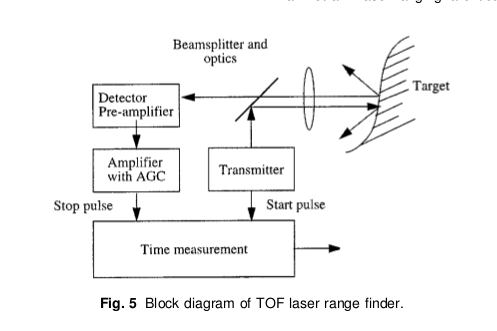
\includegraphics[width=\textwidth]{figures/raycasting/block_diagram.png}
    \caption{\textbf{CHANGE TO TIKZ} Block diagram of \gls{tof} laser range finder\label{fig:lidar_block_diagram}}
\end{figure}
A wide variety of lasers are used depending on the intended measurments range.
In the spacecraft case, laser providing peak energy in the range of \SI{15}{\mega\joule} are often required to measure distance of over \SI{50}{\kilo\meter}~\cite{berry2013}.

The laser range finder is frequently equipped with angle encoders to enable the definition of the position of the measurement point with respect to the sensor. 
Mechanical scanning is performed using a control system which  either move the entire laser range finder or only the measuring beam.
Focal plane scanning is another approach which reduces the mechanical complexity of a mechanical scanning system.
The laser energy illuminates the entire field of view on the surface.
An array of detectors are aranged to view the surface.
Each detector only views a portion of the total field of view and the signals are analyzed in the time domain.
Using this methodology, the system can simulataneously measure distance in multiple directions without any moving parts~\cite{amann2001}.

In the computer graphics field a major problem is the determination of which objects are visible to the user.
In a method similar to the photographic process in reverse, for each pixel of the image a ray is cast towards the scene and the intersections of this ray with any objects is recorded.
The first object which intersects the ray is defined as visible while those beyond would be occluded.
Given this intersection point, the surface normal is computed and surface shading can be determined to render the scene.

Our problem is of a similar nature to that of the computer graphics domain.
Given the model of an asteroid, its shape model, we wish to first simulate measurements of the surface. 
In order to simulate these methods, we must also implement a ray casting algorithm that will find the intersection of a measurement from the spacecraft to the surface. 

We assume that the spacecraft is located at \(\rpos\) in the asteroid fixed frame.
The camera/sensor is aligned with \gls{view_axis} in the spacecraft fixed frame.
An additional vector, defined as the up axis \gls{up_axis}, finally the standard basis is completed with \(  \gls{right_axis} = \gls{view_axis} \times \gls{up_axis} \) which defines a reference frame attached to the image plane of the sensor.
Furthermore, we model the the laser ranging sensor as having a fixed field of view defined by the angles \( \gls{fov_h}, \gls{fov_v}\), defining the vertical and horizontal fields of view.
In order to simulate depth measurements we need to determine the transformation of locations in the image frame to the asteroid frame. 
Given the view axis, and a chosen distance \gls{view_distance}, we can define a viewing \gls{frustum} associated with the sensor. 
We can compute the vectors associated with the maximum extents of the far plane as follows.
The half height and width of the far plane, at a distance \( d \), is computed as
\begin{align*}
    H = d \tan \frac{\alpha}{2} , \\
    W = d \tan \frac{\beta}{2} .
\end{align*}
From these values, the extents of the far plane are defined by the vectors
\begin{align*}
    A = \vc{c}_1 + H \vc{c}_3 - W \vc{c}_2 , \\
    B = \vc{c}_1 + H \vc{c}_3 + W \vc{c}_2, \\
    C = \vc{c}_1 - H \vc{c}_3 + W \vc{c}_2, \\
    D = \vc{c}_1 - H \vc{c}_3 - W \vc{c}_2.
\end{align*}
The view frustrum is visualized in~\cref{fig:view_frustrum} and allows for any vector in the field of view to befined as a linear combination of the extents of the far plane.
\begin{figure}[htbp]
    \centering
    \includegraphics[width=\textwidth]{example-image-golden}
    \caption{View Frustrum for Spacecraft sensor modeling\label{fig:view_frustrum}}
\end{figure}

\section{Incremental Radius modification}\label{sec:radius_update}

One of the first main tasks for any spacecraft mission to an asteroid is to generate an estimate of the asteroid shape.
This shape model is used for a variety of purposes, such as the polyhedron potential model, like that presented in~\cref{sec:polyhedron_potential} or landing site section and guidance.
We assume that upon arrival at a target body, the spacecraft contains an initial estimate for the shape of the asteroid.
This shape can be a coarse estimate computed from ground measurements or it can be a triaxial ellipsoid based on the semimajor axes of the asteroid, such as that shown in~\cref{fig:start} which represents the maximum axes for asteroid Castalia.
Additionally, we assume that the shape estimate is closed and a triangular faceted surface mesh, emulating those used in practice to represent asteroids.
Furthermore, the number of vertices in the estimate can be scaled according to the desired final acccuracy or computational capabilities.
For example,~\cref{fig:uniform_mesh} demonstrates two surface mesh representation for a triaxial ellipsoid at varying levels of detail. 
A wide variety of algorithms are available to generate a near uniformly spaced mesh for an arbitrary surface~\cite{persson2004,boissonnat2005}.
\begin{figure}[htbp]
    \centering
    \subcaptionbox{Coarse Uniform Mesh\label{fig:coarse_uniform_mesh}}{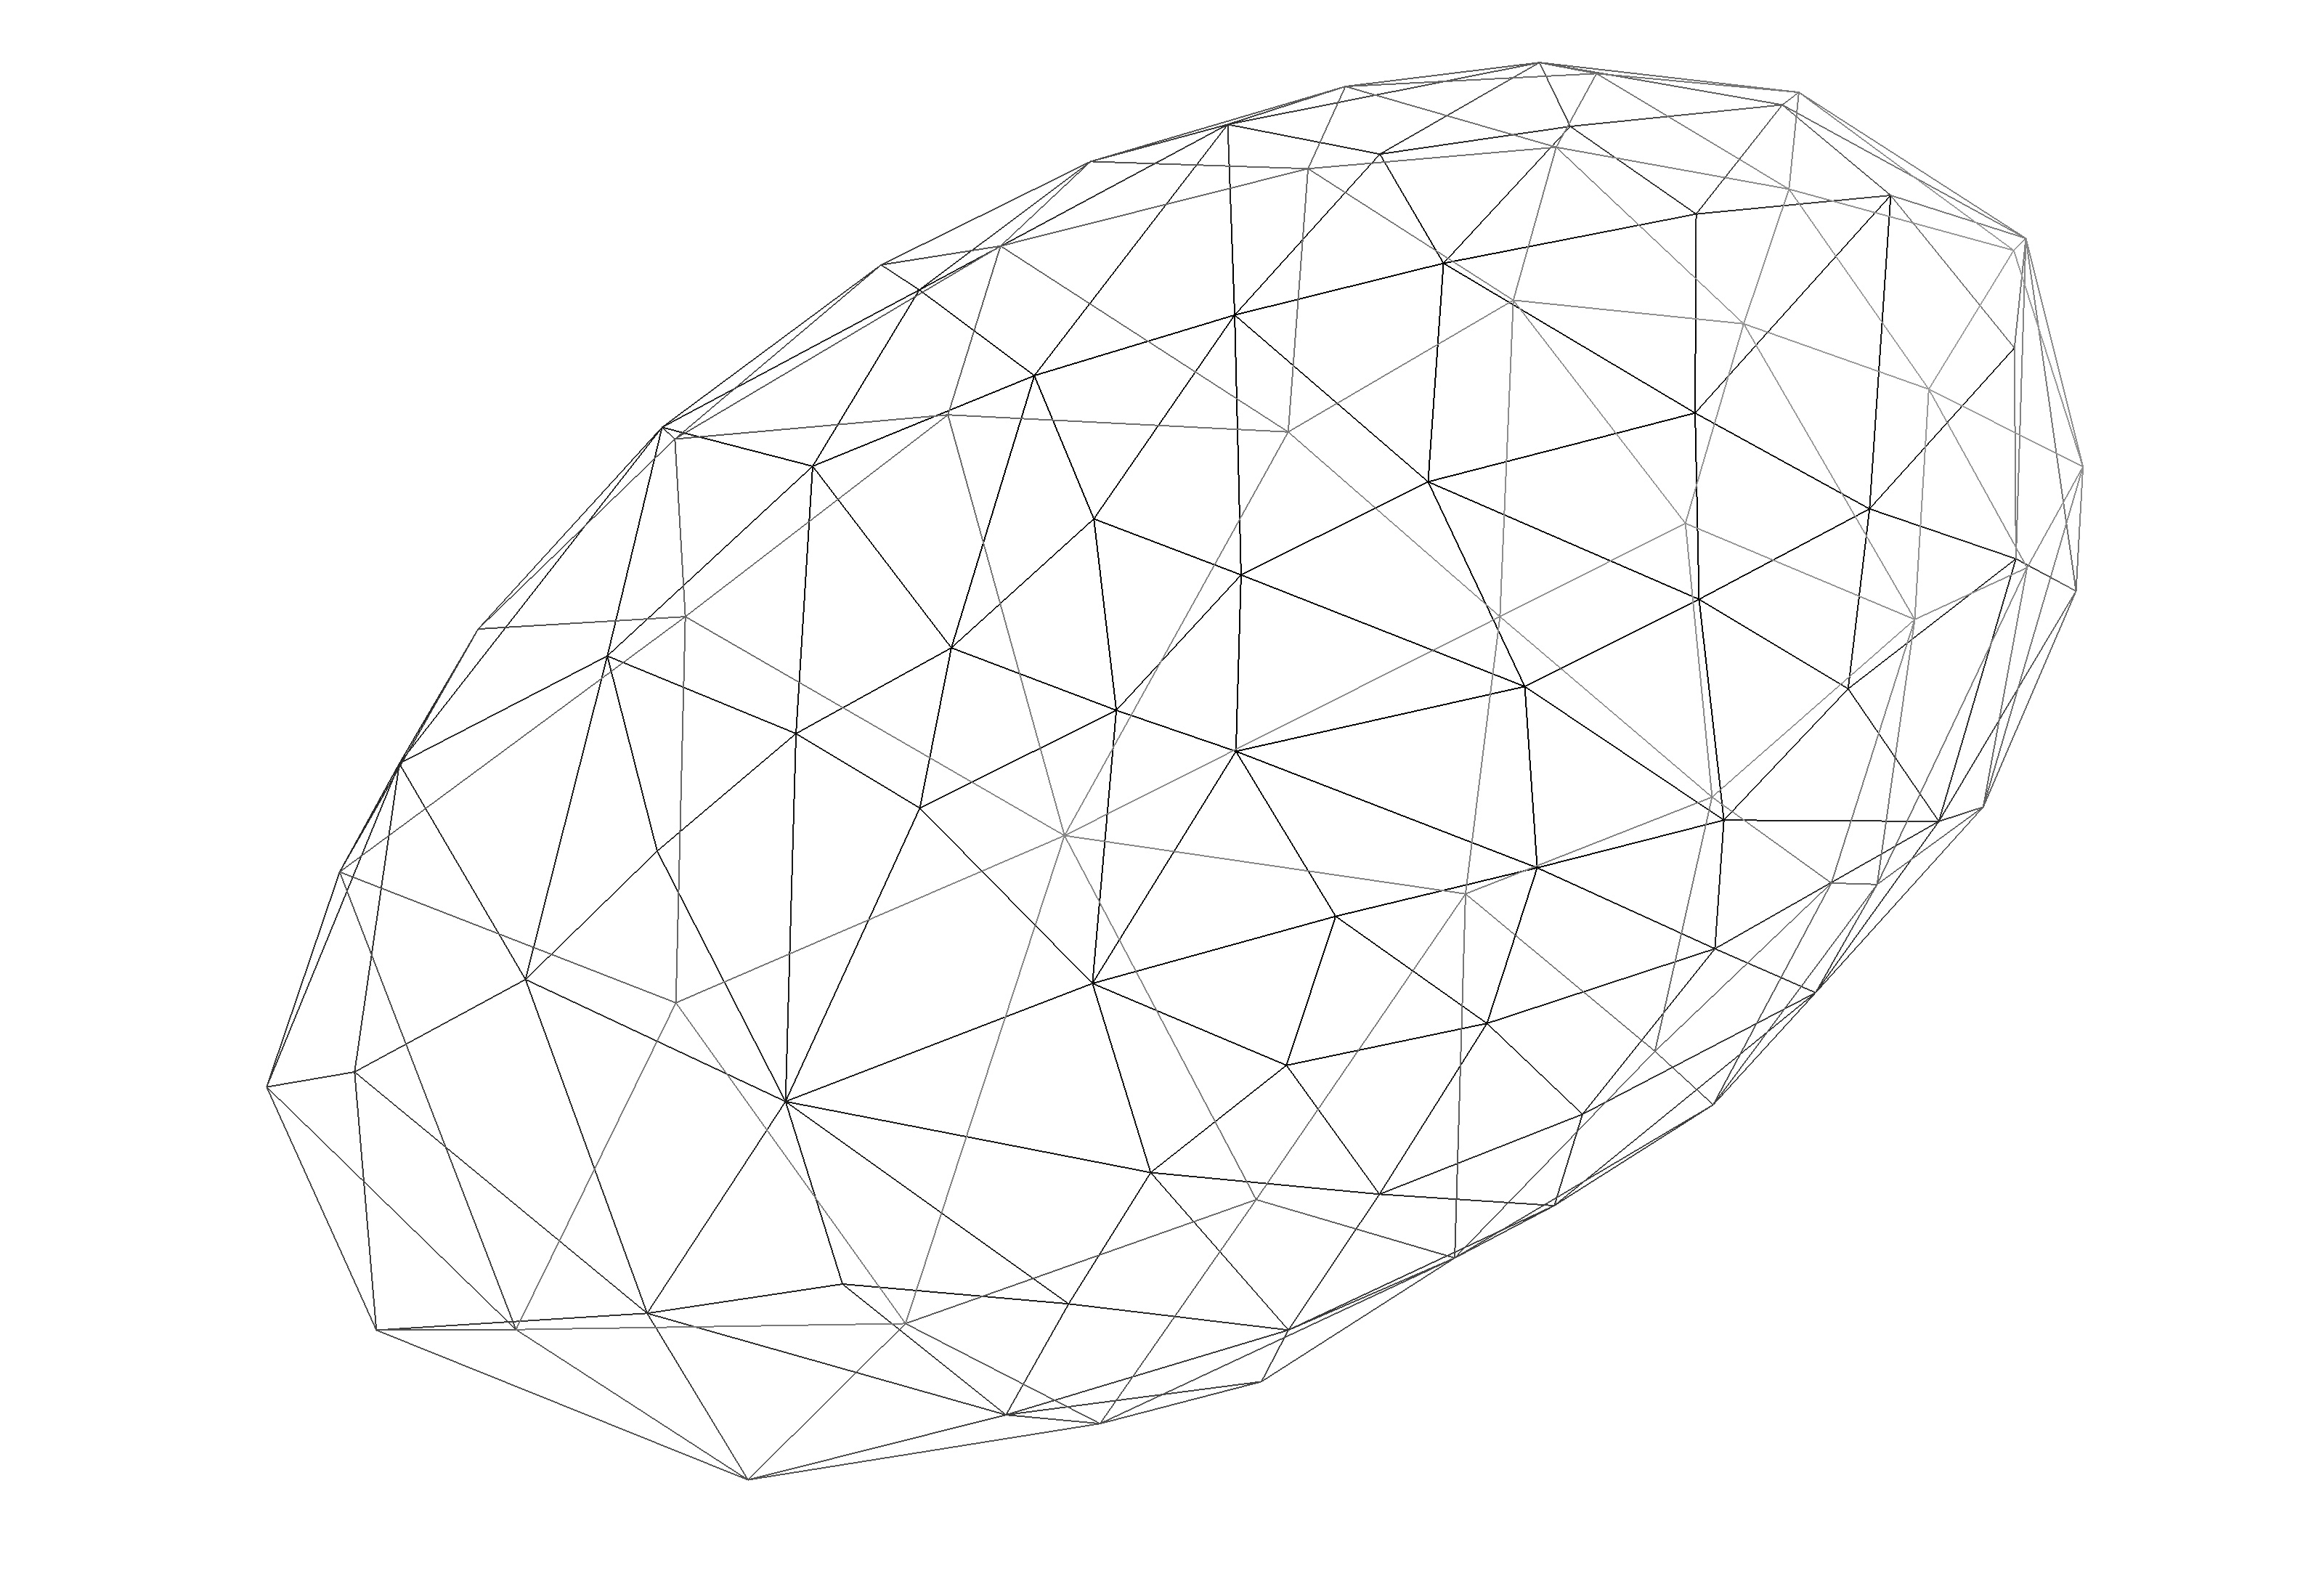
\includegraphics[width=0.5\textwidth]{figures/computational_geometry/uniform_mesh_coarse.jpg}}~
    \subcaptionbox{Fine Uniform Meesh\label{fig:fine_uniform_mesh}}{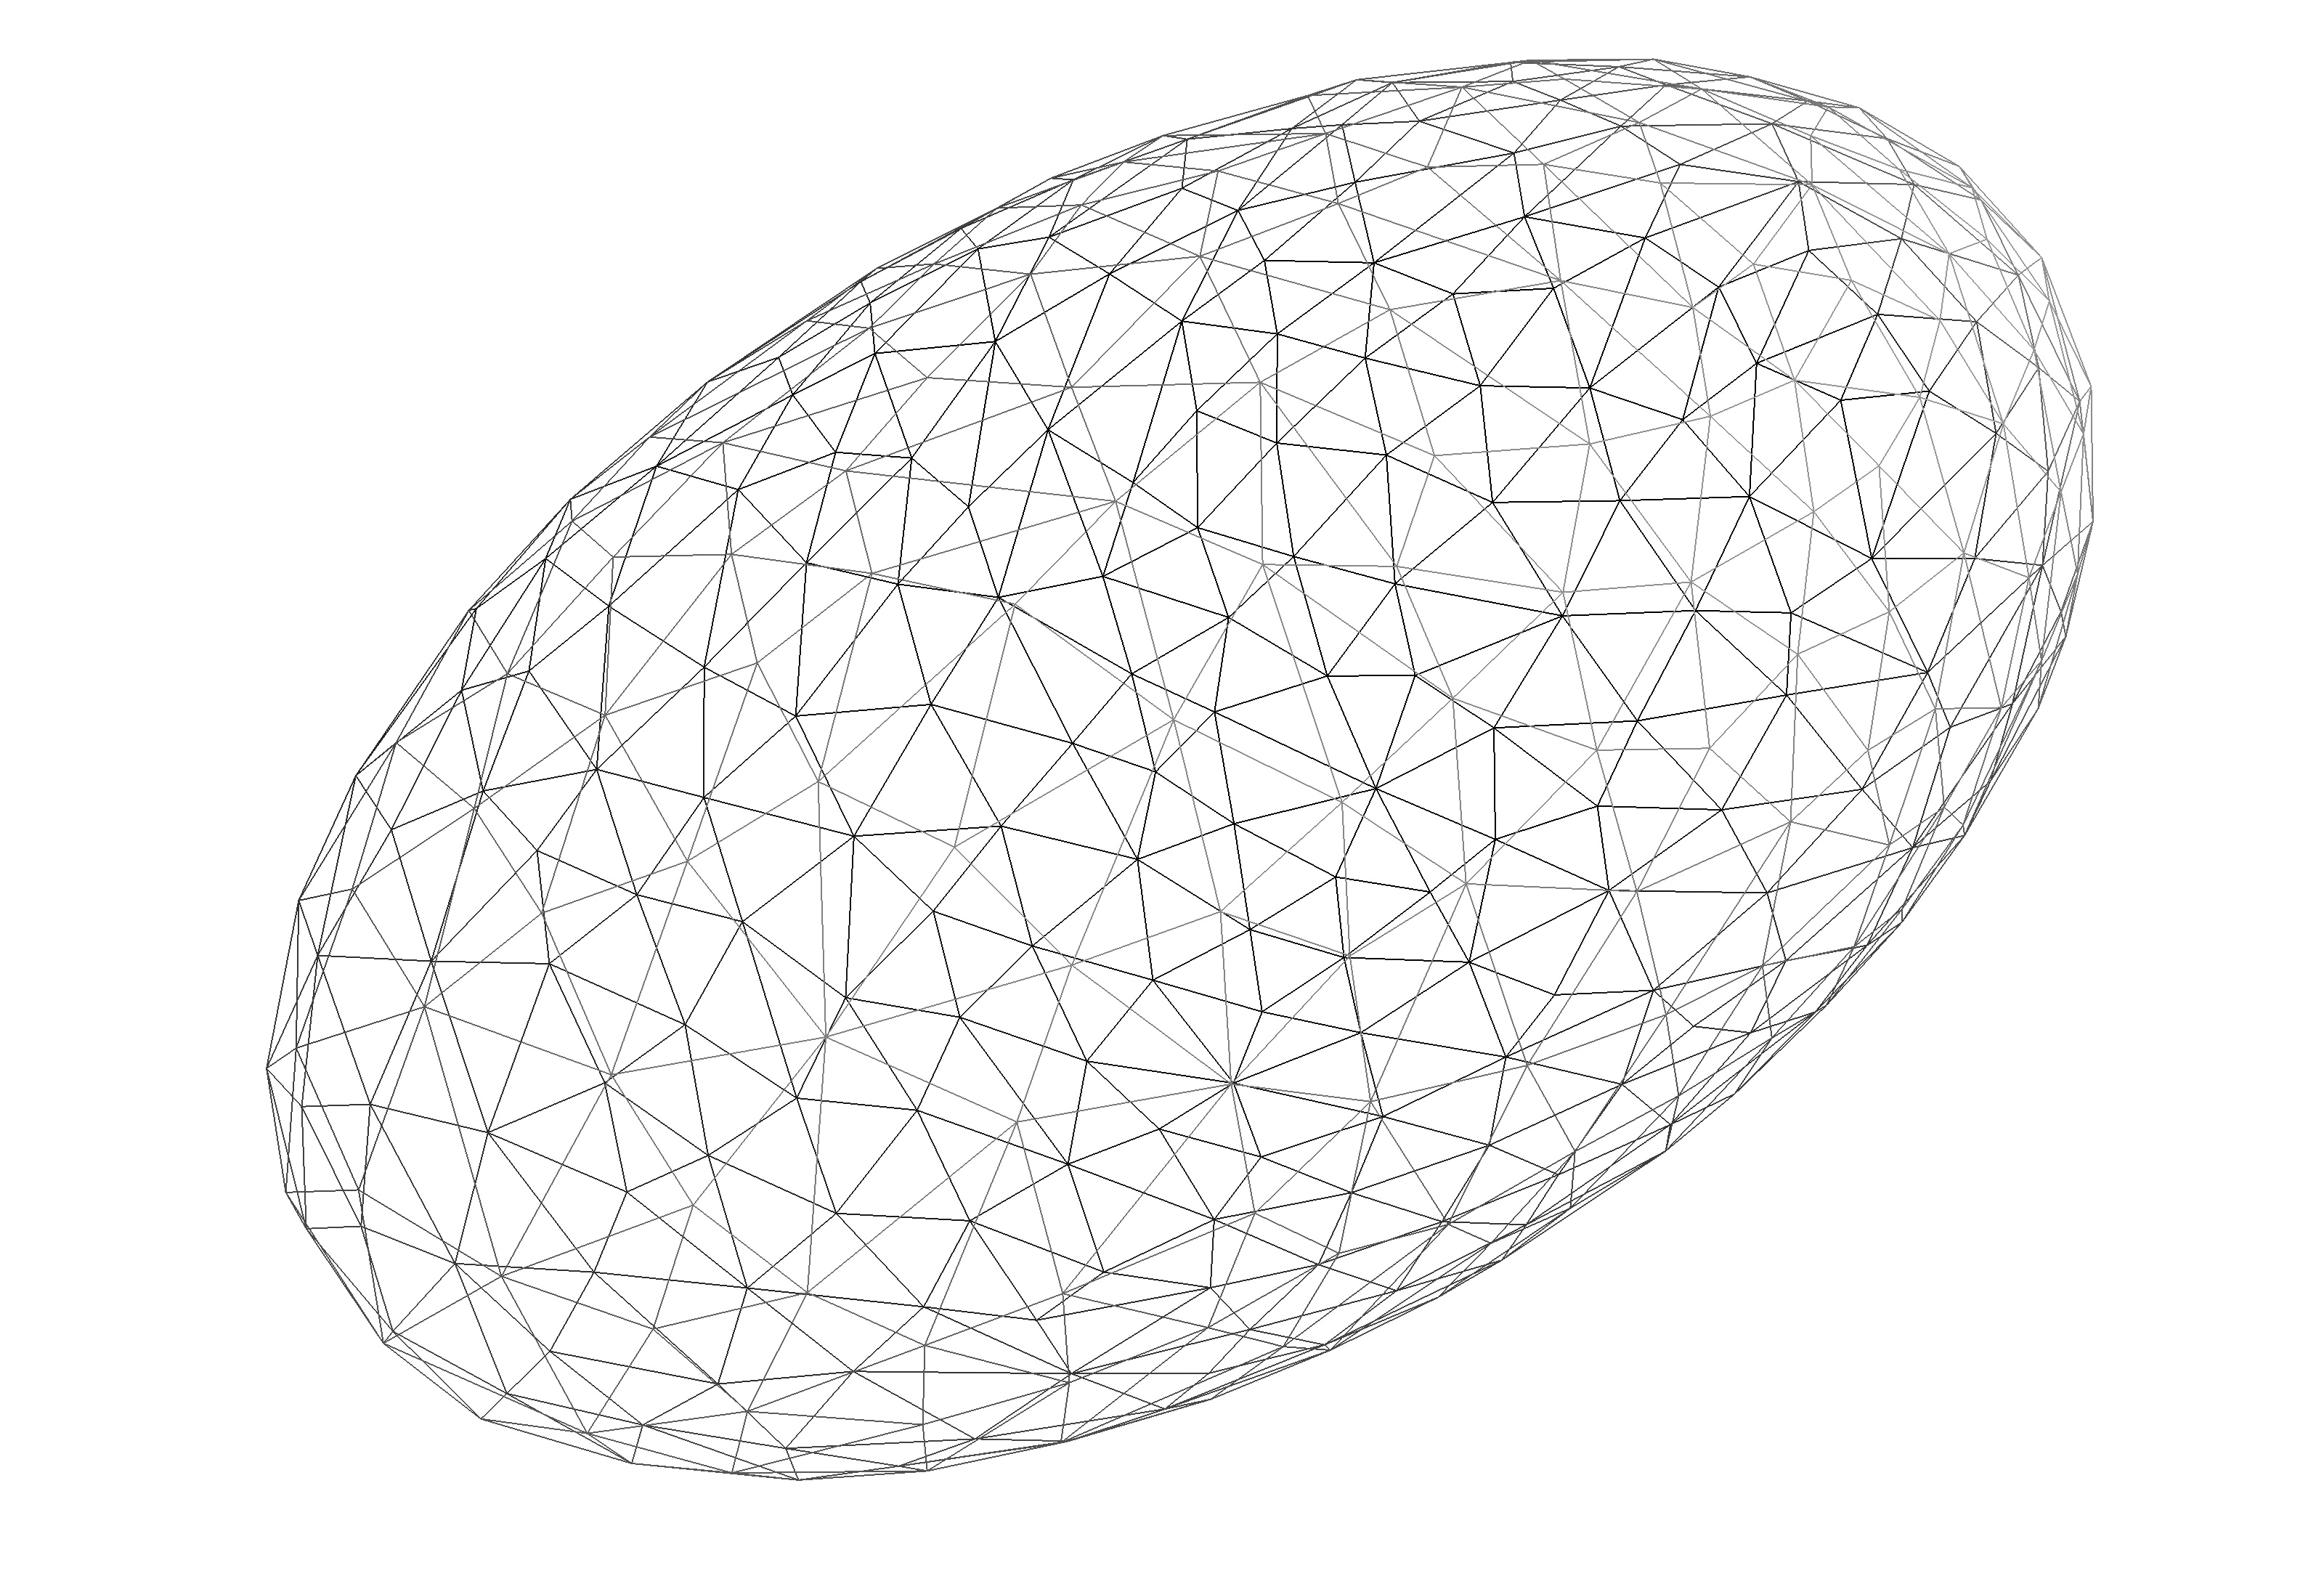
\includegraphics[width=0.5\textwidth]{figures/computational_geometry/uniform_mesh_fine.jpg}}
    \caption{Examples of Resolution of Uniform Meshes of Triaxial Ellipsoid~\label{fig:uniform_mesh}}
\end{figure}

\begin{figure}
    \centering
    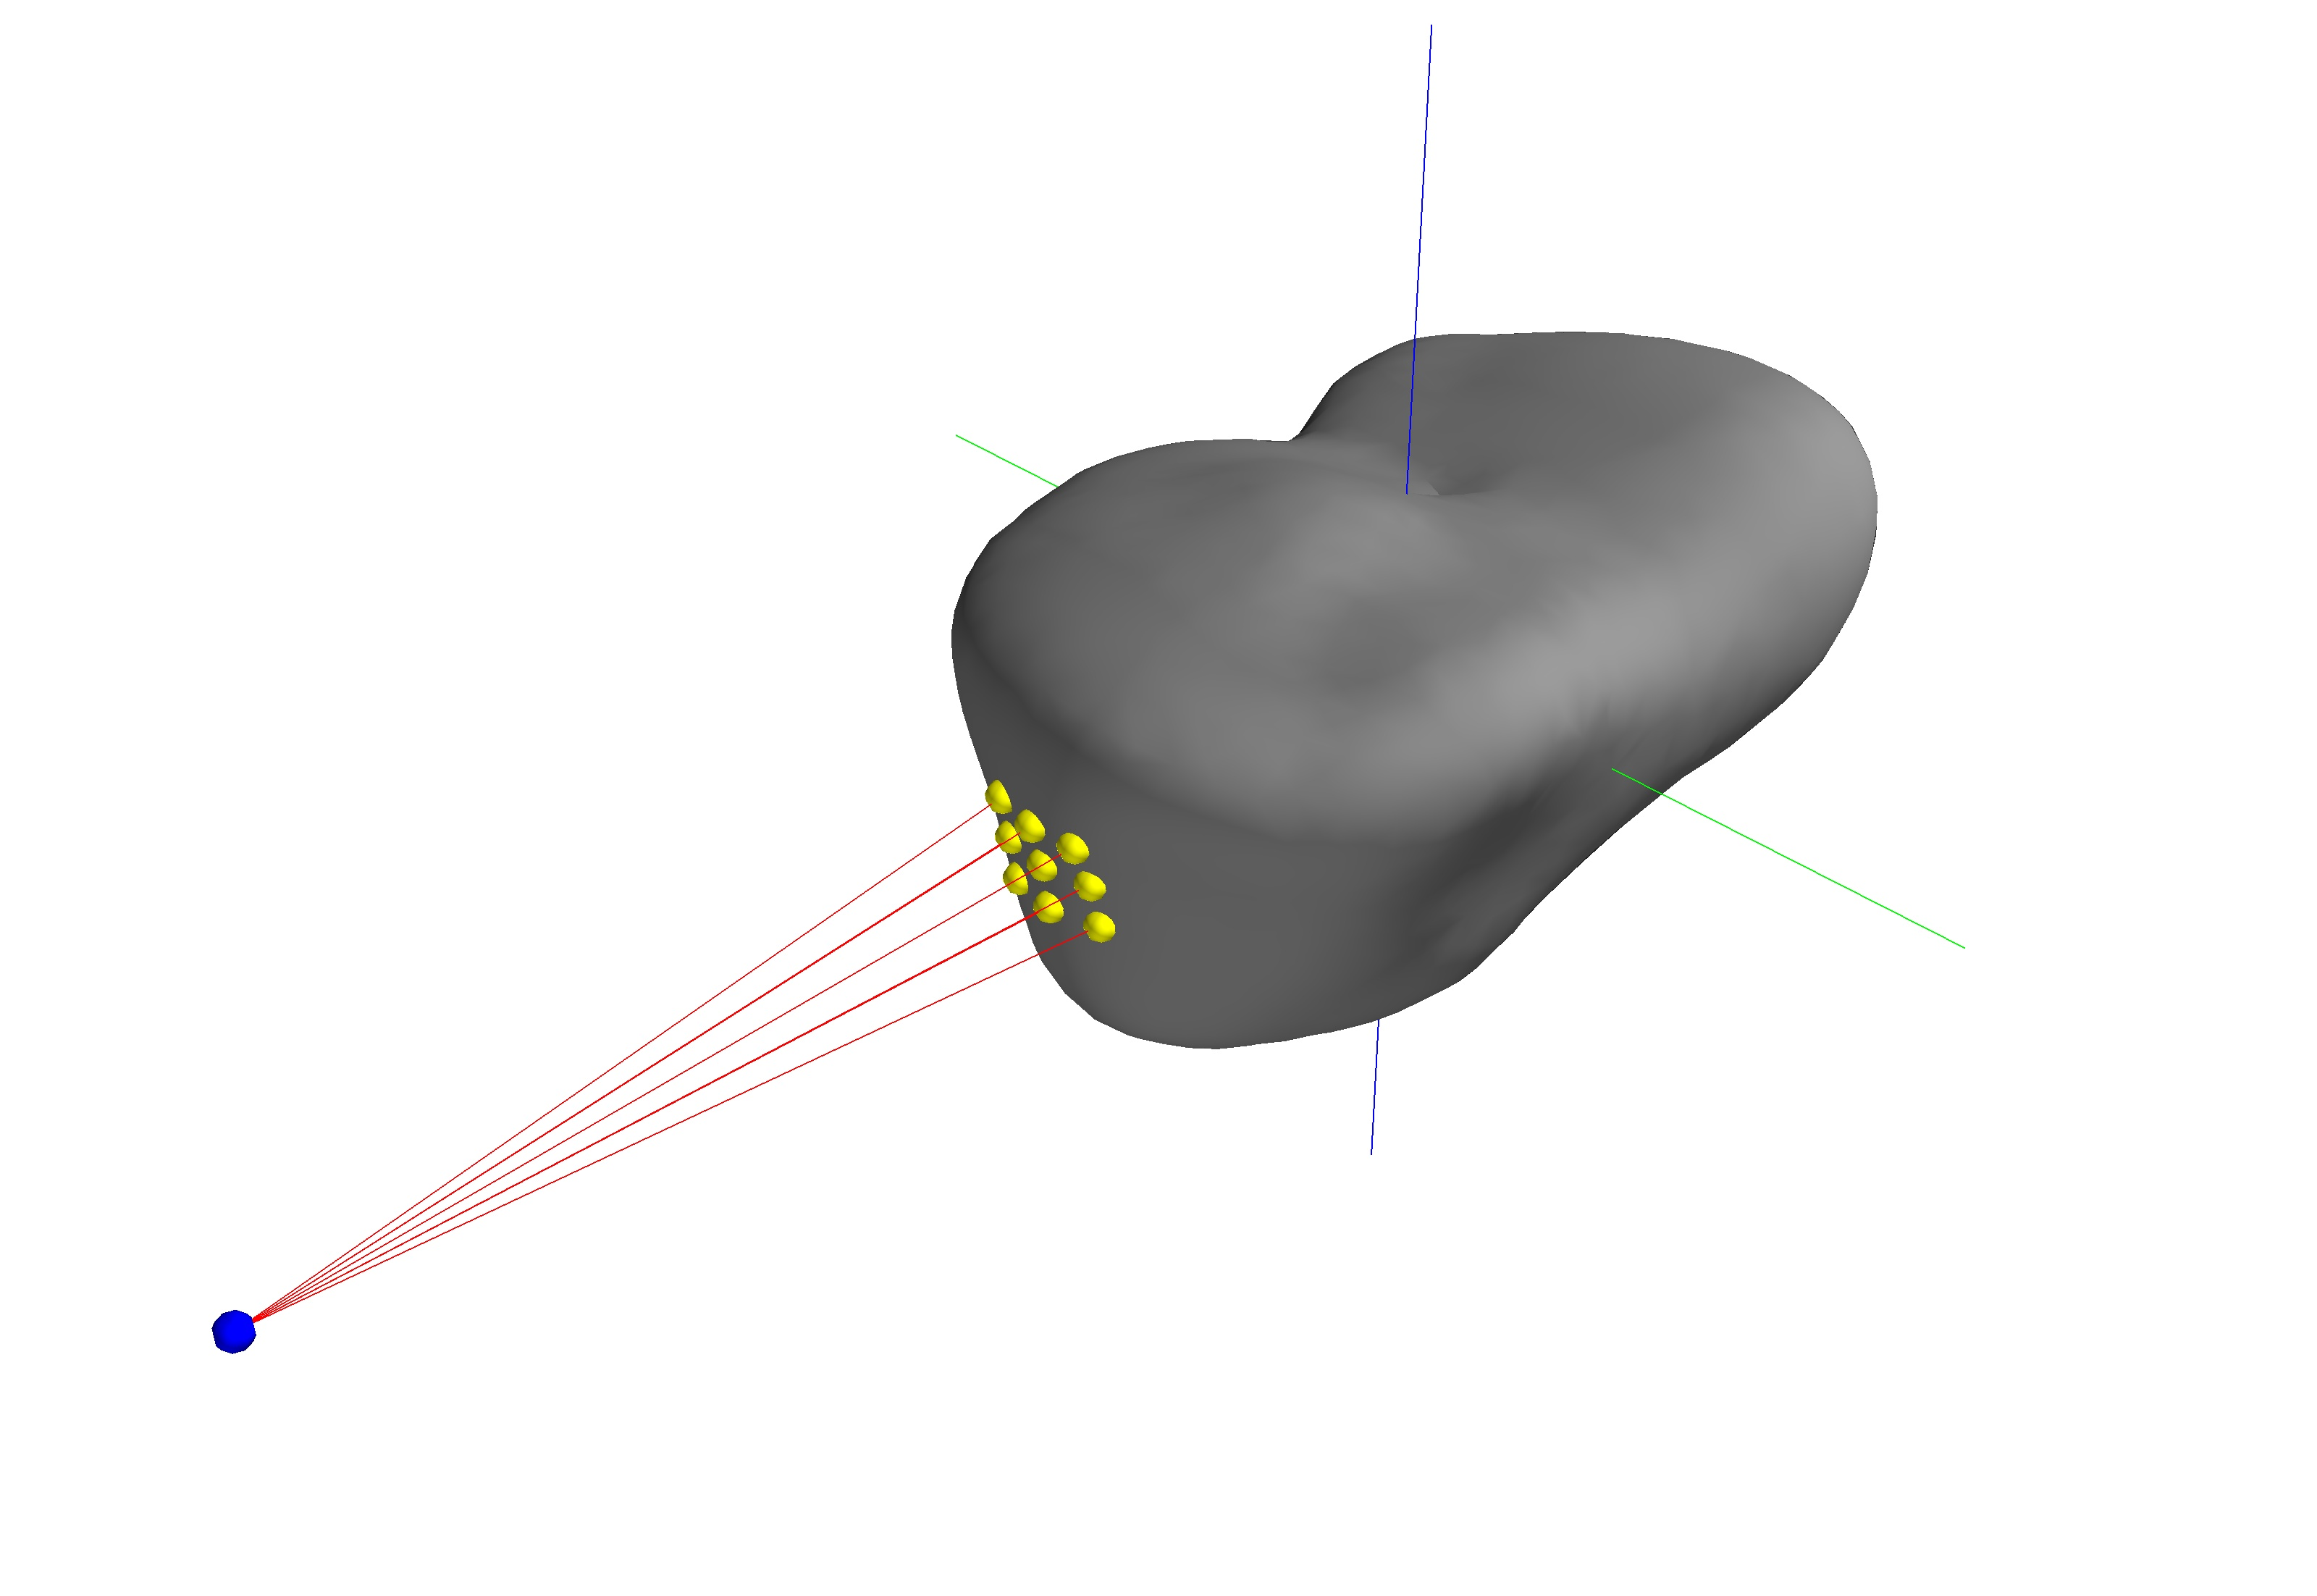
\includegraphics[width=0.75\textwidth]{figures/2018_SSPI/castalia_raycasting_plot.jpg}
    \caption{Simulated LIDAR measurements of asteroid Castalia~\label{fig:lidar_example}}
\end{figure}
We assume the spacecraft contains a range sensor, such as LIDAR, that allows for the accurate measurement of the relative distance between the spacecraft and asteroid~\cite{zuber1997,zuber2000}.
This type of sensor measures the round-trip time for a pulse of energy to leave the spacecraft, reflect off the surface, and return to a collector on board.
Given the time total time of flight, the distance can be accurately computed using \( d = \frac{\Delta TOF}{2 c} \) where \gls{sym:c} is the constant speed of light.
Assuming accurate knowledge of the pointing direction of the spacecraft we can compute a direction from the spacecraft to the measurement location on the surface.
The output of this sensor is a vector, \( \vc{d}_i \), defined in the spacecraft fixed frame which gives the direction to a measurement point on the surface of the asteroid. 
Using the state of the asteroid, we can transform this measurement to the asteroid fixed frame using the simple transformation
\begin{align*}
    \vc{p}_i = R_A^T R \vc{d}_i .
\end{align*}
Given many measurements, \( \vc{p}_i \), of the asteroid surface we can efficiently update our initial shape estimate to that of the true surface.
\Cref{fig:lidar_example} shows asteroid 4769 Castalia and a representation of several LIDAR measurements. 
The spacecraft measures the range between itself and the asteroid surface to several points within the field of view of the sensor. 
These measurements provide a collection of points which lie on the surface of the asteroid, and by combining many points, a so called ``point cloud'', allows us to reconstruct the shape.
% TODO Discuss point cloud reconstruction approaches (all computational exspensive and designed for unknown surfaces)

Our algorithm applies a Bayesian framework to radially modify each vertex \( \vc{v}_i \in \R^3\) of the shape estimate based on measurement \( \vc{p}_i \in \R^3 \). 
This approach alleviates much of complexity of incorporating new vertices or surface triangulation common in surface reconstruction methods~\cite{berg2008}.
This assumption means that the total number of vertices of the shape model is fixed.
However, additional detail, in the form of additional vertices, is possible by using standard mesh subdivision algorithms~\cite{orourke1998}, which we demonstrate in a subsequent section.

The radial distance of each vertex, \( v_i = \norm{\vc{v}_i}\), is assumed to be distributed according to the Gaussian distribution
\begin{align*}
    v_i \sim \mathcal{N}(r_i, w_i^2)
\end{align*}
where \( r_i \) is the initial estimate of the radial distance of vertex \( \vc{v}_i\) and \( w_i \) is the initial variance, or confidence, in the radial distance.
The radial distance of each measurement, \( p_{j,i} = \norm{\vc{p}_j}\), is also assumed to be distributed according to the Gaussian distribution
\begin{align*}
    p_{j,i} \sim \mathcal{N}(r_{j,i}, w_{j,i}^2)
\end{align*}
where \( r_{j,i} = \norm{\vc{p}_{j,i}} \) defines the radial distance of the surface vector measurement and \( w_{j, i}\) defines the variance of the measurement with respect to vertex \( \vc{v}_i\).
Each measurement is defined by the index \( j \) while the associated vertex is defined by \( i \). 
As a result, the measurement \( p_{j, i} \) defines the distribution of measurement \( j \) with respect to vertex \( i \). 
Any given measurement may be used to update one or several vertices.

The variance for each measurement vector is assumed to be related to the ``distance'' from the measurement to vertex \( \vc{v}_i \).
Here we use the \gls{geodesic} distance to parameterize the difference, and hence  uncertainty, of associating the measurement with a given vertex.
From spherical trigonometry~\cite{gade2010} the central angle between measurement \( \vc{p}_i \) and vertex \( \vc{v}_i \) of the shape estimate is
\begin{align}\label{eq:geodesic_distance}
    \Delta \sigma_{j,i} = \arctan \parenth{\frac{\norm{\vc{p}_j \times \vc{v}_i}}{\vc{p}_j \cdot \vc{v}_i }}.
\end{align}
The variance of measurement \( \vc{p}_i \) with respect to vertex \( \vc{v}_i \) is then defined as the arc length as
\begin{align}
    w_{j, i} = \norm{\vc{p}_j} \Delta \sigma_{j,i} .
\end{align}
This approach relates the uncertainty of the measurement, \( \vc{p}_j \) with the geodesic distance to a given vertex, \( \vc{v}_i \).
As a result, measurements which are far from a vertex, where \( \Delta \sigma \) is large, will tend to have a larger variance and hence uncertainty. 
This approach can be considered as a form of a correlation based sensor model~\cite{thrun2005}.
The main benefit of a correlation based approach, in constrast to feature extraction is the relative simplicity of implementation.
However, the resulting correlation values do not posses any physical significance and do not represent the noise or uncertainty characteristics of the sensor.

From Bayes' theorem, the posterior probability is
\begin{align}
    p(v_i | p_{j, i}) = \frac{p(p_{j, i} | v_i) p(v_i)}{p( p_{j, i})} \propto p(p_{j,i} | v_i) p(v_i).
\end{align}
From the properties of a Gaussian, the posterior probability given a measurement is also distributed according to a Gaussian distribution~\cite{bishop2006} and given by
\begin{align}\label{eq:posterior_probability}
    \mathcal{N} \parenth{\frac{w_{j, i}^2 r_i + w_i^2 r_{j, i}}{w_i^2 + w_{j, i}^2} , \frac{w_i^2  w_{j, i}^2}{w_i^2 +  w_{j, i}^2}} .
\end{align}
From~\cref{eq:posterior_probability}, the posterior probability conditioned on the measurement is the weighted average of the prior knowledge and the measurement. 
Measurements that are far from the vertex will have a high uncertainty or variance and will have a reduced impact on the radial position of the vertex.
Additional measurements are incorporated using a weighted average of prior belief and the measurement uncertainty.

In order to improve the computational efficiency measurement updates are assumed to be local in nature.
Instead of applying a measurement to all vertices of the mesh, the measurement is only applied to the vertices which are within a specified region of the measurement. 
We define a region of interest, \( \Delta S \), about each measurement which defines the surface area over which the measurement will affect the mesh estimate.
We relate \( \Delta S \) to an equivalent angular constraint using
\begin{align}\label{eq:region_of_interest}
    \Delta \sigma_{max} = \sqrt \frac{\Delta S}{r_b^2}
\end{align}
where \( r_b \) defines the Brillouin  sphere radius, or the radius of the circumscribing sphere of the asteroid.
Only vertices which satisfy \( \Delta \sigma_i \leq \Delta \sigma_{max} \) are considered in the Bayesian update shown in~\cref{eq:posterior_probability}.

The approach presented in~\cref{sec:radius_update} allows one to update the shape of an asteroid given a single range measurement of the surface.
A sequential process can be used to iteratively update the shape estimate given many measurements of the surface. 
For example,~\cref{fig:reconstruction} illustrates the process of updating an initial shape estimate of asteroid 4769 Castalia.
The initial shape for Castalia is a triaxial ellipsoid with semi-axes equal to \( \SI{1.8}{\kilo\meter} \times \SI{0.8}{\kilo\meter} \times \SI{0.8}{\kilo\meter}\) and shown in~\cref{fig:start}.

Simulated measurements of the surface of 4769 Castalia are used to update the initial mesh estimate.
The truth shape model, and the associated vertices, are used as simulated measurements of the shape of Castalia~\cite{neese2004}.
The true shape model of 4769 Castalia is composed of \num{2048} vertices and \num{4092} triangular faces.
The initial shape estimate is chosen to have approximately the same number of vertices as the final true shape and such that the total number of vertices remains constant.
\begin{figure}[htbp]
    \centering
    \subcaptionbox{Initial mesh estimate\label{fig:start}}{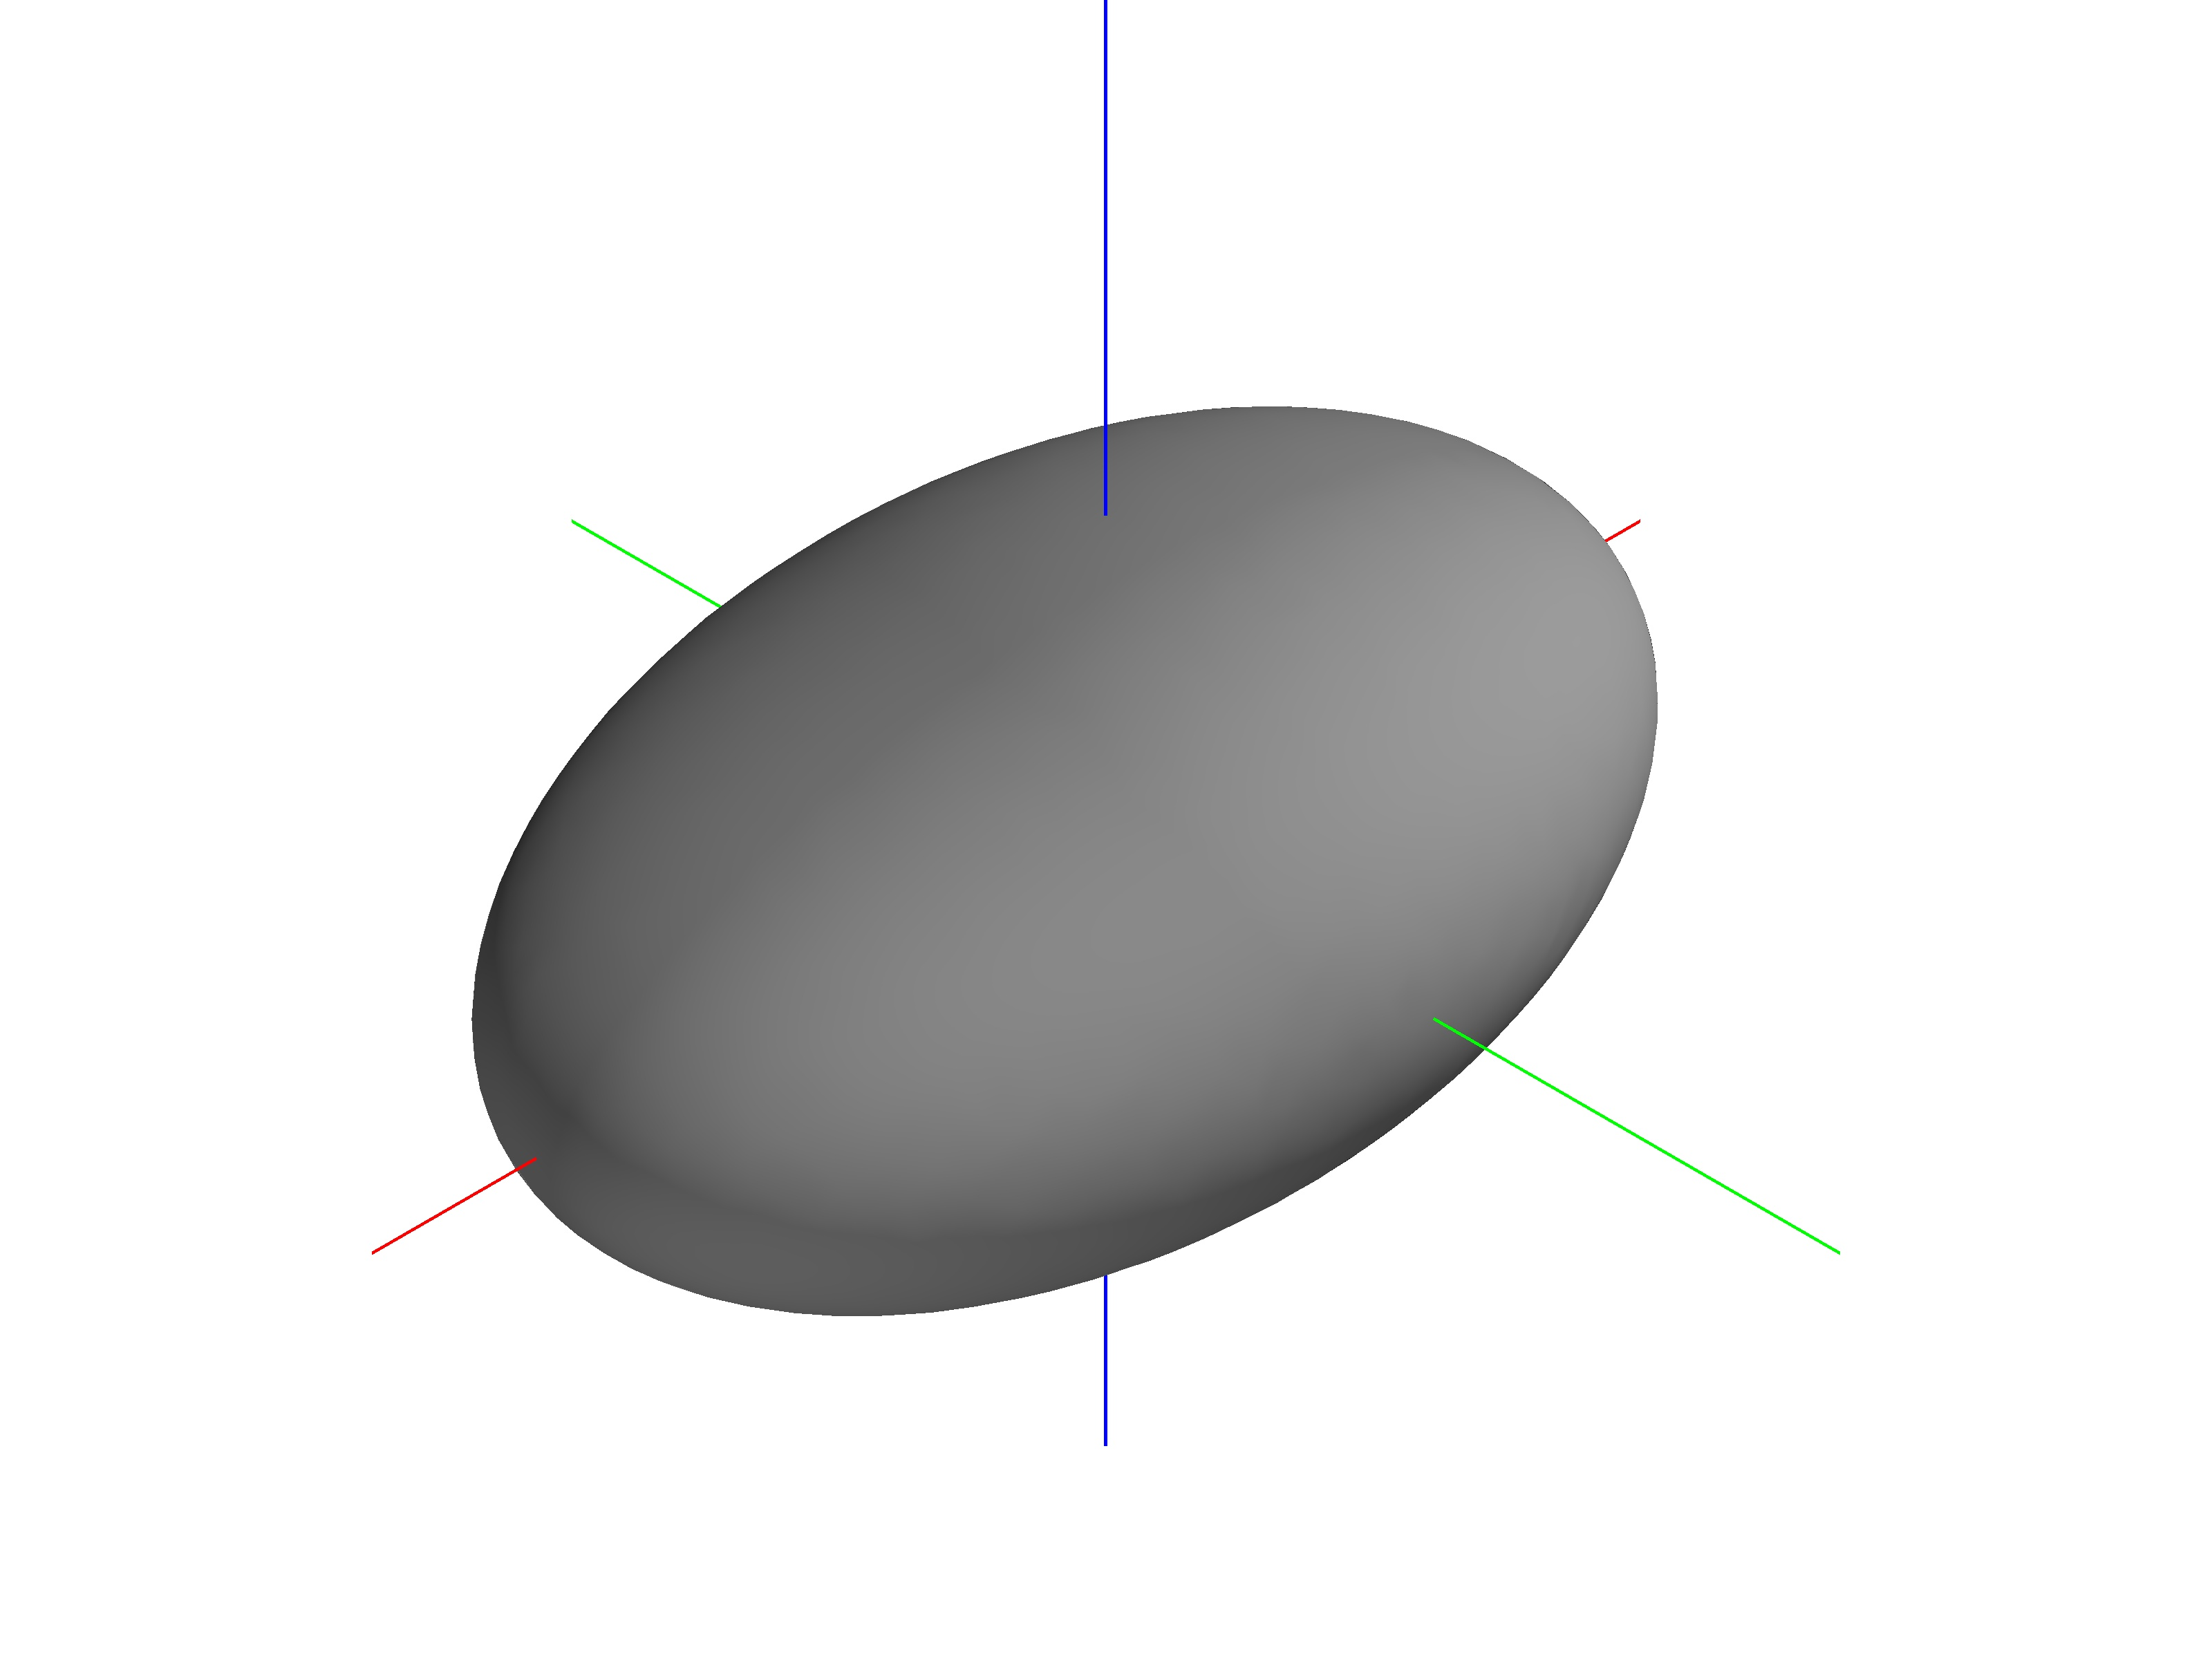
\includegraphics[height=0.5\textheight,width=0.5\textwidth,keepaspectratio]{figures/2018_SSPI/partial_initial.jpg}}~
    \subcaptionbox{First measurement added\label{fig:first}}{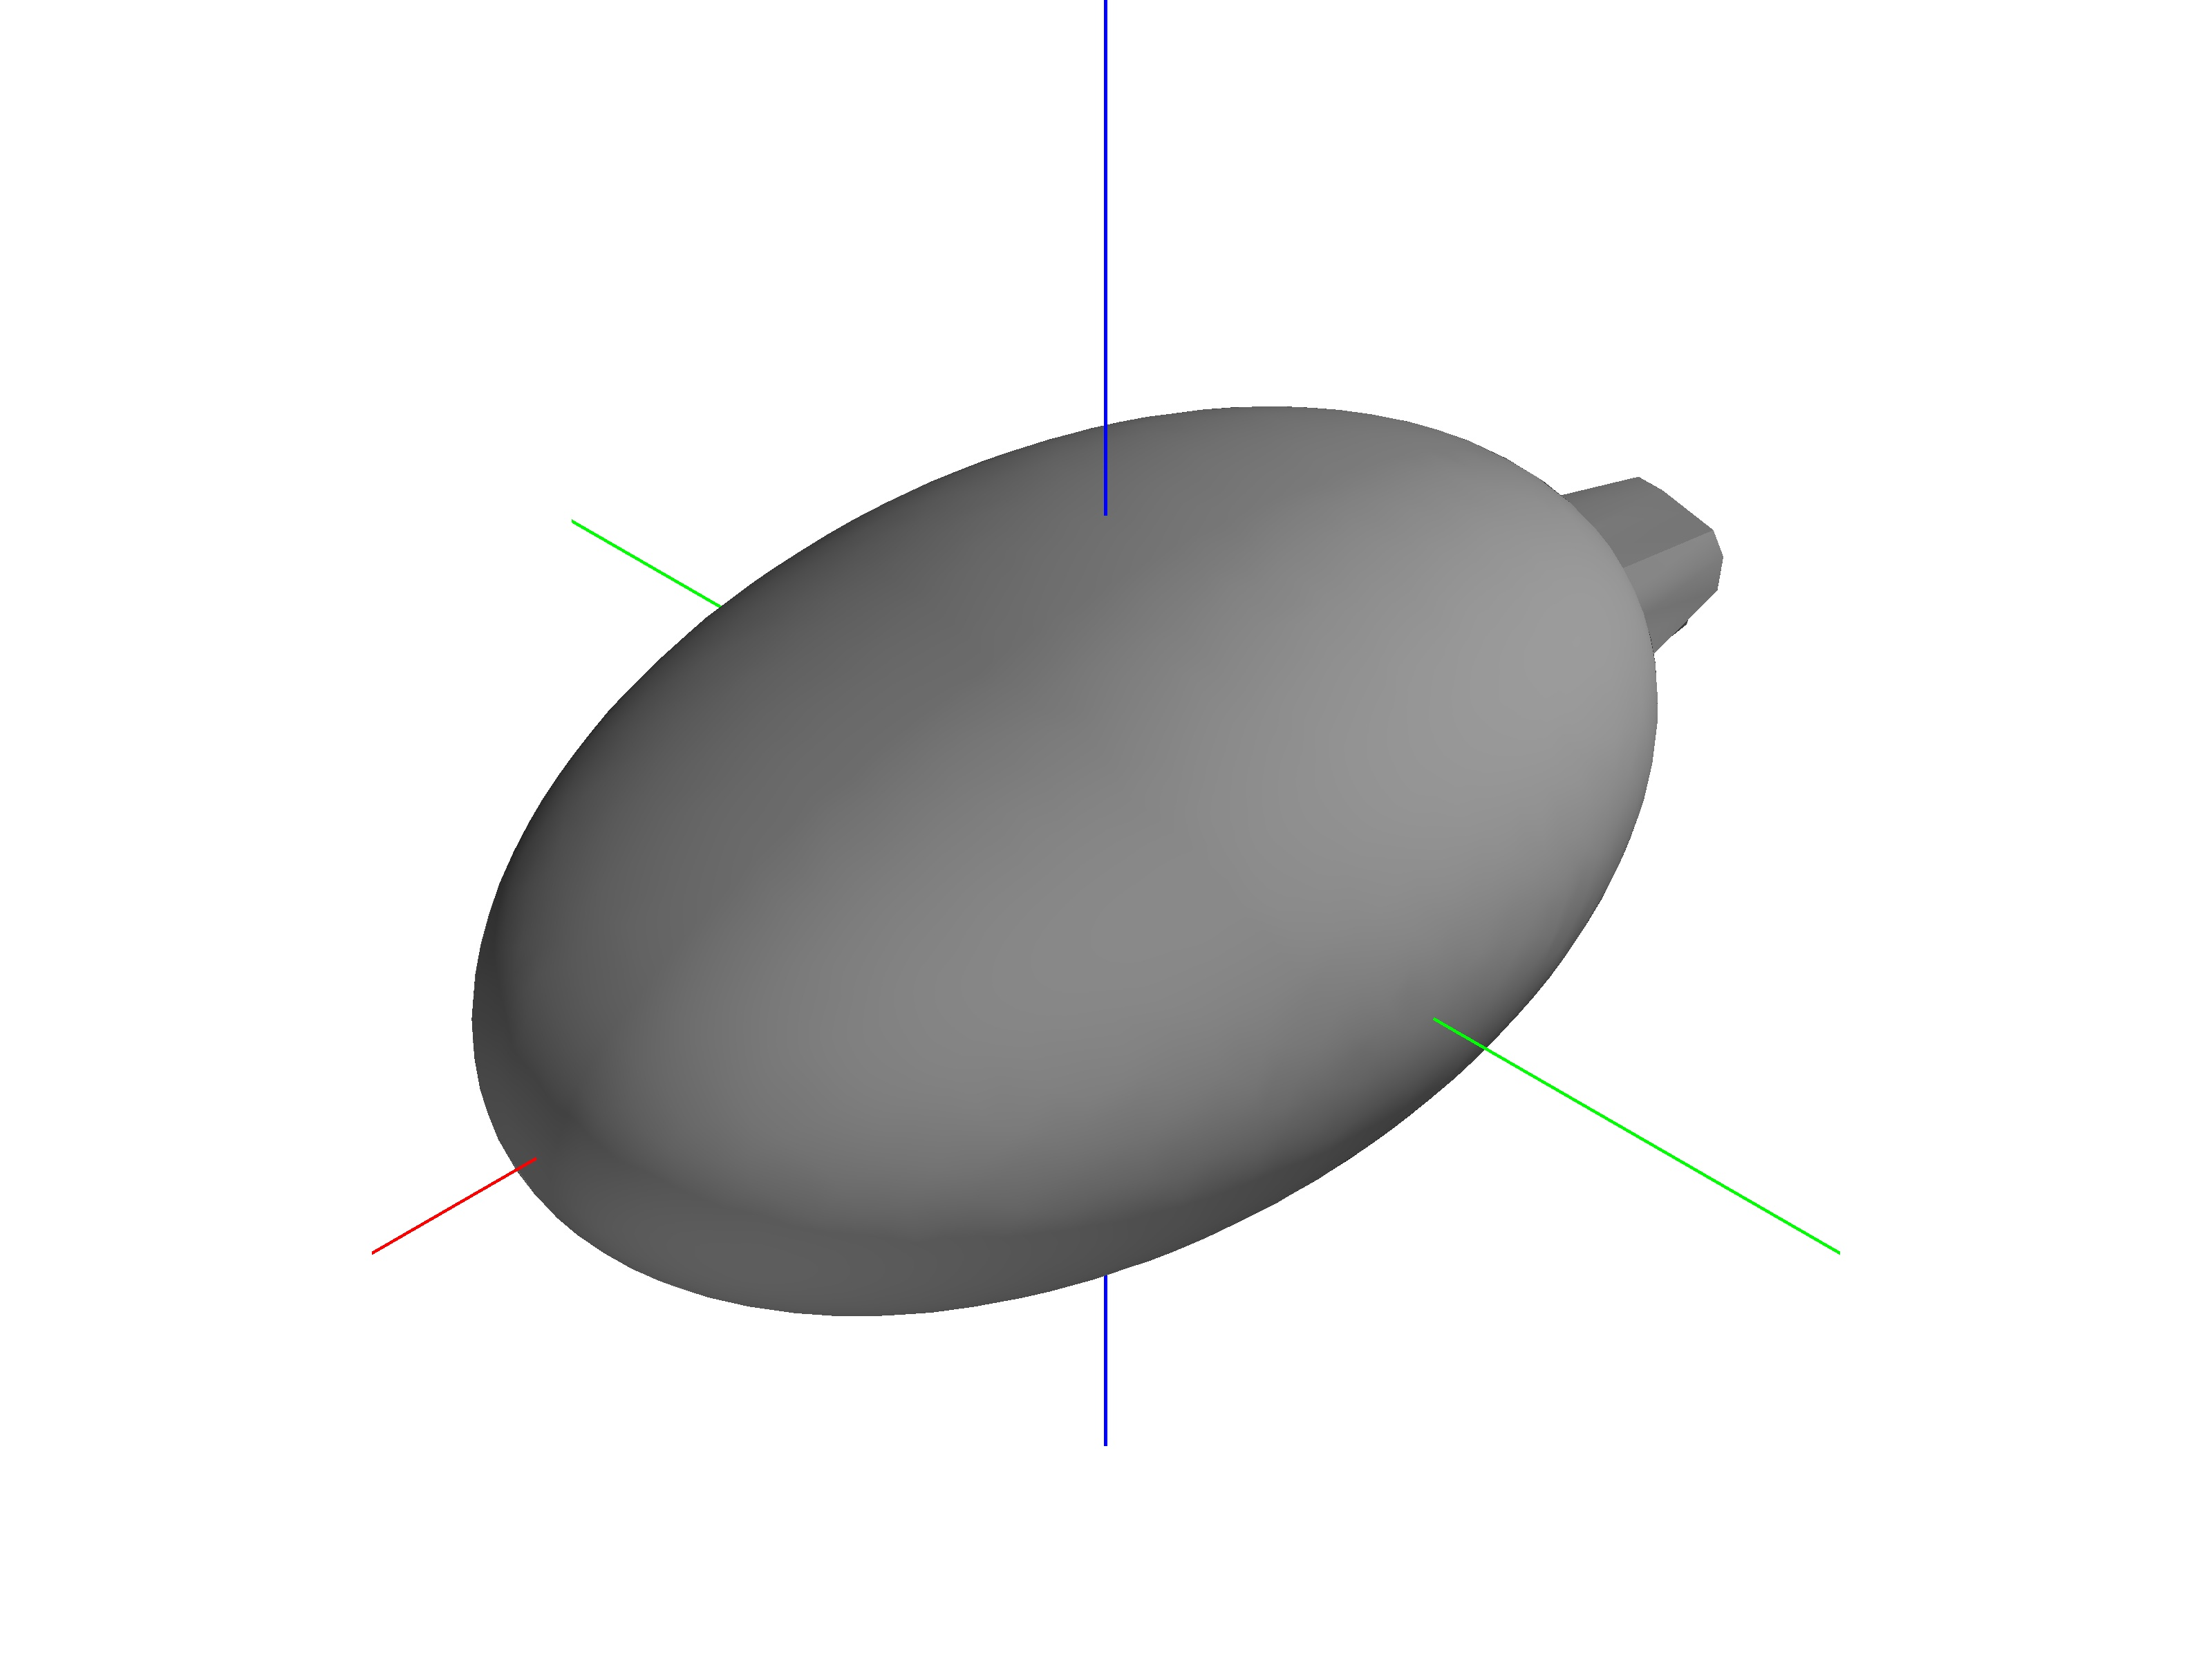
\includegraphics[width=0.5\textwidth]{figures/2018_SSPI/partial_0.jpg}}

    \subcaptionbox{\SI{25}{\percent} of measurments added\label{fig:quarter}}{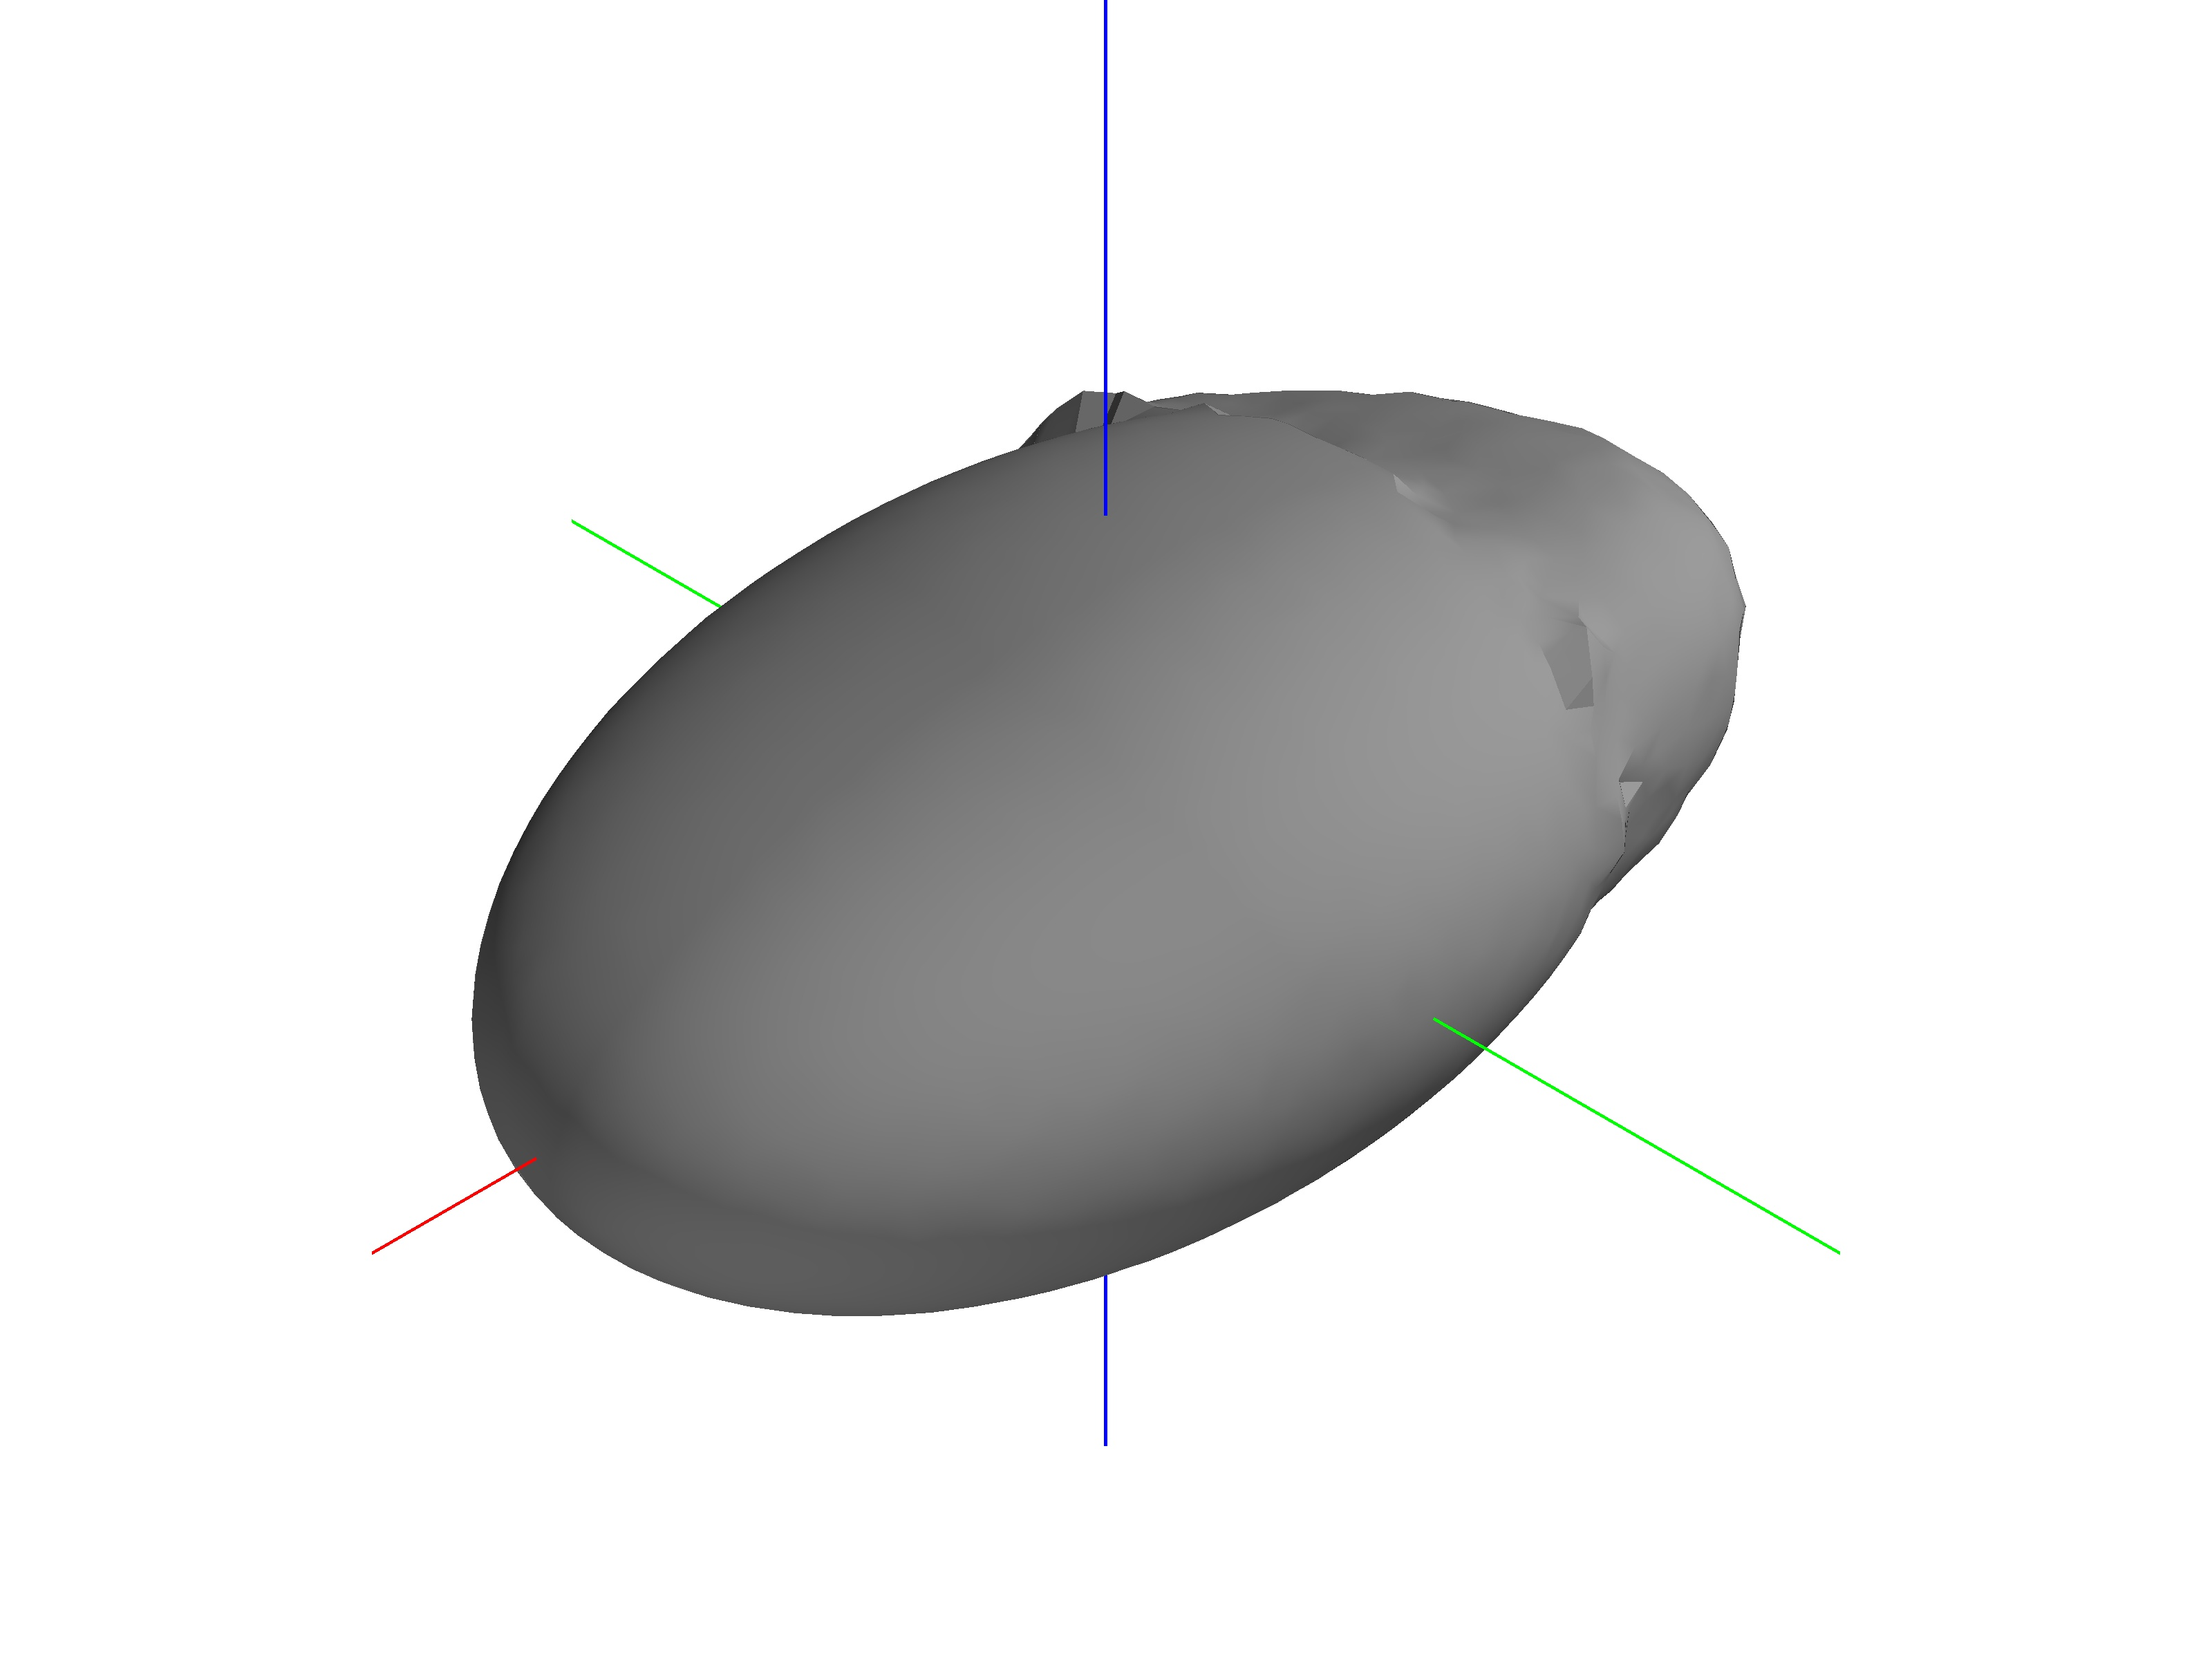
\includegraphics[width=0.5\textwidth]{figures/2018_SSPI/partial_512.jpg}}~
    \subcaptionbox{\SI{50}{\percent} of measurements added\label{fig:half}}{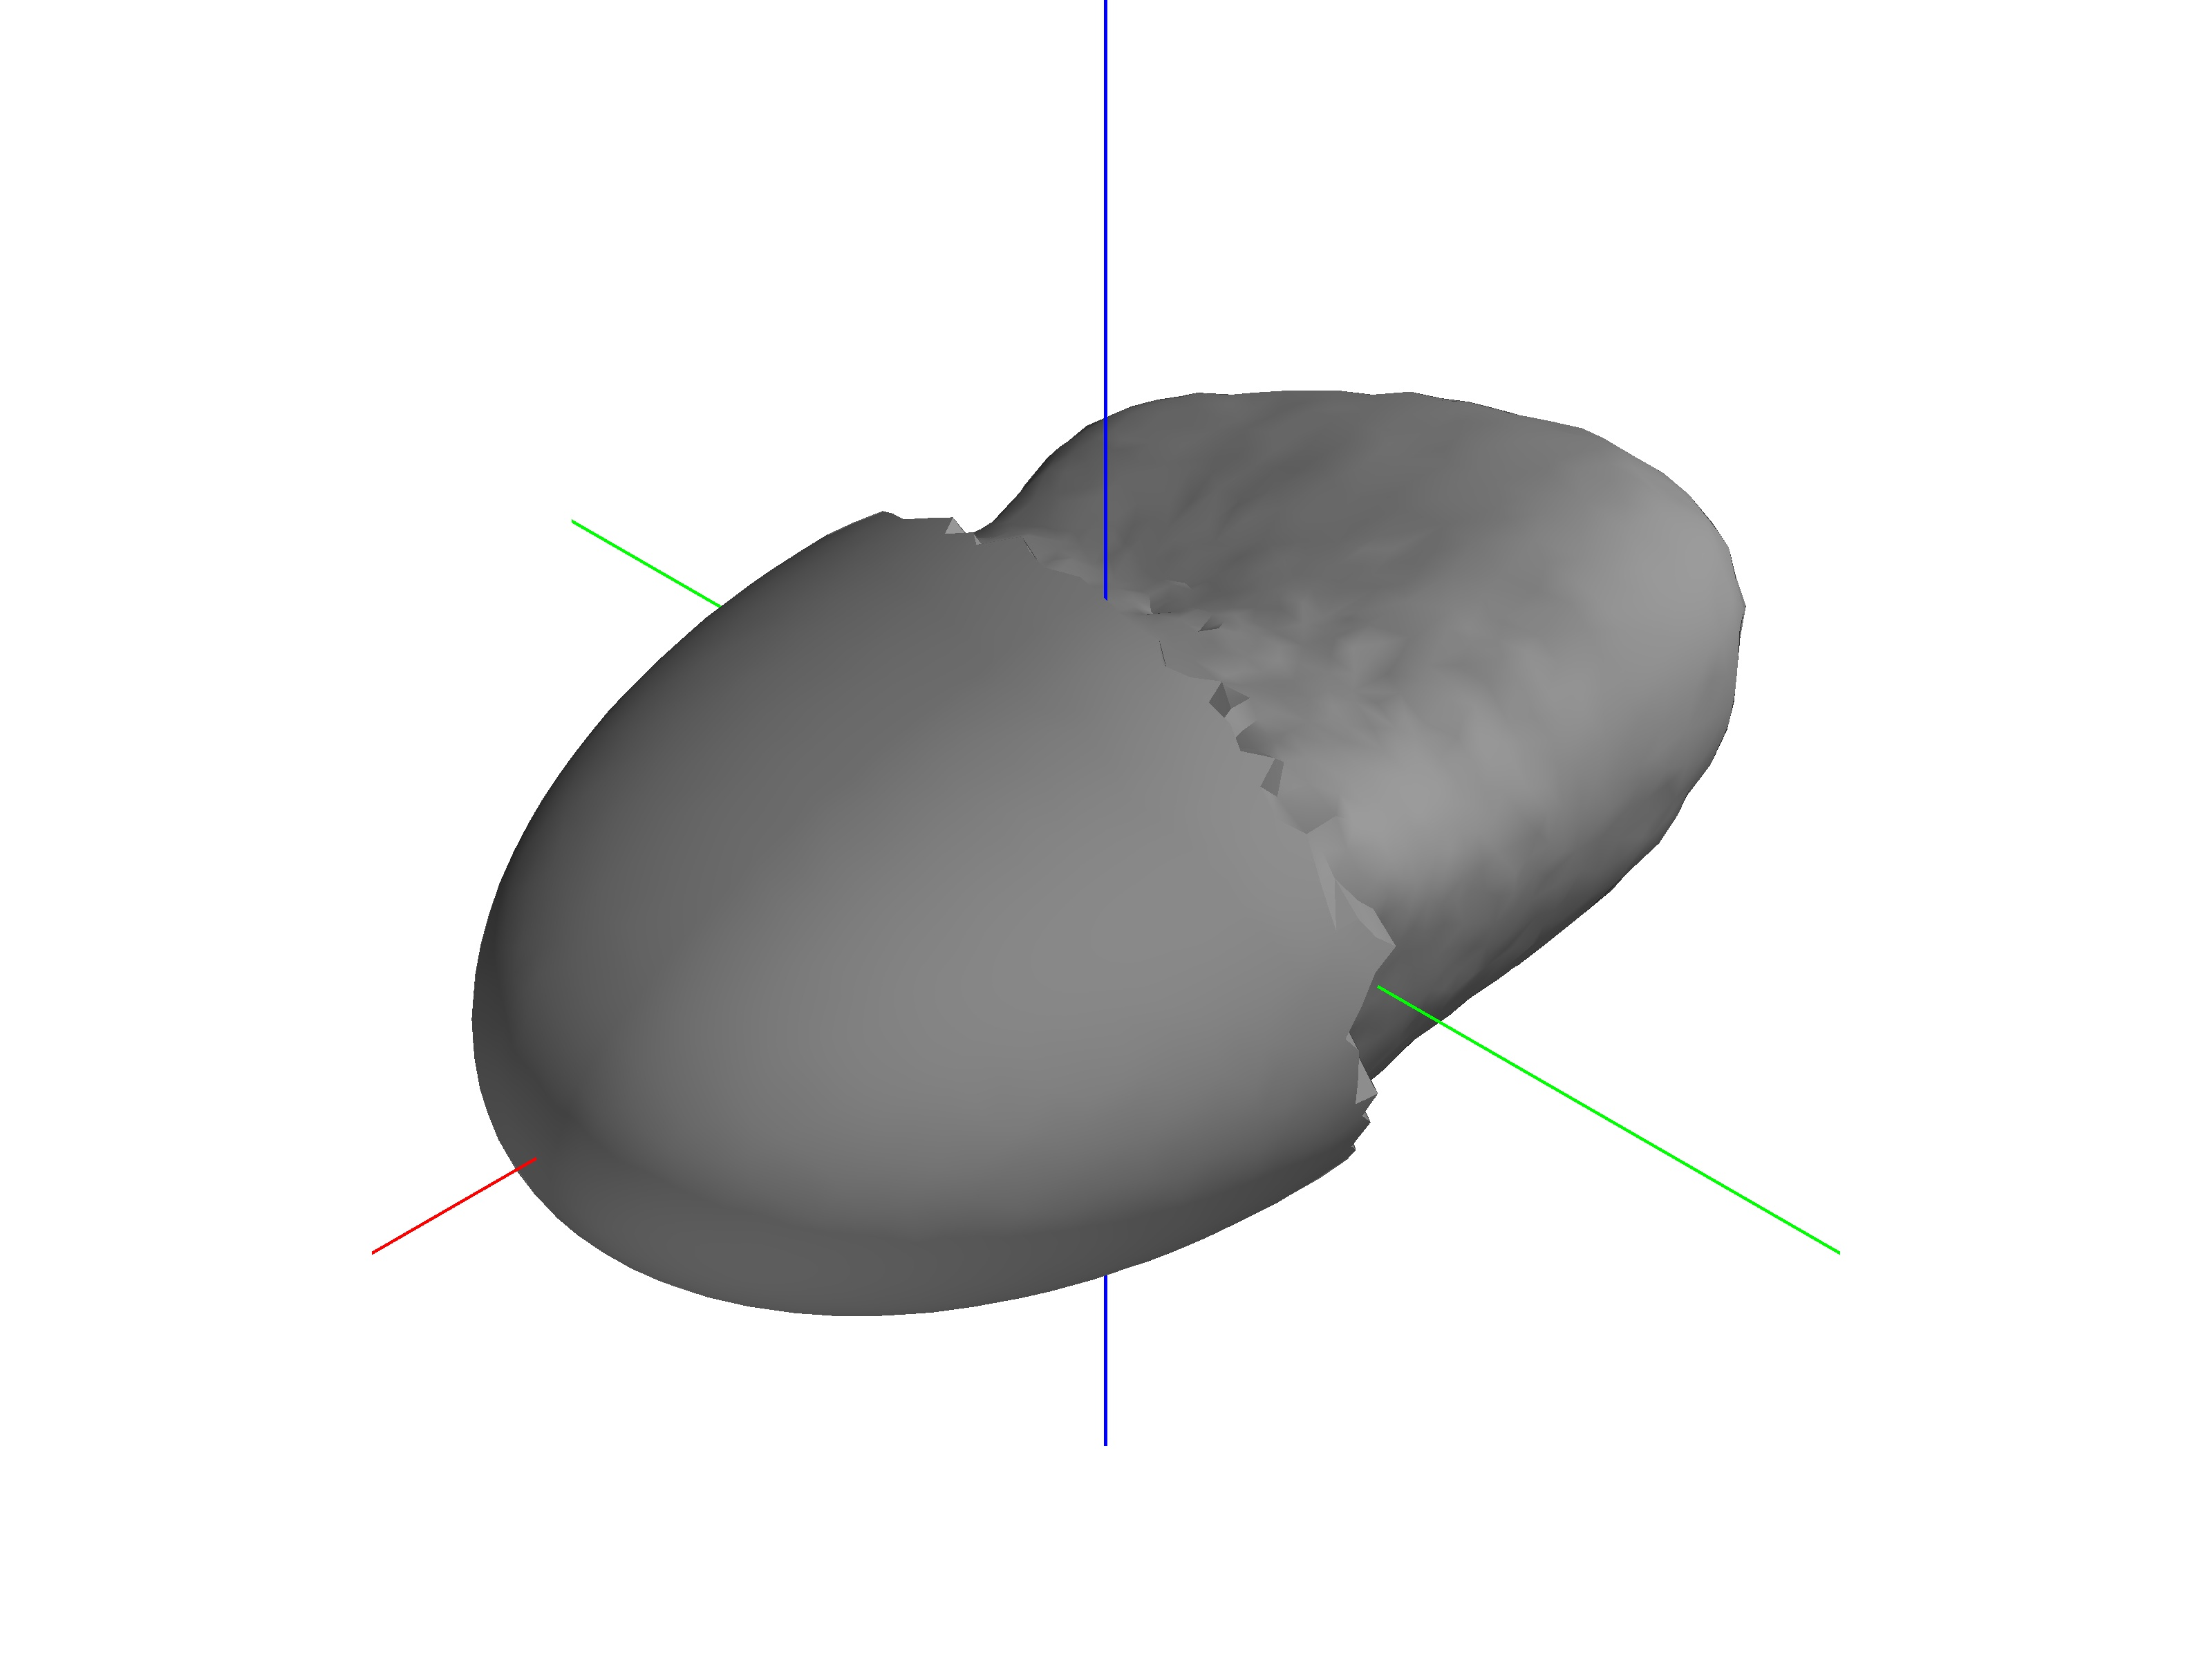
\includegraphics[width=0.5\textwidth]{figures/2018_SSPI/partial_1024.jpg}}

    \subcaptionbox{\SI{75}{\percent} of measurements added\label{fig:threequarter}}{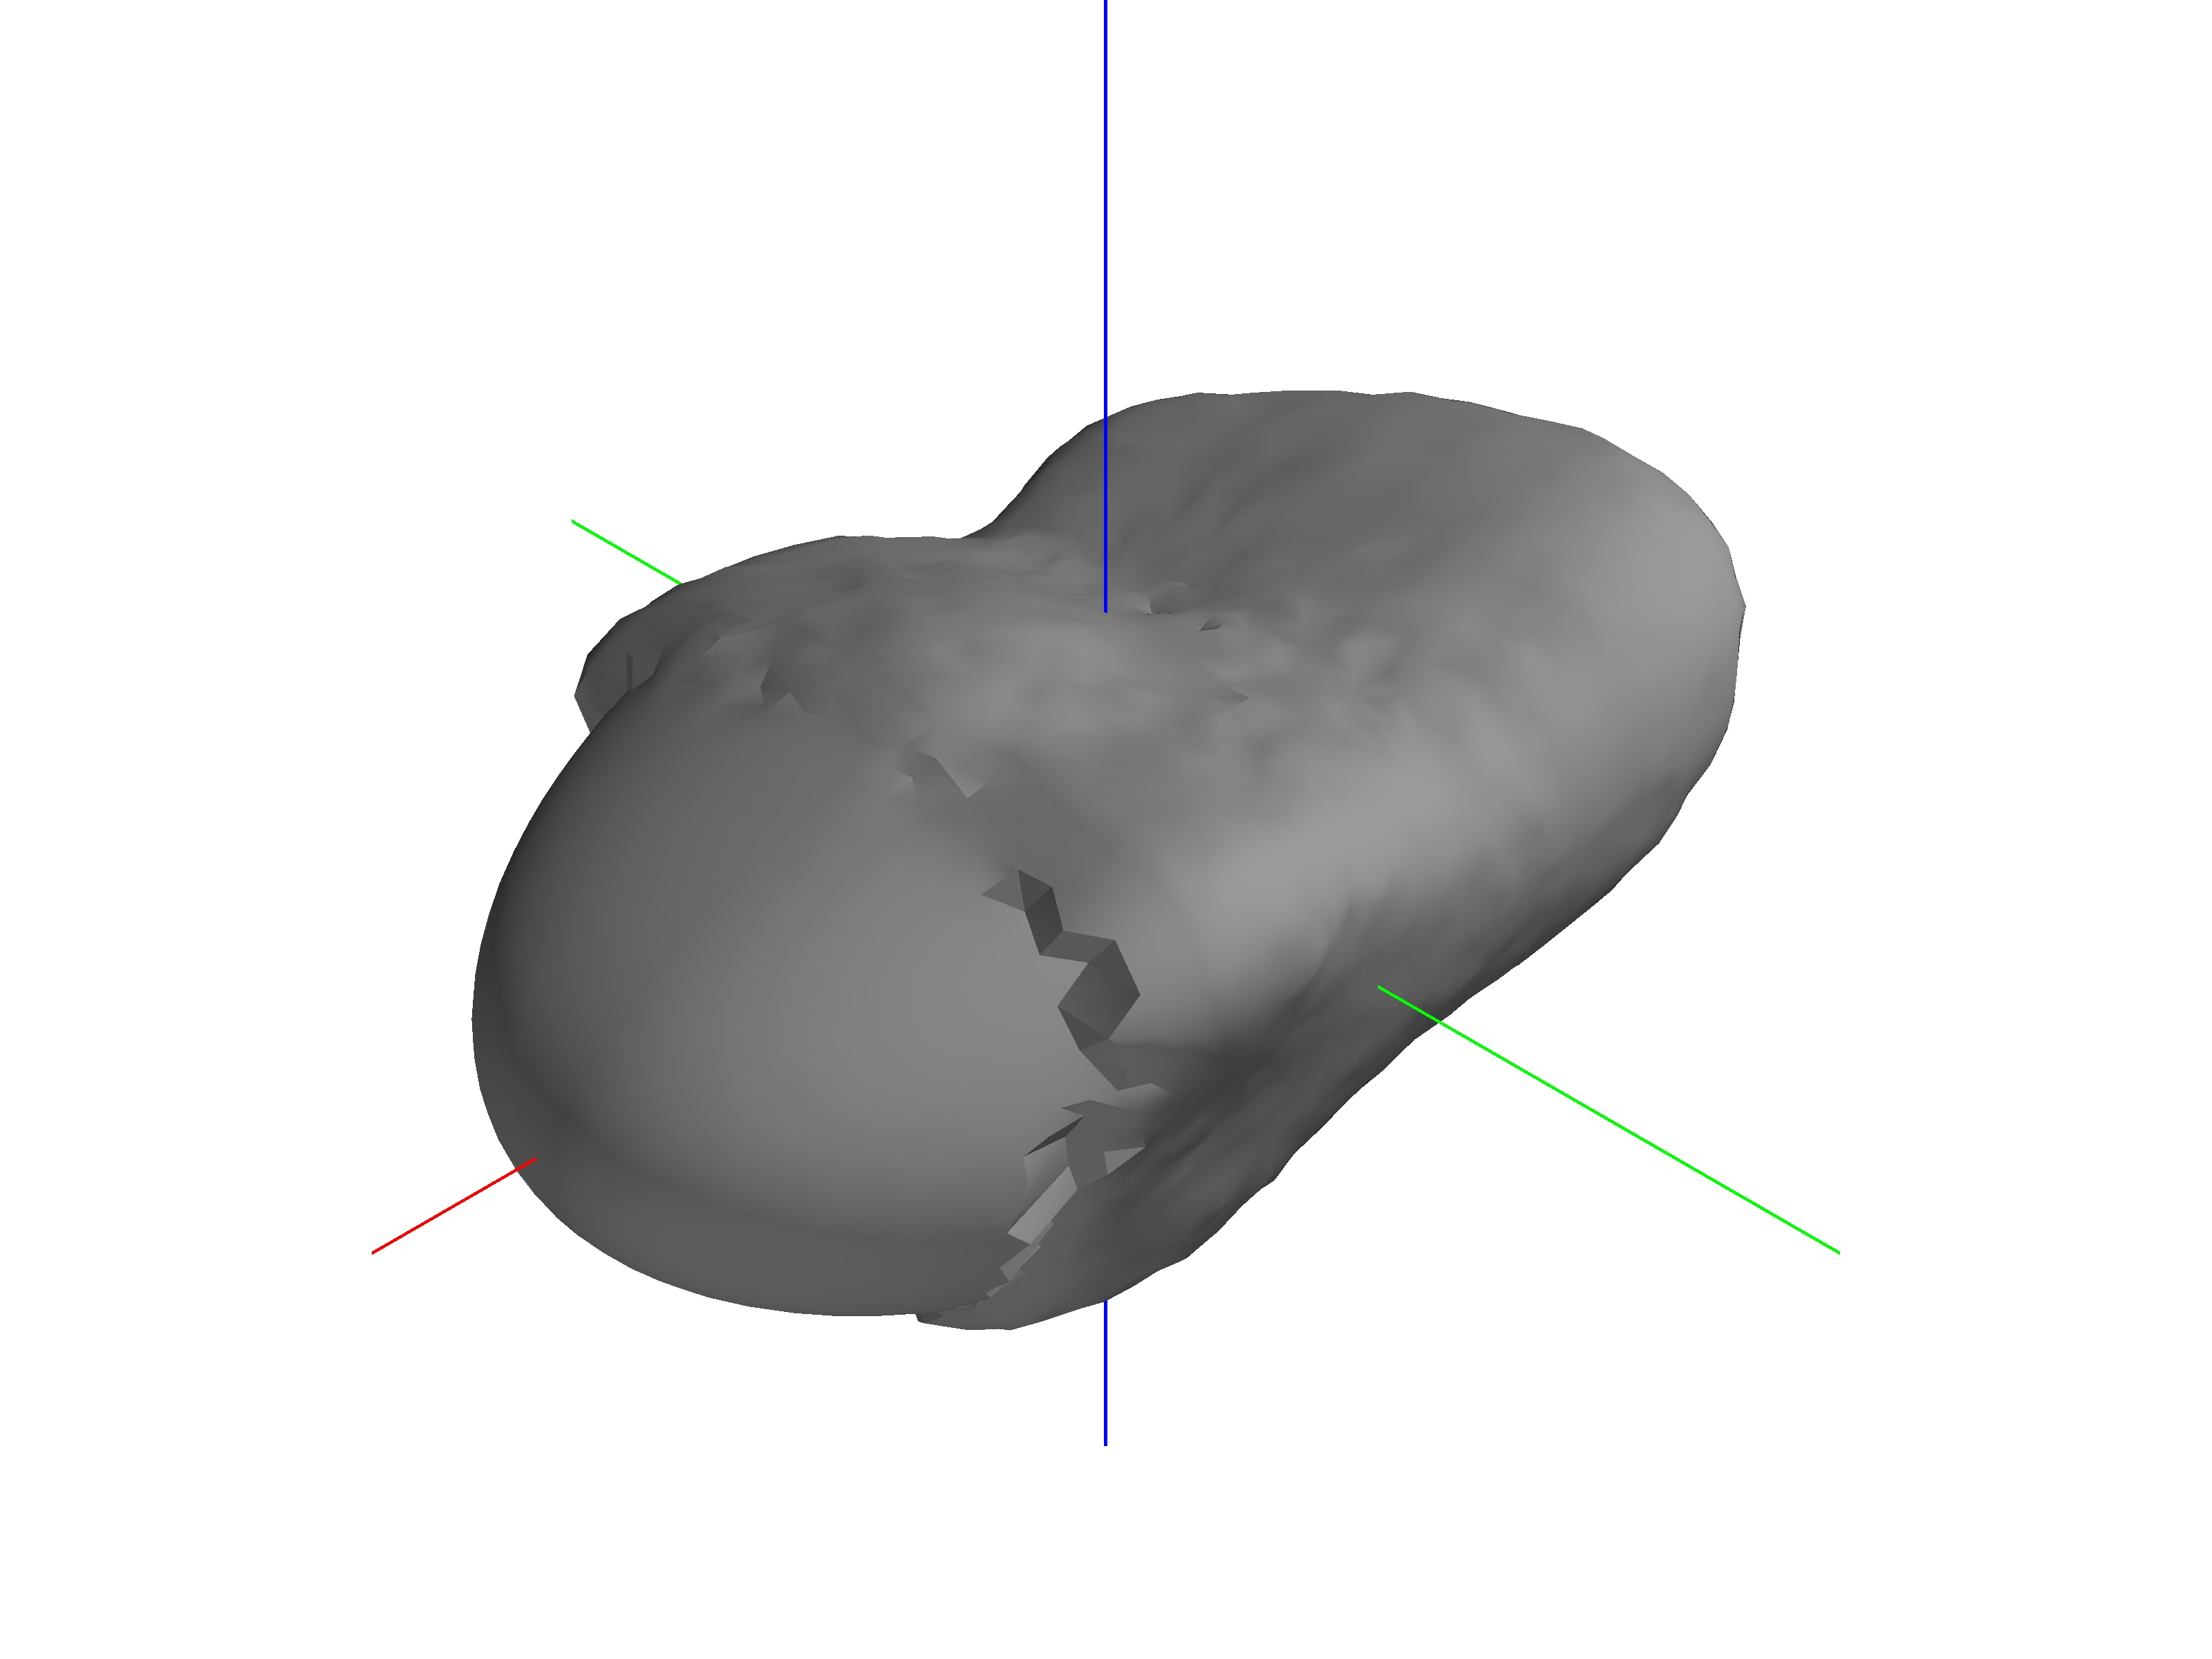
\includegraphics[width=0.5\textwidth]{figures/2018_SSPI/partial_1536.jpg}}~
    \subcaptionbox{Final reconstruction\label{fig:final}}{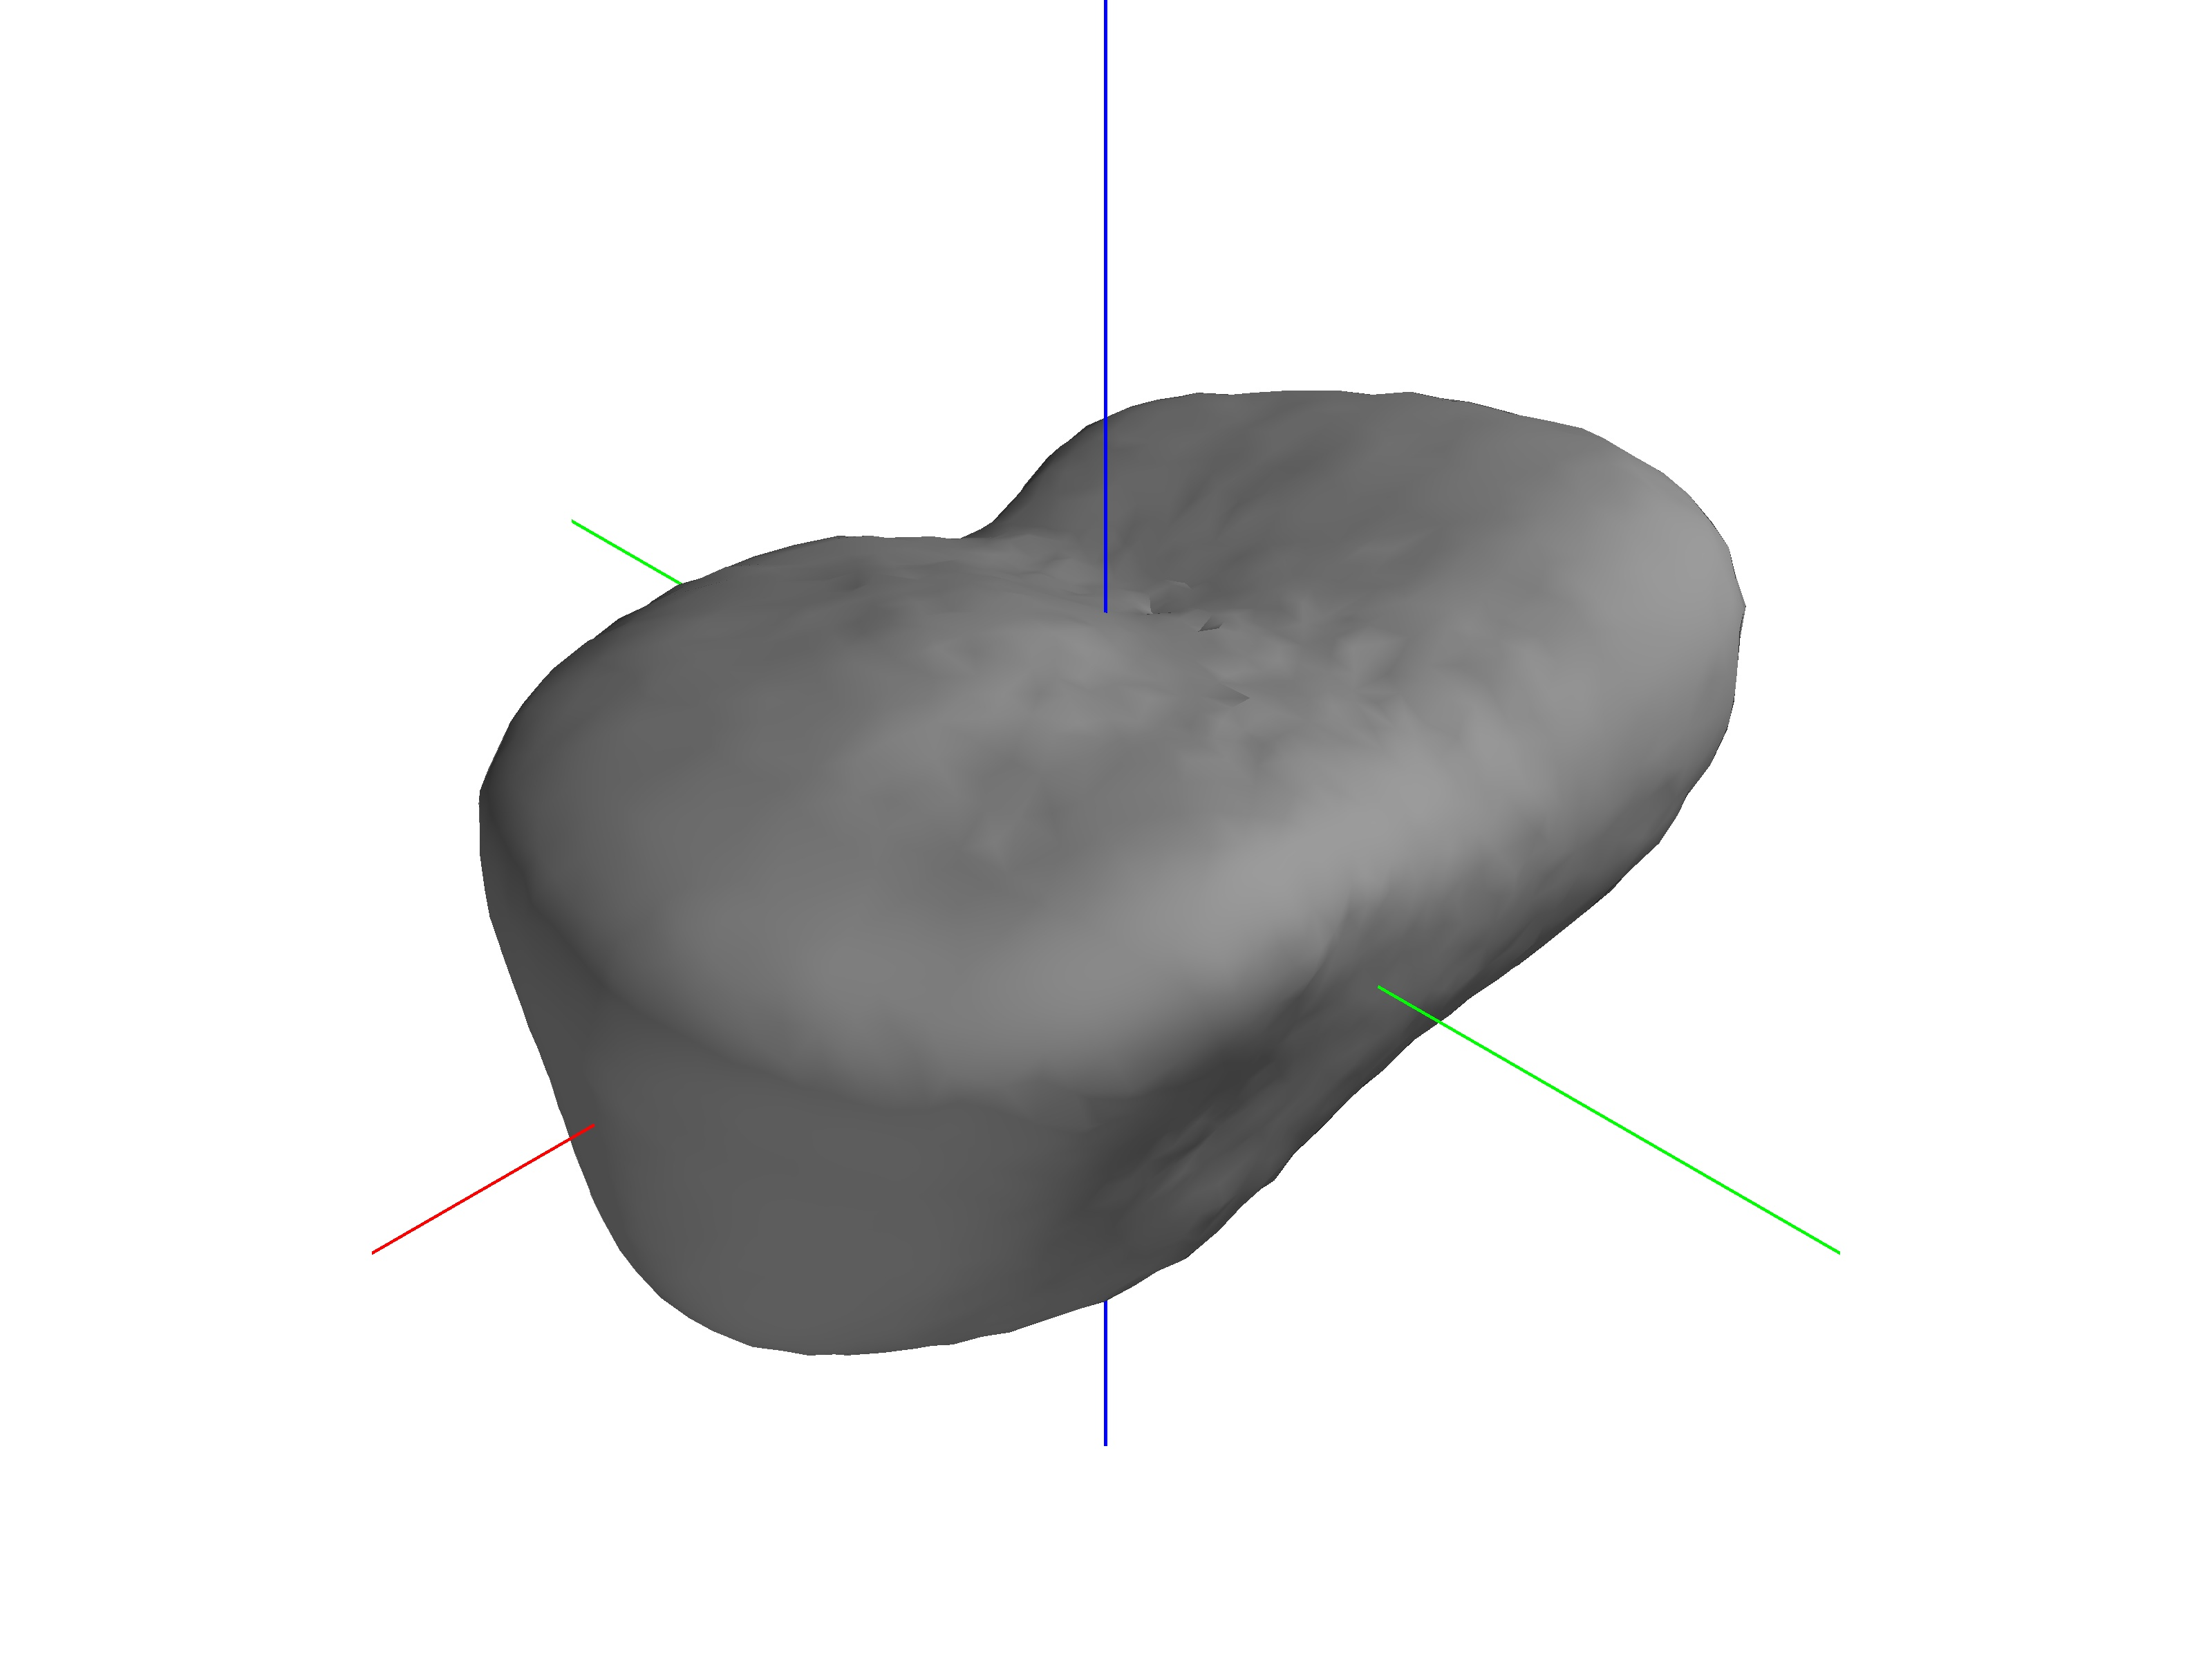
\includegraphics[width=0.5\textwidth]{figures/2018_SSPI/partial_2047.jpg}}
    \caption{4769 Castalia incremental reconstruction. The initial ellipsoid is incrementally modified by radially moving each vertex to best match the measurements.~\label{fig:reconstruction}}
\end{figure}
\section{Autonomous Mapping Guidance}\label{sec:explore_asteroid}

The mesh update algorithm presented in~\cref{sec:radius_update} does not offer a method to determine which portion of the surface needs to be updated. 
In this section, we present a computationally efficient approach to surface mapping and trajectory generation.
Utilizing the nonlinear controllers developed in~\cref{sec:se3_control} allows the spacecraft to manuever to the best location that will update the shape estimate.
Utilizing this approach enables autonomous operations at the asteroid. 

The ideal guidance approach involves solving a global optimal control problem which satisfies the system dynamics from~\cref{sec:dumbbell_model} while minimizing the shape uncertainty.
There are a wide variety of optimal control techniques which may be utilized to solve the problem, such as indirect methods~\cite{kirk2012,bryson1975}.
However, regardless of the method an optimal control formulation will result in a more computationally demanding algorithm.
Since the \gls{lidar} will be operating at upwards of \SI{1}{\hertz} efficient processing of the measurement and computation of the guidance commands is critical.

We define a cost associated with each vertex \( \vc{v}_i \) of the shape estimateas
\begin{align}\label{eq:explore_cost}
    J_i (\ipos) = \alpha_w J_{w_i} + \alpha_d J_{d_i}(\ipos) + \alpha_c J_{c_i}(\ipos)
\end{align}
where the weighting factors \( \alpha_w, \alpha_d, \alpha_c \in \R^1 \) are chosen such that \( \alpha_w + \alpha_d + \alpha_c = 1 \).
The term \( J_{w_i} \in \R^1 \) represents the cost associated with the uncertainty of vertex \( i \) as
\begin{align}\label{eq:weight_cost}
    J_{w_i} &= - \frac{w_i}{w_m}
\end{align}
where \( w_i \) is the uncertainty of vertex \( i \) and \( w_m \) is a maximum uncertainty used to scale the values.
The term \( J_{d_i} \) represents the scaled geodesic distance between the current state of the spacecraft and vertex \( i \),
\begin{align}\label{eq:distance_cost}
    J_{d_i}(\ipos) &= \frac{1}{\pi} \arctan \parenth{ \frac{\norm{\ipos \times \vc{v}_i}}{\ipos \cdot \vc{v}_i}}.
\end{align}

Finally, a control component is included in the cost function which penalizes vertices that are difficult to reach.
Consider, the current position of the spacecraft in the asteroid fixed frame as \( \rpos\) and a desired vertex \( \vc{v}_i \) of the shape estimate.
We can define a normal vector to the plane spanned by \( \rpos, \vc{v}_i \) as
\begin{align}\label{eq:normal_to_plane}
    \vc{n}_i = \frac{\rpos \times \vc{v}_i}{\norm{\rpos} \norm{\vc{v}_i}}.
\end{align}
Then a trajectory \( x_d(\theta) \) as
\begin{align}\label{eq:spherical_waypoint}
    x_d(\theta) = r_d \exp{\parenth{\theta \hat{\vc{n}_i}} } \frac{\rpos}{\norm{\rpos}},
\end{align}
where \( \theta : \bracket{0, \frac{\rpos \cdot \vc{v}_i}{\norm{\rpos}\norm{\vc{v}_i}}} \to \R^1\) parameterizes the desired trajectory.
\Cref{eq:spherical_waypoint} simply describes a portion of a great circle trajectory between the current state, \( \rpos \), and the desired vertex \( \vc{v}_i \)~\cite{chen2016}.
The altitude of the spacecraft, \( r_d \in \R \), can be chosen based on sensor characterisitics of safety concerns.
For example, \( r_d \) can be chosen as the distance of the Biroullin sphere with an additional safety margin to mitigate any surface collision.
The translational controller presented in~\cref{eq:translational_control} is used to determine the magnitude of the control to follow \( x_d\).
We assume that the tracking errors are small, such that \( e_x, e_v \) are negligible, therefore the control becomes
\begin{align}\label{eq:tracking_control_cost}
    u_f(\theta) = -F_{ext}(x_d(\theta)), 
\end{align}
where the external force is defined by the polyhedron potential model given in~\cref{eq:inertial_velocity_dynamics}.
The control cost is then defined as the integral over the desired trajectory~\cref{eq:spherical_waypoint} between the current state and the desired vertex as
\begin{align}\label{eq:control_cost}
    J_{c_i}(\rpos) = \frac{1}{u_m} \int_{\theta_0}^{\theta_f} u_f(\theta)^T R u_f(\theta) d\theta,
\end{align}
where \( u_m \) is used to normalize and scale \( J_{c_i} \).
\Cref{eq:control_cost} is numerically integrated over the trajectory \( x_d(t) \) and used to penalize vertices which have a larger cost.

The vertex which minimizes~\cref{eq:explore_cost} 
\begin{align*}
    \vc{v}_{min} = \min_{\vc{v}_i} J,
\end{align*}
is determined and used to determine the desired position of the spacecraft in the asteroid fixed frame.
The terminal state is transformed into the inertial frame and chosen as a point above \( \vc{v}_{min} \) as
\begin{align}
    \rpos = r_d \aatt \vc{v}_{min}, 
\end{align}
where \( r_d \) is again chosen to ensure a safety margin above the surface.
The desired attitude command, \( R_d\), is chosen such that the spacecraft camera axis, \( \vc{b}_1 \), is directed along the nadir towards the asteroid.
It is sufficient to define two orthogonal vectors to uniquely determine the attitude of the spacecraft.
The \( \vc{b}_{3d} \) vector is chosen to lie in the plane spanned by \(\vc{b}_{1d} \) and \( \vc{e}_3 = \vc{f}_3 \).
The desired attitude command is defined as
\begin{align}
    \vc{b}_{1d} &= - \frac{\vc{x}}{\norm{\vc{x}}} , \\
    \vc{b}_{3d} &= \frac{\vc{f}_3 - \parenth{\vc{f}_3 \cdot \vc{b}_{1d}} \vc{b}_{1d}}{\norm{\vc{f}_3 - \parenth{\vc{f}_3 \cdot \vc{b}_{1d}} \vc{b}_{1d}}}, \\
    \vc{b}_{2d} &= \vc{b}_{3d} \times \vc{b}_{1d} , \\
    R_d &= \begin{bmatrix} \vc{b}_{1d} & \vc{b}_{2d} & \vc{b}_{3d} \end{bmatrix} .
\end{align}
The camera axis is aligned with the spacecraft \( \vb{b}_ 1 \) axis, which is direted towards the asteroid, throughout the trajectory.

\subsection{Landing Area Refinement}\label{sec:landing_refinement}
The shape update approach presented in~\cref{sec:radius_update} is designed with autonomous operations in mind. 
It is based on an initial coarse shape estimate that is iteratively updated with range measurements of the surface.
Furthermore, the original mesh is uniformly distributed and as a result many small topological features such as rocks or small craters are not be captured by the shape model. 
However, these small features are critical for surface operations and safe landings.
In addition, it would be computationaly prohibitive to have a uniformly high resolution mesh.
In this section, we extend the previous shape update approach to enable a much higher fidelity in a specific location.

Mixed resolution surface meshes are routinely used in finite element and geometric modeling applications~\cite{botsch2010}.
As shown in~\cite{mcmahon2017}, utilizing mixed resolution shape models for asteroid missions offers the potential of reduced computational demands.
The computational cost of the polyhedron potential model given by~\cref{eq:potential} is roughly proporitional to the number of faces in the shape model.
As a result, a uniformly high resolution shape would quickly become intractable for realtime operations.
However, utilizing a mixed resolution approach allows for a high fidelity in a smaller mission critical area, such as a landing site, with a limited impact on the computational cost.

The selection of a landing site will typically require a vast quantity of data and weigh a multitude of possible metrics, such as scientific value, hardware constraints, timing and communication limits, or safety considerations. 
In our analysis we consider the surface slope, the distance to the surface, and a fictitious science metric in order to determine the best landing site based on the complete shape estimate.
This approach allows for a spacecraft to autonomously select and land on an asteroid.

The surface slope is computed according to the method developed in~\cite{scheeres1996}.
Due to the small size, and therefore low gravitational attraction, the force at each point on the surface is a combination of the gravitational attraction and the centripital acceleration.
At the center of each face, \( f_i = \begin{bmatrix} f_x & f_y & f_z \end{bmatrix} \), we compute a modified surface acceleration as
\begin{align}\label{eq:surface_force}
    U_m = \omega^2 \begin{bmatrix} f_x \\ f_y \\ 0 \end{bmatrix} + \begin{bmatrix} U_x \\ U_y \\ U_z \end{bmatrix},
\end{align}
where \( \omega \in \R^1 \) is the angular velocity of the asteroid and \( U_i \) is computed from~\cref{eq:attraction}.
Then the surface slope can be computed from
\begin{align}\label{eq:surface_slope}
    \cos \parenth{ \pi - \phi } = \frac{\vc{n}_f \cdot U_m}{\norm{U_m}},
\end{align}
where \( \phi \in \R^1 \) is the surface slope defines the angle between the surface normal \( \vc{n}_f \in \R^3 \) and the force vector at the surface.
If \( \phi = \SI{0}{\degree} \) then the force vector and the surface normal are anti-parallel, while \( \phi > \SI{90}{\degree} \) means that a particle on the surface would be thrown off the body as the centripetal force is larger than the gravitational attraction.

Additionally, we compute the distance, using~\cref{eq:geodesic_distance}, between the spacecraft state and each face of the asteroid. 
Finally, we also assign a random science value to the surface in the form of two dimensional Gaussian.
Utilizing these metric, a landing site is chosen to minimize the surface cost given as
\begin{align}\label{eq:surface_cost}
    J_l =  J_{\text{distance}} - J_{\text{science}},
\end{align}
where the surface slope is considered a hard constraint such that any candidate landing site must satisify \( \phi \leq \phi_m \).

\paragraph{Mesh Refinement}\label{sec:refinement}
Once a suitable landing site is selected the surround area is isolated and refined by adding new vertices and faces in the specified area.
The goal of refinement, or more generally remeshing, is given a mesh ( or a portion of it), compute another mesh whose elements satisfy some quality metrics while suitabably approximating the original mesh.
In this work, we utilize the isotropic remeshing algorithm implemented in \gls{cgal}.
This algorithm uses an iterative method which repeatedly splits long edges, collapses short edges, and relocates vertices until all edges are approximately the desired target edge length.
\begin{figure}[htbp]
    \centering
    \includegraphics[width=\textwidth]{example-image-golden}
    \caption[Isotropic Remeshing]{LOOK IN PMP 101 Local remeshing operations.(Image duplicated from~\cite{botsch2010})\label{fig:isotropic_remeshing}}
\end{figure}
For example,~\cref{fig:cube_remesh} shows the isotropic remeshing result for the selected faces of a unit cube.
The original unit cube is composed of \num{8} vertices and \num{12} faces.
The two triangular faces of the visible side of the cube are selected for the isotropic remeshing operation as shown in~\cref{fig:cube_original_mesh}.
A target edge length of \num{0.1} is selected for these faces and used to generate~\cref{fig:cube_refine_mesh}.
The two large triangular faces are divided into a number of smaller triangular faces.
Furtheremore, the addiitonal faces are all approximatley the same size and preserve the original surface of the cube.
After the isotropic remeshing operation the number of vertices has increased from \num{8} to \num{140}.
\begin{figure}[htbp]
    \centering
    \subcaptionbox{Original Cube\label{fig:cube_original_mesh}}{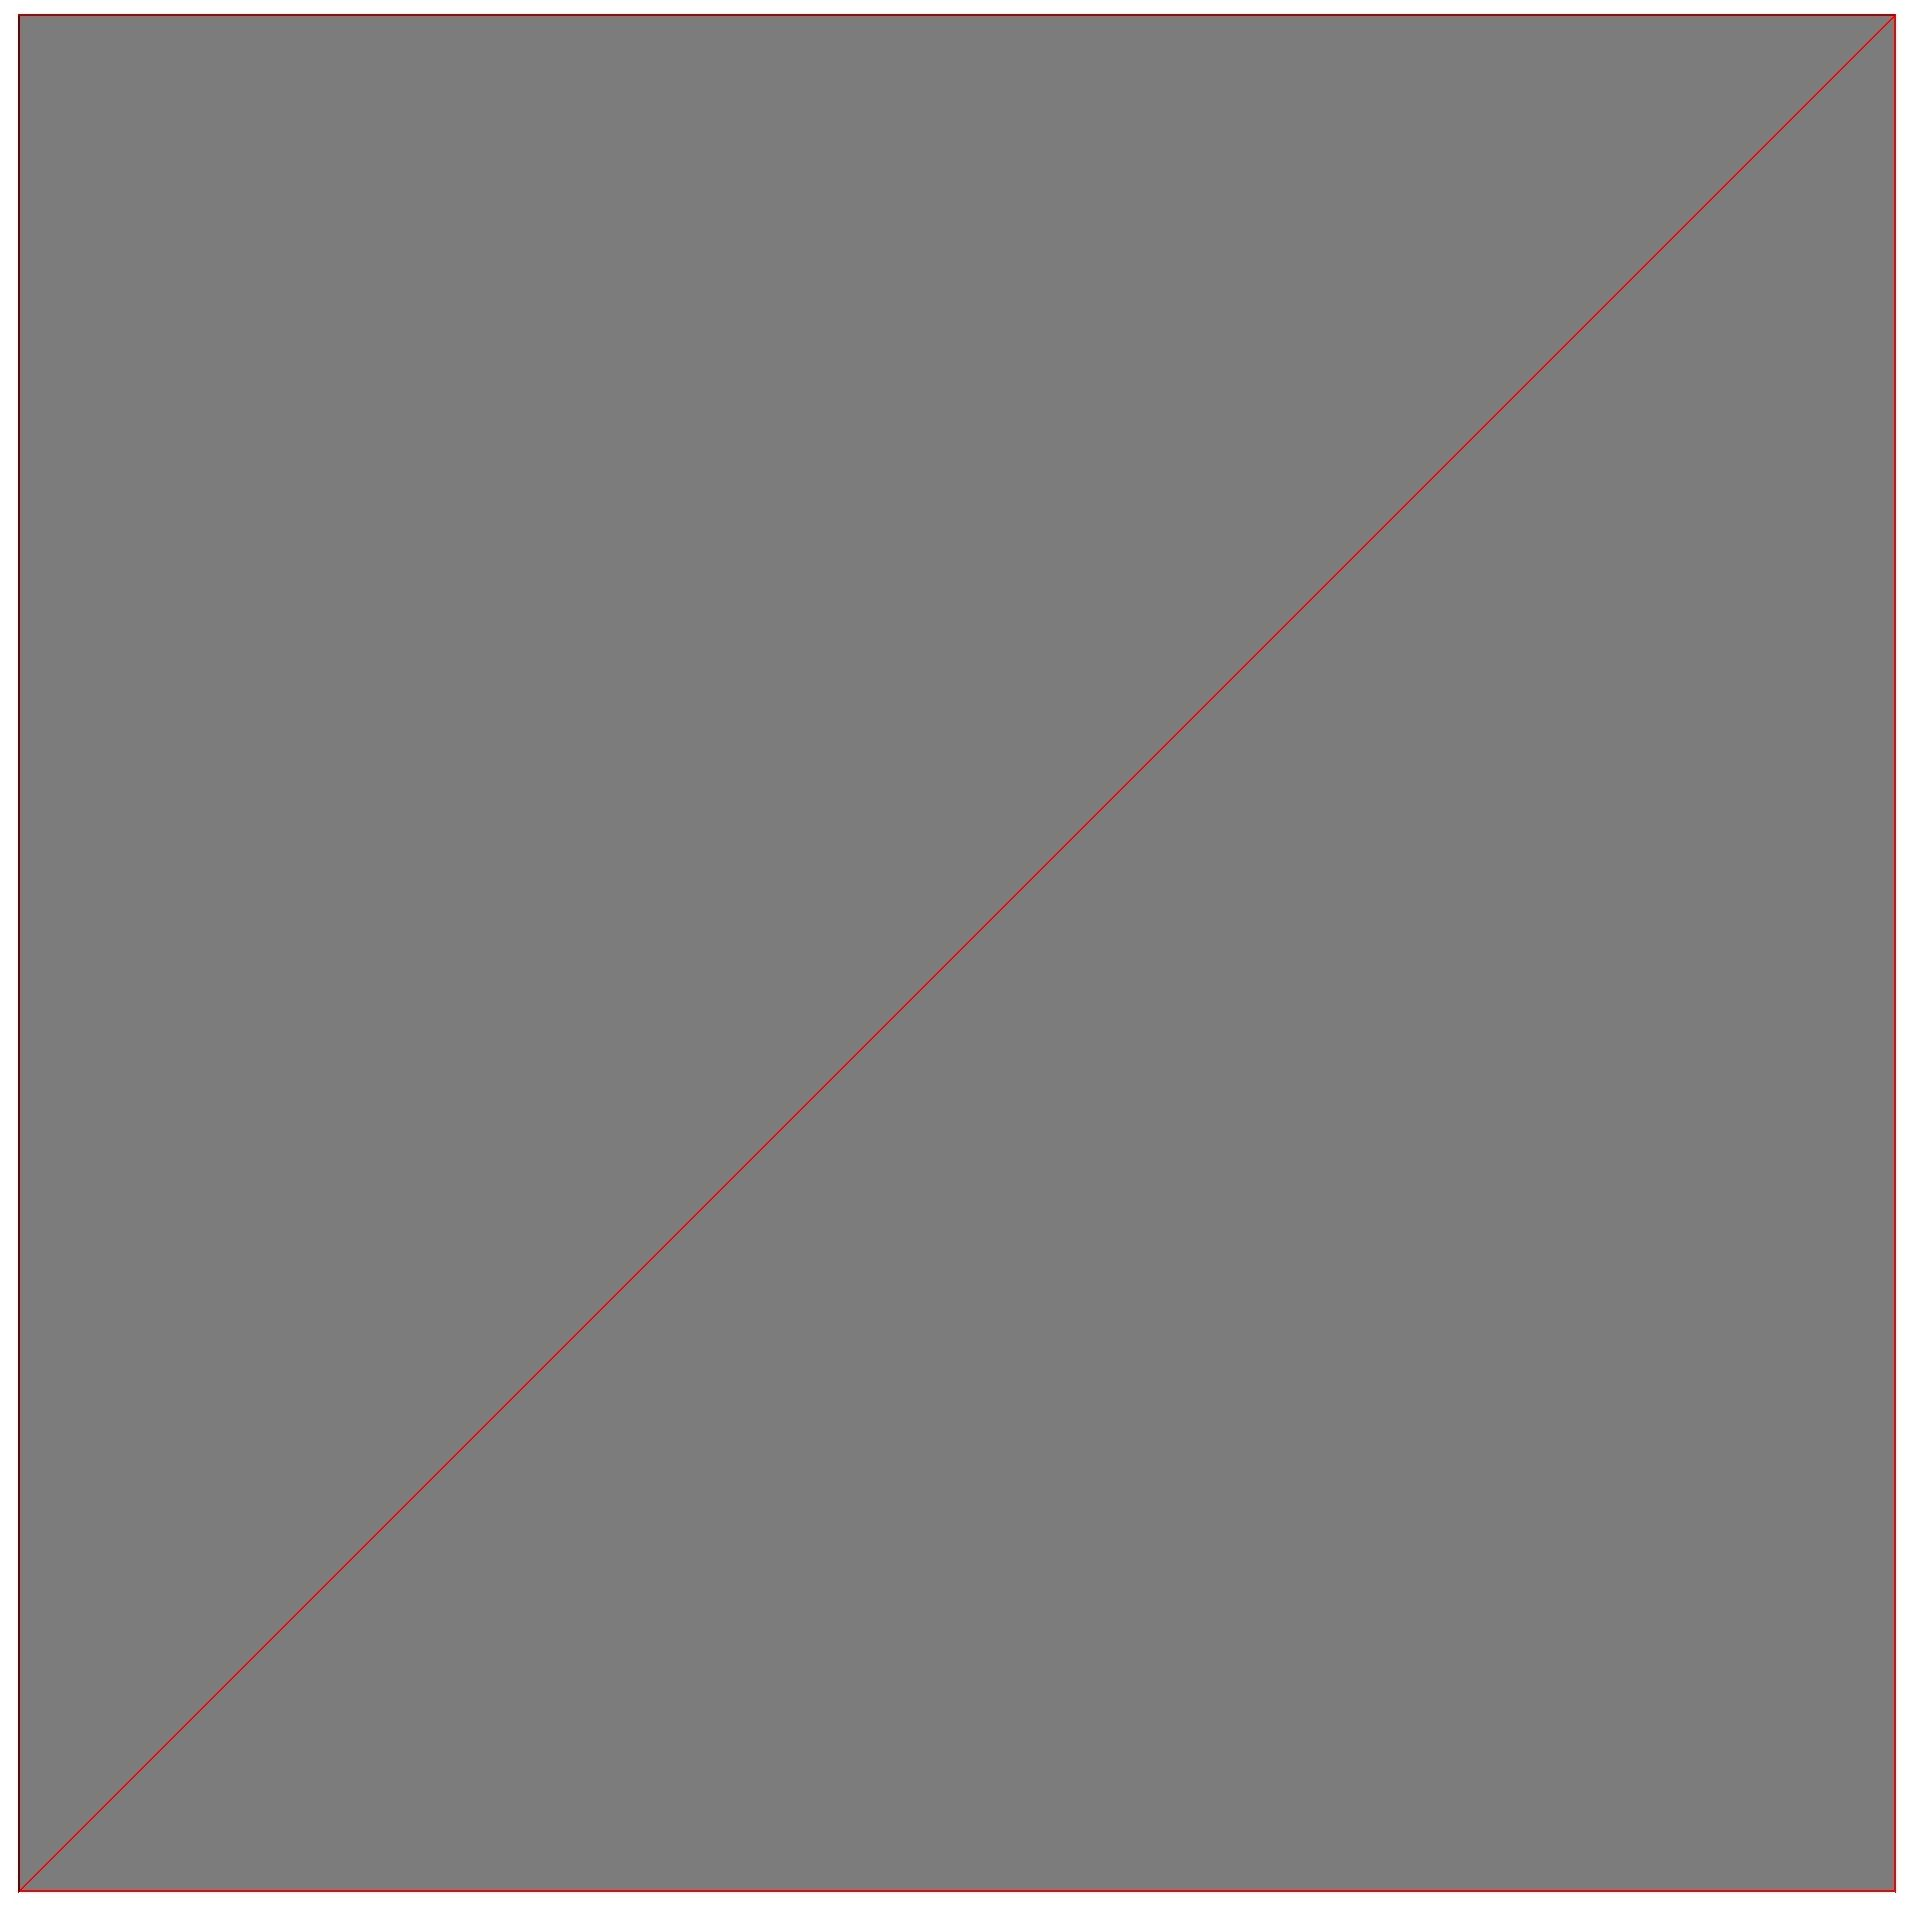
\includegraphics[width=0.5\textwidth]{figures/computational_geometry/isotropic/original_cube.jpg}}~
    \subcaptionbox{Remeshed Cube\label{fig:cube_refine_mesh}}{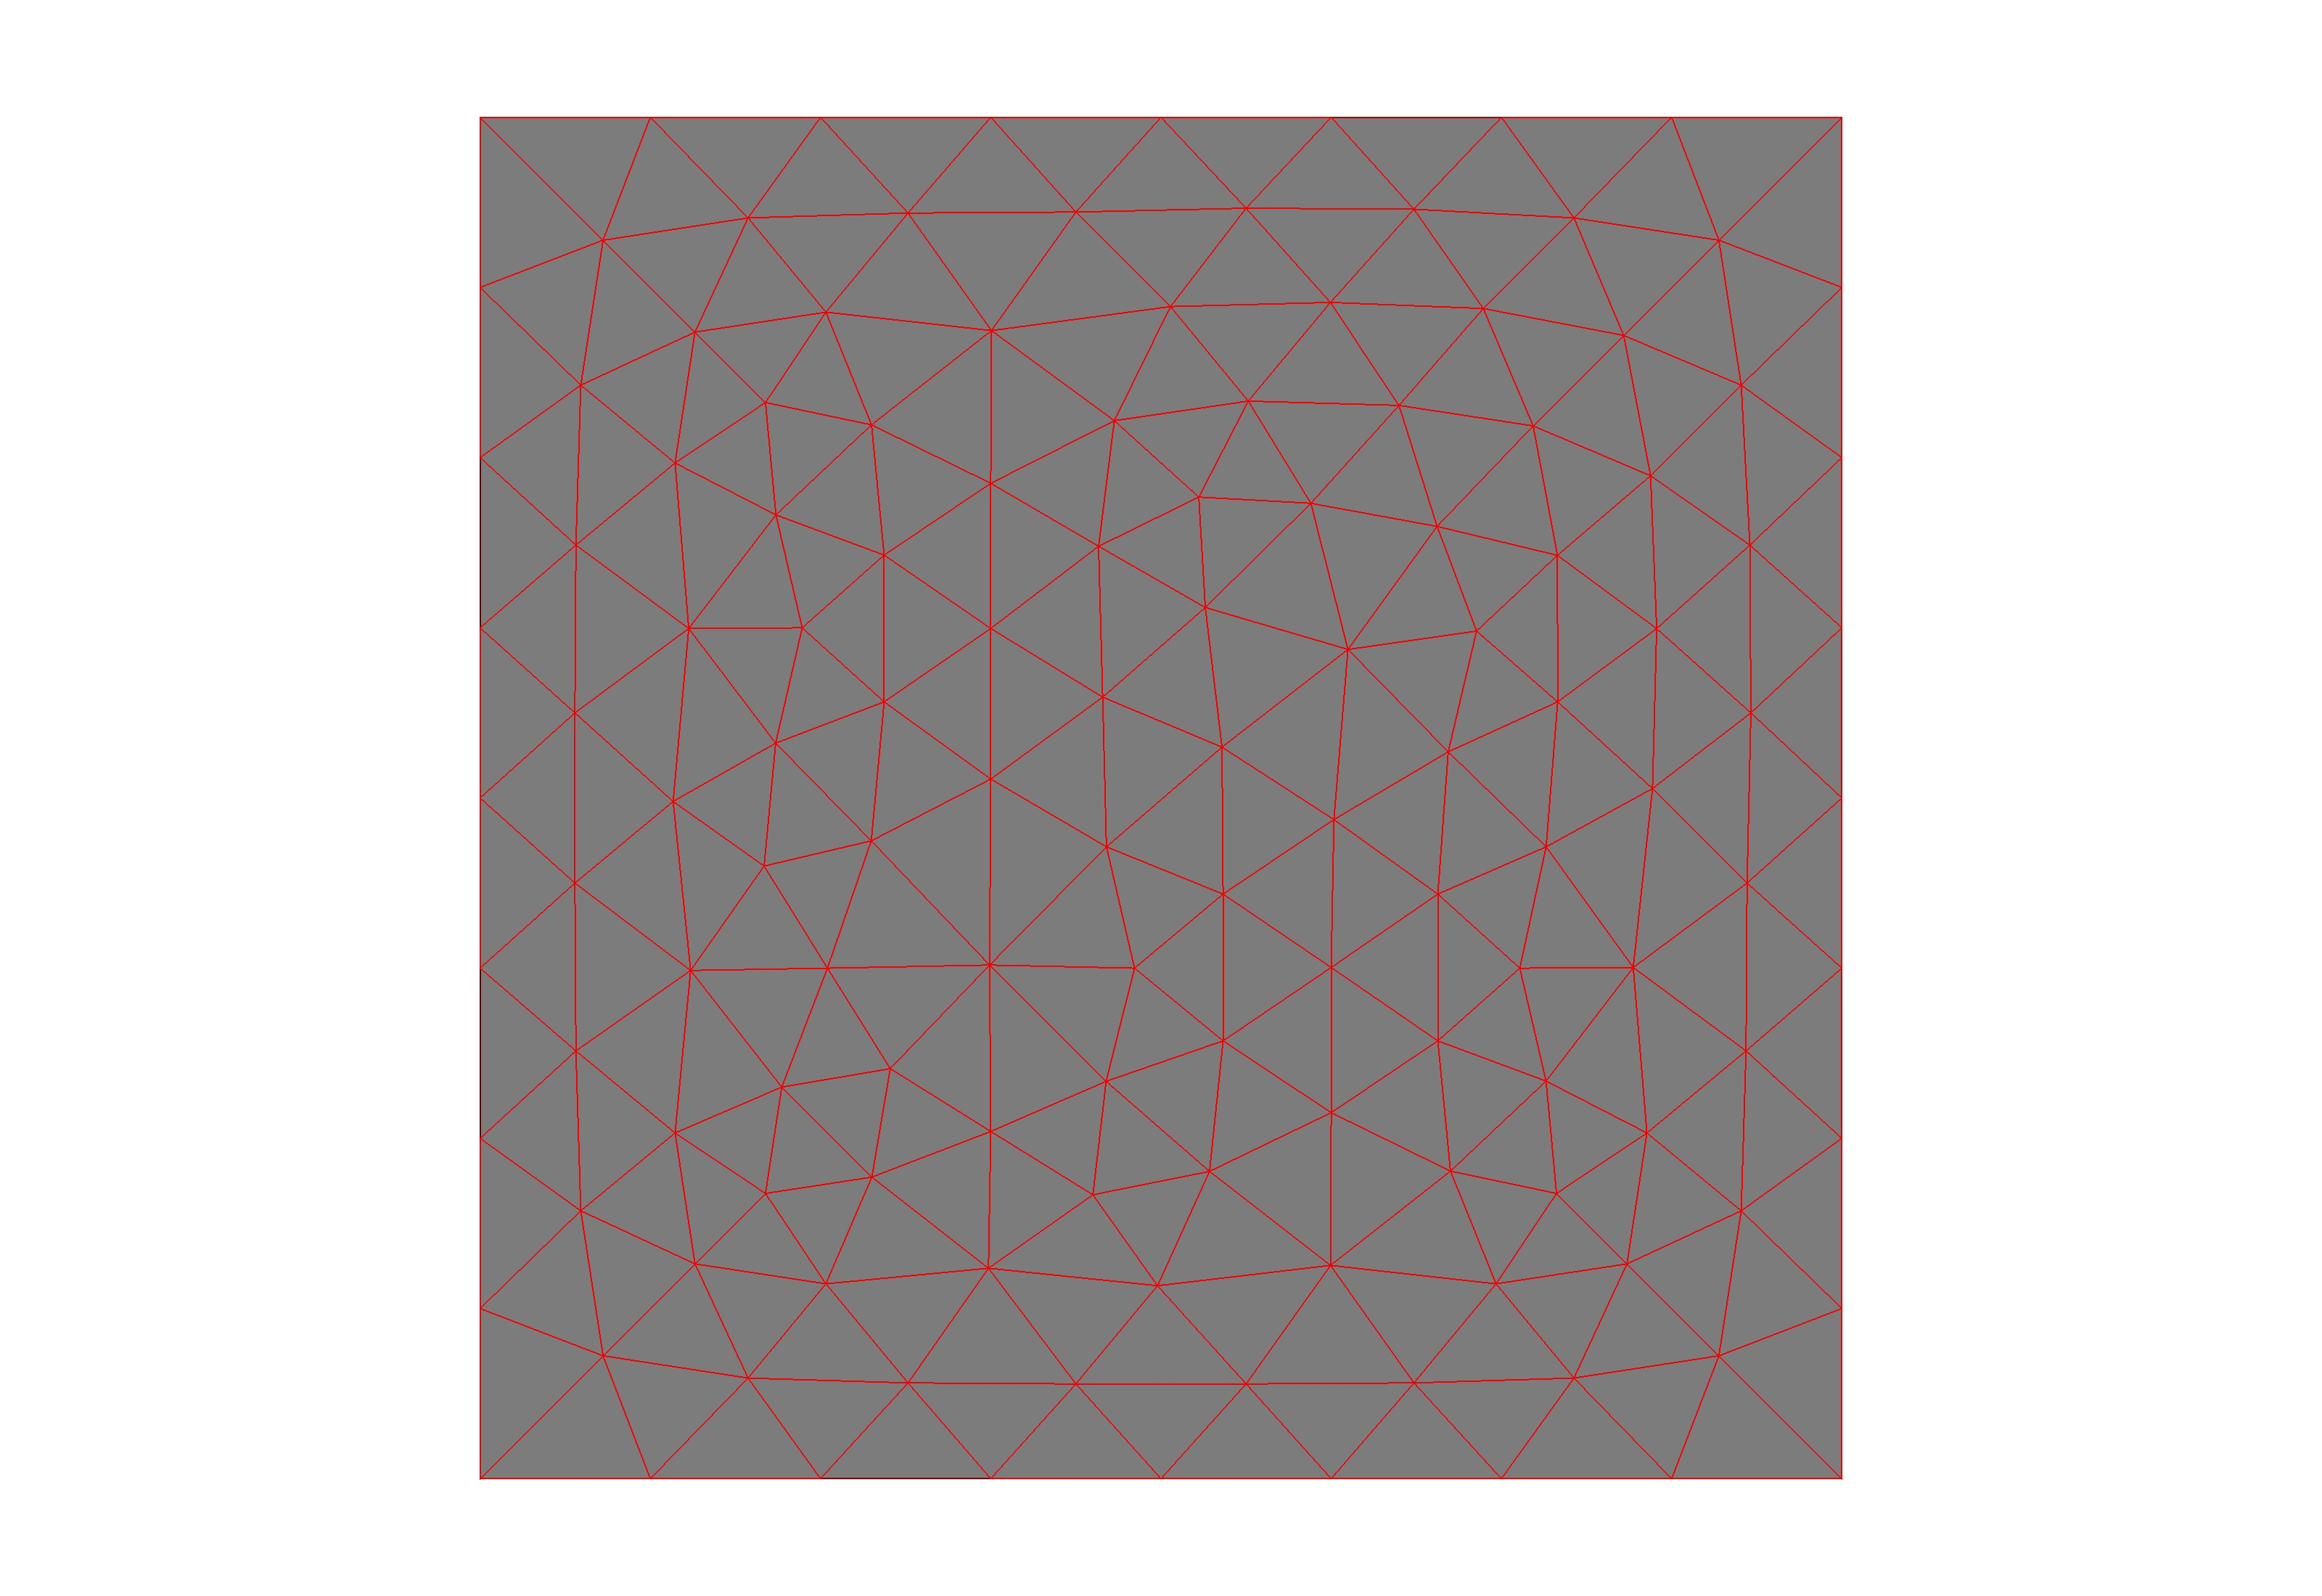
\includegraphics[width=0.5\textwidth]{figures/computational_geometry/isotropic/remesh_cube.jpg}}
    \caption{Example of Isotropic remeshing of a face of a cube\label{fig:cube_remesh}}
\end{figure}

The true shape model of asteroid Castalia is generated from radar imagery.
As a result, the shape model is not highly detailed as it does not contain small craters or surface features.
In order to apply the landing refinement process we agument a small portion of the mesh with some additional features and utilize the mesh update scheme in~\cref{sec:radius_update} to measure the surface.
The augmented model of Castalia is shown in~\cref{fig:bumpy_castalia}.
\begin{figure}[htbp]
    \centering
    \subcaptionbox{Augmented shape of Castalia with surface features\label{fig:orig_castalia}}{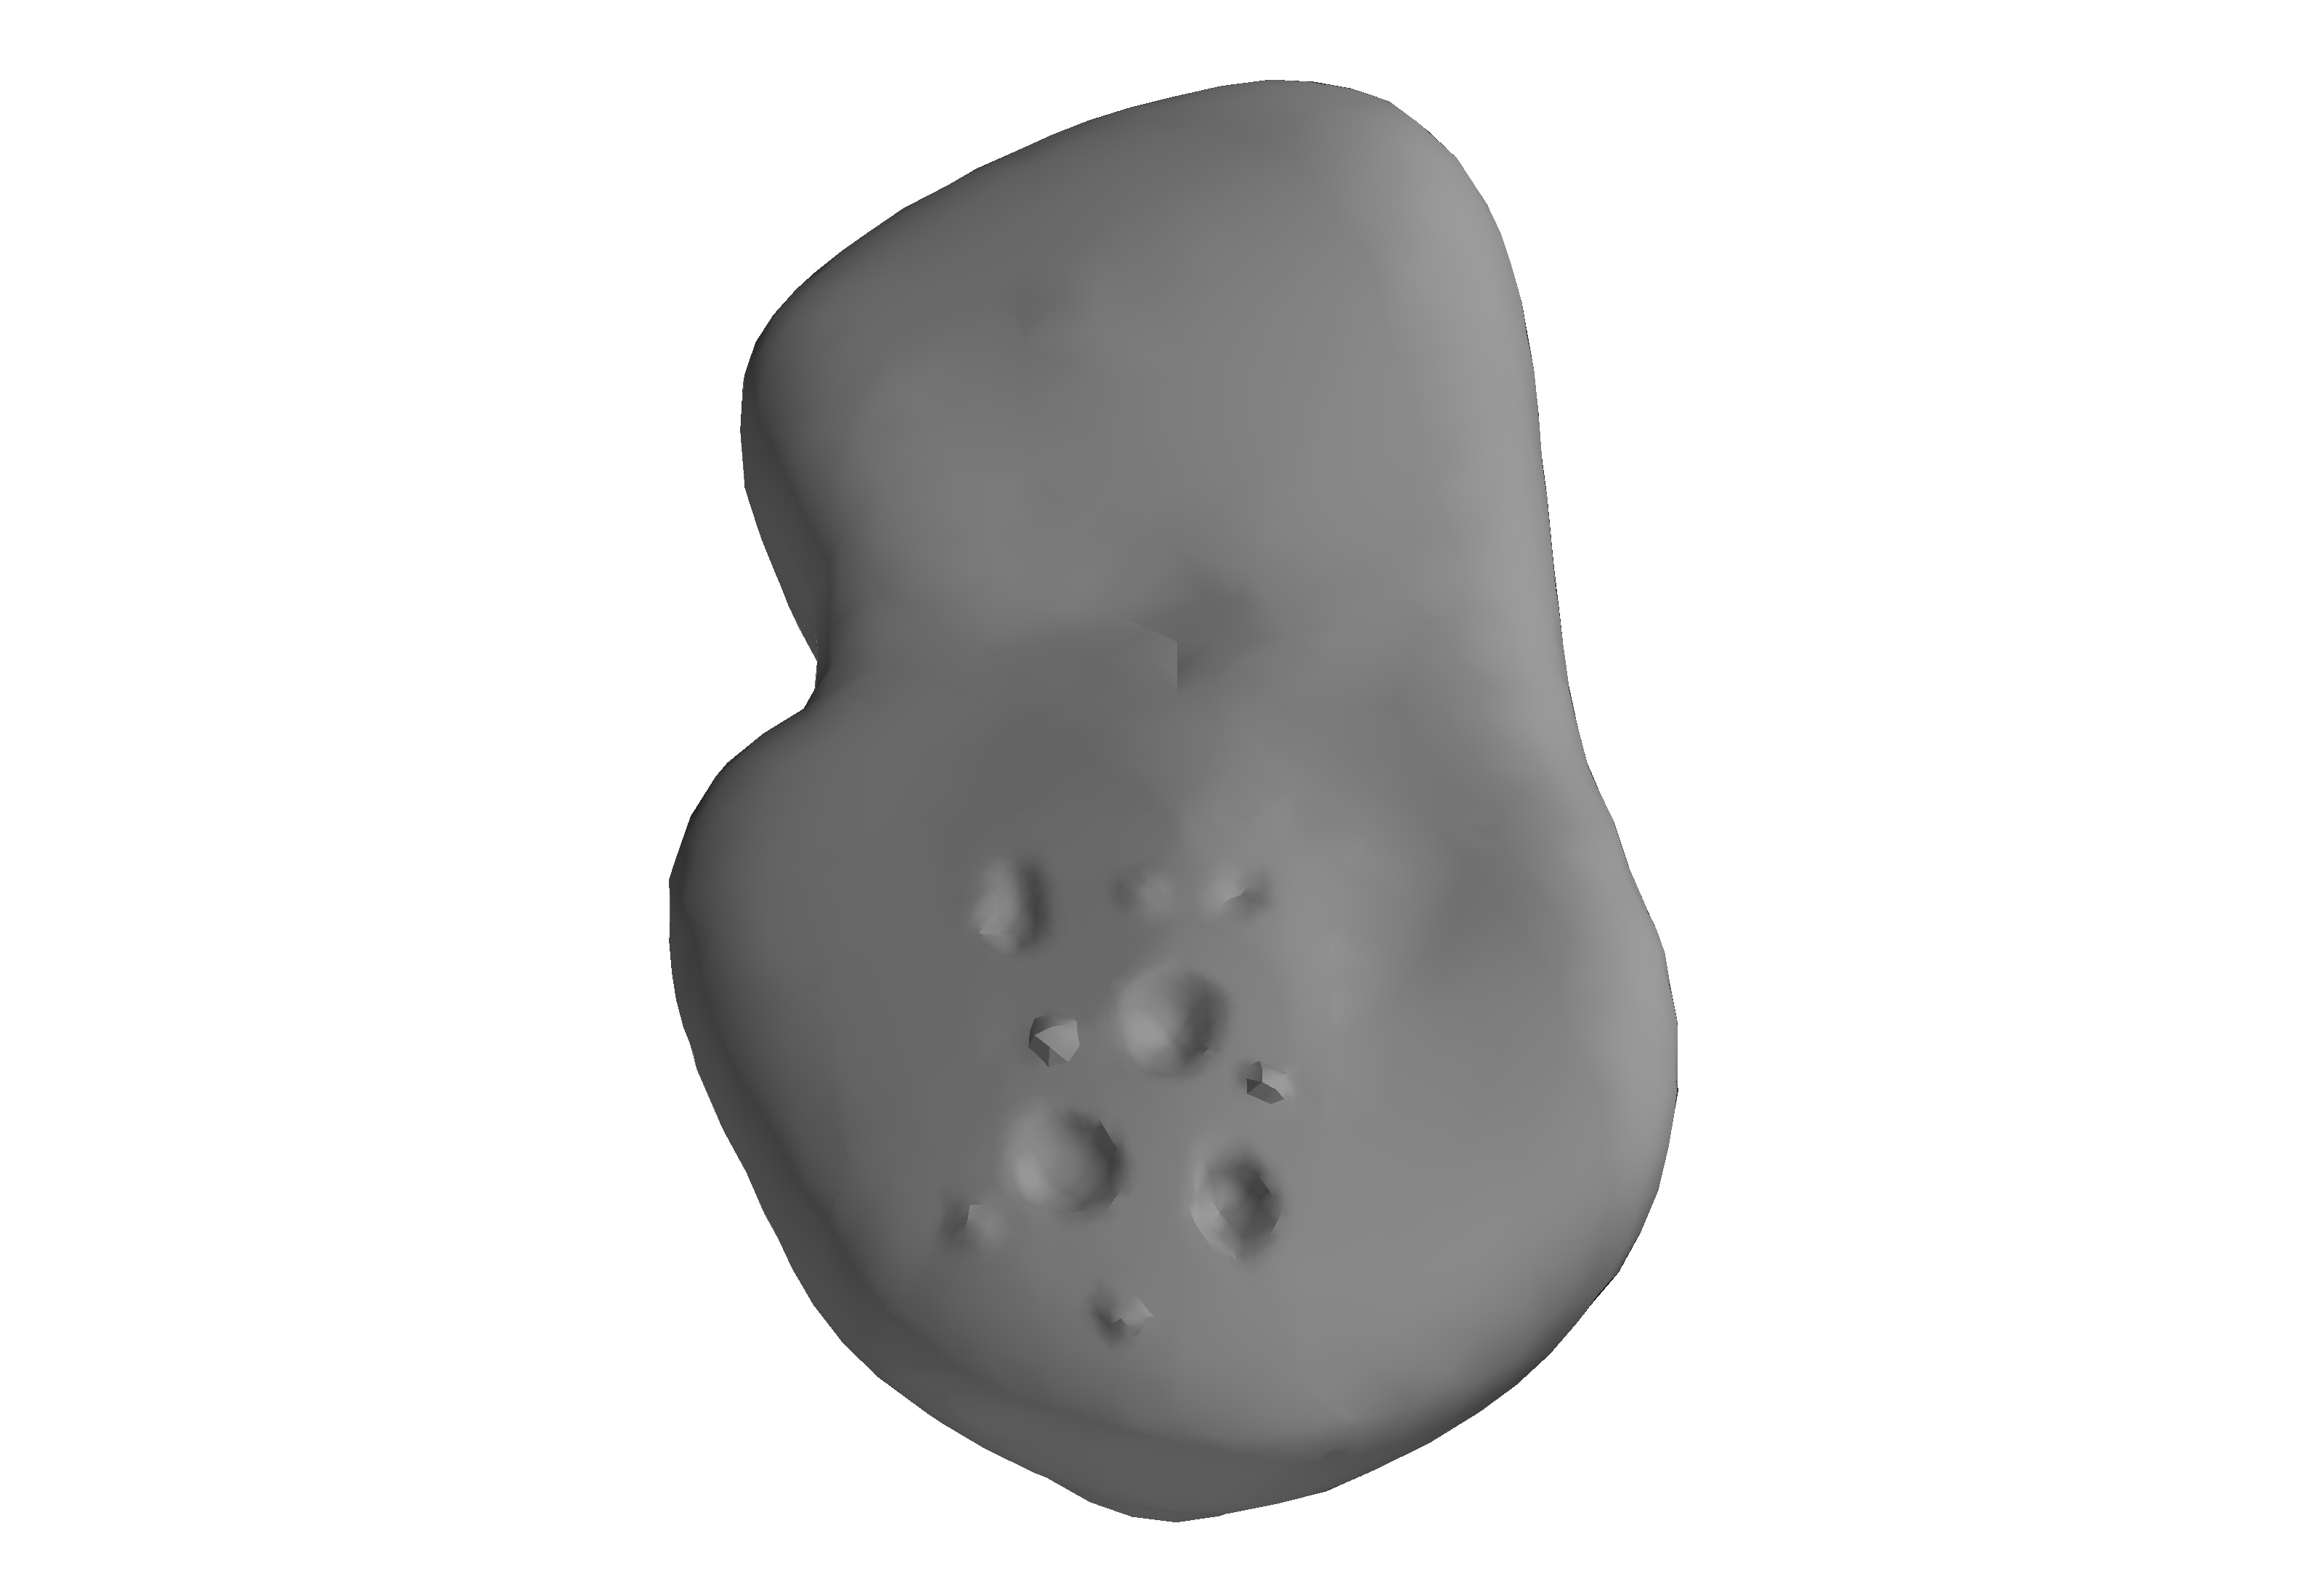
\includegraphics[width=0.5\textwidth]{figures/computational_geometry/dynamic_exploration/castalia_bump_true.jpg}}~
    \subcaptionbox{Estimated shape model after measuring the surface\label{fig:bump_castalia}}{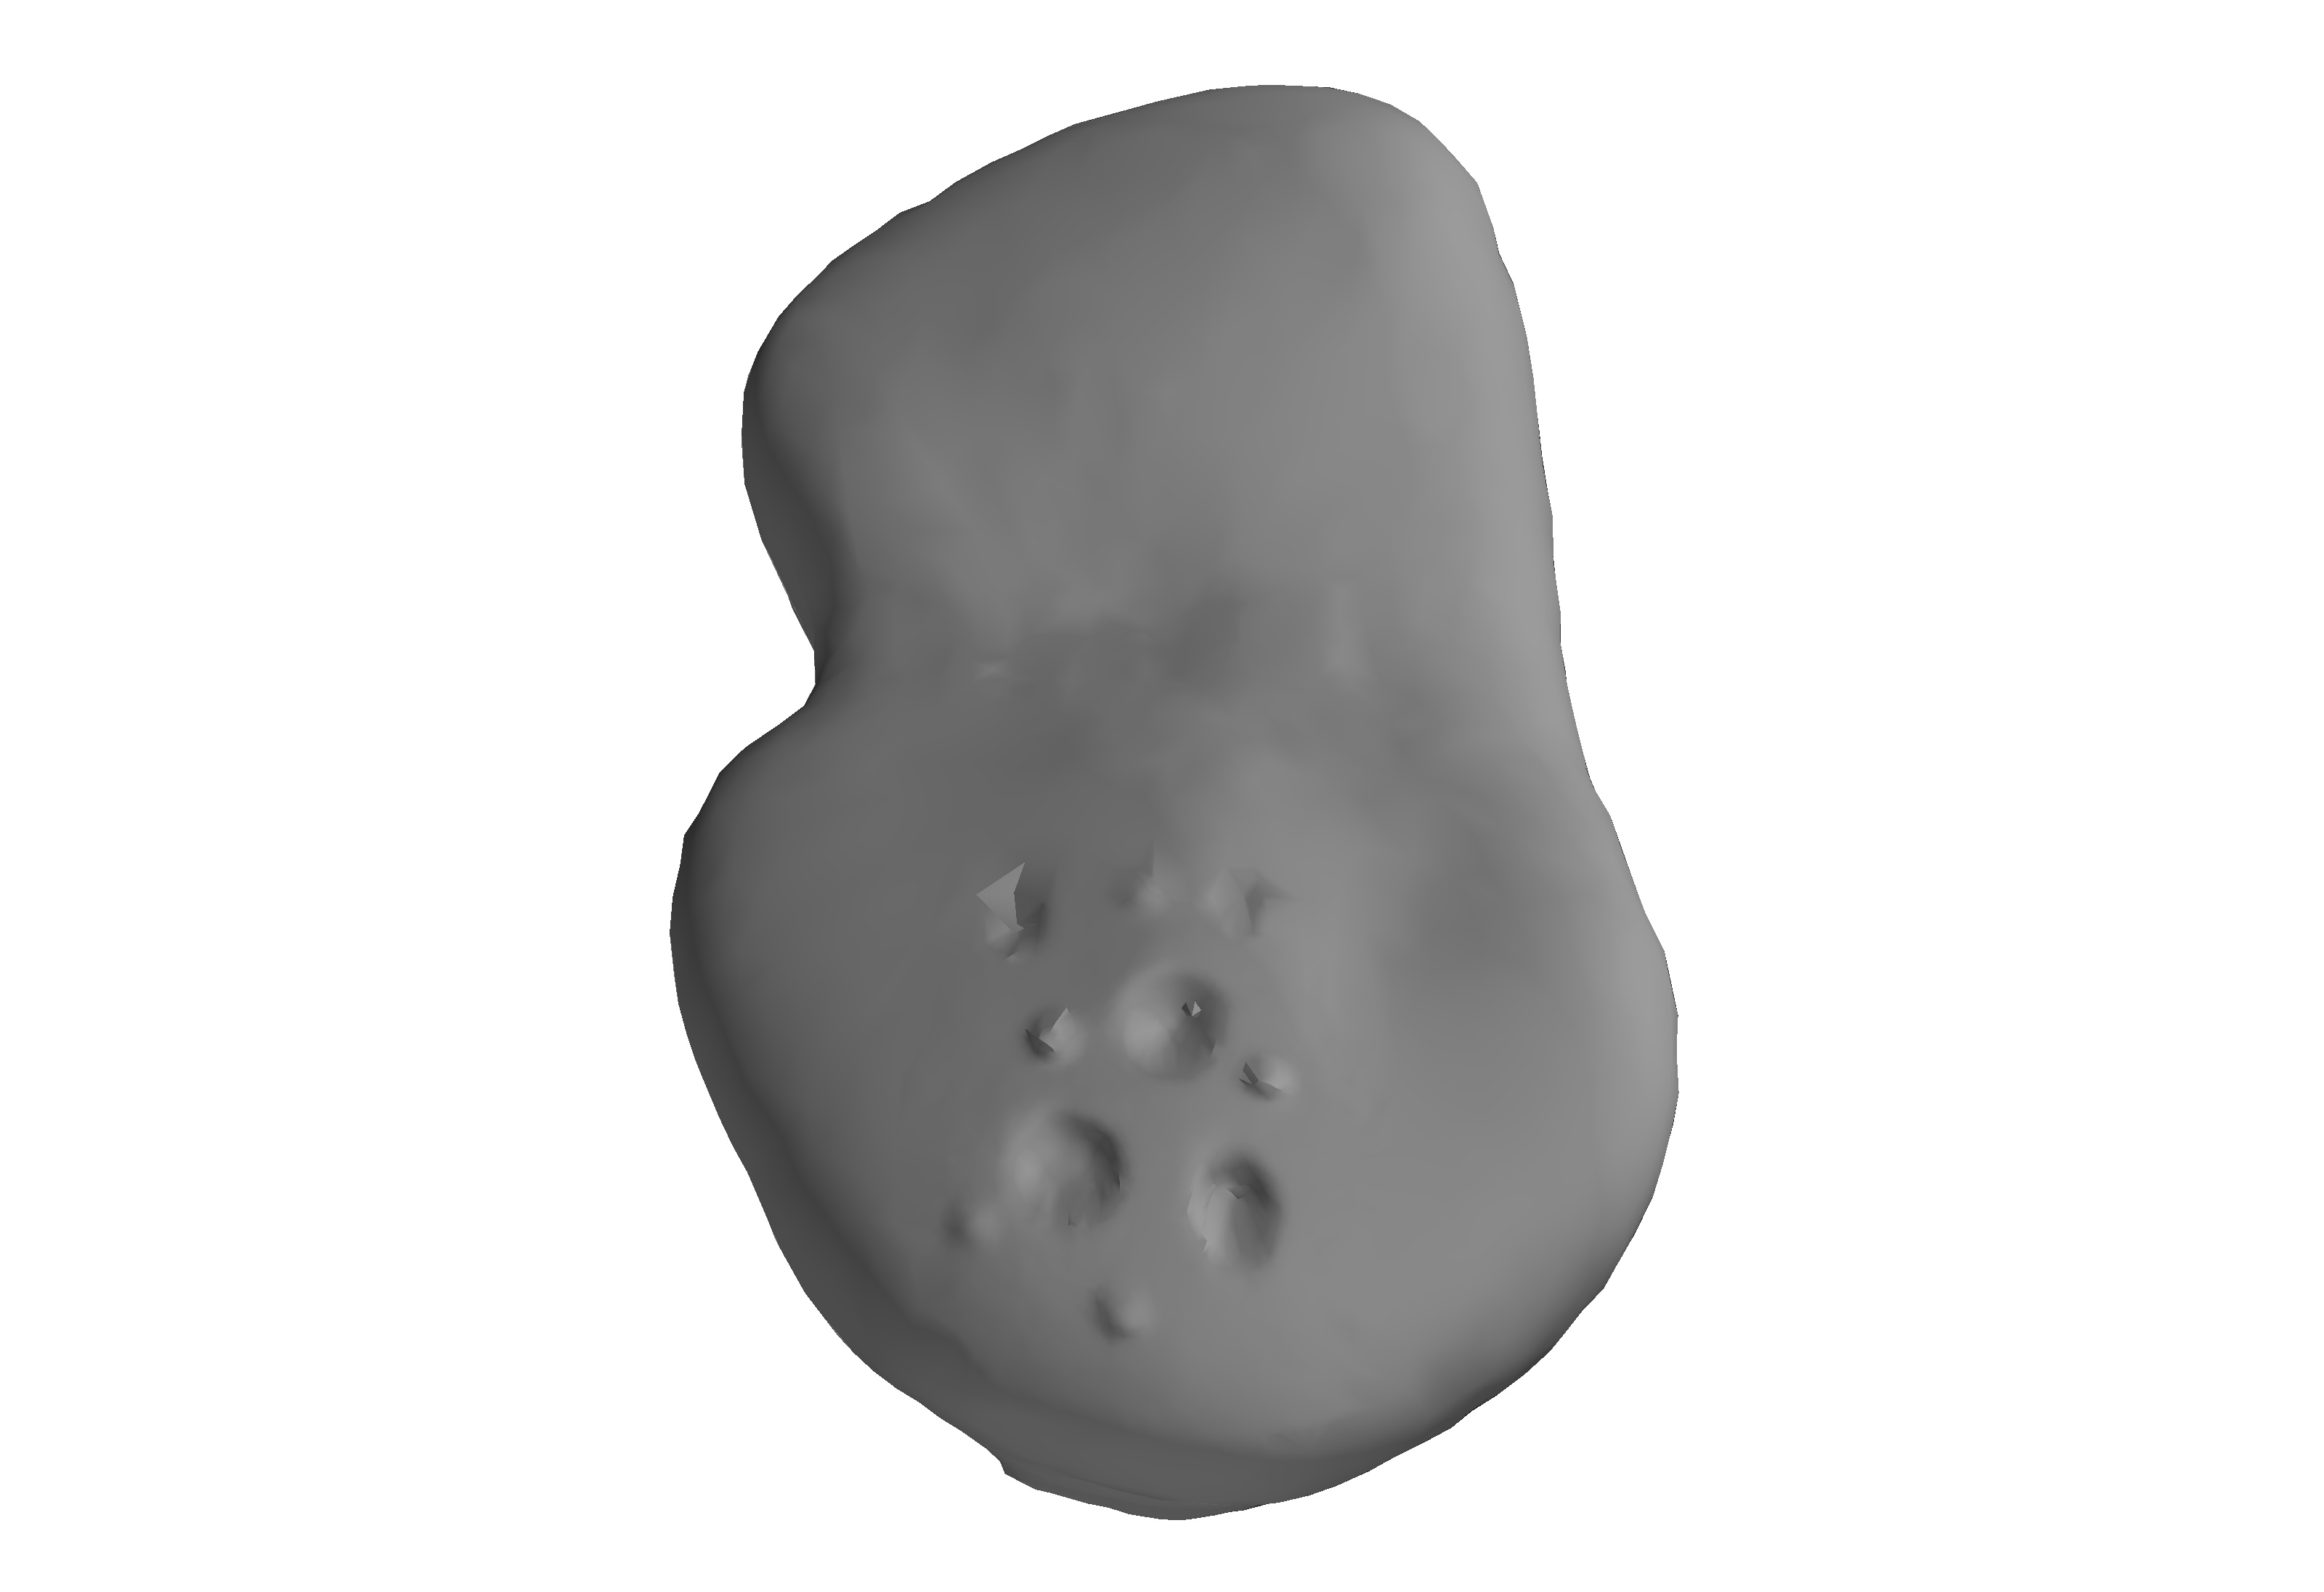
\includegraphics[width=0.5\textwidth]{figures/computational_geometry/dynamic_exploration/castalia_bump_est.jpg}}
    \caption{Estimated reconstruction of augmented Castalia with landing features~\label{fig:bumpy_castalia}}
\end{figure}

\section{Shape Reconstruction Examples}
In this section, we demonstrate the use of the results presented in~\cref{sec:dumbbell_model,sec:se3_control,sec:shape_reconstruction} with several numerical examples.
The incremental mesh update approach from~\cref{sec:radius_update} is used to iteratively reconstruct the shape of several asteroid given \gls{lidar} measurements.
We utilize radar shape models of asteroids \num{4769} Castalia, (\num{52760}) \num{1998} \(\text{ML}_{14}\), \num{1620} Geographos, and 6489 Golevka~\cite{neese2004}.
The asteroids exhibit a wide range of shapes and demonstrate the effectiveness of the mesh update approach.
\Cref{sec:kinematic_exploration} focuses on the application of the incremental mesh update scheme of~\cref{sec:radius_update} for several different asteroids.
\Cref{sec:dynamic_exploration} incorporates the full dynamic model on \( \SE \) of a dumbbell spacecraft given in~\cref{sec:inertial_dumbbell_eoms}, the polyhedron potential model from~\cref{sec:polyhedron_potential}, and the mesh update and guidance scheme presented in~\cref{sec:radius_update}.

\subsection{Kinematic Model}\label{sec:kinematic_exploration}
The results utilize a kinematics only model of the spacecraft and dynamics instead of the full dynamic simulation. 
We ignore the dynamics of the asteroid and spacecraft and instead focus soley on the shape reconstruction.
\Cref{tab:kinematic_asteroids} lists the true shape model parameters of asteroids Geographos and Golevka.
\begin{table}[htbp]
    \centering
    \begin{tabular}{lccc}
        \toprule
        Asteroid & Semi-major axes (\si{\kilo\meter}) & Vertices & Faces\\
        \midrule
        \num{1620} Geographos & \( 2.5 \times 1.0 \times 1.05 \) & \num{8192} & \num{16380}  \\
        \num{6489} Golevka & \( 0.53 \times 0.53 \times 0.53 \)  & \num{2048} & \num{4092} \\
        \bottomrule
    \end{tabular} 
    \caption{Asteroid properties for kinematic only exploration~\label{tab:kinematic_asteroids}}
\end{table}
The spacecraft is assumed to be able to arbitrarily move around the asteroid and collect measurements.
The simulations begin with an triaxial ellipsoid mesh that is sized to match the semi-major axes of each asteroid.
With this estimate, measurements are made of the surface and used to reconstruct the true shape following the process in~\cref{sec:radius_update}.
\Gls{lidar} measurements are generated until the total uncertainty
\begin{align*}
    \sum_i w_i,
\end{align*}
is sufficiently small.
In addition, we compute the volume of the estimate shape throughout the simulation using the algorithm presented in~\cref{proof:polyhedron_volume}.

\begin{figure}[htbp]
    \centering
    \subcaptionbox{Initial Shape Estimate\label{fig:geographos_partial_0}}{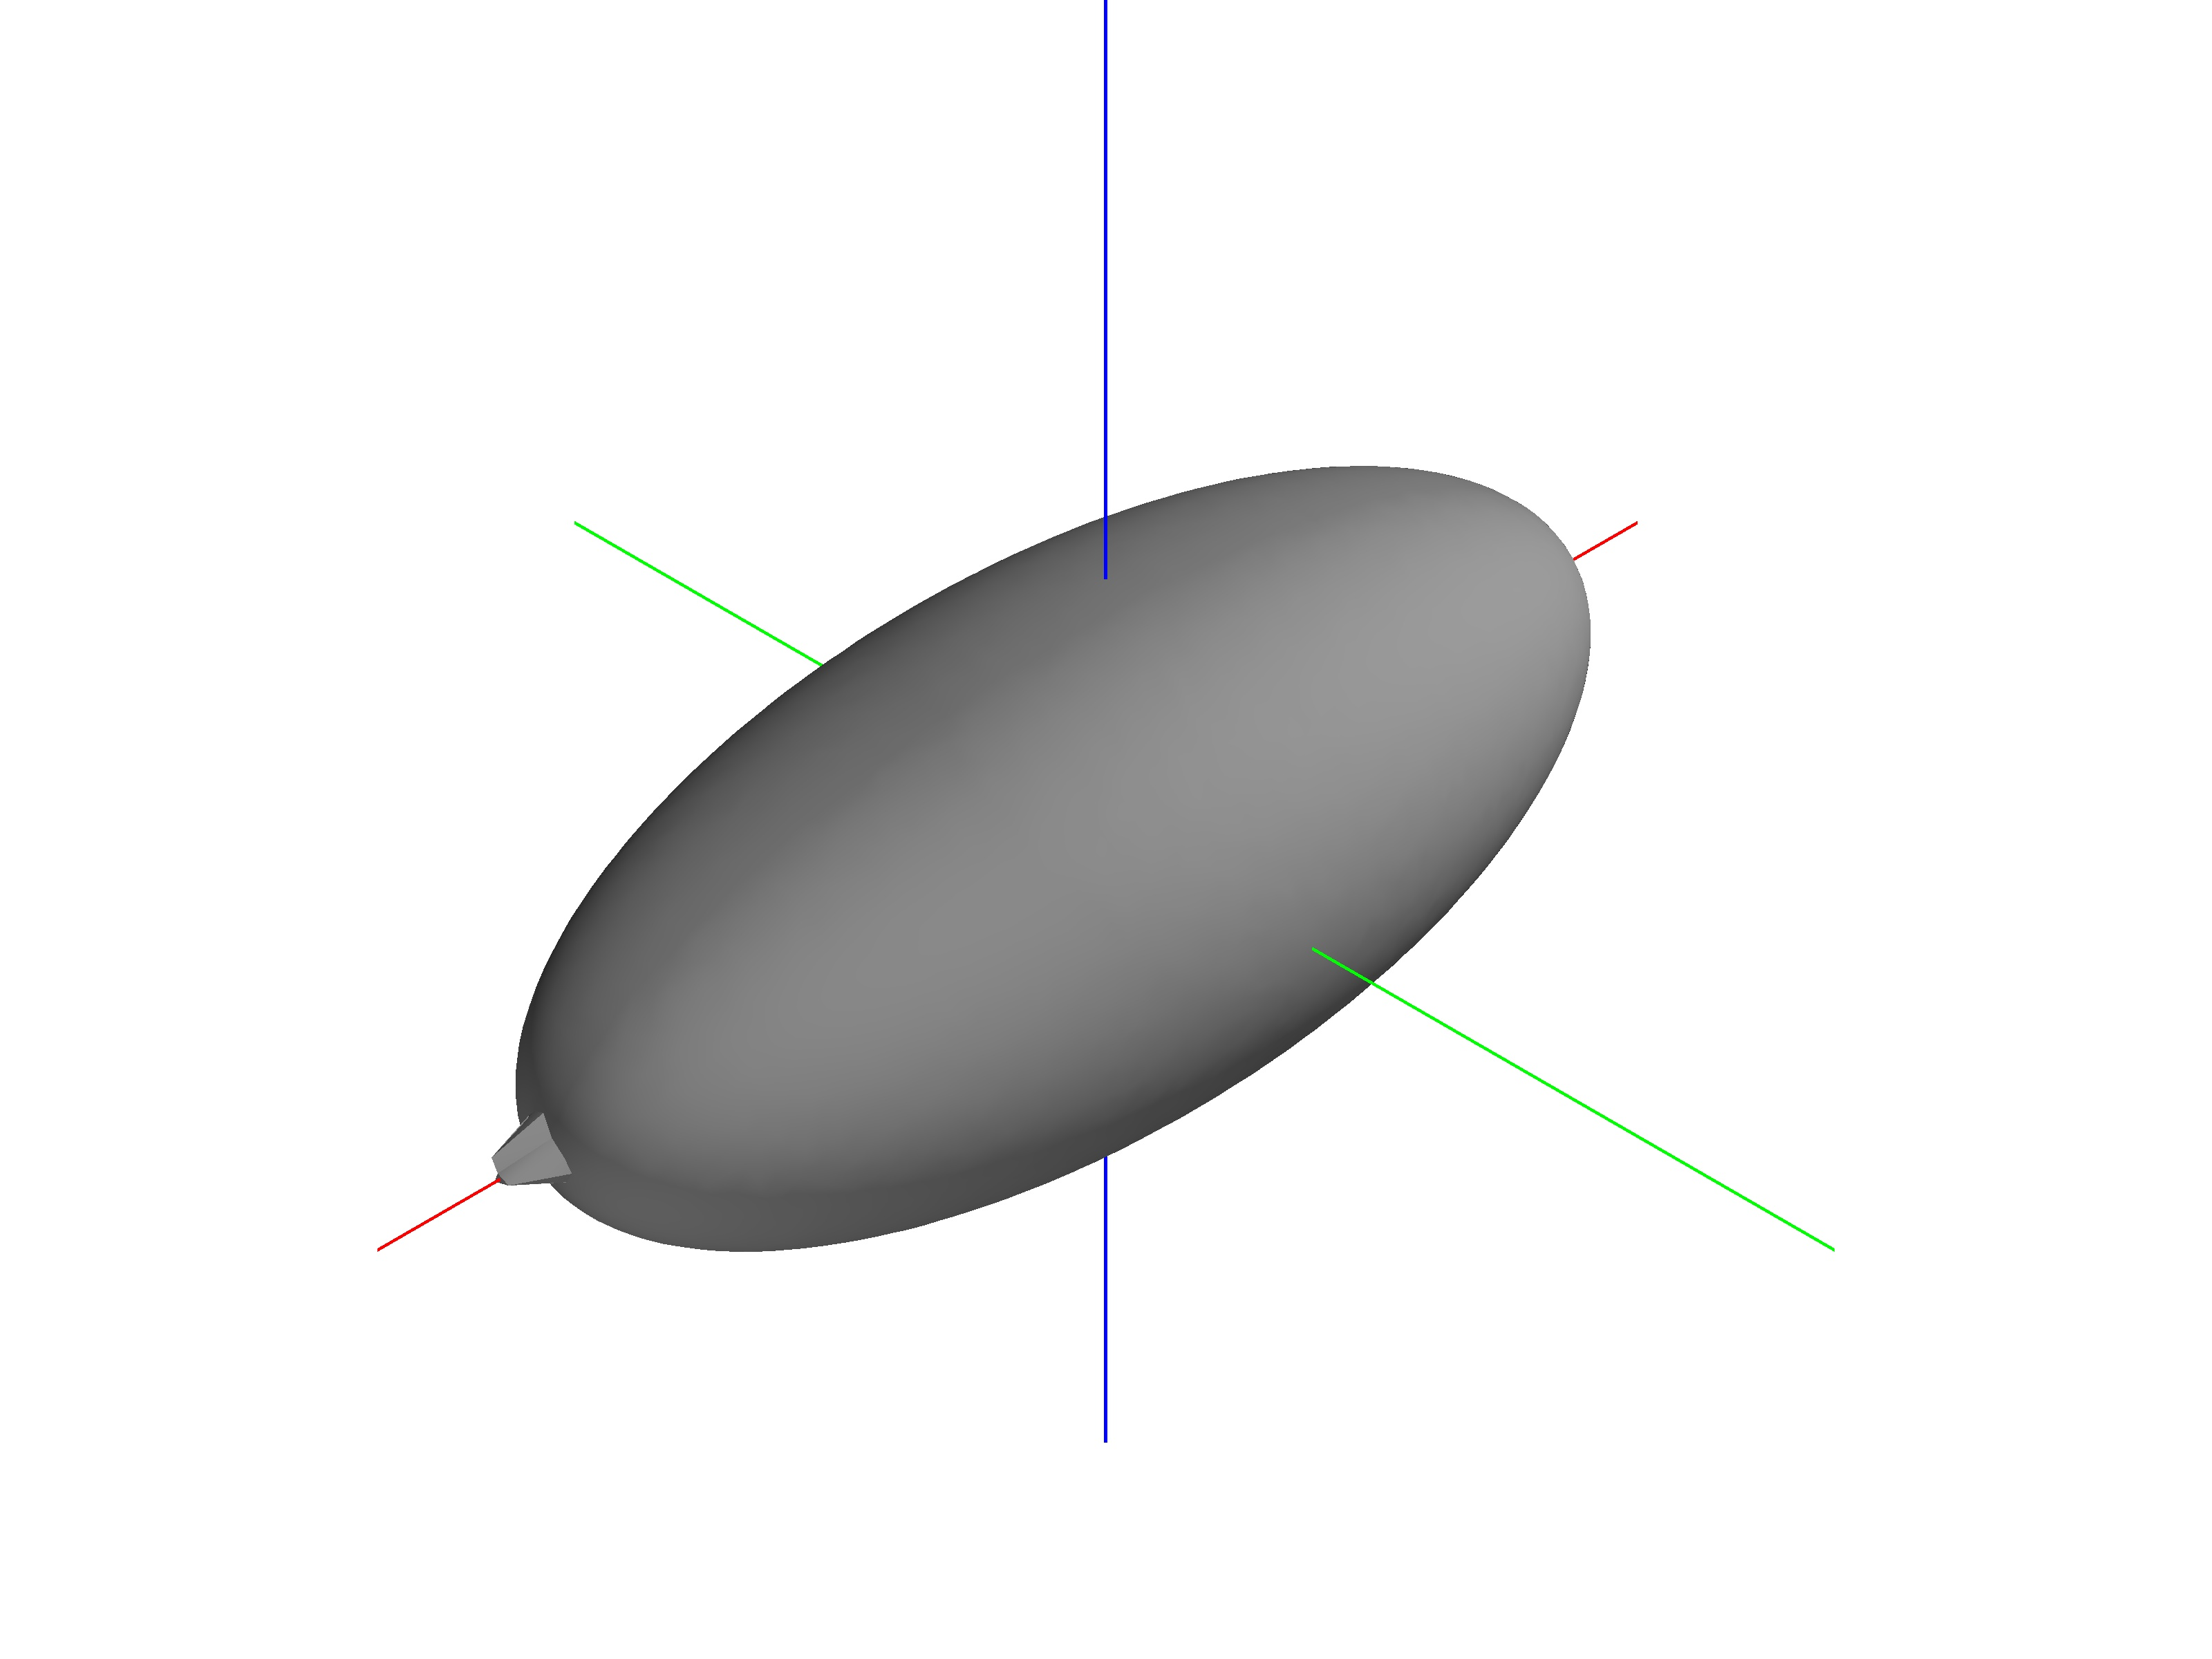
\includegraphics[height=0.5\textheight,width=0.5\textwidth,keepaspectratio]{figures/computational_geometry/mesh_update/geographos/partial_0.jpg}}~
    \subcaptionbox{\SI{25}{\percent} of measurements added\label{fig:geographos_partial_25}}{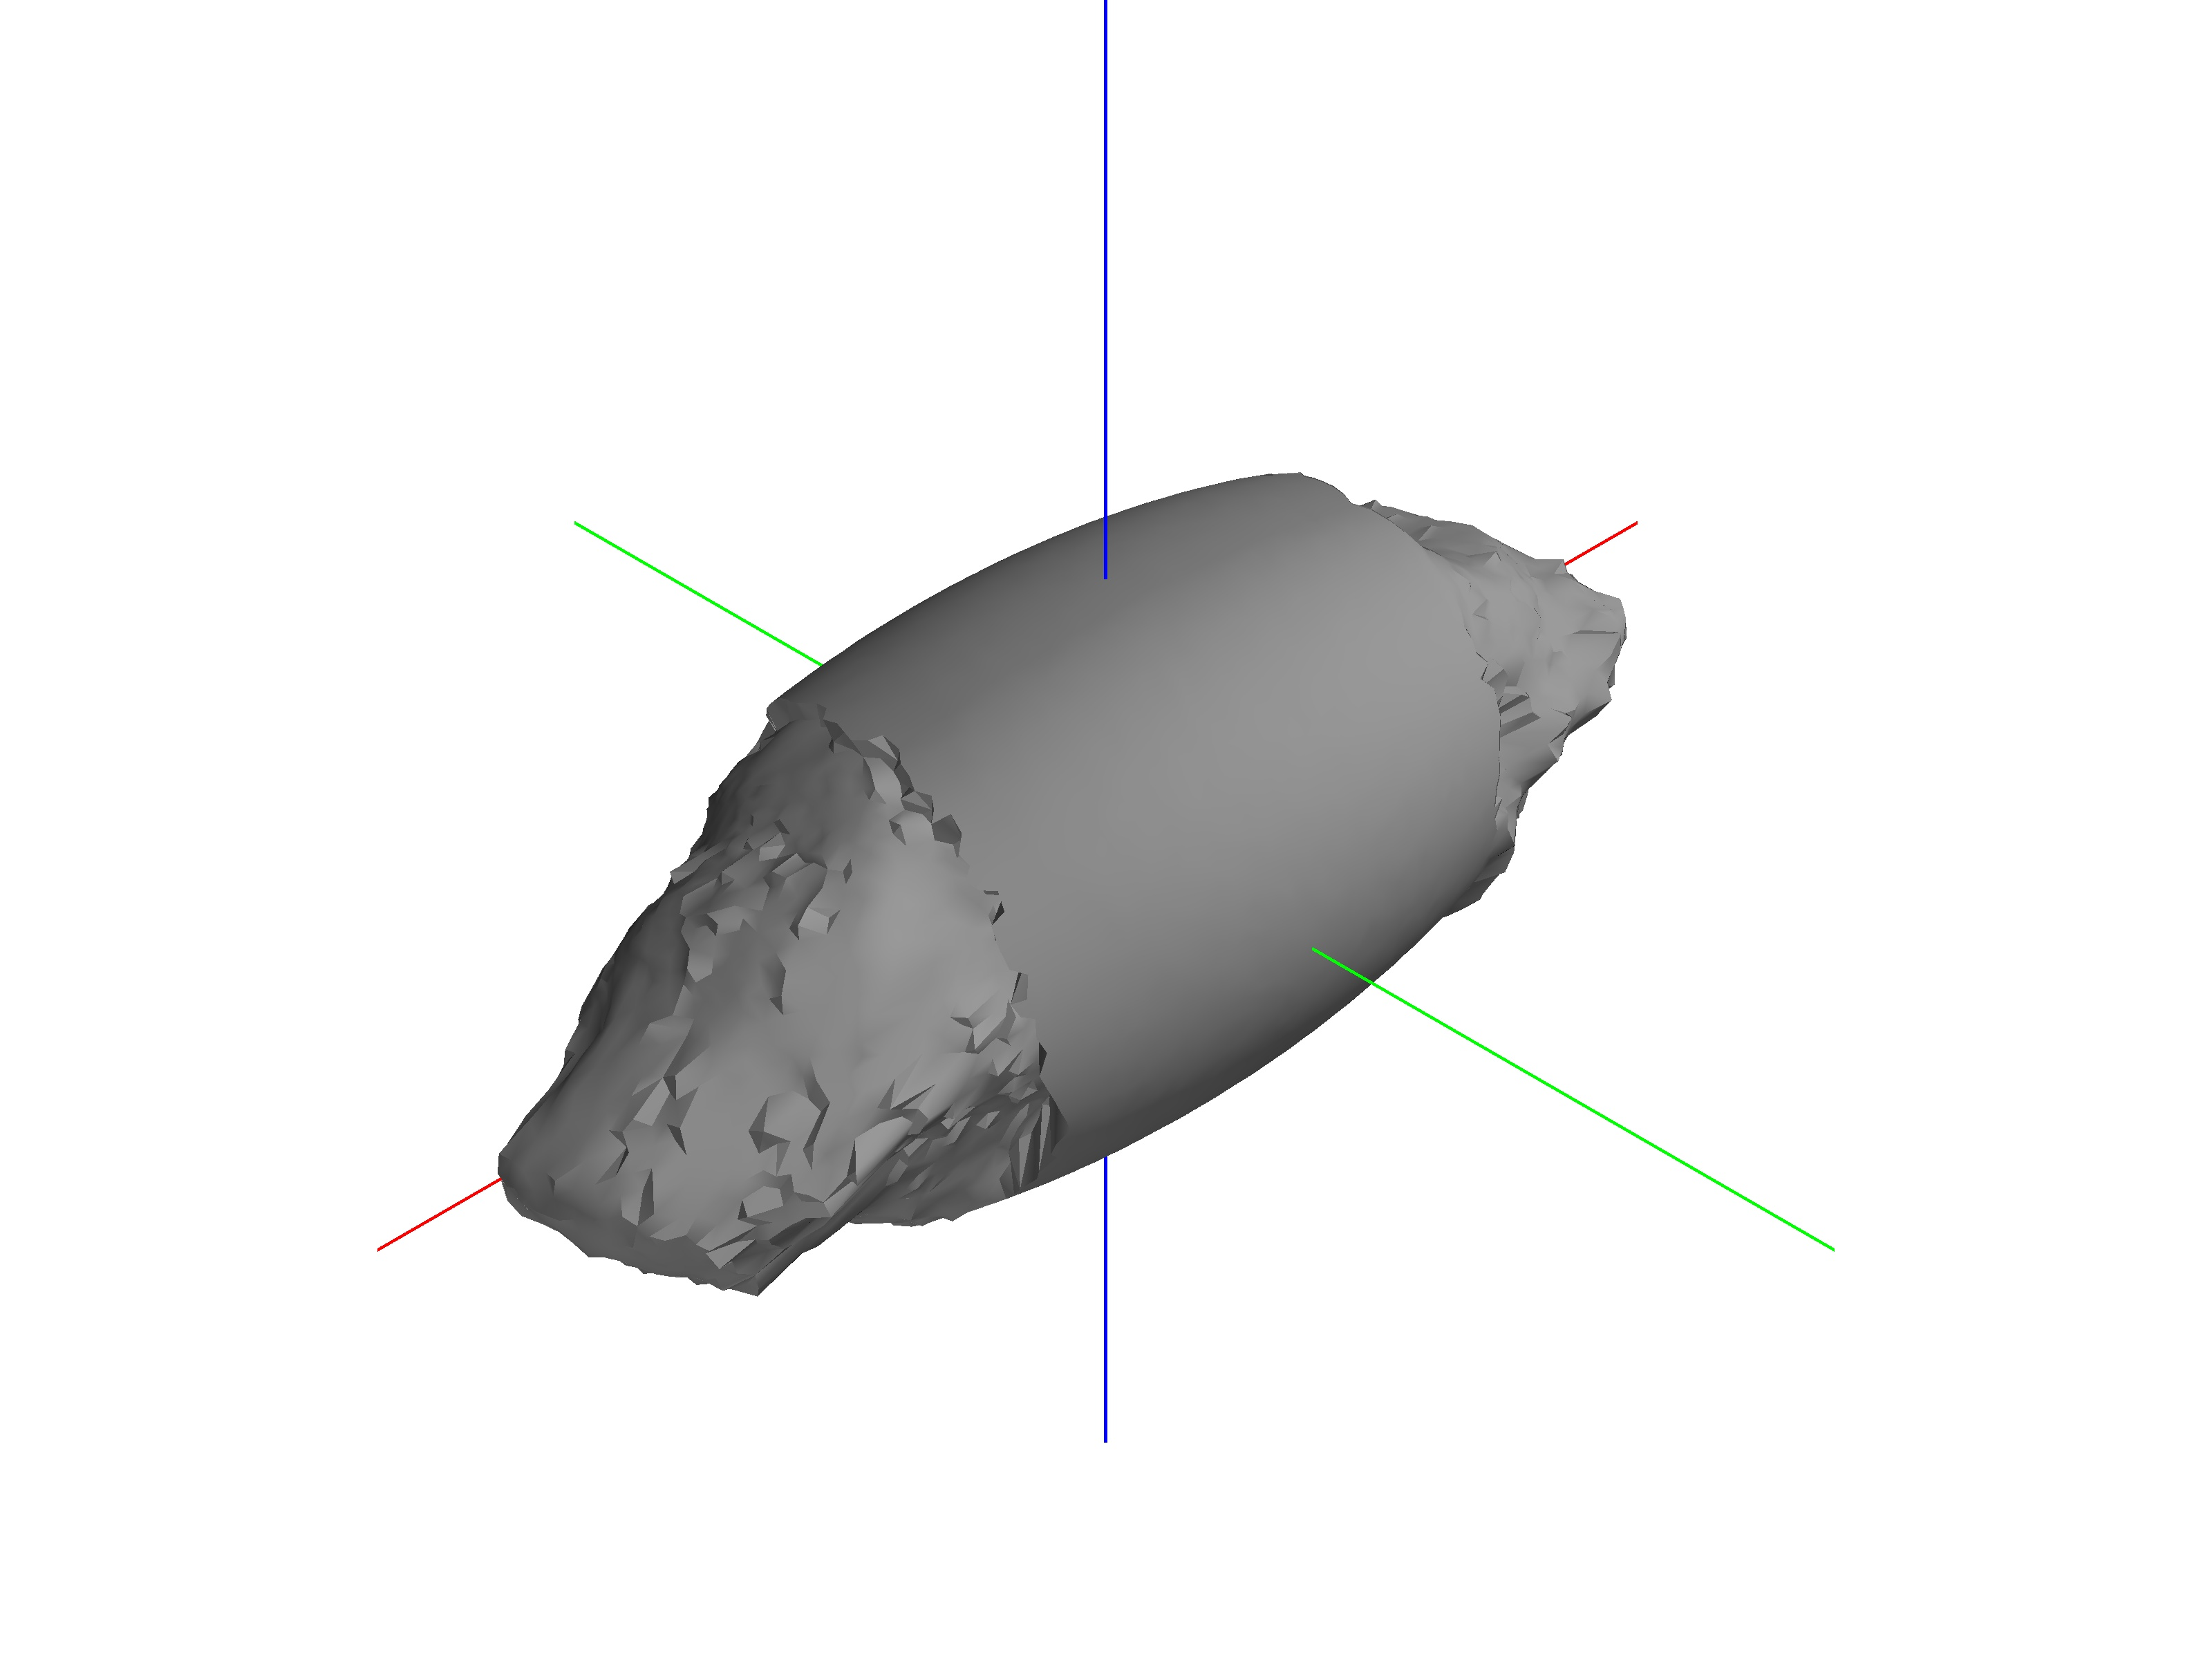
\includegraphics[width=0.5\textwidth]{figures/computational_geometry/mesh_update/geographos/partial_1872.jpg}}

    \subcaptionbox{\SI{50}{\percent} of measurments added\label{fig:geographos_partial_50}}{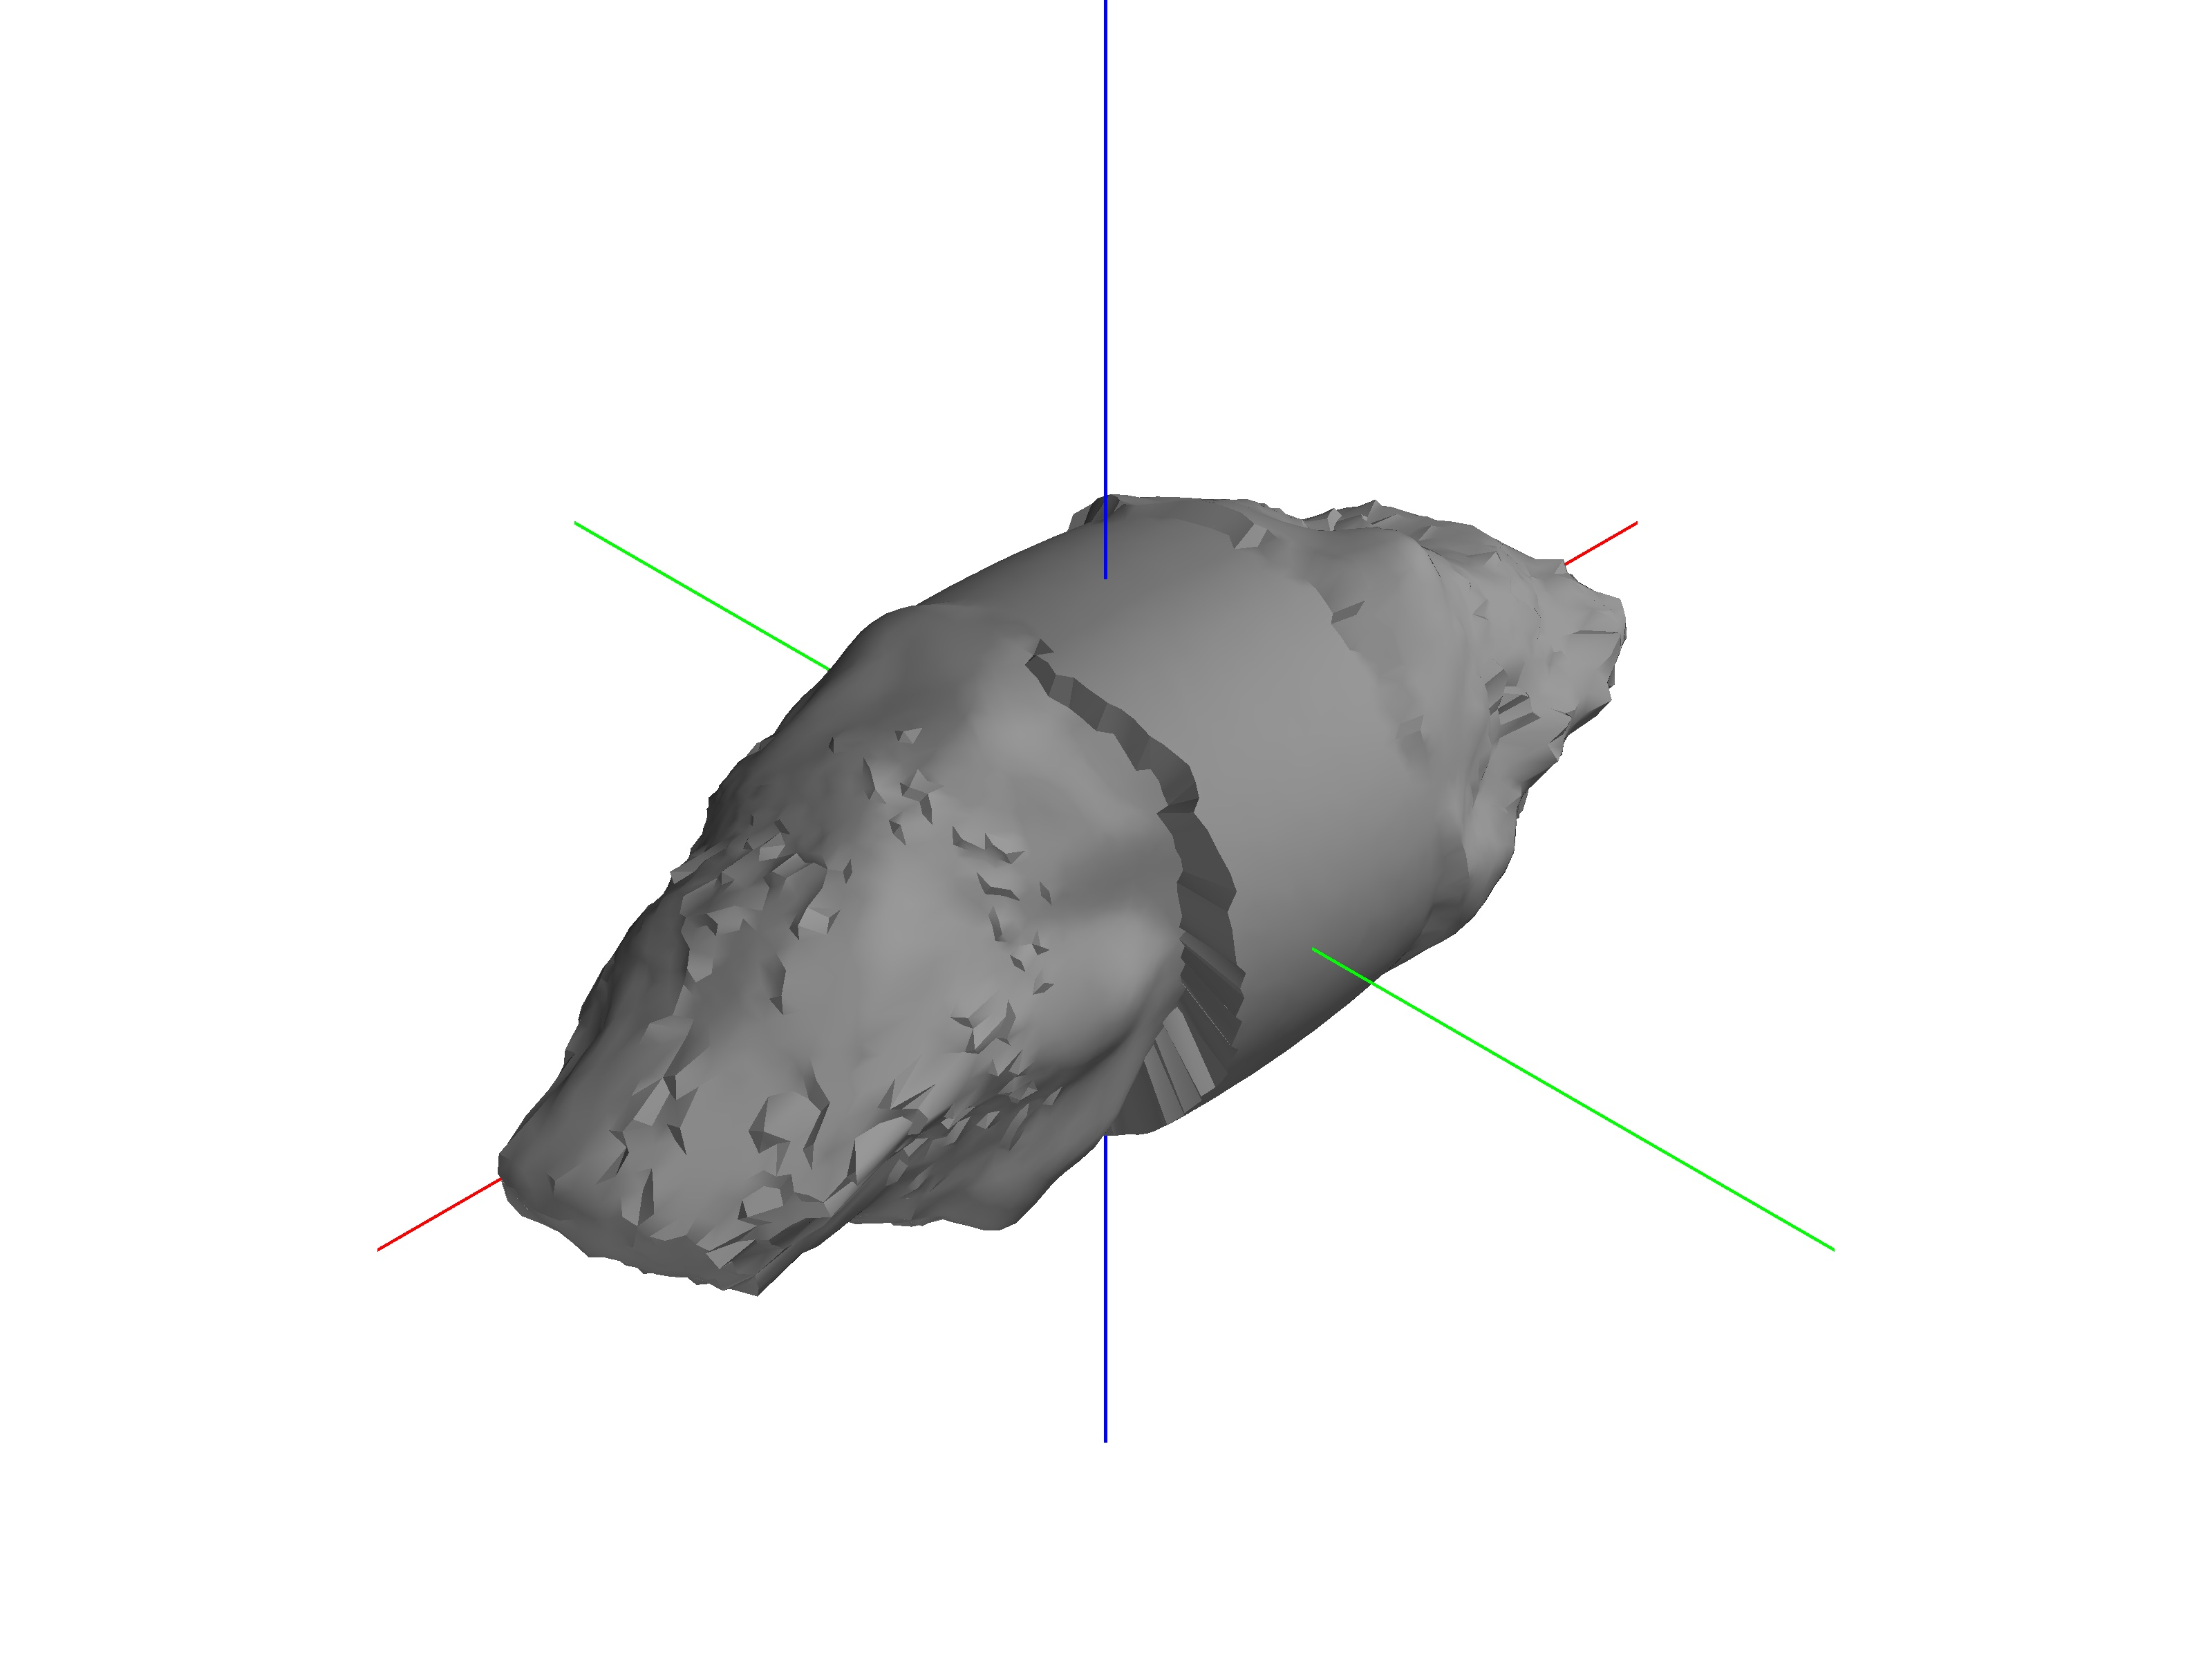
\includegraphics[width=0.5\textwidth]{figures/computational_geometry/mesh_update/geographos/partial_3745.jpg}}~
    \subcaptionbox{\SI{75}{\percent} of measurements added\label{fig:geographos_partial_75}}{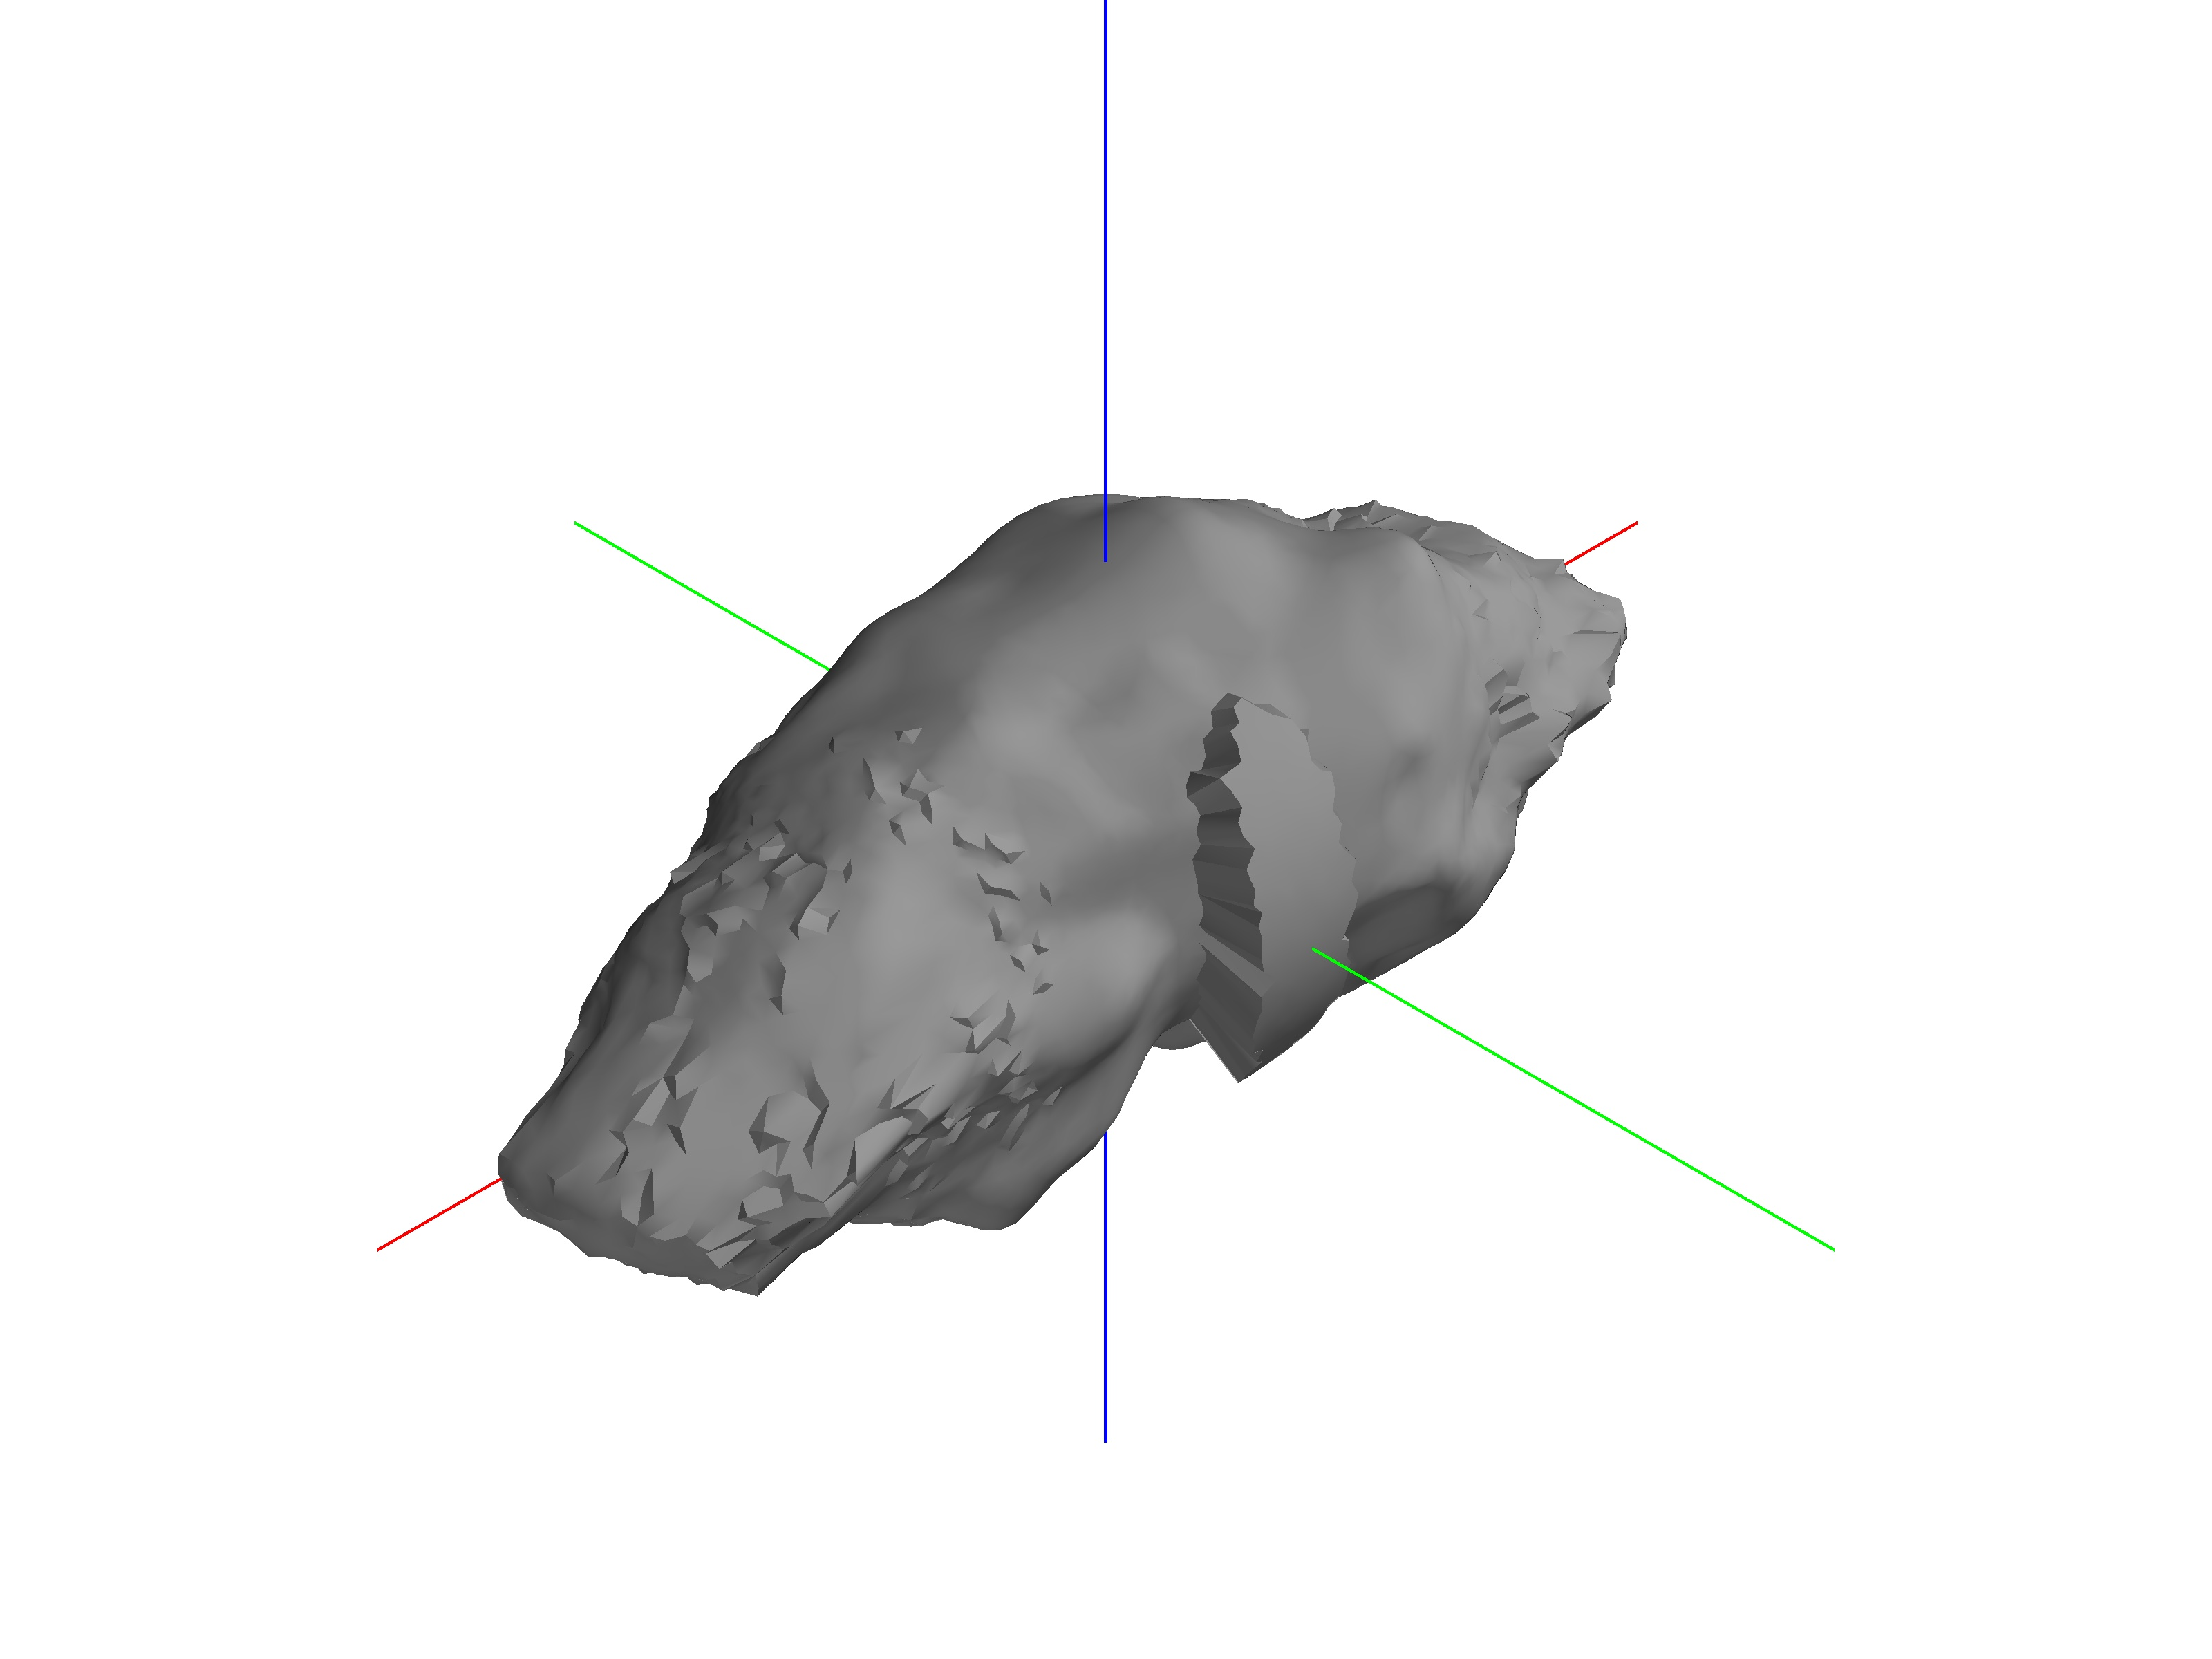
\includegraphics[width=0.5\textwidth]{figures/computational_geometry/mesh_update/geographos/partial_5617.jpg}}

    \subcaptionbox{\SI{100}{\percent} of measurements added\label{fig:geographos_partial_100}}{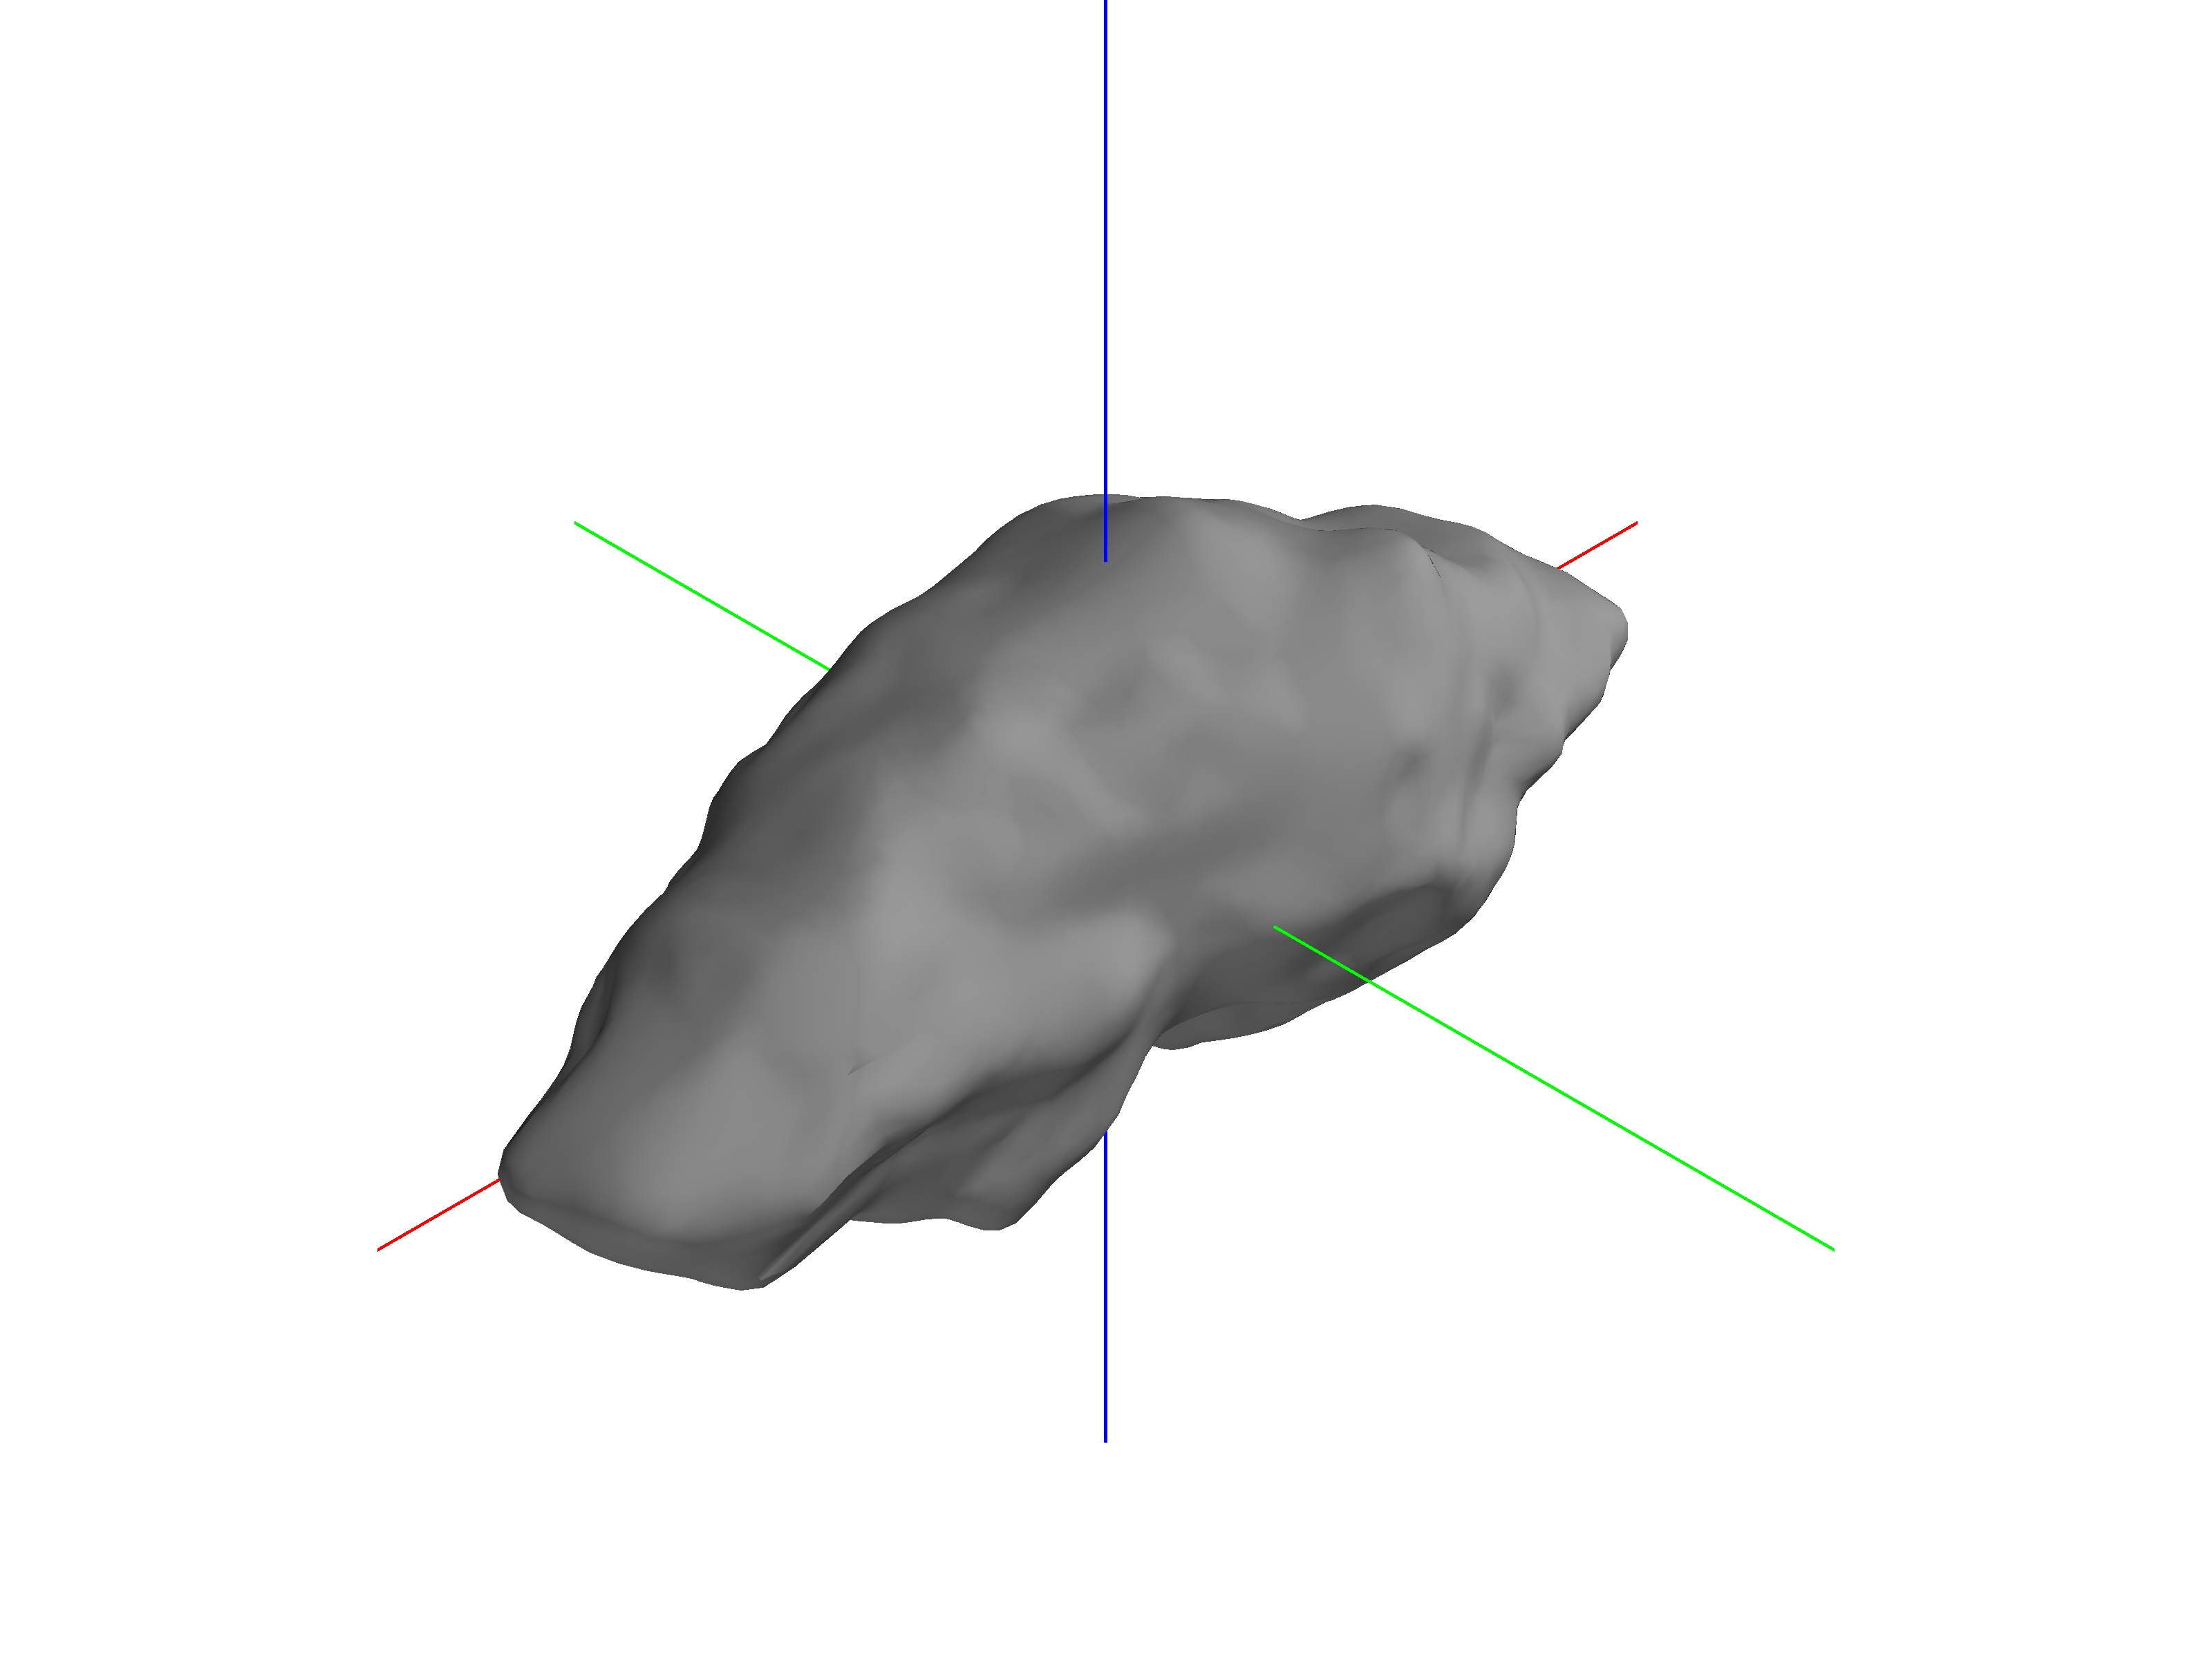
\includegraphics[width=0.5\textwidth]{figures/computational_geometry/mesh_update/geographos/partial_7489.jpg}}~
    \subcaptionbox{True Shape Model\label{fig:geographos_truth}}{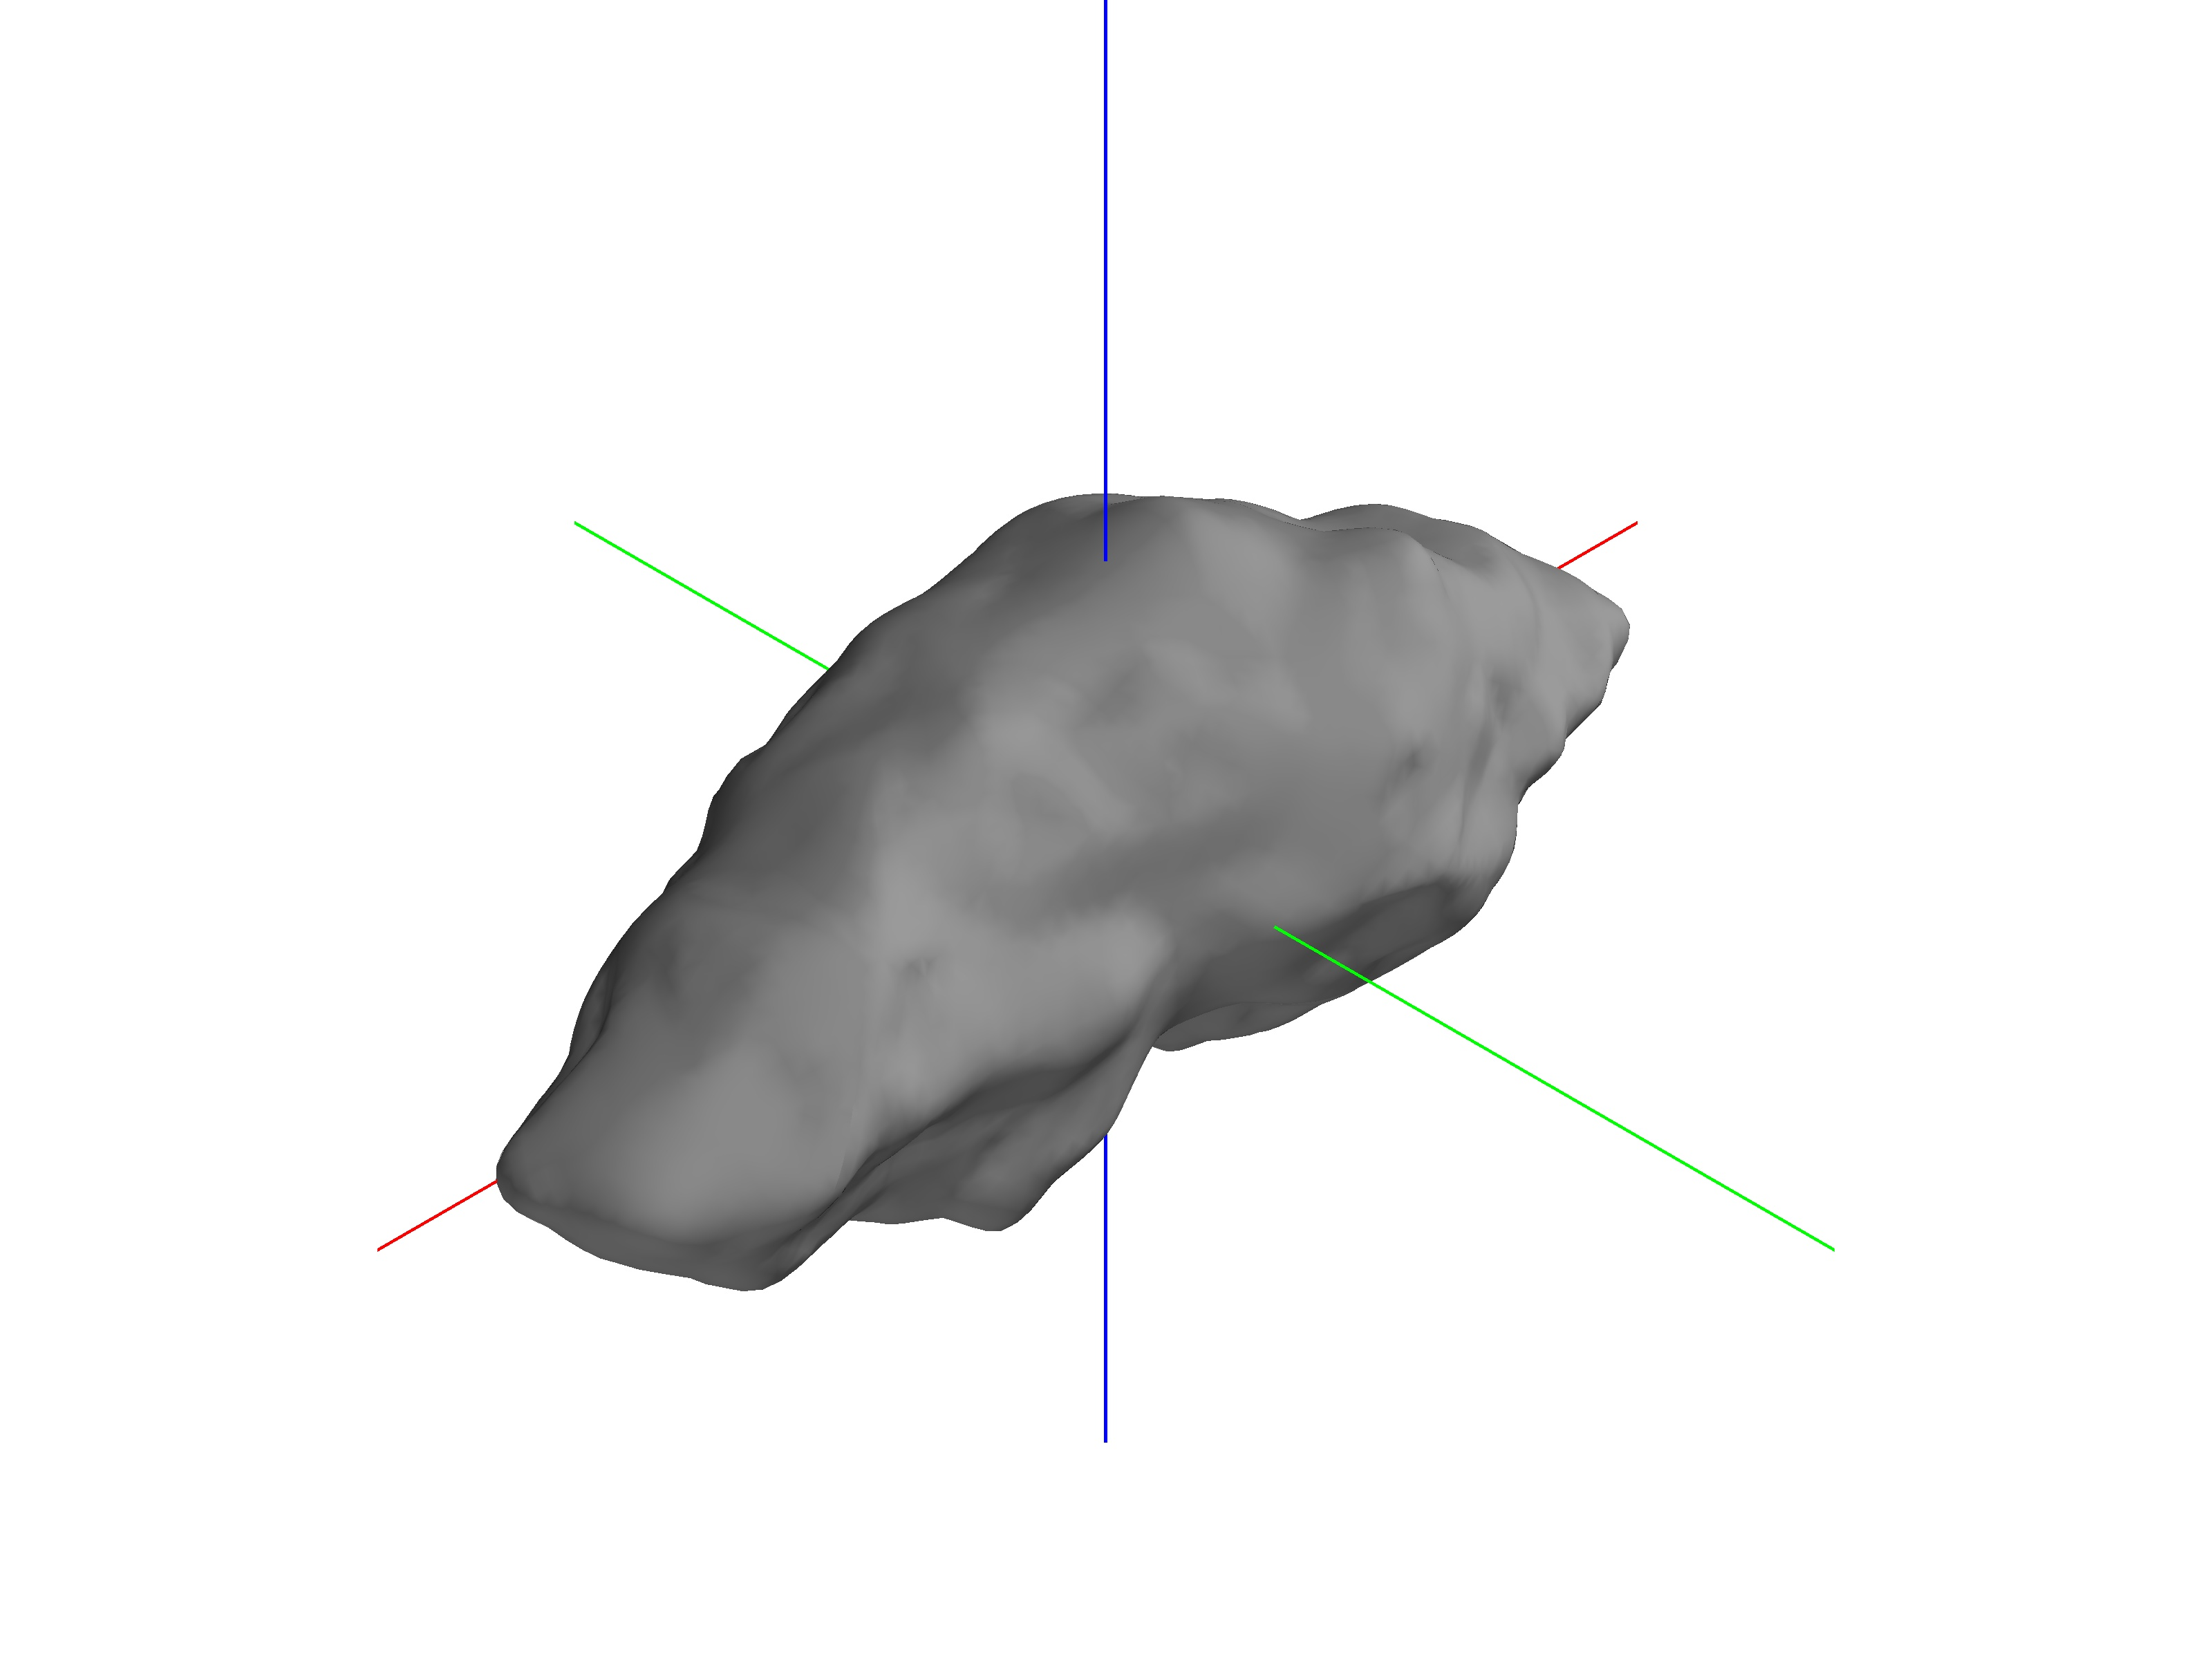
\includegraphics[width=0.5\textwidth]{figures/computational_geometry/mesh_update/geographos/truth.jpg}}
    \caption[Asteroid Geographos Incremental Reconstruction]{Incremental Reconstruction of asteroid Geographos~\label{fig:geographos_reconstruction}}
\end{figure}
\num{1620} Geographos is a highly elongated stony asteroid of the Apollo group.
Discoved in \num{1951}, Geographos is a potentially hazardous asteroid which passes sufficiently close to the Earth to present a hazard.
\Cref{fig:geographos_reconstruction} shows the shape reconstruction for asteroid Geographos at several distinct points during the process.
Comparing~\cref{fig:geographos_partial_100,fig:geographos_truth} shows that the final shape closely matches the true radar model.
In~\cref{fig:geographos_metrics} we display the vertex uncertainty and mesh volume as a function of time.
\begin{figure}[htbp]
    \centering
    \subcaptionbox{Normalized Uncertainty\label{fig:geographos_uncertainty}}{\includegraphics[width=0.5\textwidth,height=0.31\textwidth]{tikz/geographos_uncertainty.tikz}}~
    \subcaptionbox{Volume Percent Error\label{fig:geographos_volume}}{\includegraphics[width=0.5\textwidth,height=0.31\textwidth]{tikz/geographos_volume.tikz}}
    \caption{Normalized uncertainty and volume percent error for Geographos\label{fig:geographos_metrics}}
\end{figure}
The plots show the the reconstruction achieves an accurate shape estimate with a total volume which closesly matches the true volume.

\num{6489} Golevka is a small angular shaped asteroid of the Apollo group.
Discoved in \num{1995}, Golevka is a potentially hazardous asteroid which passes sufficiently close to the Earth to present a hazard.
\Cref{fig:golevka_reconstruction} shows the shape reconstruction for asteroid Geographos at several distinct points during the process.
Comparing~\cref{fig:golevka_partial_100,fig:golevka_truth} shows that the final shape closely matches the true radar model.
In~\cref{fig:golevka_metrics} we display the vertex uncertainty and mesh volume as a function of time.
\begin{figure}[htbp]
    \centering
    \subcaptionbox{Normalized Uncertainty\label{fig:golevka_uncertainty}}{\includegraphics[width=0.5\textwidth,height=0.31\textwidth]{tikz/golevka_uncertainty.tikz}}~
    \subcaptionbox{Volume Percent Error\label{fig:golevka_volume}}{\includegraphics[width=0.5\textwidth,height=0.31\textwidth]{tikz/golevka_volume.tikz}}
    \caption{Normalized uncertainty and volume percent error for Golevka\label{fig:golevka_metrics}}
\end{figure}
The plots show the the reconstruction achieves an accurate shape estimate with a total volume which closesly matches the true volume.
It is interesting to note that the reconstruction of Golevka achieves an accurate shape reconstruction in a much smaller amount of time as compared to Geographos.
This is primarily due to the smaller size of Golevka and the relatively spherical shape of the body in contrast to the highly elliptical shape of Geographos.
\begin{figure}[htbp]
    \centering
    \subcaptionbox{Initial Shape Estimate\label{fig:golevka_partial_0}}{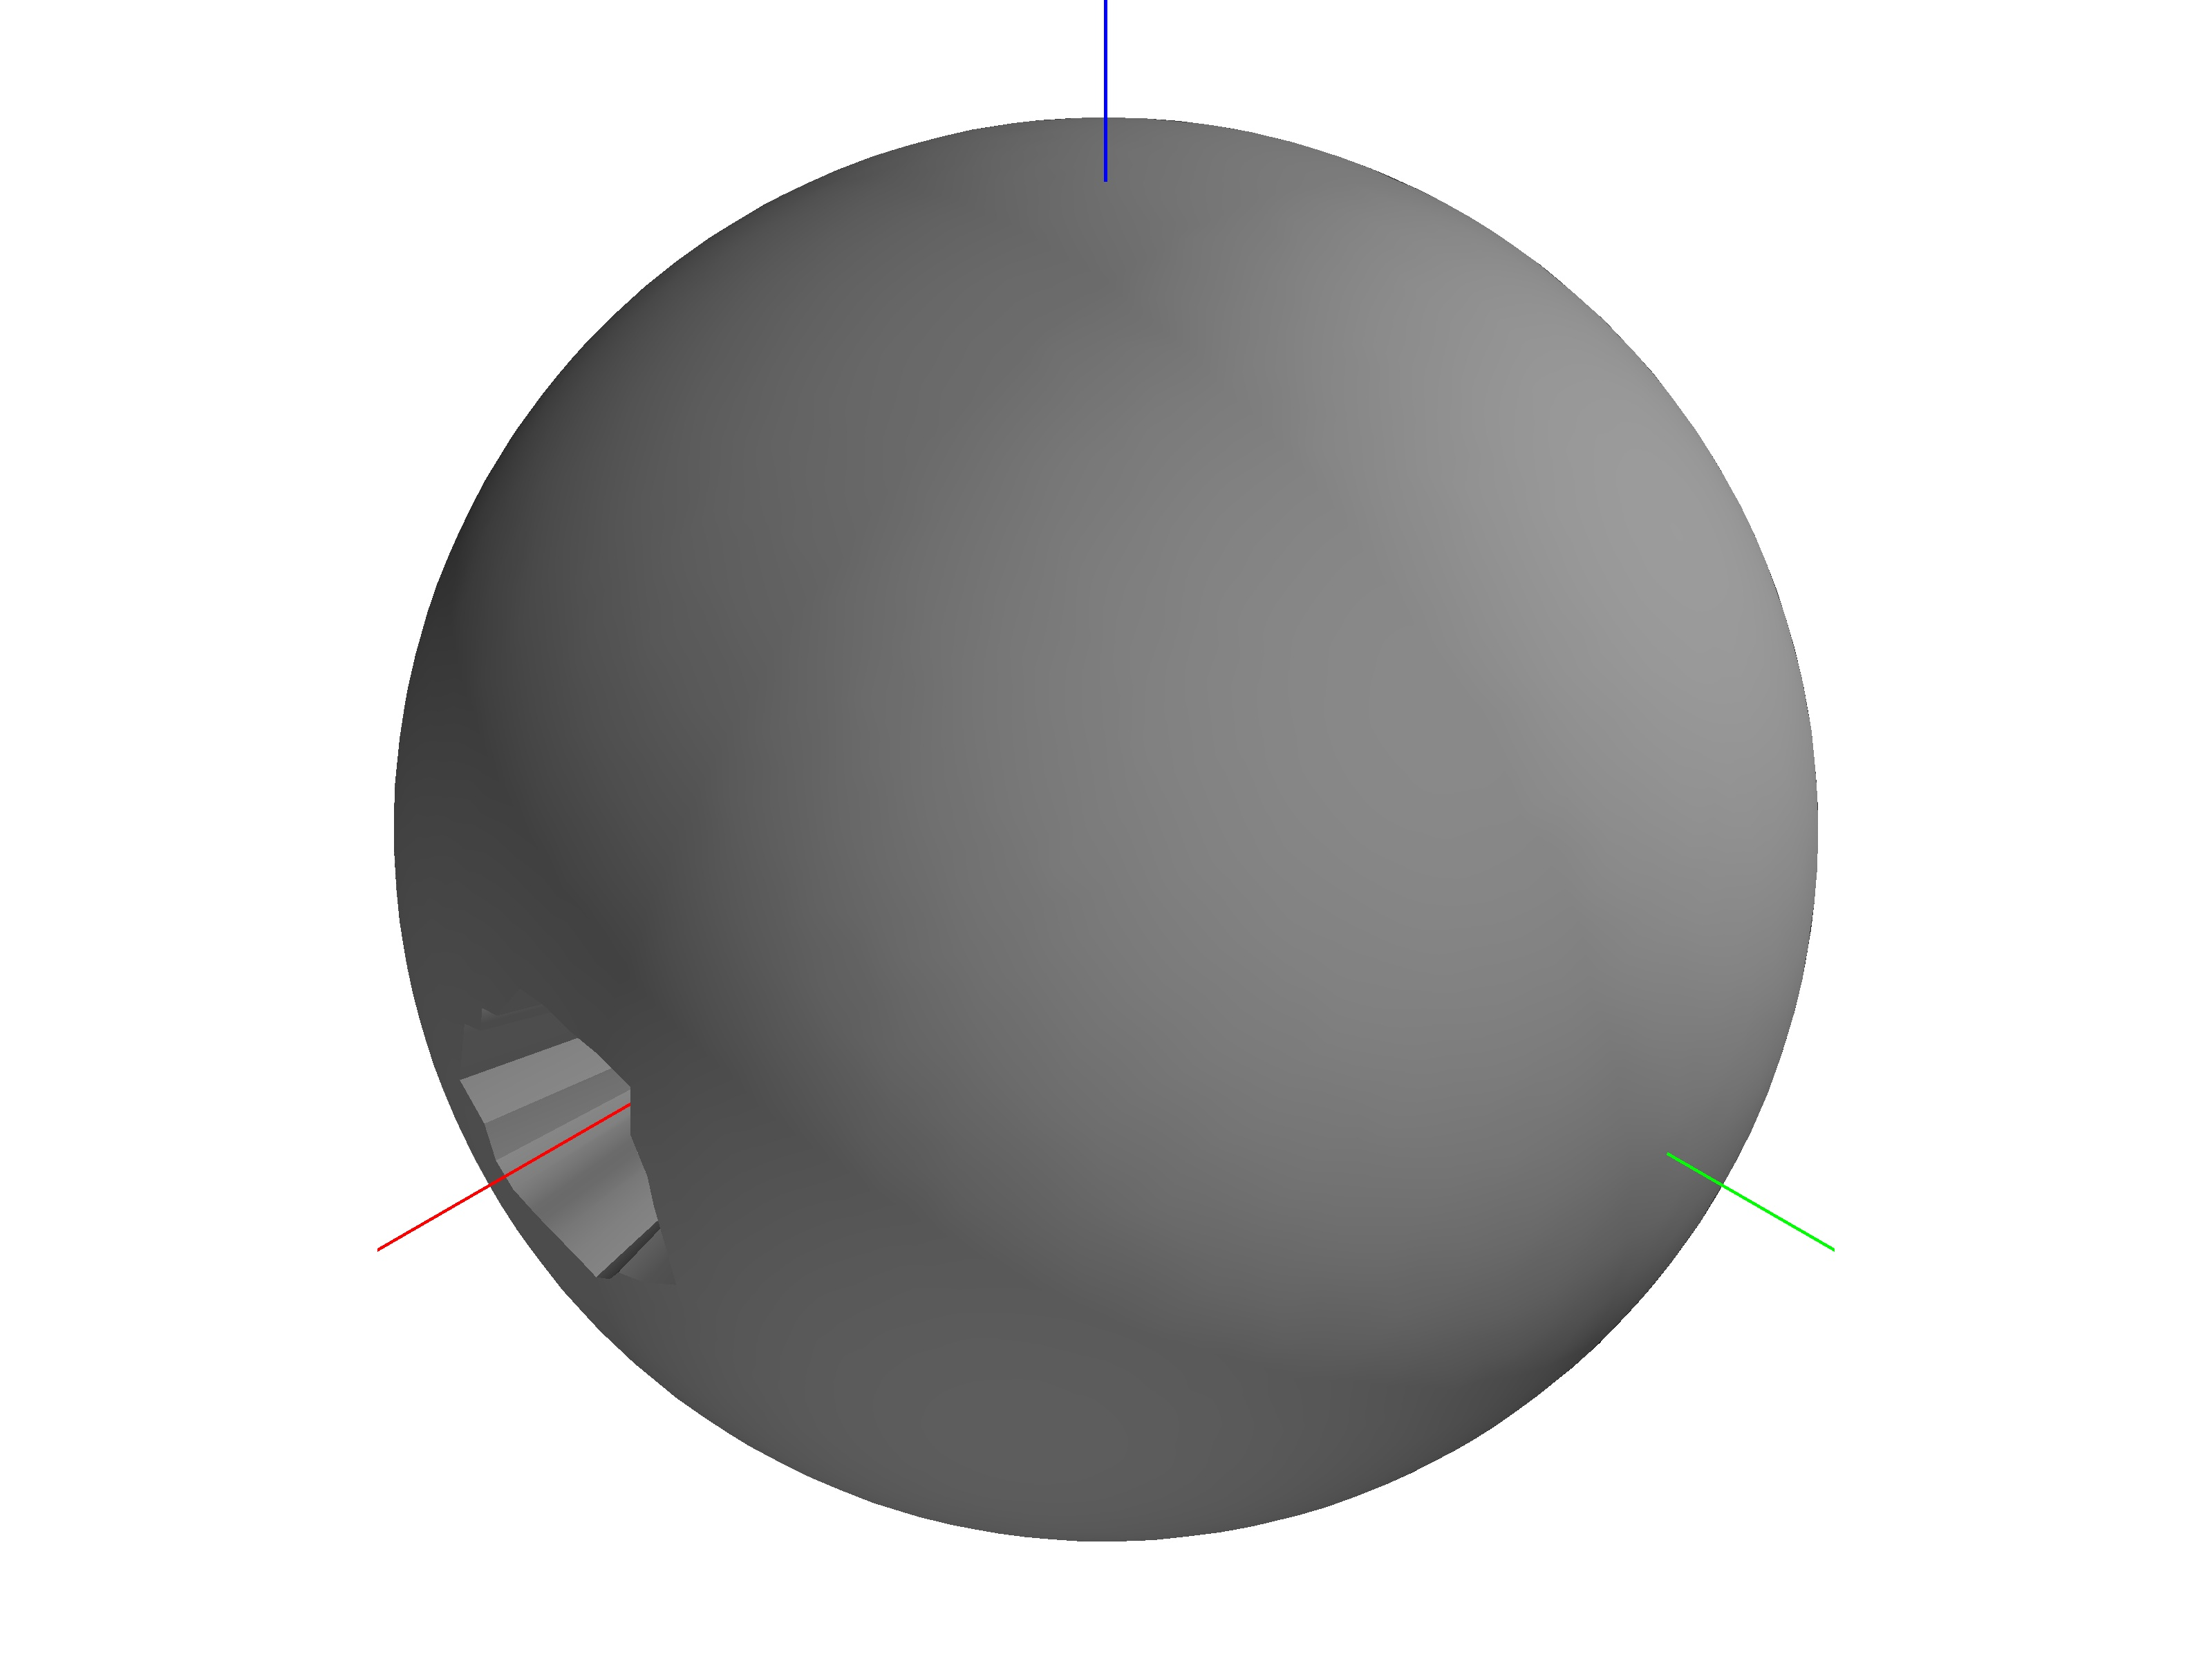
\includegraphics[height=0.5\textheight,width=0.5\textwidth,keepaspectratio]{figures/computational_geometry/mesh_update/golevka/partial_0.jpg}}~
    \subcaptionbox{\SI{25}{\percent} of measurements added\label{fig:golevka_partial_25}}{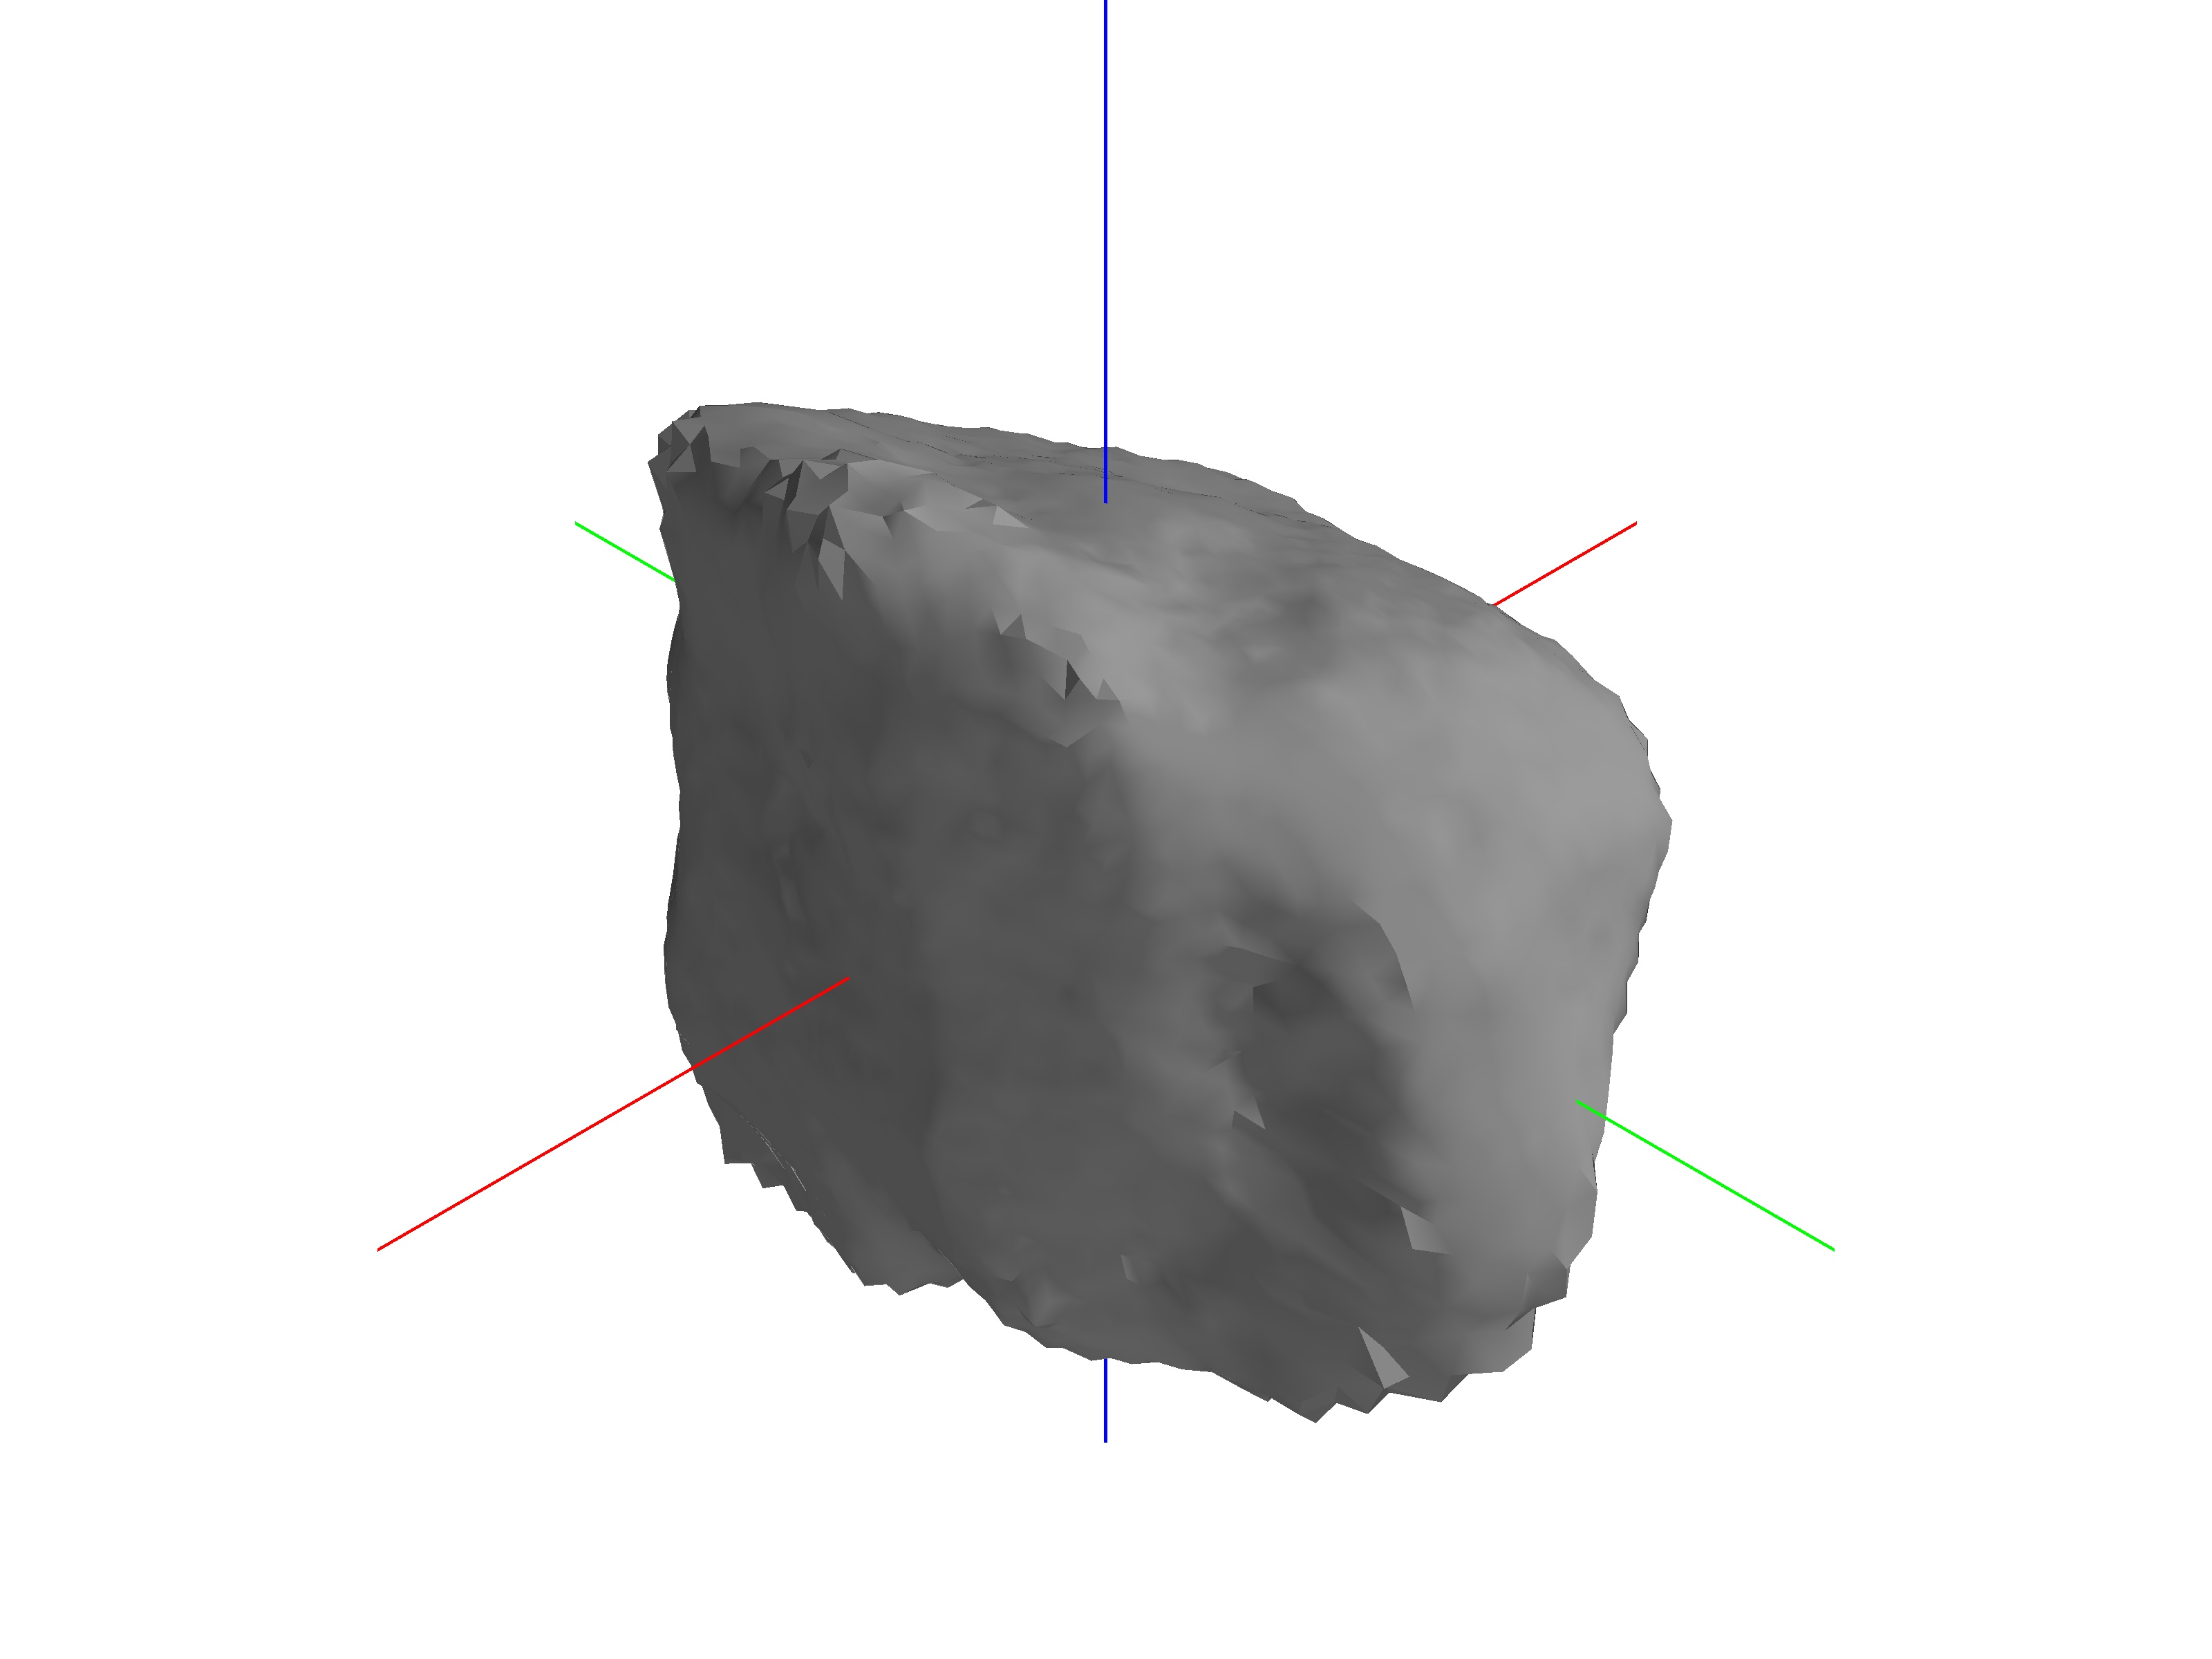
\includegraphics[width=0.5\textwidth]{figures/computational_geometry/mesh_update/golevka/partial_1321.jpg}}

    \subcaptionbox{\SI{50}{\percent} of measurments added\label{fig:golevka_partial_50}}{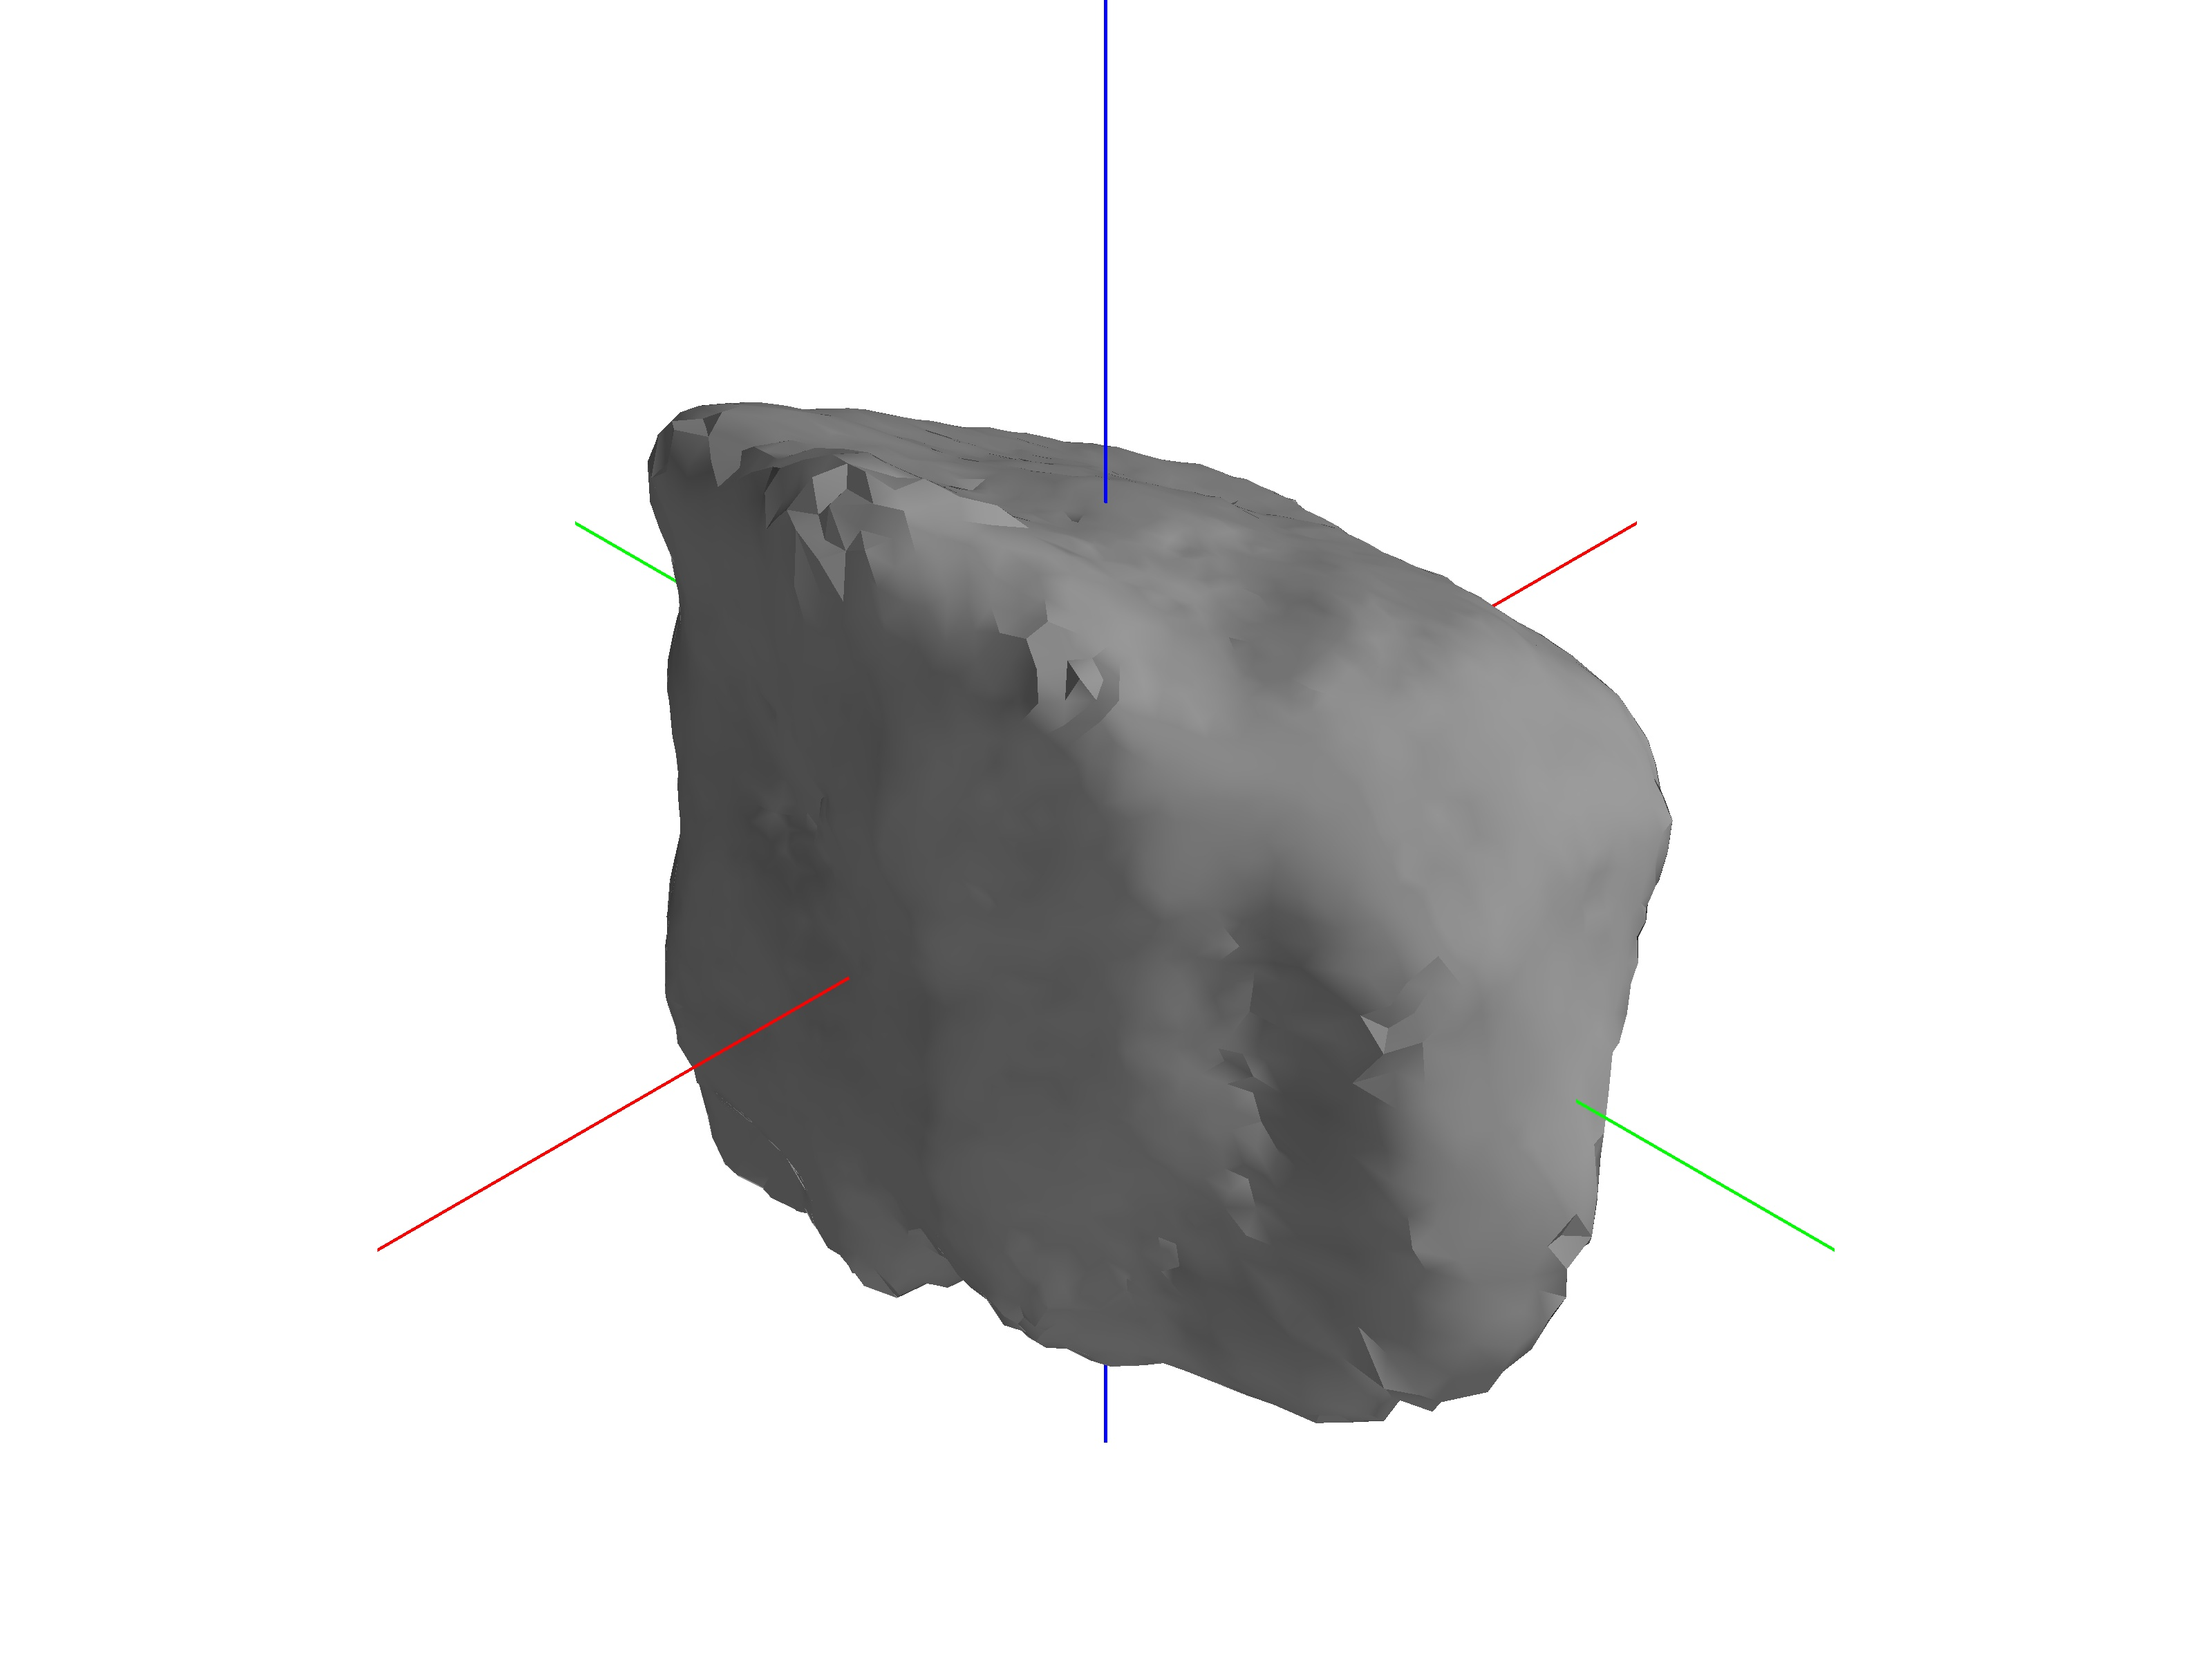
\includegraphics[width=0.5\textwidth]{figures/computational_geometry/mesh_update/golevka/partial_2643.jpg}}~
    \subcaptionbox{\SI{75}{\percent} of measurements added\label{fig:golevka_partial_75}}{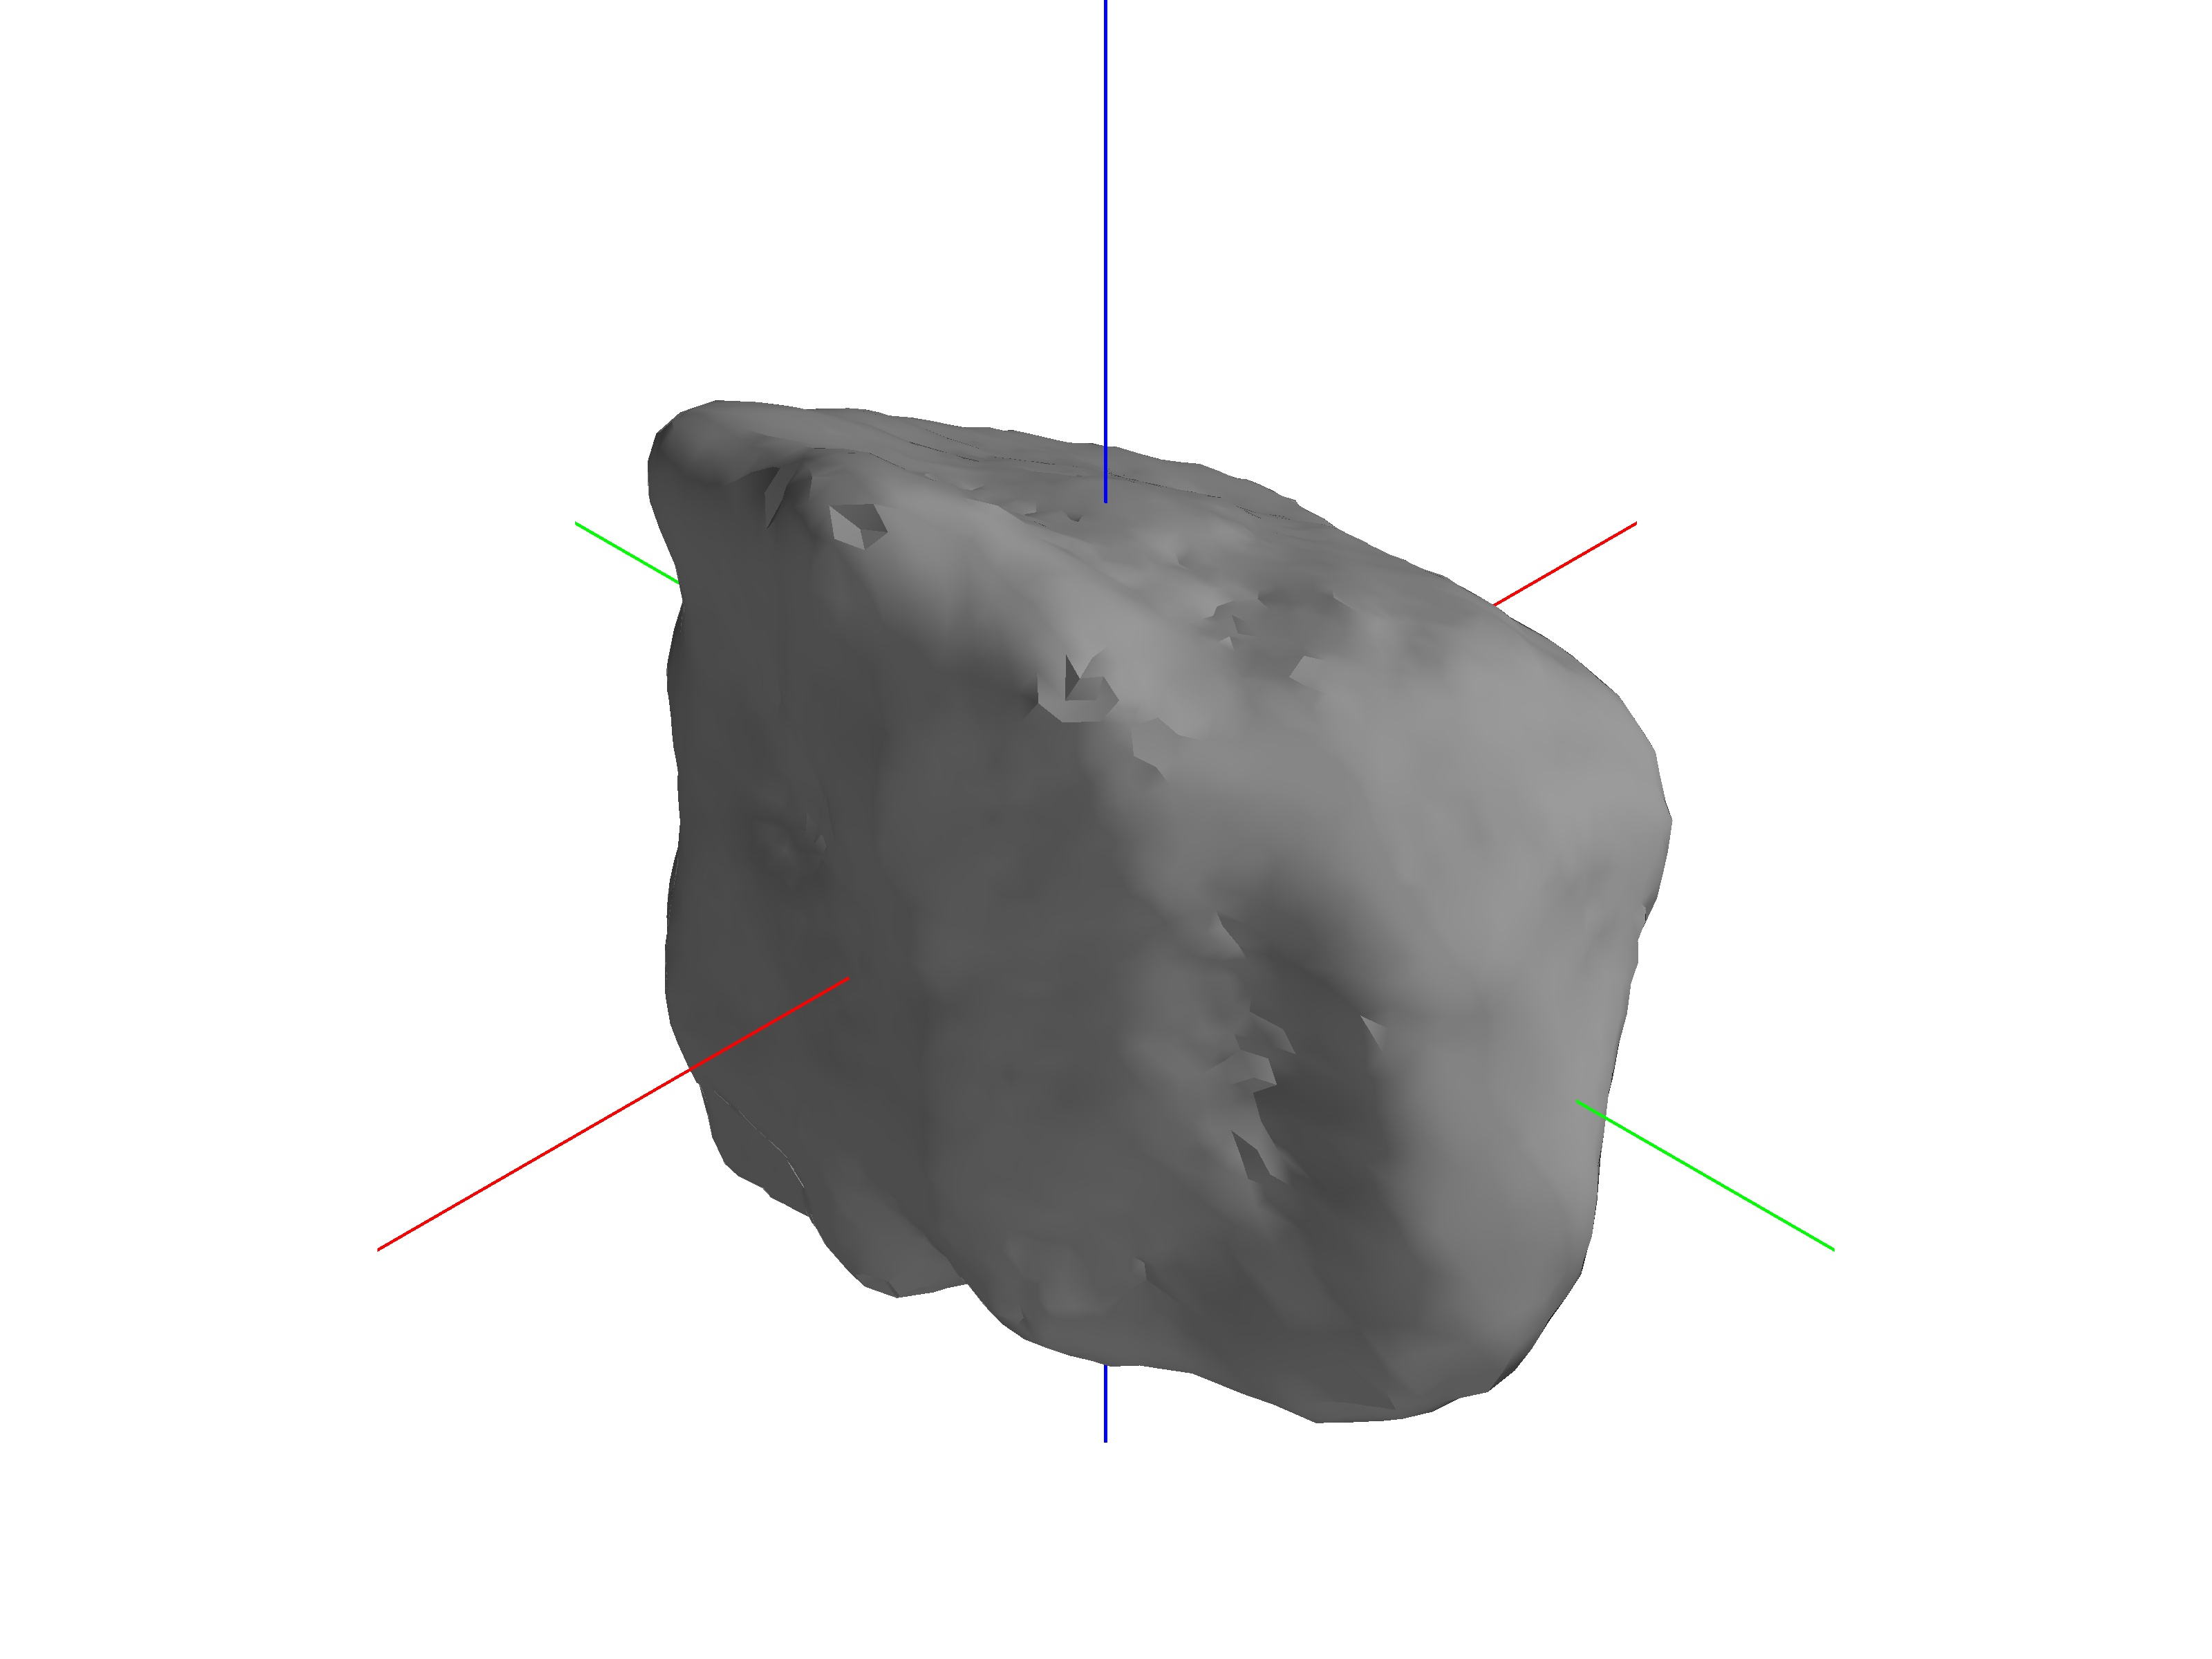
\includegraphics[width=0.5\textwidth]{figures/computational_geometry/mesh_update/golevka/partial_3964.jpg}}

    \subcaptionbox{\SI{100}{\percent} of measurements added\label{fig:golevka_partial_100}}{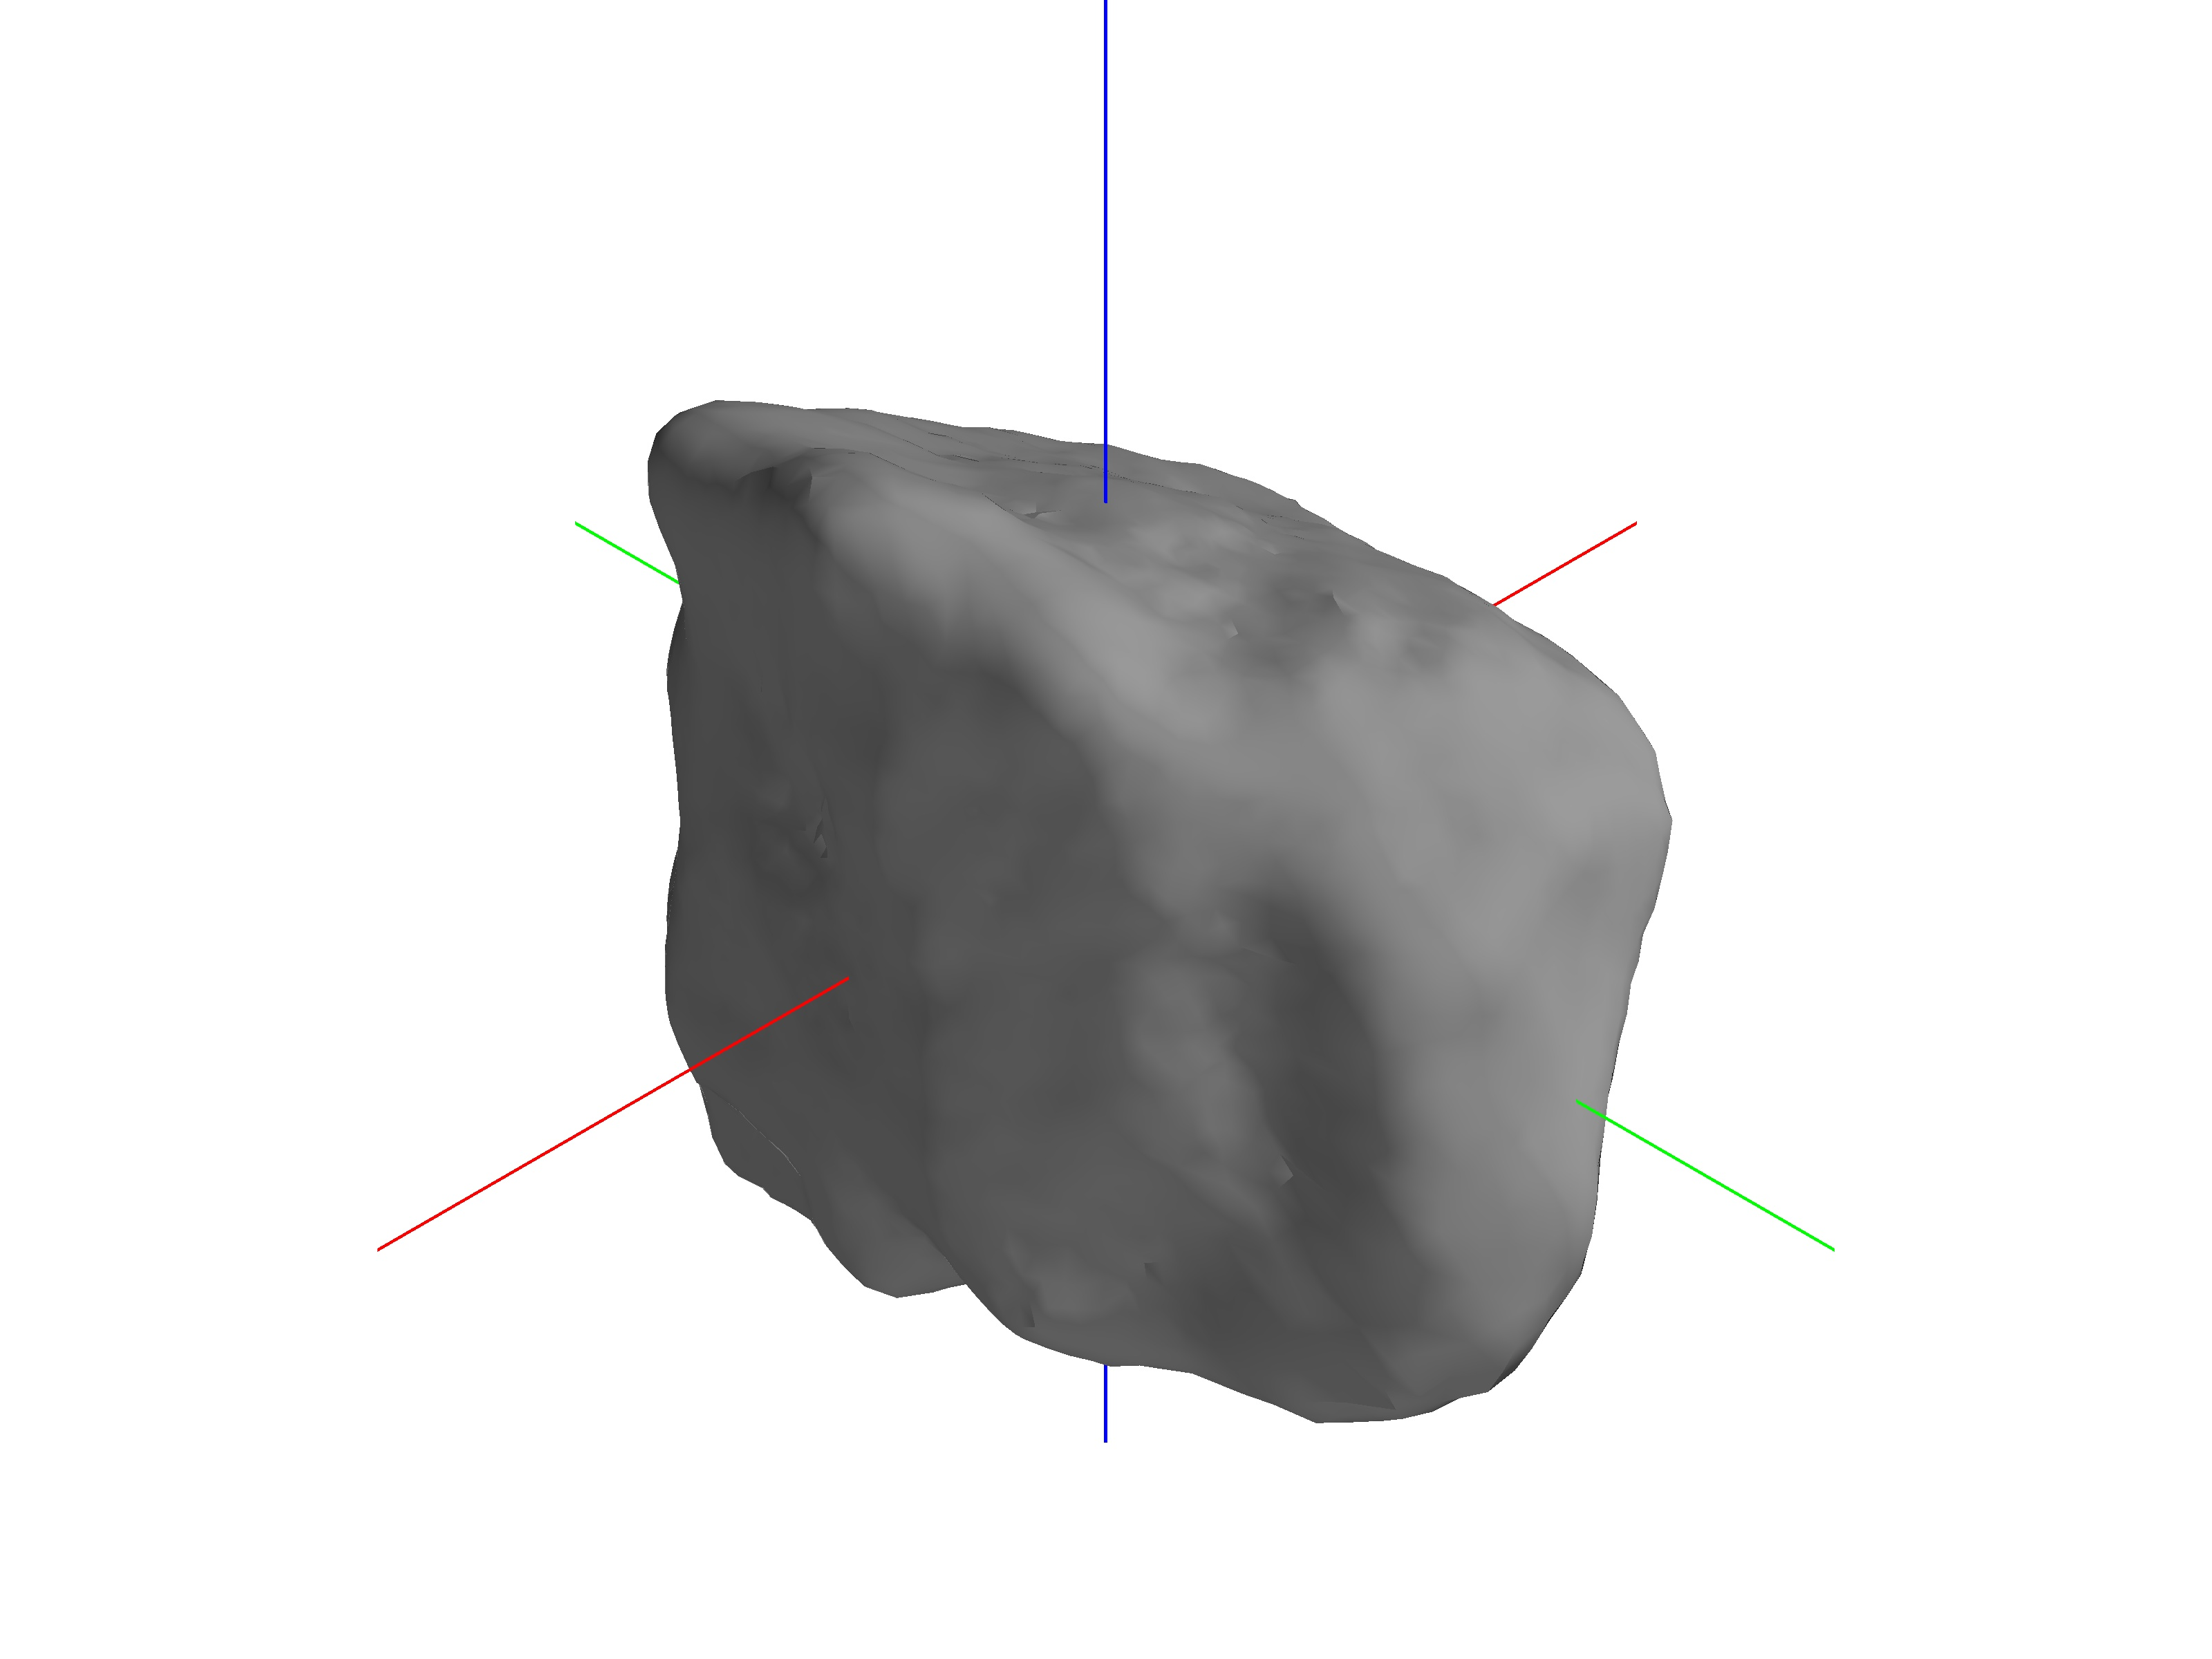
\includegraphics[width=0.5\textwidth]{figures/computational_geometry/mesh_update/golevka/partial_5285.jpg}}~
    \subcaptionbox{True Shape Model\label{fig:golevka_truth}}{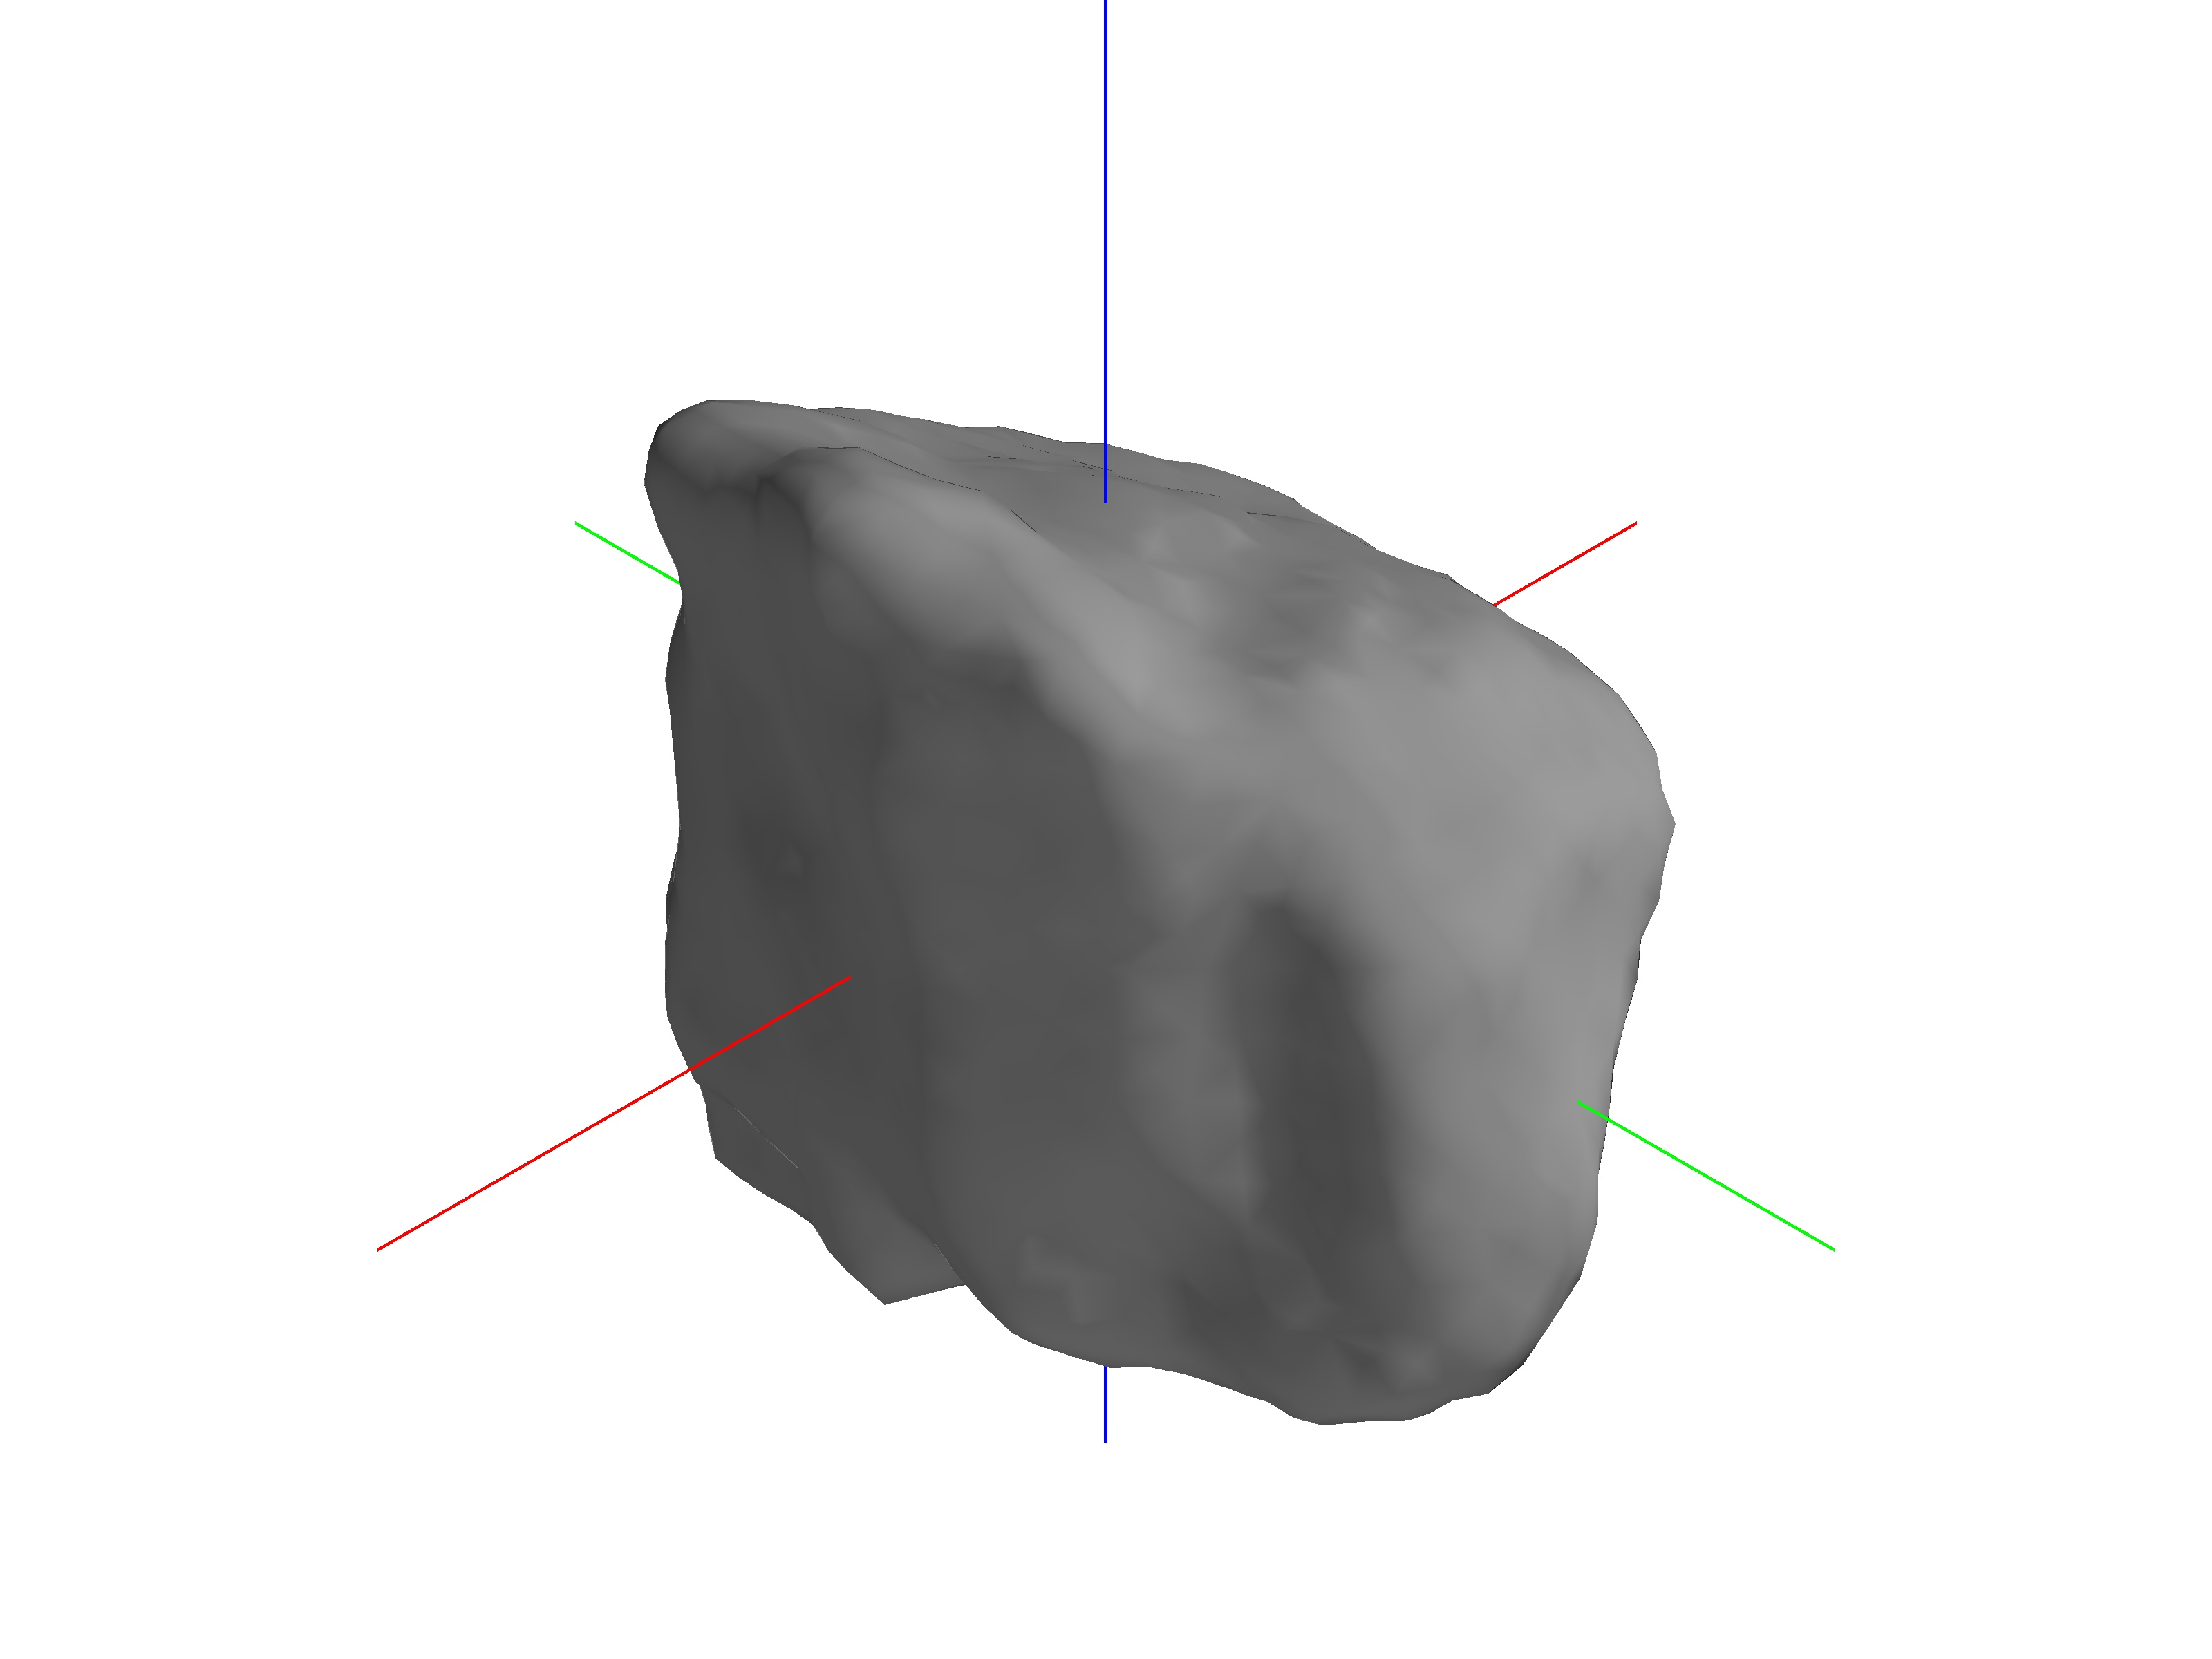
\includegraphics[width=0.5\textwidth]{figures/computational_geometry/mesh_update/golevka/truth.jpg}}
    \caption[Asteroid Golevka Incremental Reconstruction]{Incremental Reconstruction of asteroid Golevka~\label{fig:golevka_reconstruction}}
\end{figure}

\subsection{Full Dynamic Model }\label{sec:dynamic_exploration}
In this section, we simulate a dumbbell spacecraft in motion around asteroid \num{52760} and asteroid Castalia.
The dynamic simulation utilizes the inertial equations of motion from~\cref{sec:inertial_dumbbell_eoms} and are given as
\begin{align*}
    \dot{\ipos} &= \ivel, \\
    \parenth{m_1 + m_2} \dot{\ivel} &= - \sum_{i=0}^2 m_i \aatt \deriv{U}{\apos_i} + u_f, \\
    \dot{\iatt} &= \iatt \iangvel, \label{eq:inertial_attitude_dynamics}\\
    J \dot{\iangvel} + \hat{\iangvel} J \iangvel &= \sum_{i=0}^2 m_i \hat{\spos}_i \iatt^T \aatt \deriv{U}{\apos_i} + u_m. 
\end{align*}
The nonlinear controllers described in~\cref{sec:se3_control} are used to control both the translational and rotational states of the vehicle.
The control inputs are duplicated from~\cref{sec:se3_control} as
\begin{align*}
    \vc{u}_f &= -k_x e_x - k_v e_v - F_{ext} + m \ddot{x}_d . \\
    \vc{u}_m &= -k_R e_R - k_\Omega e_\Omega + \Omega \times J \Omega - M_{ext}.
\end{align*}
Throughout the simulation the control inputs are computed using the current shape estimate of the asteroid. 
As measurements are collected, the spacecraft autonomously updates its shape estimate and uses this estimate to compute the control inputs and desired future states.

We consider two simulations about asteroids \num{52760} and Castalia.
The asteroids are assumed to constantly rotate about the \( \vc{f}_3 = \vc{e}_3\) axis according to the parameters given in~\cref{tab:dynamic_asteroids}.
Furthermore, the state of the asteroid, namely the rotation matrix \( \aatt \), is assumed to be known based on ground measurements or previous data.
\begin{table}[htbp]
    \centering
    \begin{tabular}{lcc}
        \toprule
        Property & \num{4769} Castalia & (\num{52760}) \num{1998} \(\text{ML}_{14}\) \\
        \midrule
        Semi-major axes(\si{\kilo\meter}) & \( 0.8065 \times 0.4905 \times 0.413 \) & \( 1.1 \times 1.1 \times 1.1 \) \\
        Rotational Period (\si{\hour}) & \num{4.095} & \num{14.98} \\
        Density (\si{\gram\per\centi\meter^3}) & \num{2.1} & \num{2.1} \\
        Vertices & \num{2048}  & \num{8192} \\
        Faces & \num{4092} & \num{16320} \\
        \bottomrule
    \end{tabular}
    \caption{Asteroid properties for dynamic exploration~\label{tab:dynamic_asteroids}}
\end{table}
At the beginning of the simulation the spacecraft is assumed to lie on the inertial \( e_1 \) axis, i.e.\ \( \ipos(0) = \begin{bmatrix} x_0 & 0 & 0 \end{bmatrix} \si{\kilo\meter} \).
In addition, at the initial state the spacecraft is orientated such that the \( b_1 \) axis is aligned with the inertial \( e_2 \) axis.
In other words the initial orientation is given by \( \iatt(0) = \exp(\frac{\pi}{2} \hat{e}_3)\).
The shape reconstruction phase of the simulation is simulation over \SI{15000}{\second}, over which time the spacecraft will take \gls{lidar} measurements of the surface at \SI{1}{\hertz}.
Once the total uncertainty has been reduced sufficiently the spacecraft manuevers to a ``home'' position aligned with the \( f_1 \) axis of the asteroid.

\paragraph{Asteroid 52760 Reconstruction}
% TODO 52760 asteroid - show reconstruction, state trajectory, uncertainty and volume
Asteroid (\num{52760}) \num{1998} \(\text{ML}_{14}\) was discovered in \num{1998} and is near Earth asteroid of the Apollo group and classified as a potentially hazardous body.
The asteroid is roughly spherical with a mean radius of approximately \SI{1}{\kilo\meter}.
The initial shape estimate is assumed to be spherical with approximately the same number of vertices as the truth model.
\Cref{fig:52760_reconstruction,fig:52760_weights_reconstruction} show the shape reconstruction at several discrete points during the simulation.
Due to the roughly spherical shape of the asteorid large portions of the surface are quickly modified to match the measurements.
In addition~\cref{fig:52760_weights_reconstruction} displays the vertex uncertainty \( w_i \) as a colormap on the surface. 
Areas of high uncertainty are denoted in yellow while areas of low uncertainty are in purple/blue.

\begin{figure}[htbp]
    \centering
    \subcaptionbox{Initial Shape Estimate\label{fig:52760_partial_0}}{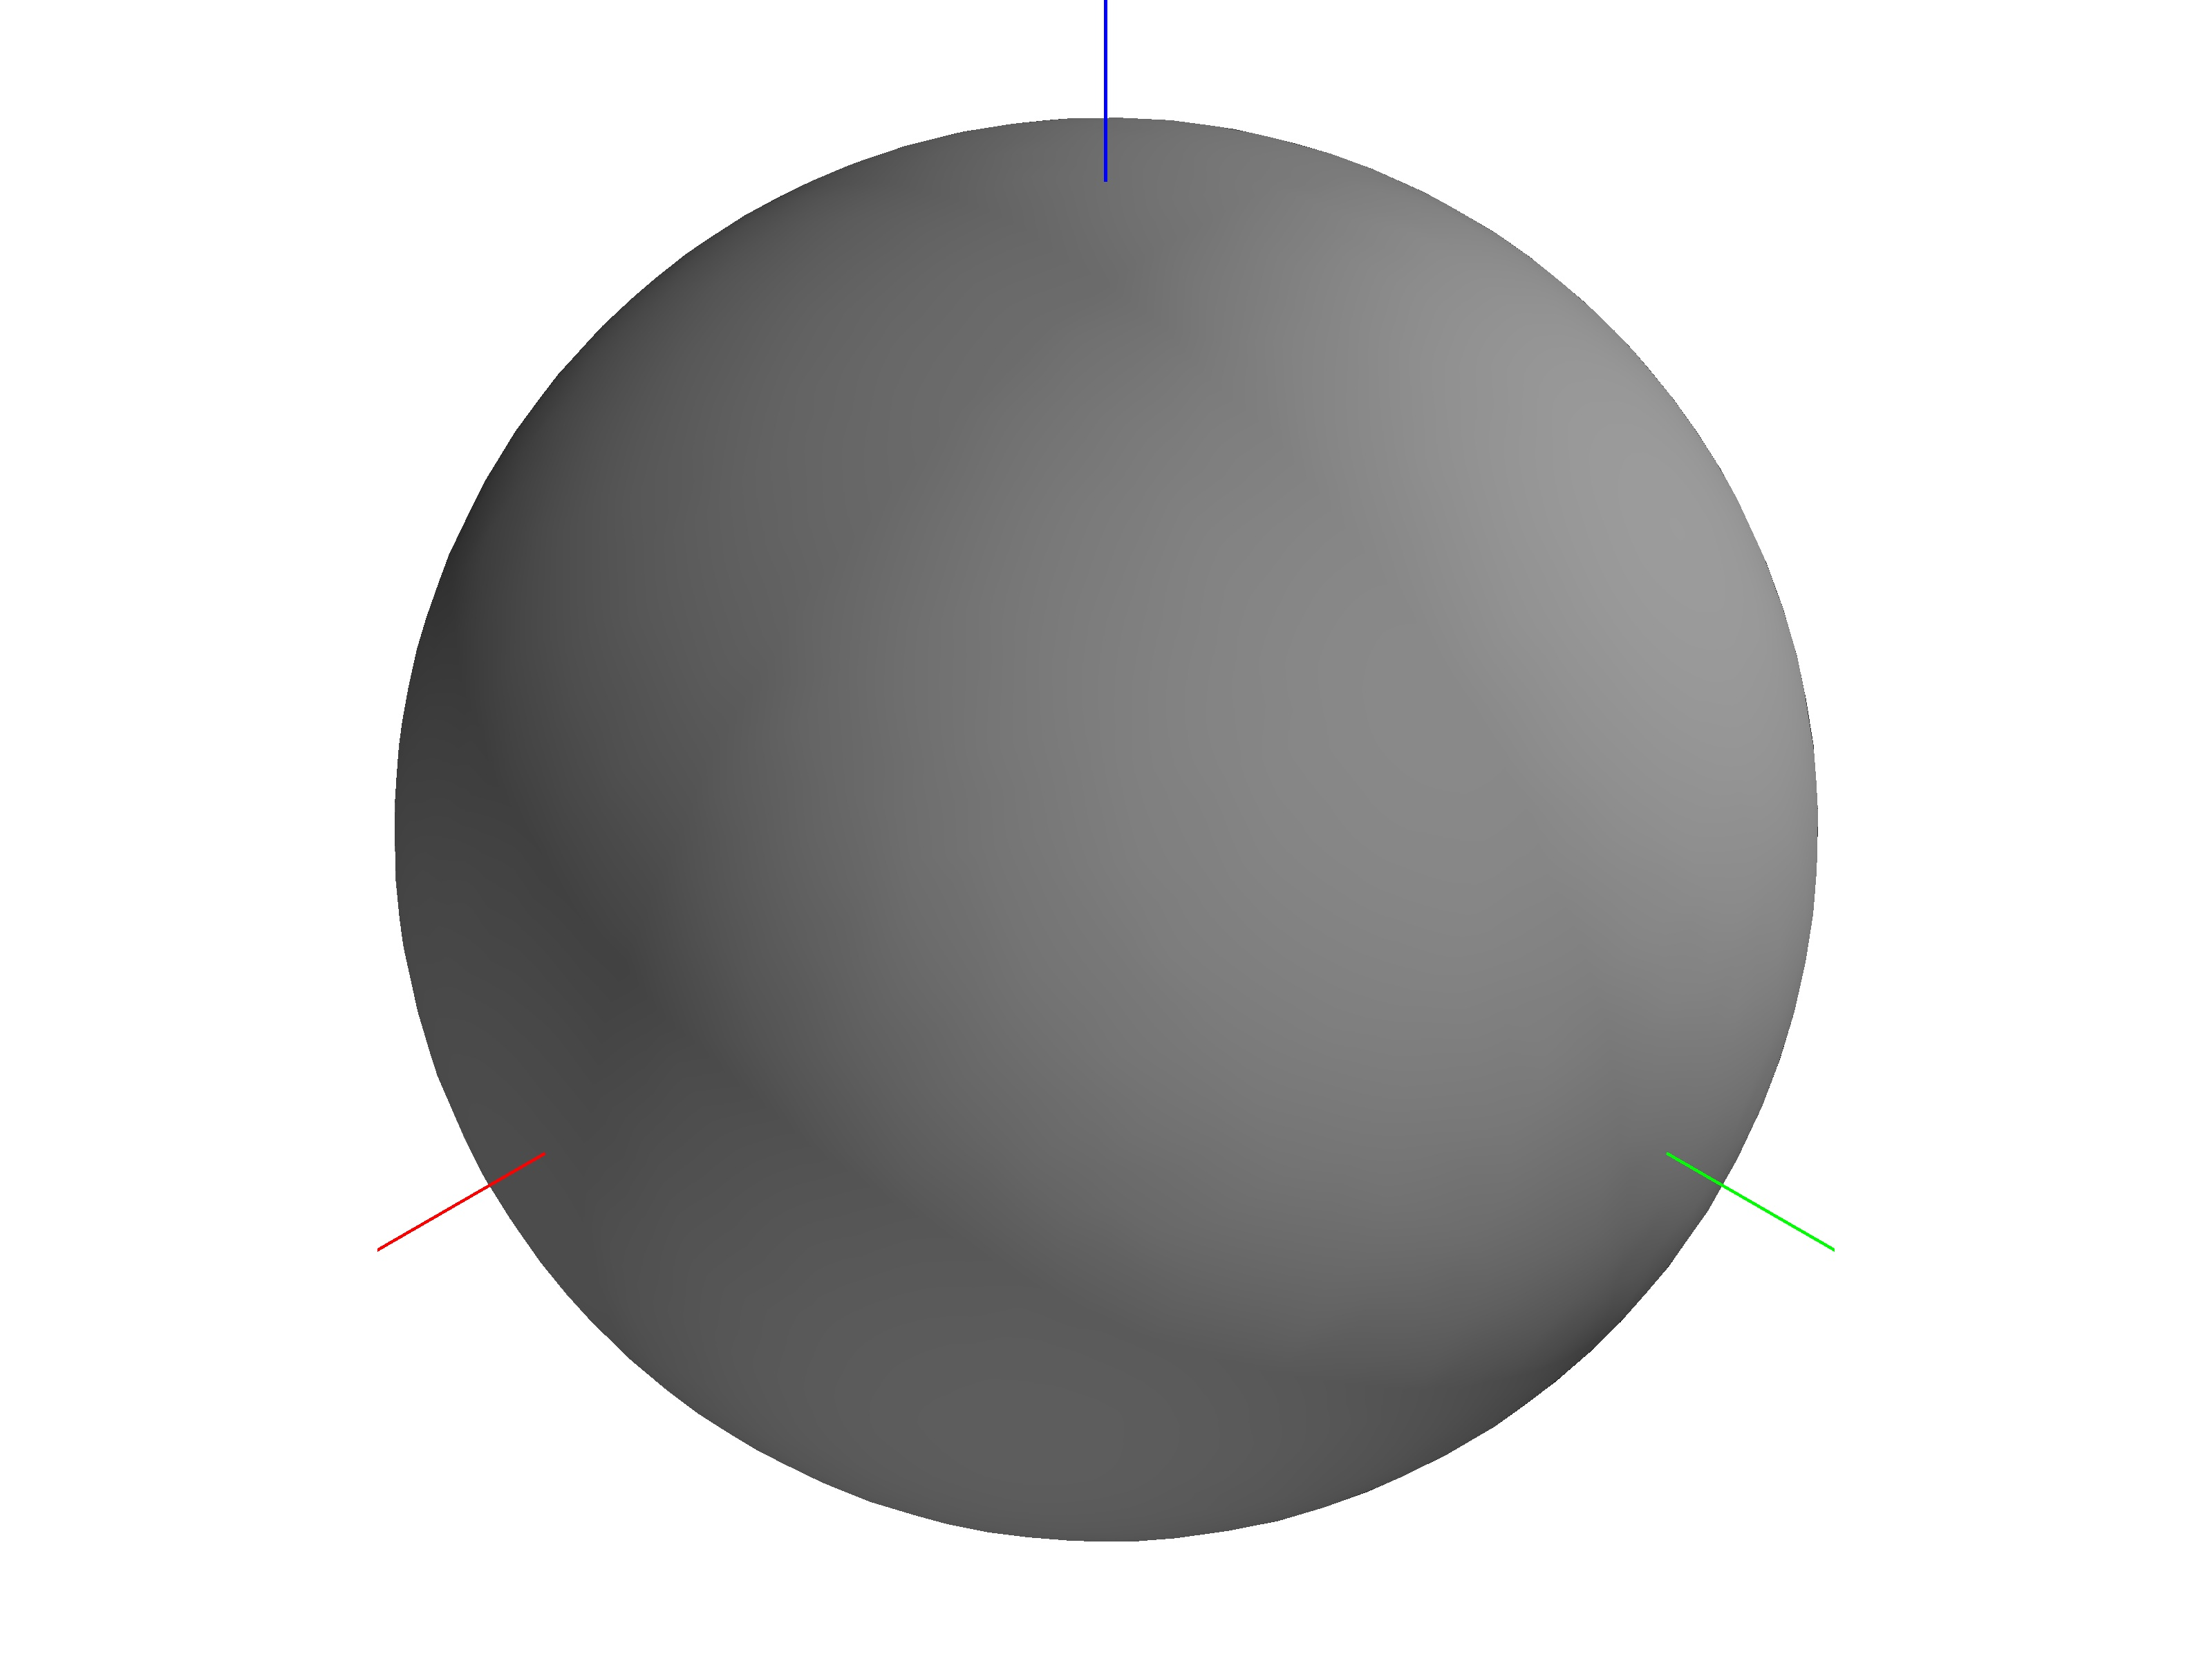
\includegraphics[height=0.5\textheight,width=0.5\textwidth,keepaspectratio]{figures/computational_geometry/dynamic_exploration/52760/partial_1.jpg}}~
    \subcaptionbox{\SI{25}{\percent} of measurements added\label{fig:52760_partial_25}}{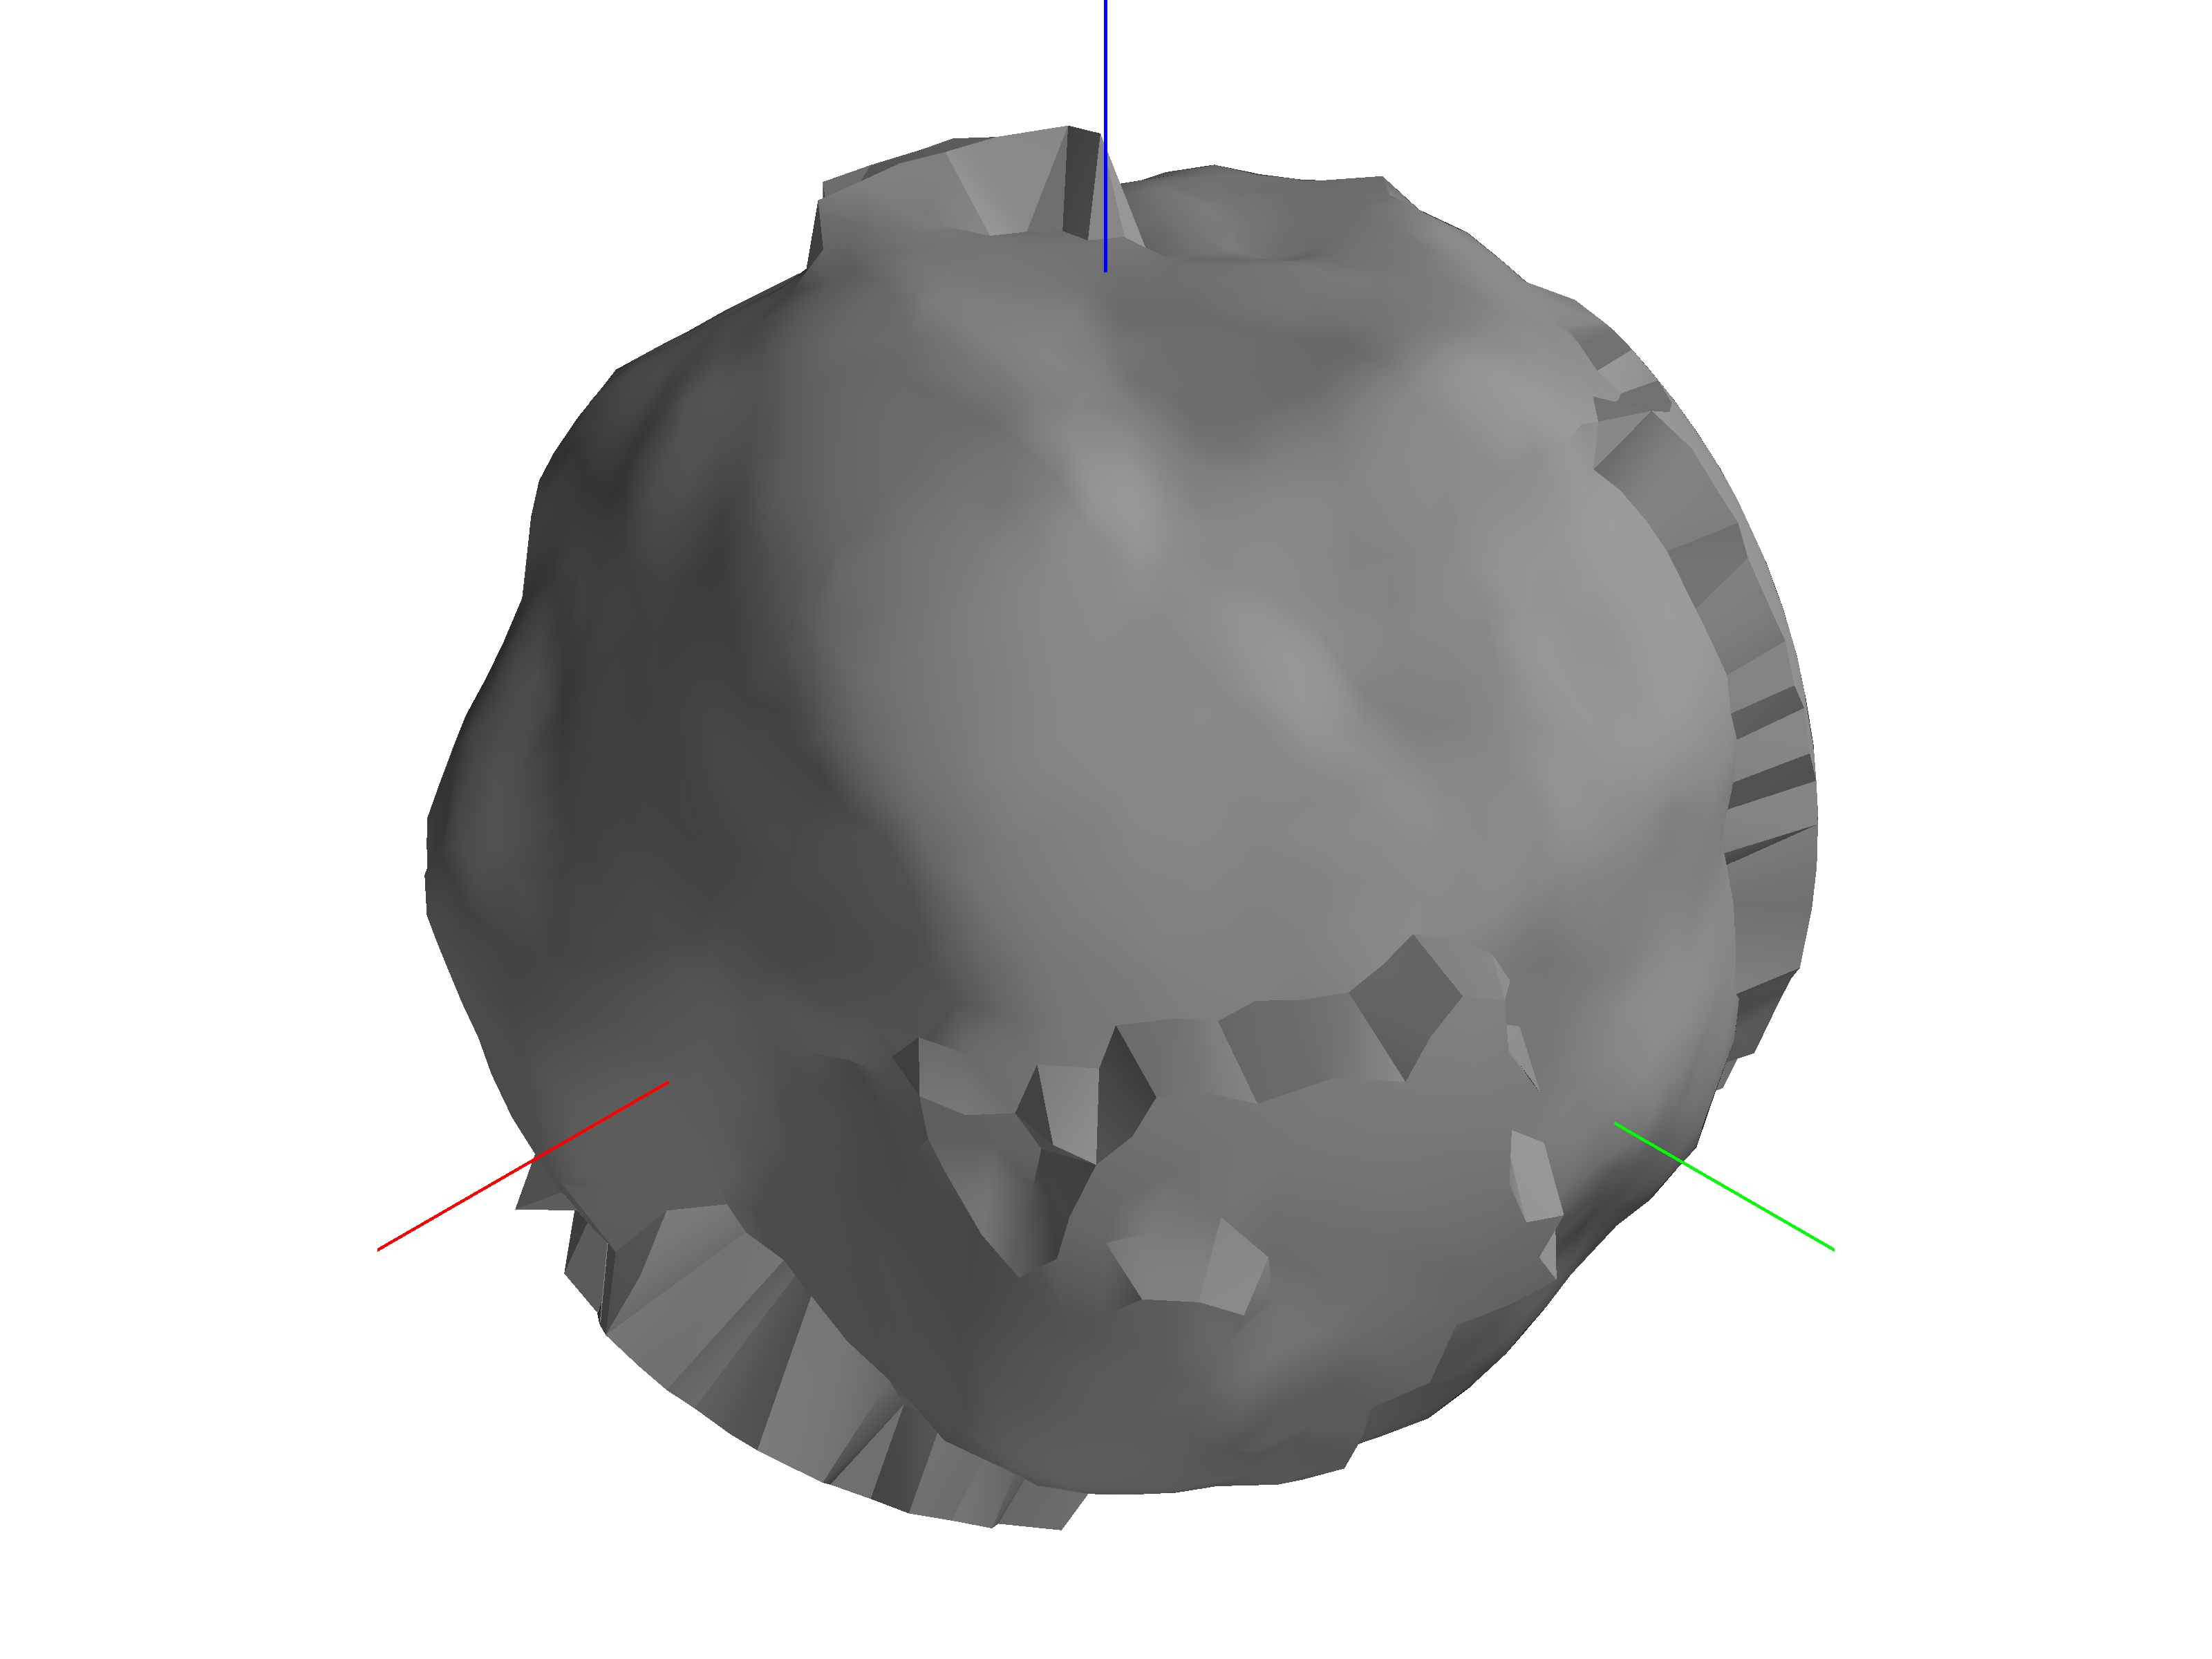
\includegraphics[width=0.5\textwidth]{figures/computational_geometry/dynamic_exploration/52760/partial_3749.jpg}}

    \subcaptionbox{\SI{50}{\percent} of measurments added\label{fig:52760_partial_50}}{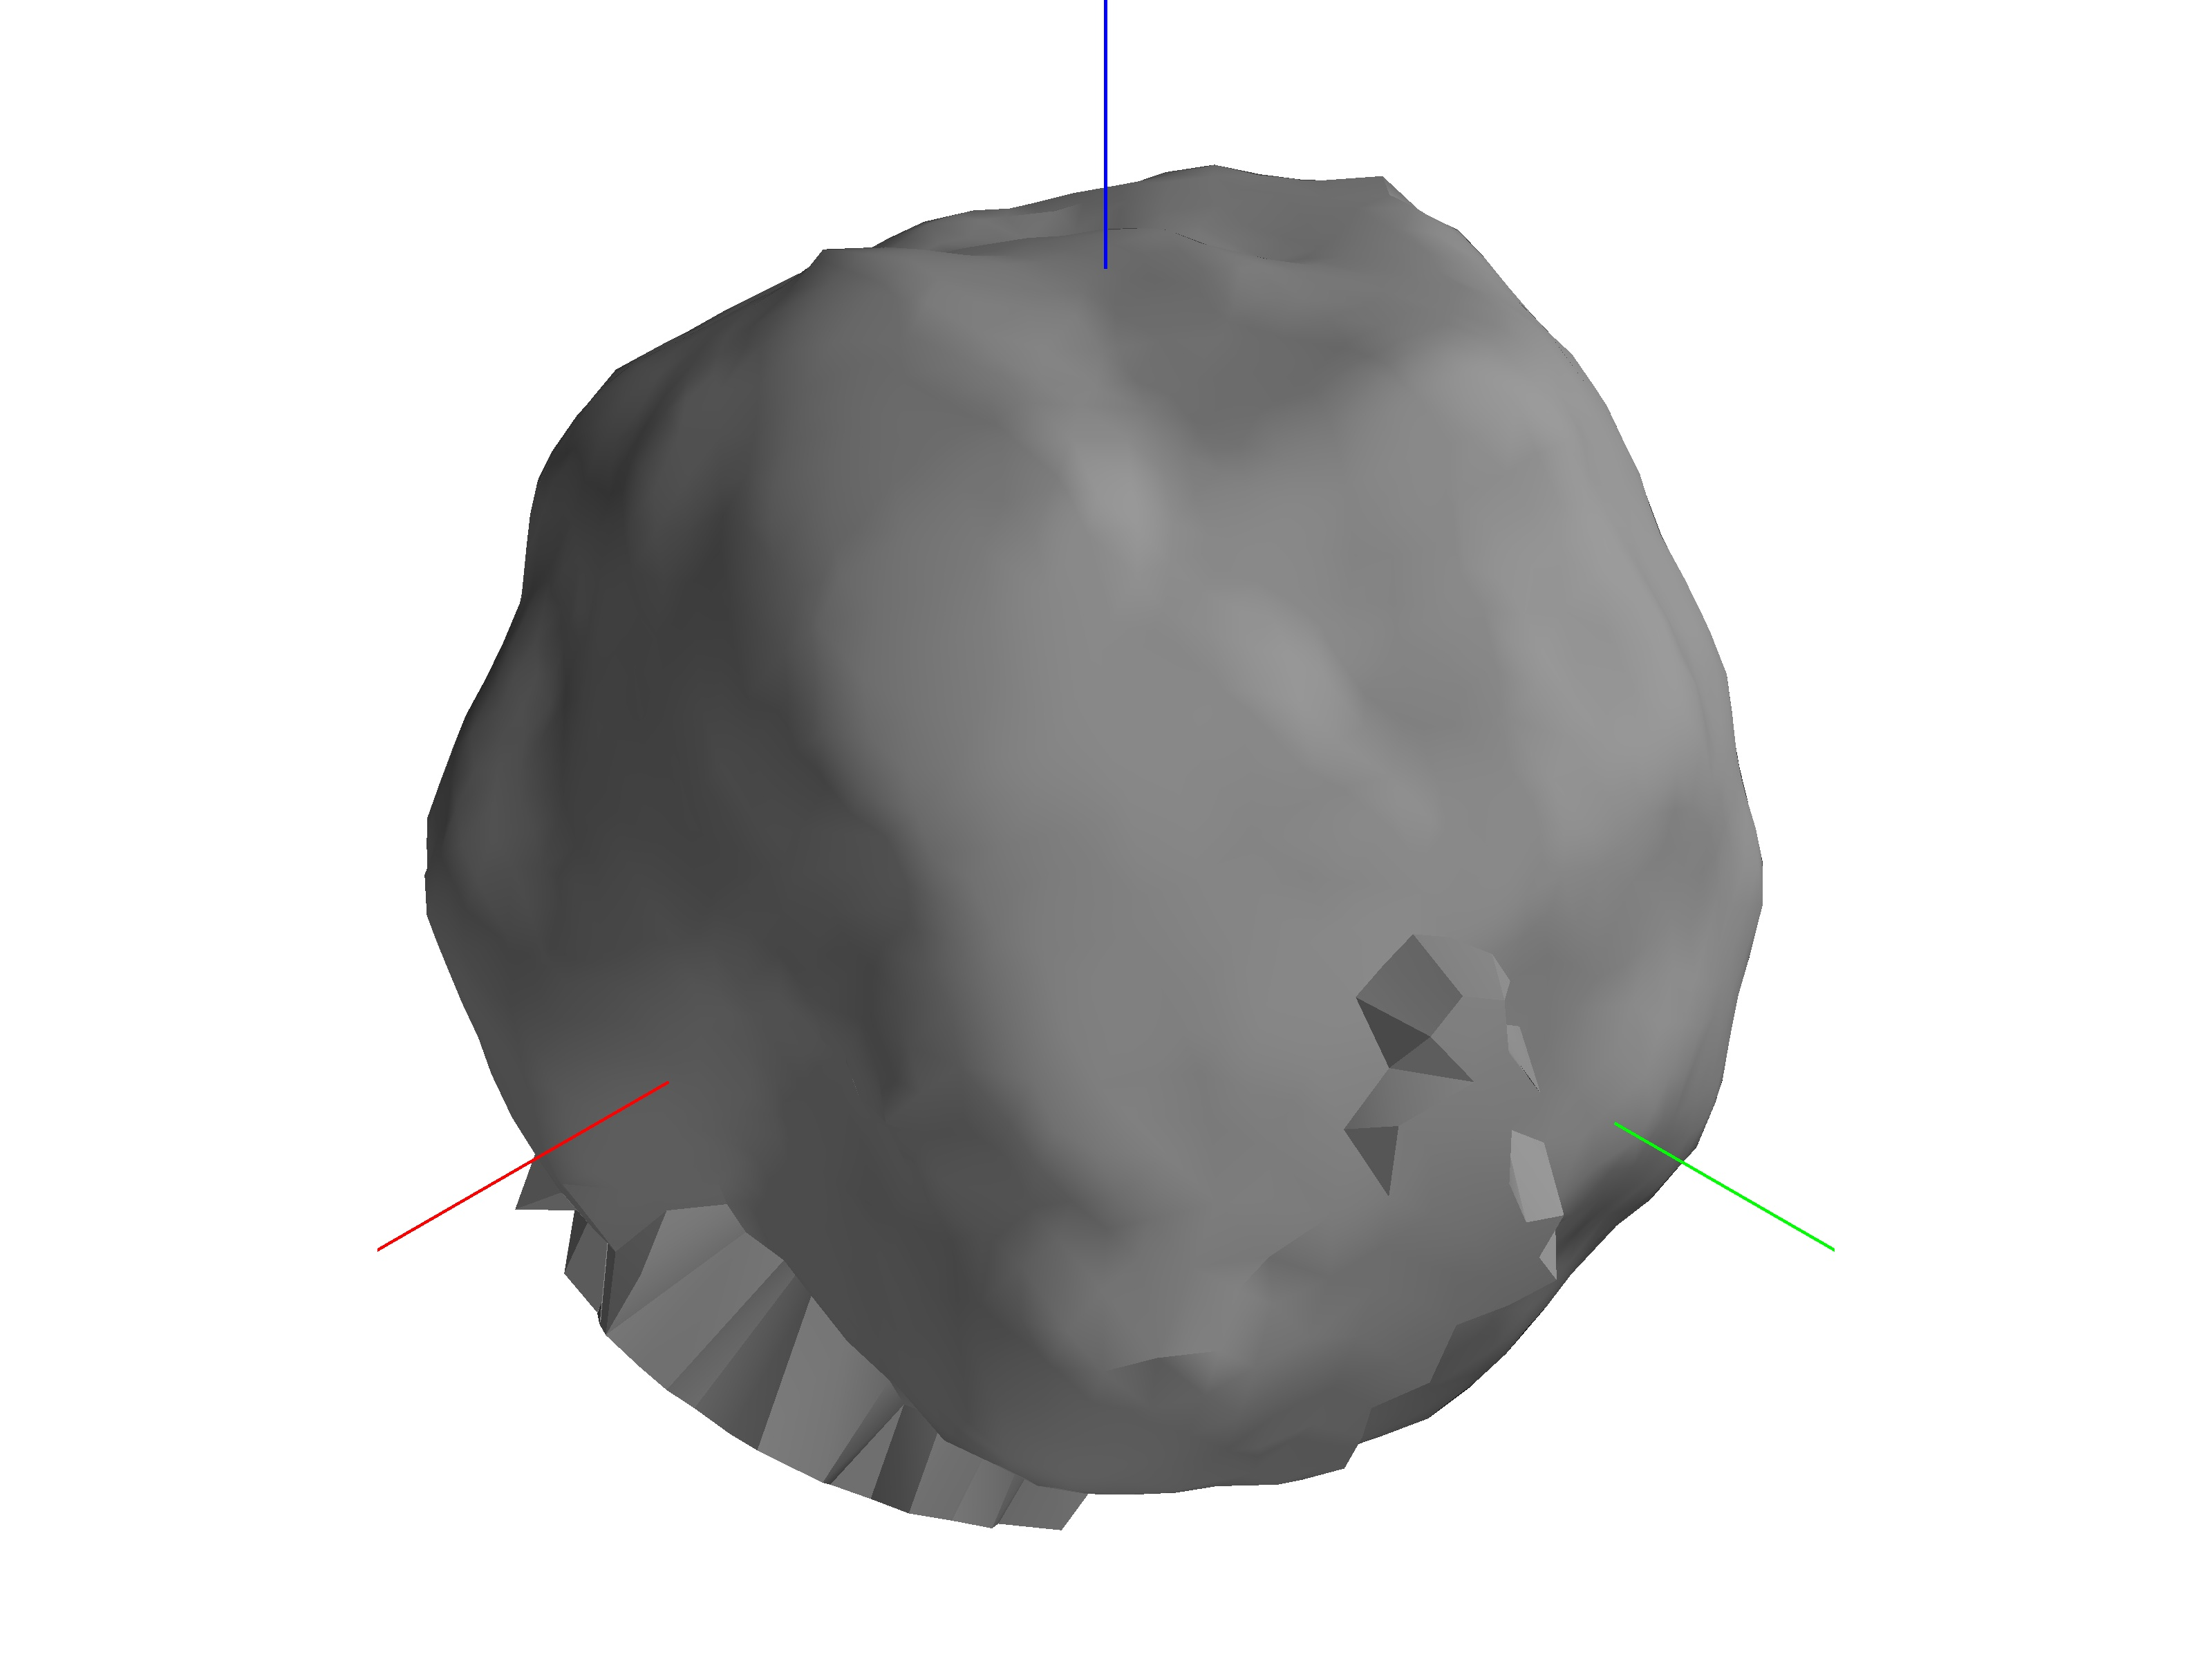
\includegraphics[width=0.5\textwidth]{figures/computational_geometry/dynamic_exploration/52760/partial_7499.jpg}}~
    \subcaptionbox{\SI{75}{\percent} of measurements added\label{fig:52760_partial_75}}{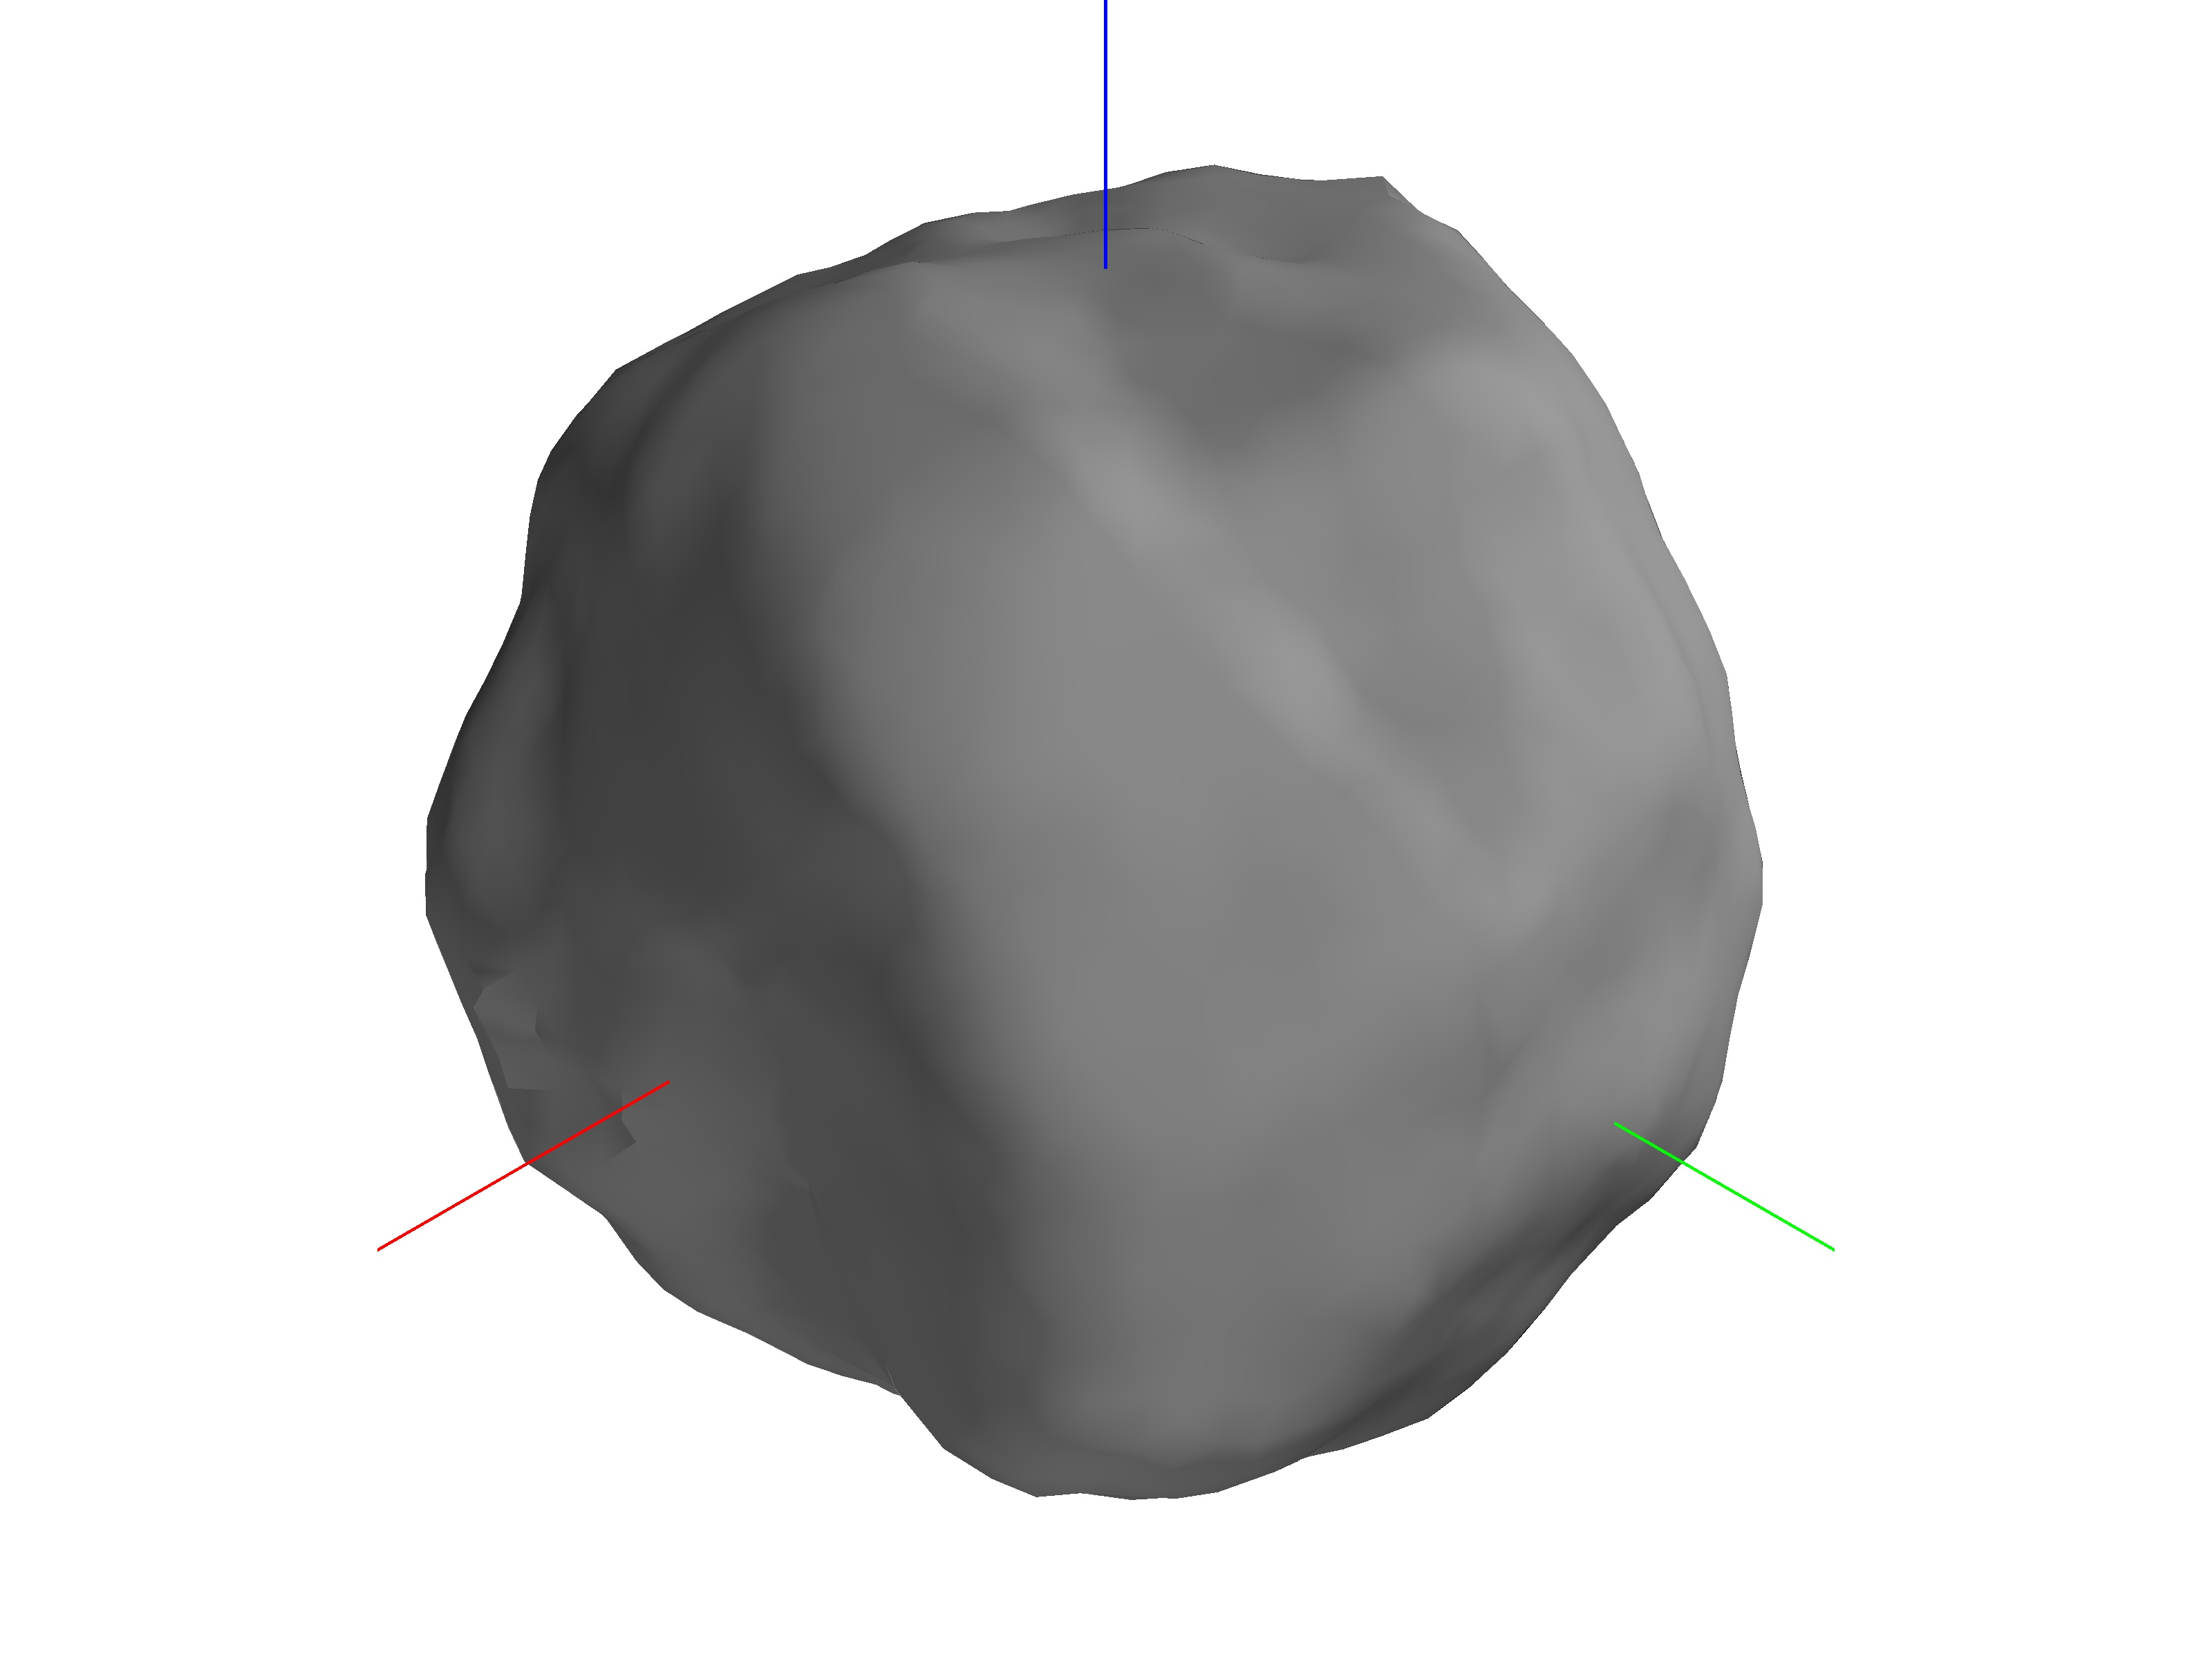
\includegraphics[width=0.5\textwidth]{figures/computational_geometry/dynamic_exploration/52760/partial_11249.jpg}}

    \subcaptionbox{\SI{100}{\percent} of measurements added\label{fig:52760_partial_100}}{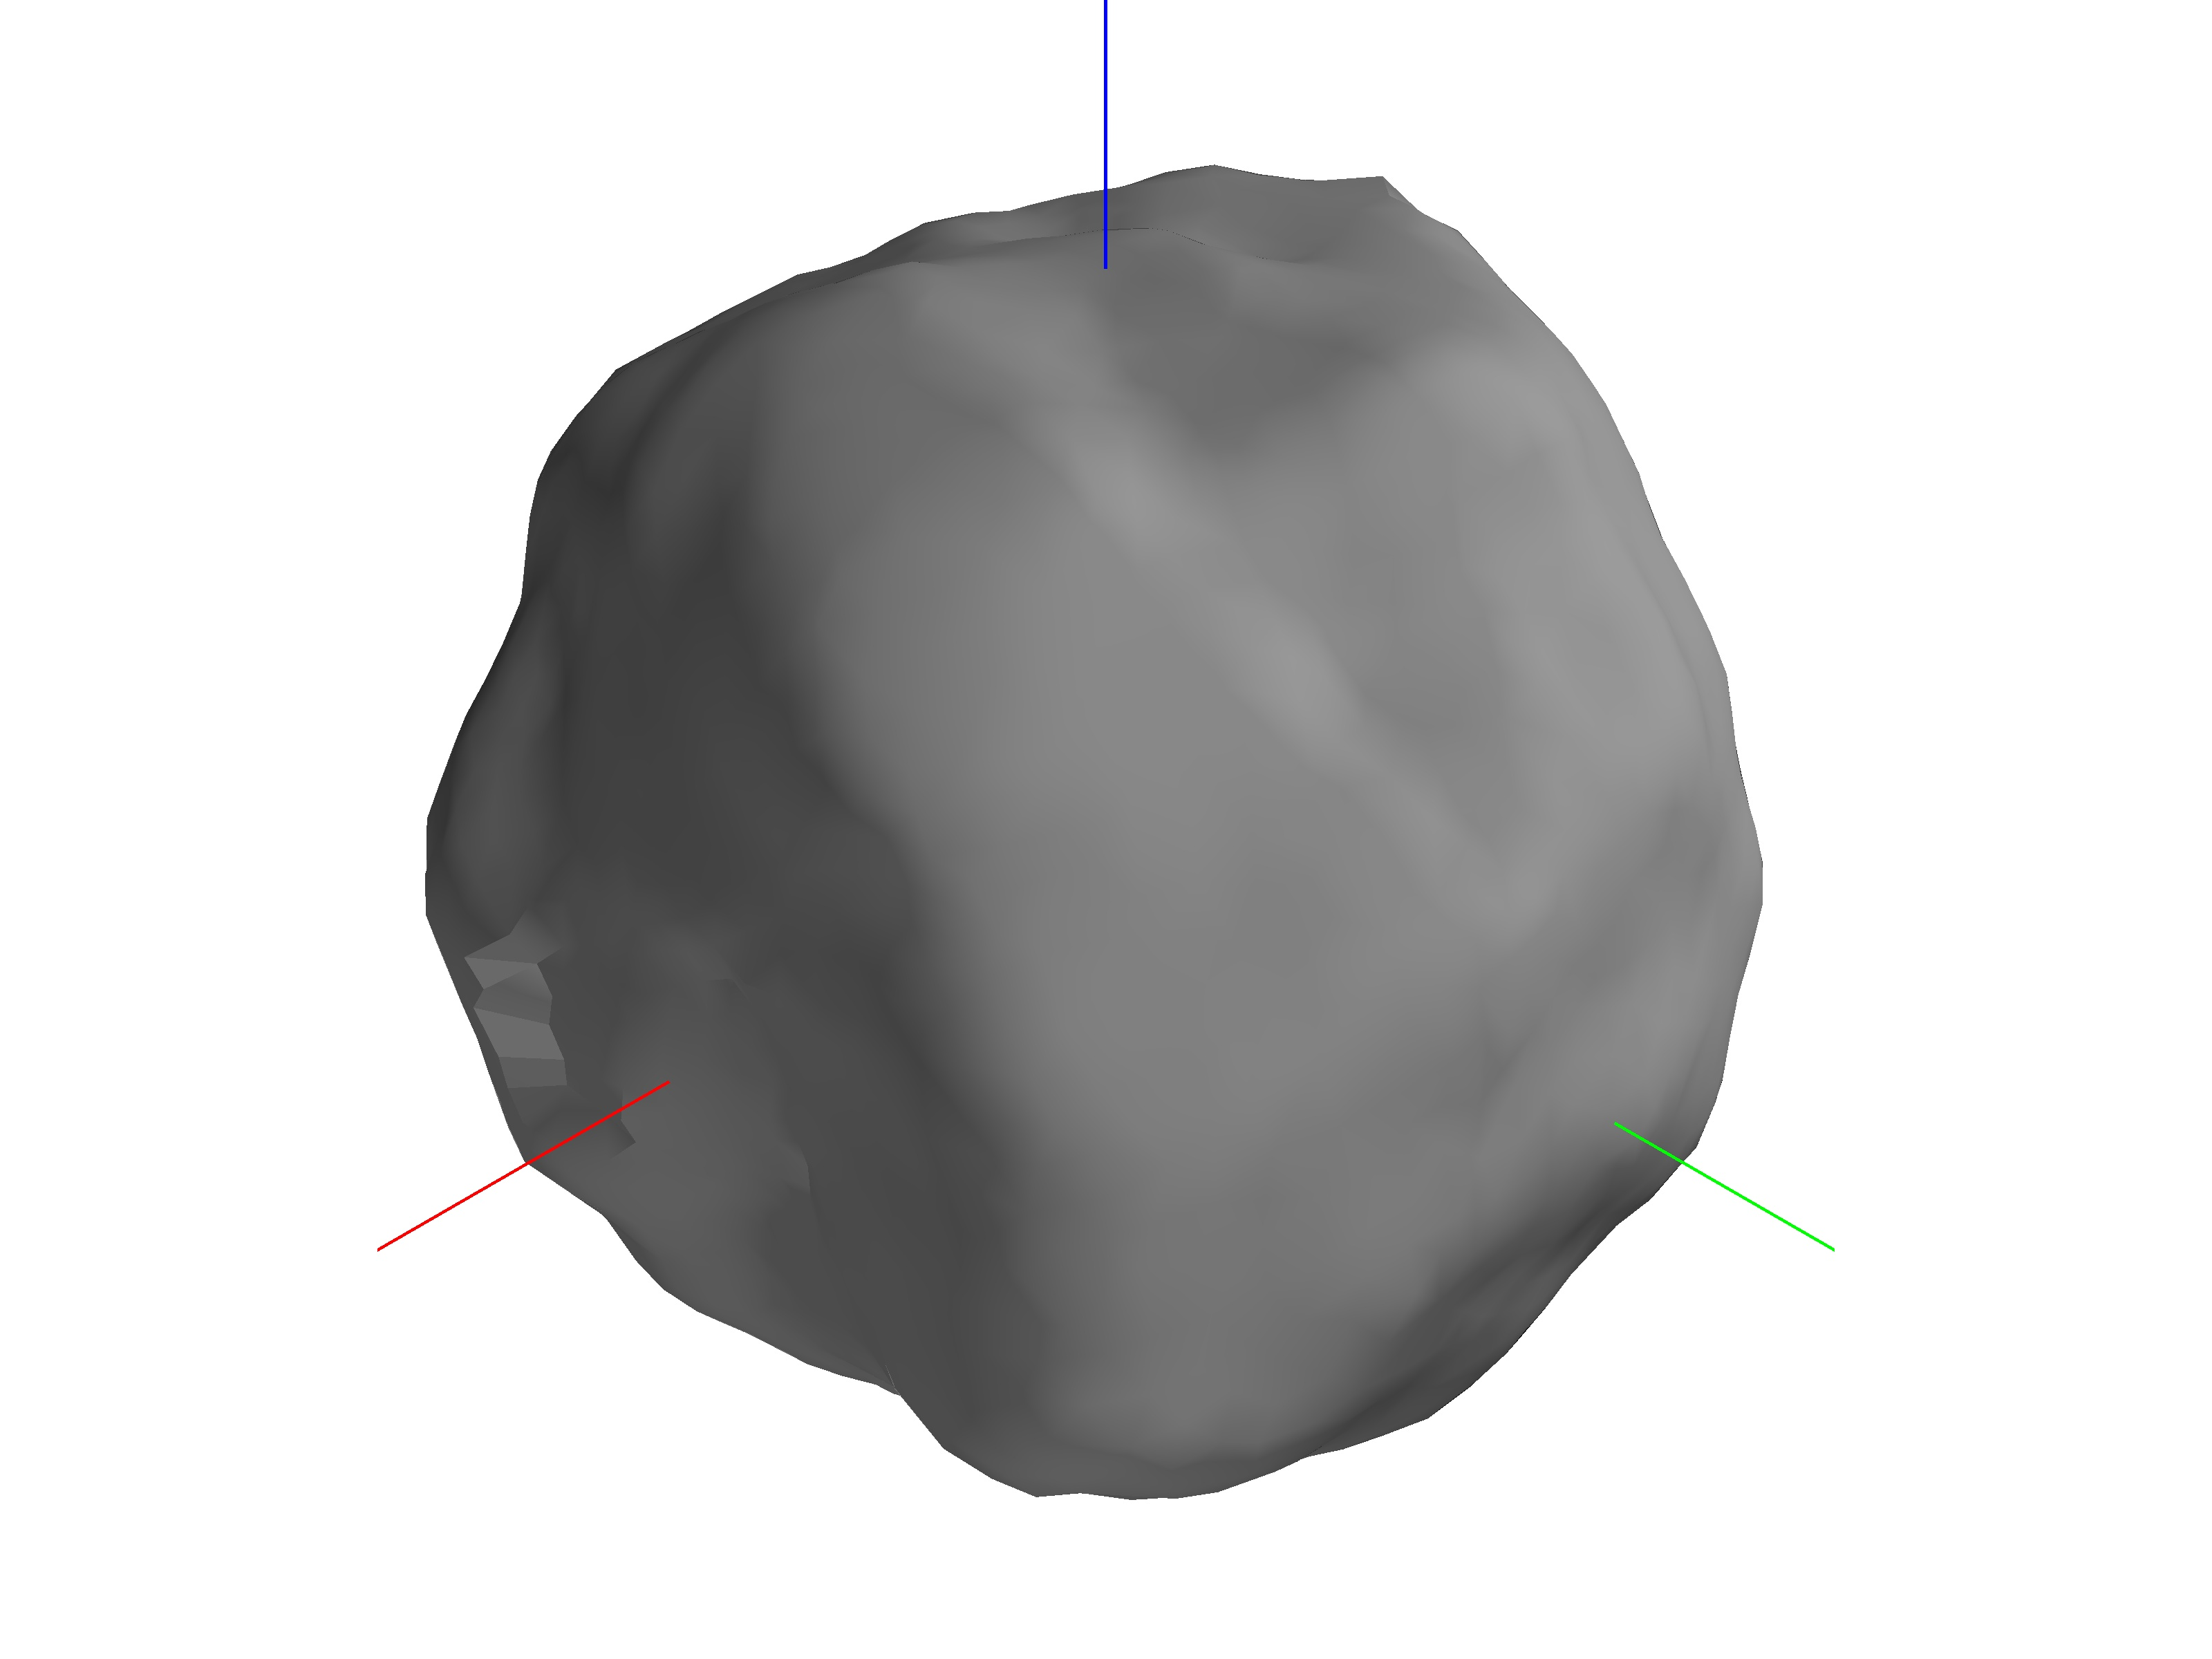
\includegraphics[width=0.5\textwidth]{figures/computational_geometry/dynamic_exploration/52760/partial_14998.jpg}}~
    \subcaptionbox{True Shape Model\label{fig:52760_truth}}{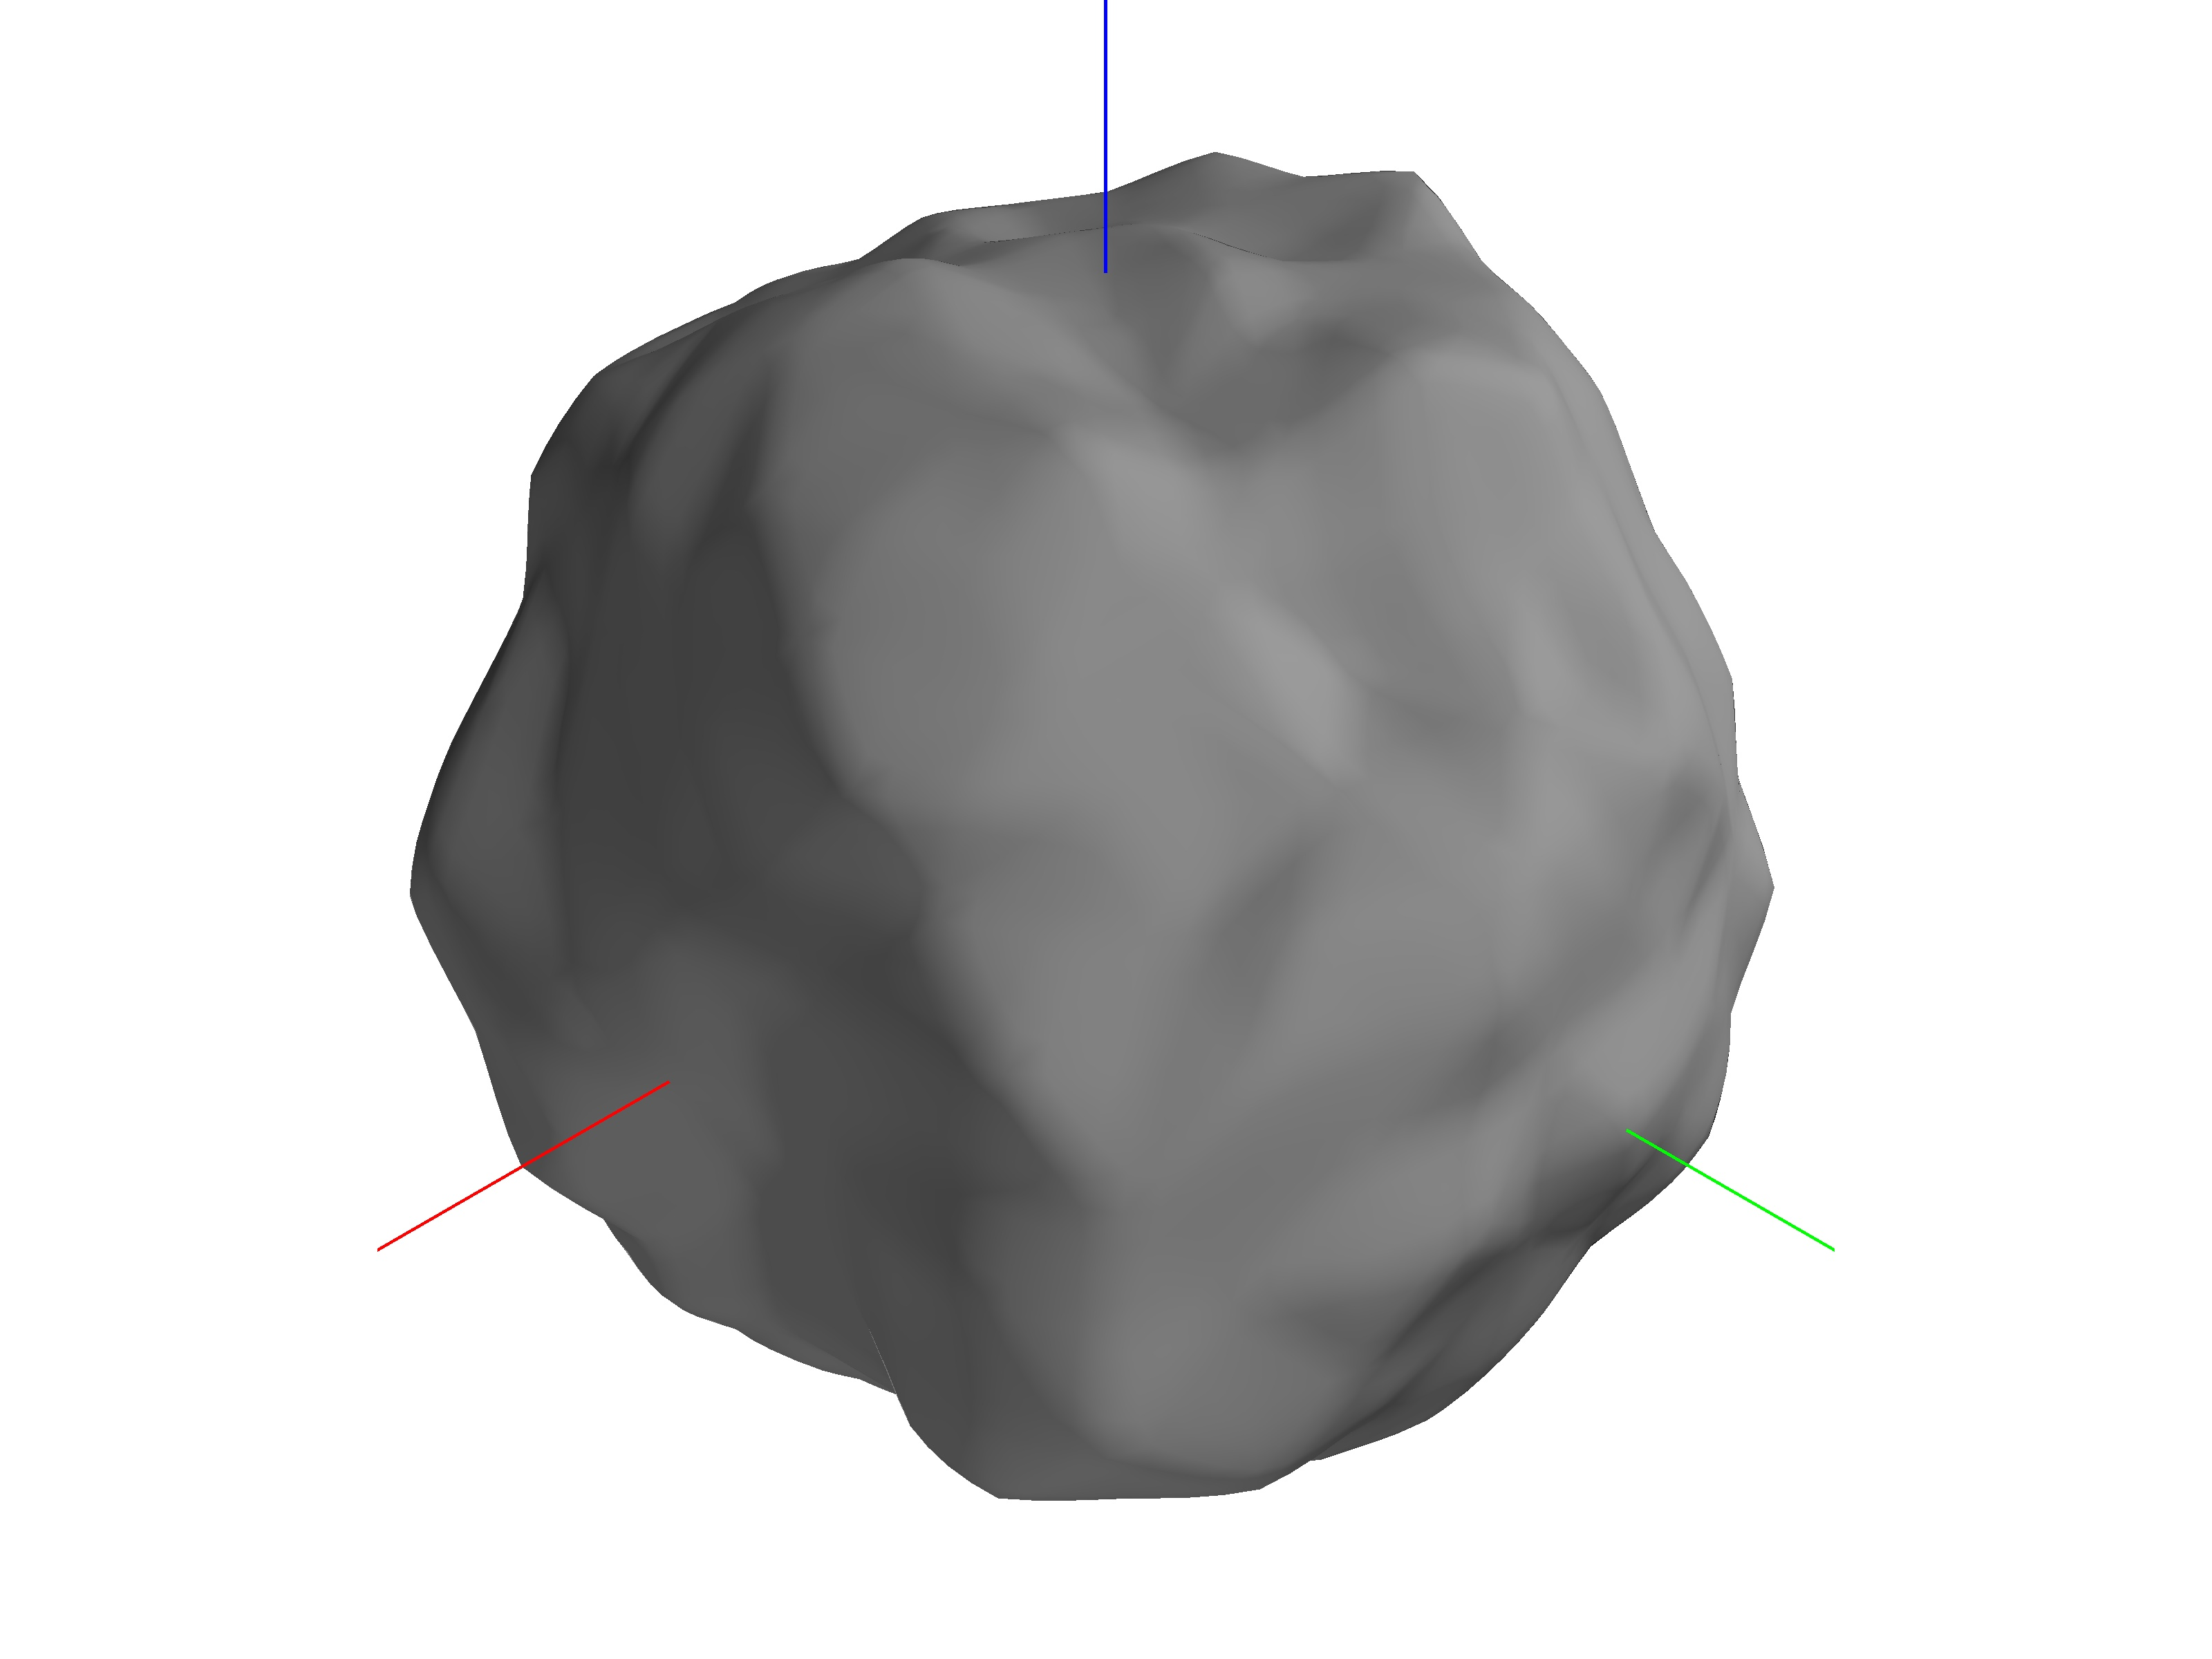
\includegraphics[width=0.5\textwidth]{figures/computational_geometry/mesh_update/52760/truth.jpg}}
    \caption[Asteroid 52760 Incremental Reconstruction]{Incremental Reconstruction of asteroid 52760~\label{fig:52760_reconstruction}}
\end{figure}

\begin{figure}[htbp]
    \centering
    \subcaptionbox{Initial Shape Estimate\label{fig:52760_partial_weights_0}}{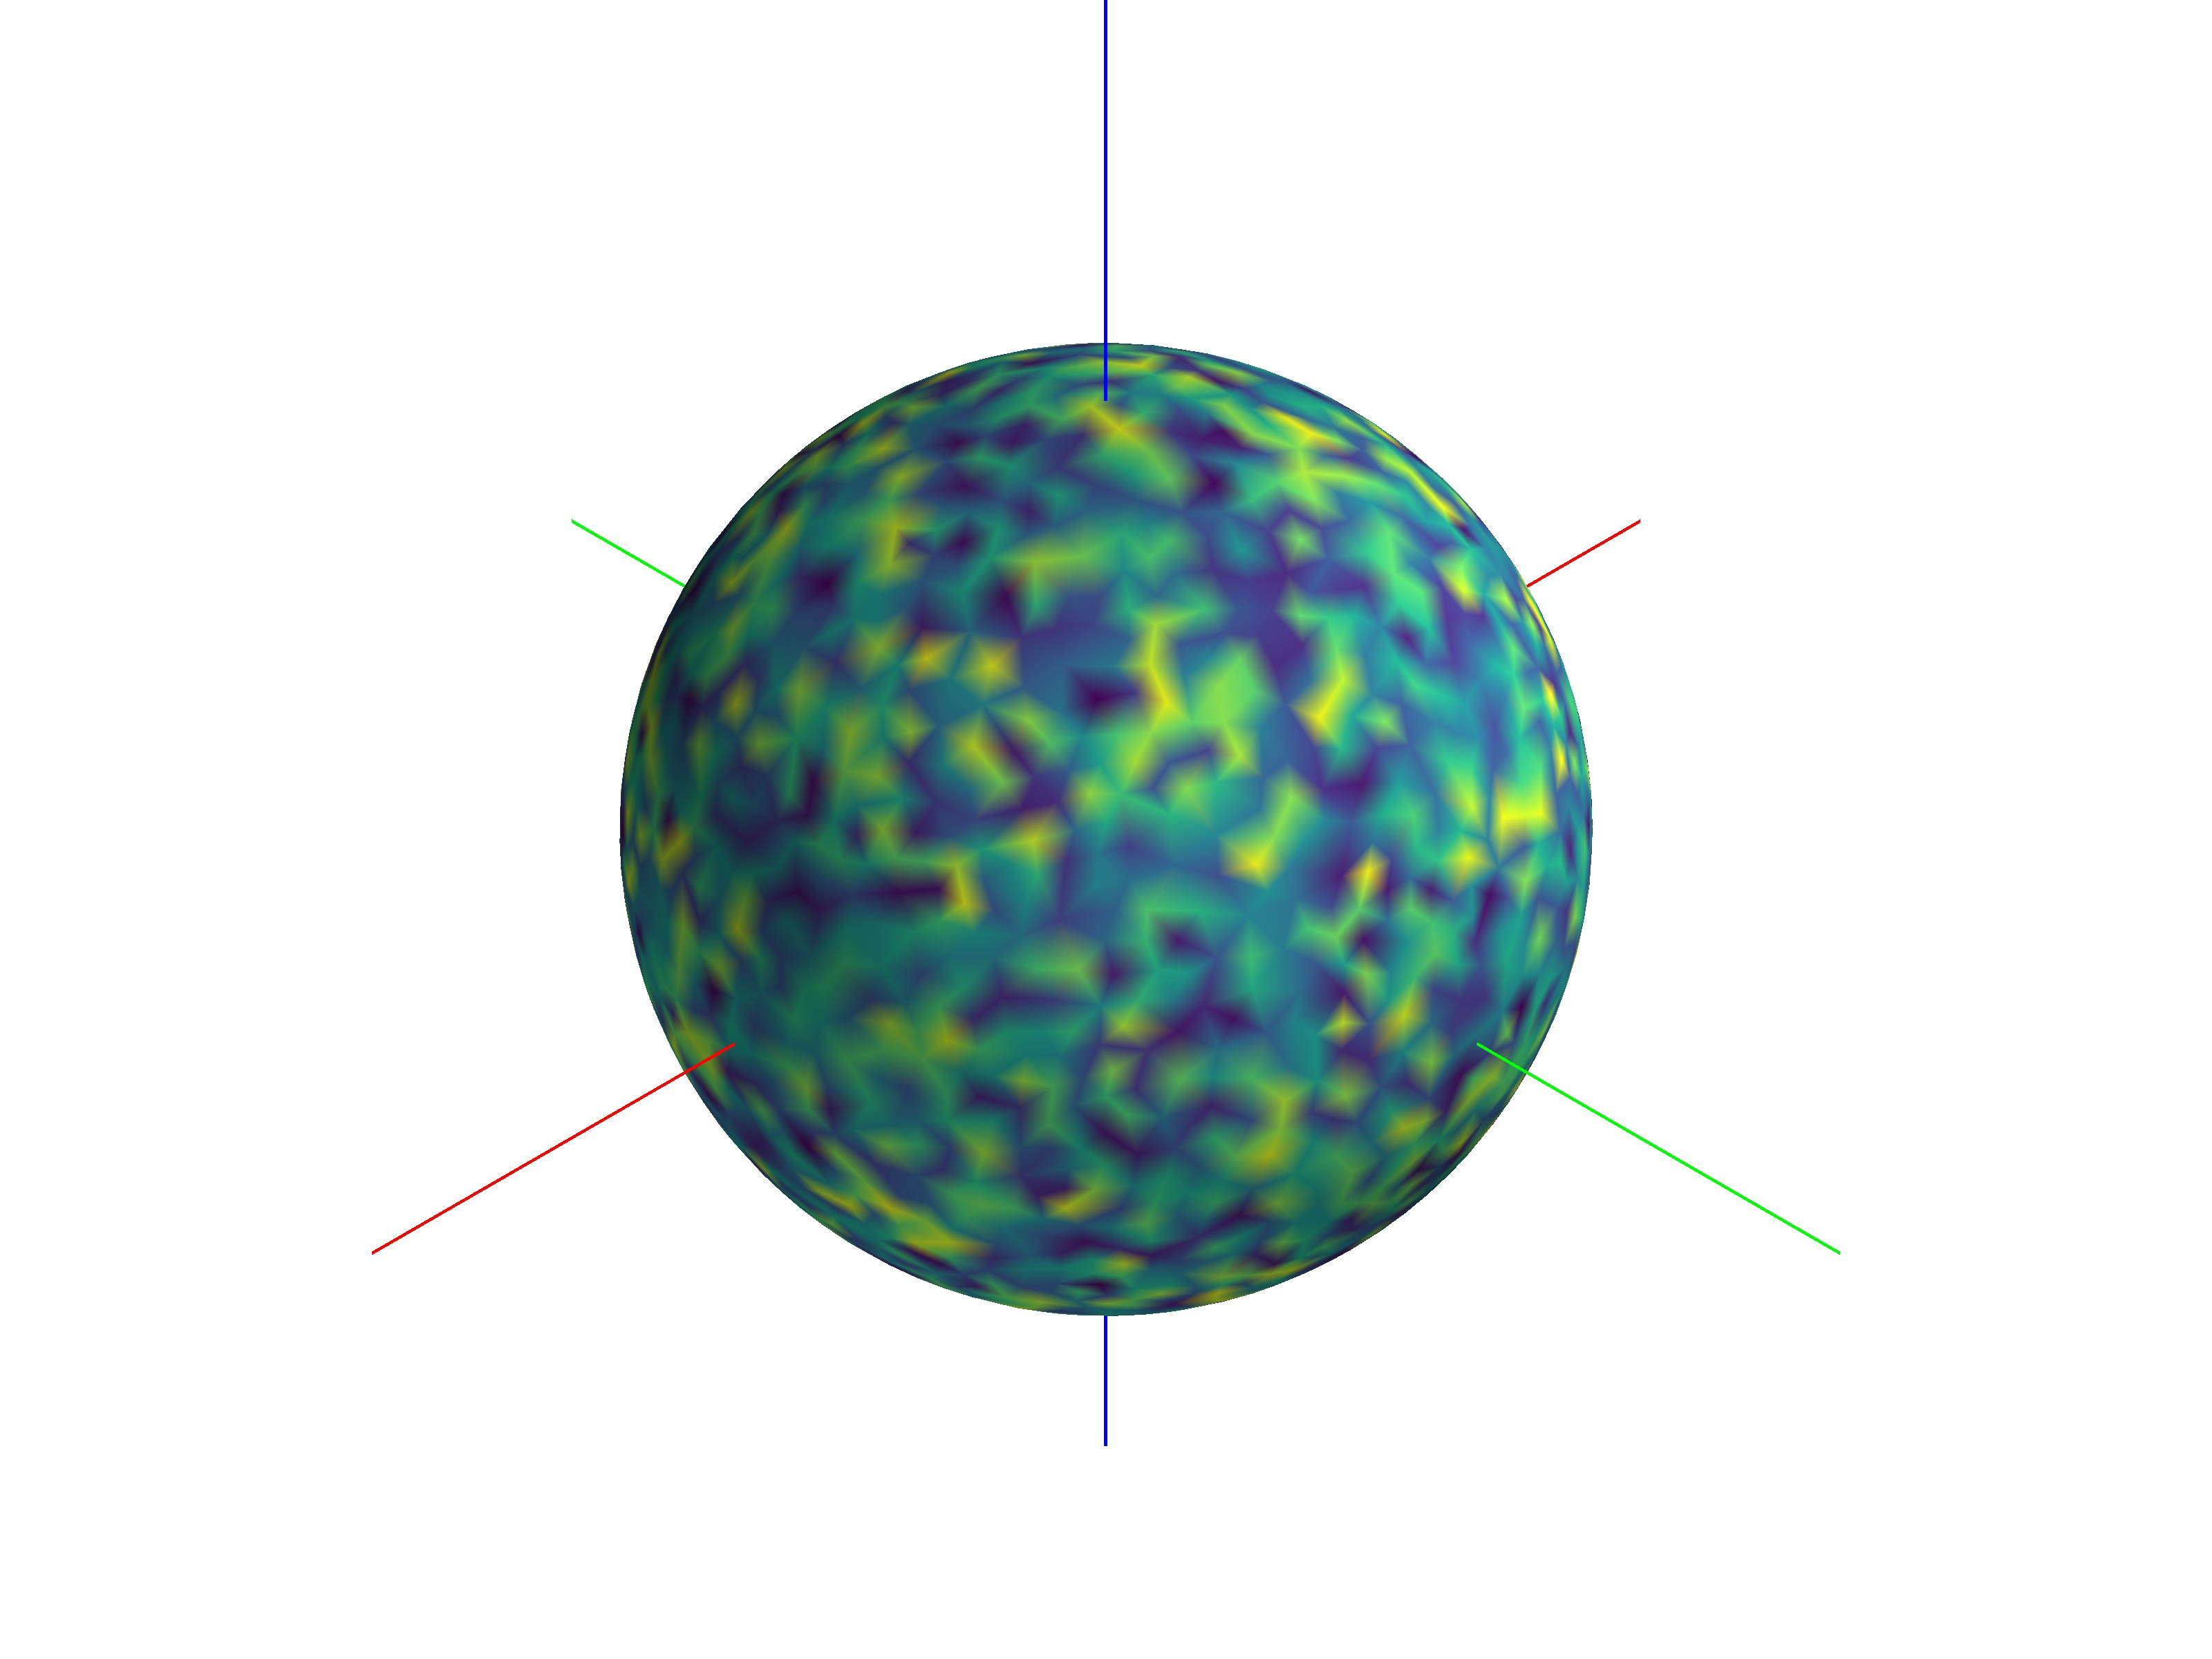
\includegraphics[height=0.5\textheight,width=0.5\textwidth,keepaspectratio]{figures/computational_geometry/dynamic_exploration/52760/partial_weights_1.jpg}}~
    \subcaptionbox{\SI{25}{\percent} of measurements added\label{fig:52760_partial_weights_25}}{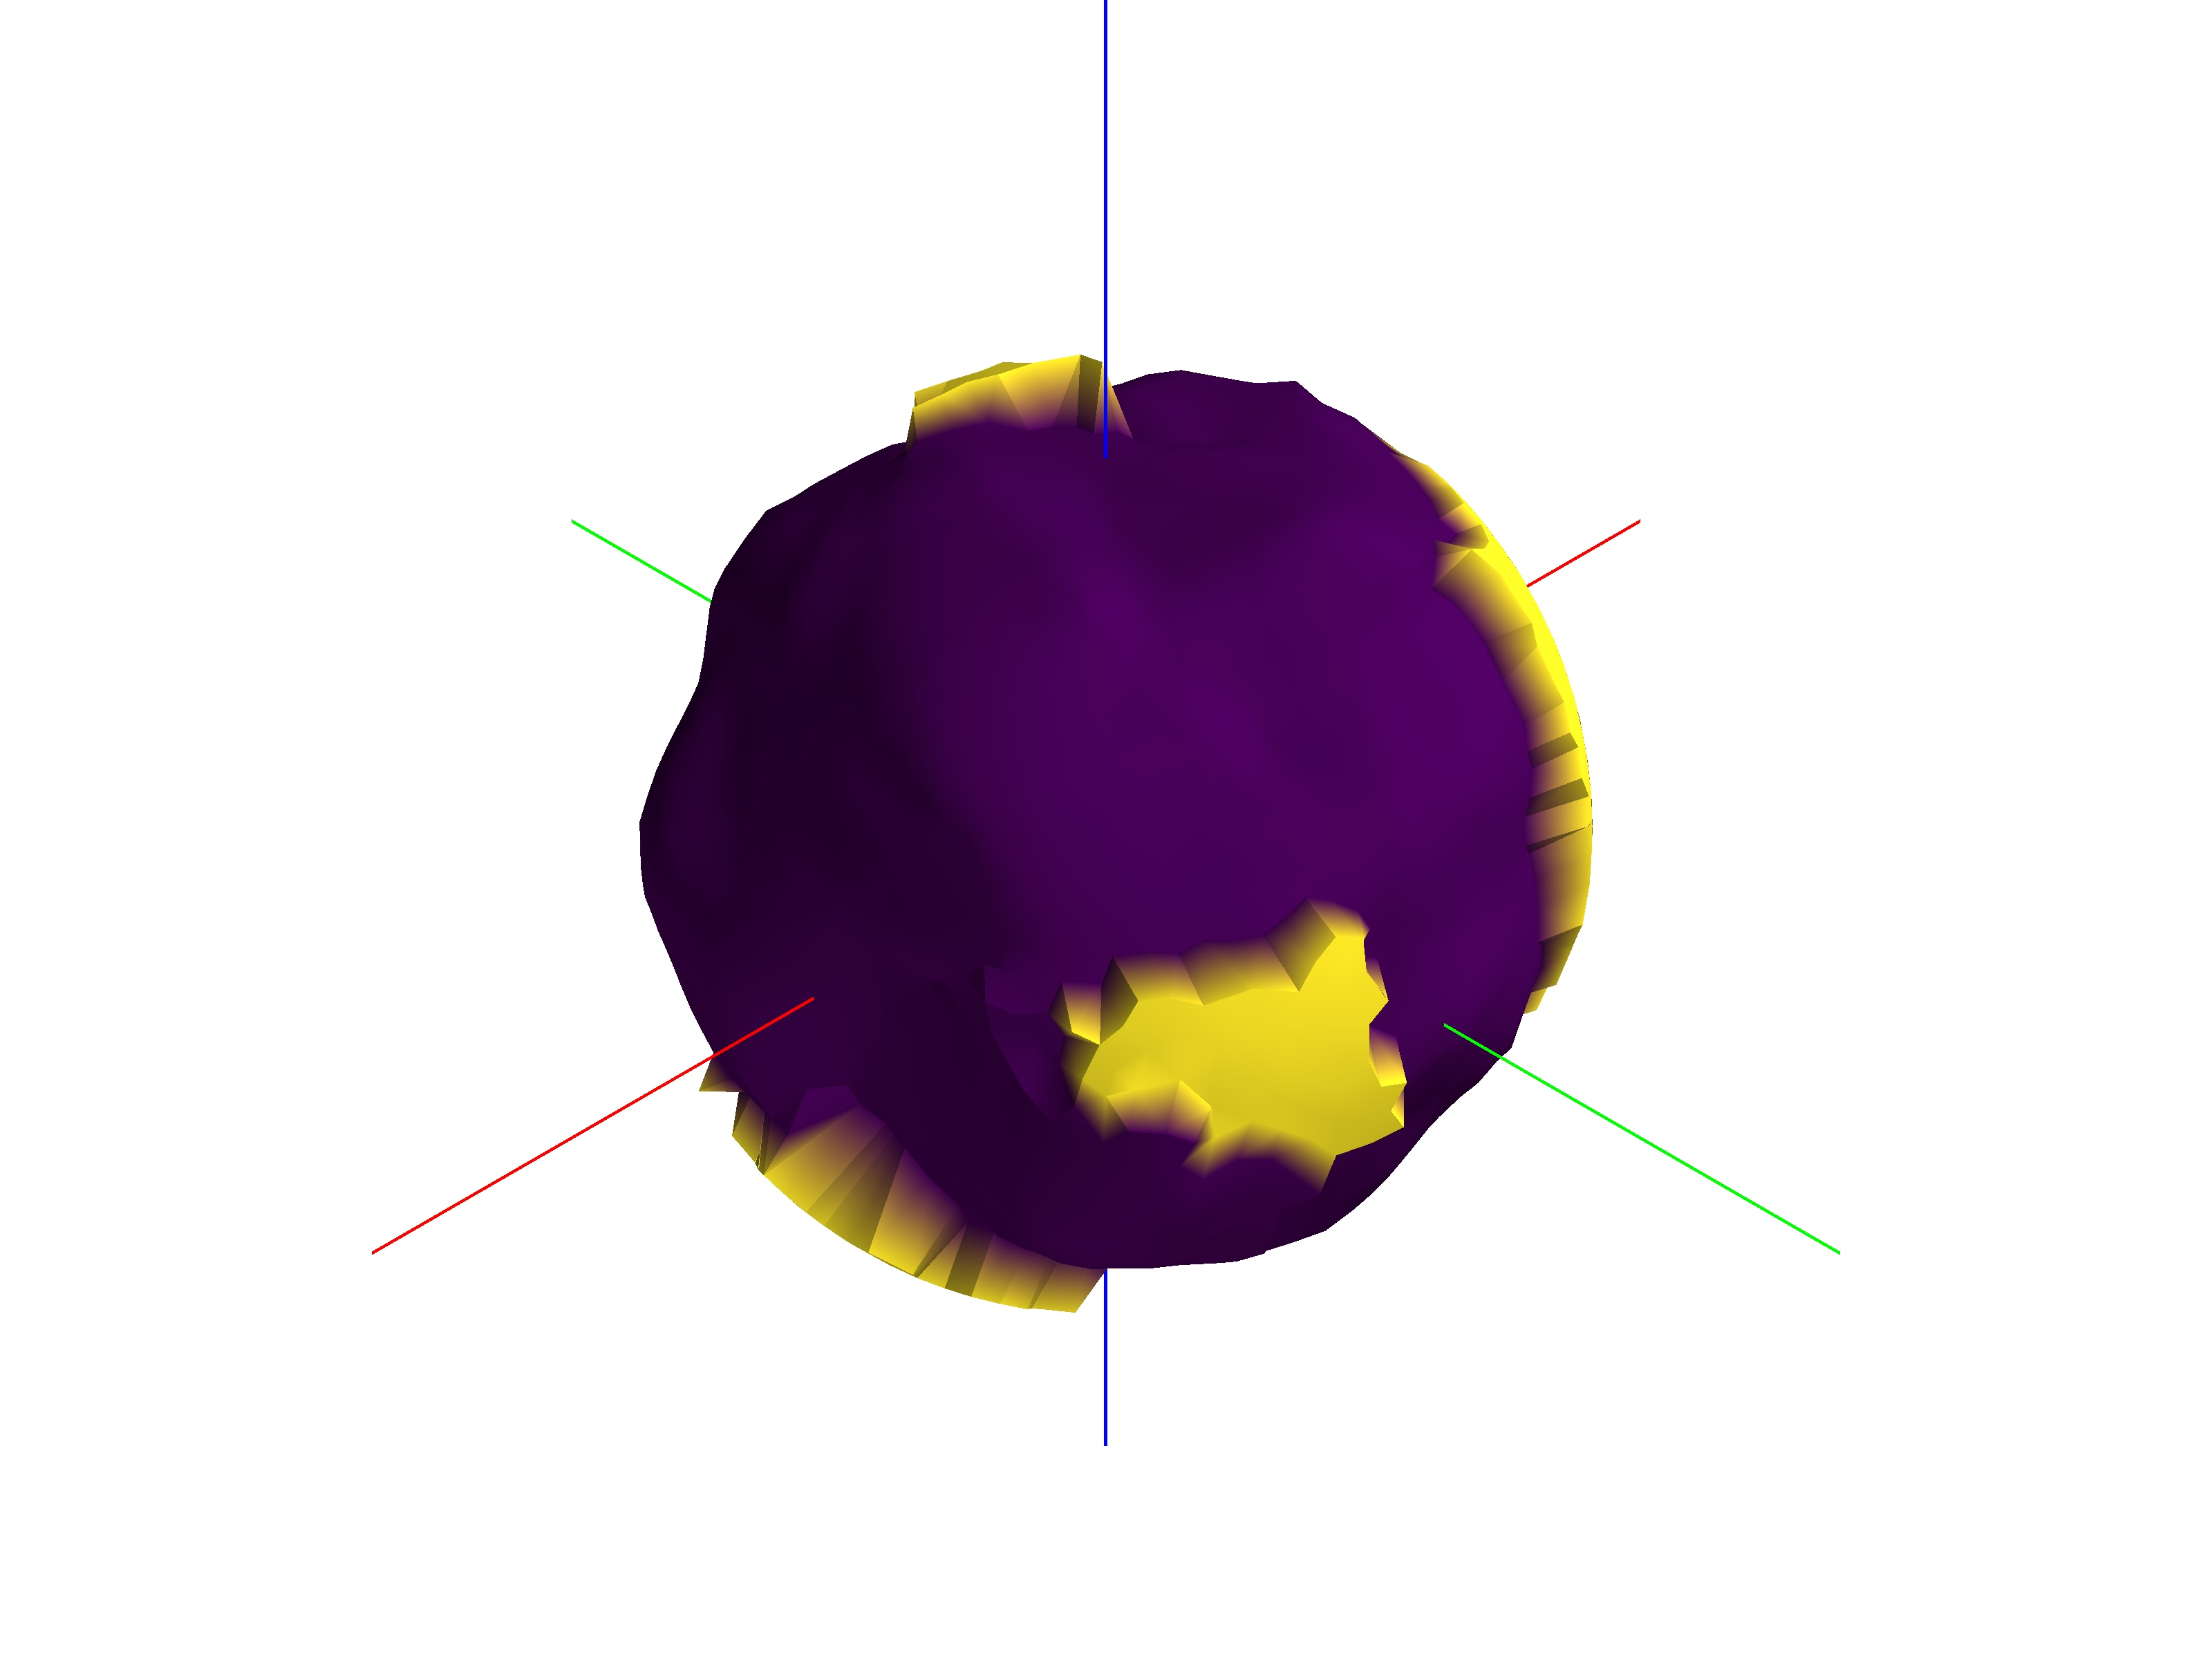
\includegraphics[width=0.5\textwidth]{figures/computational_geometry/dynamic_exploration/52760/partial_weights_3749.jpg}}

    \subcaptionbox{\SI{50}{\percent} of measurments added\label{fig:52760_partial_weights_50}}{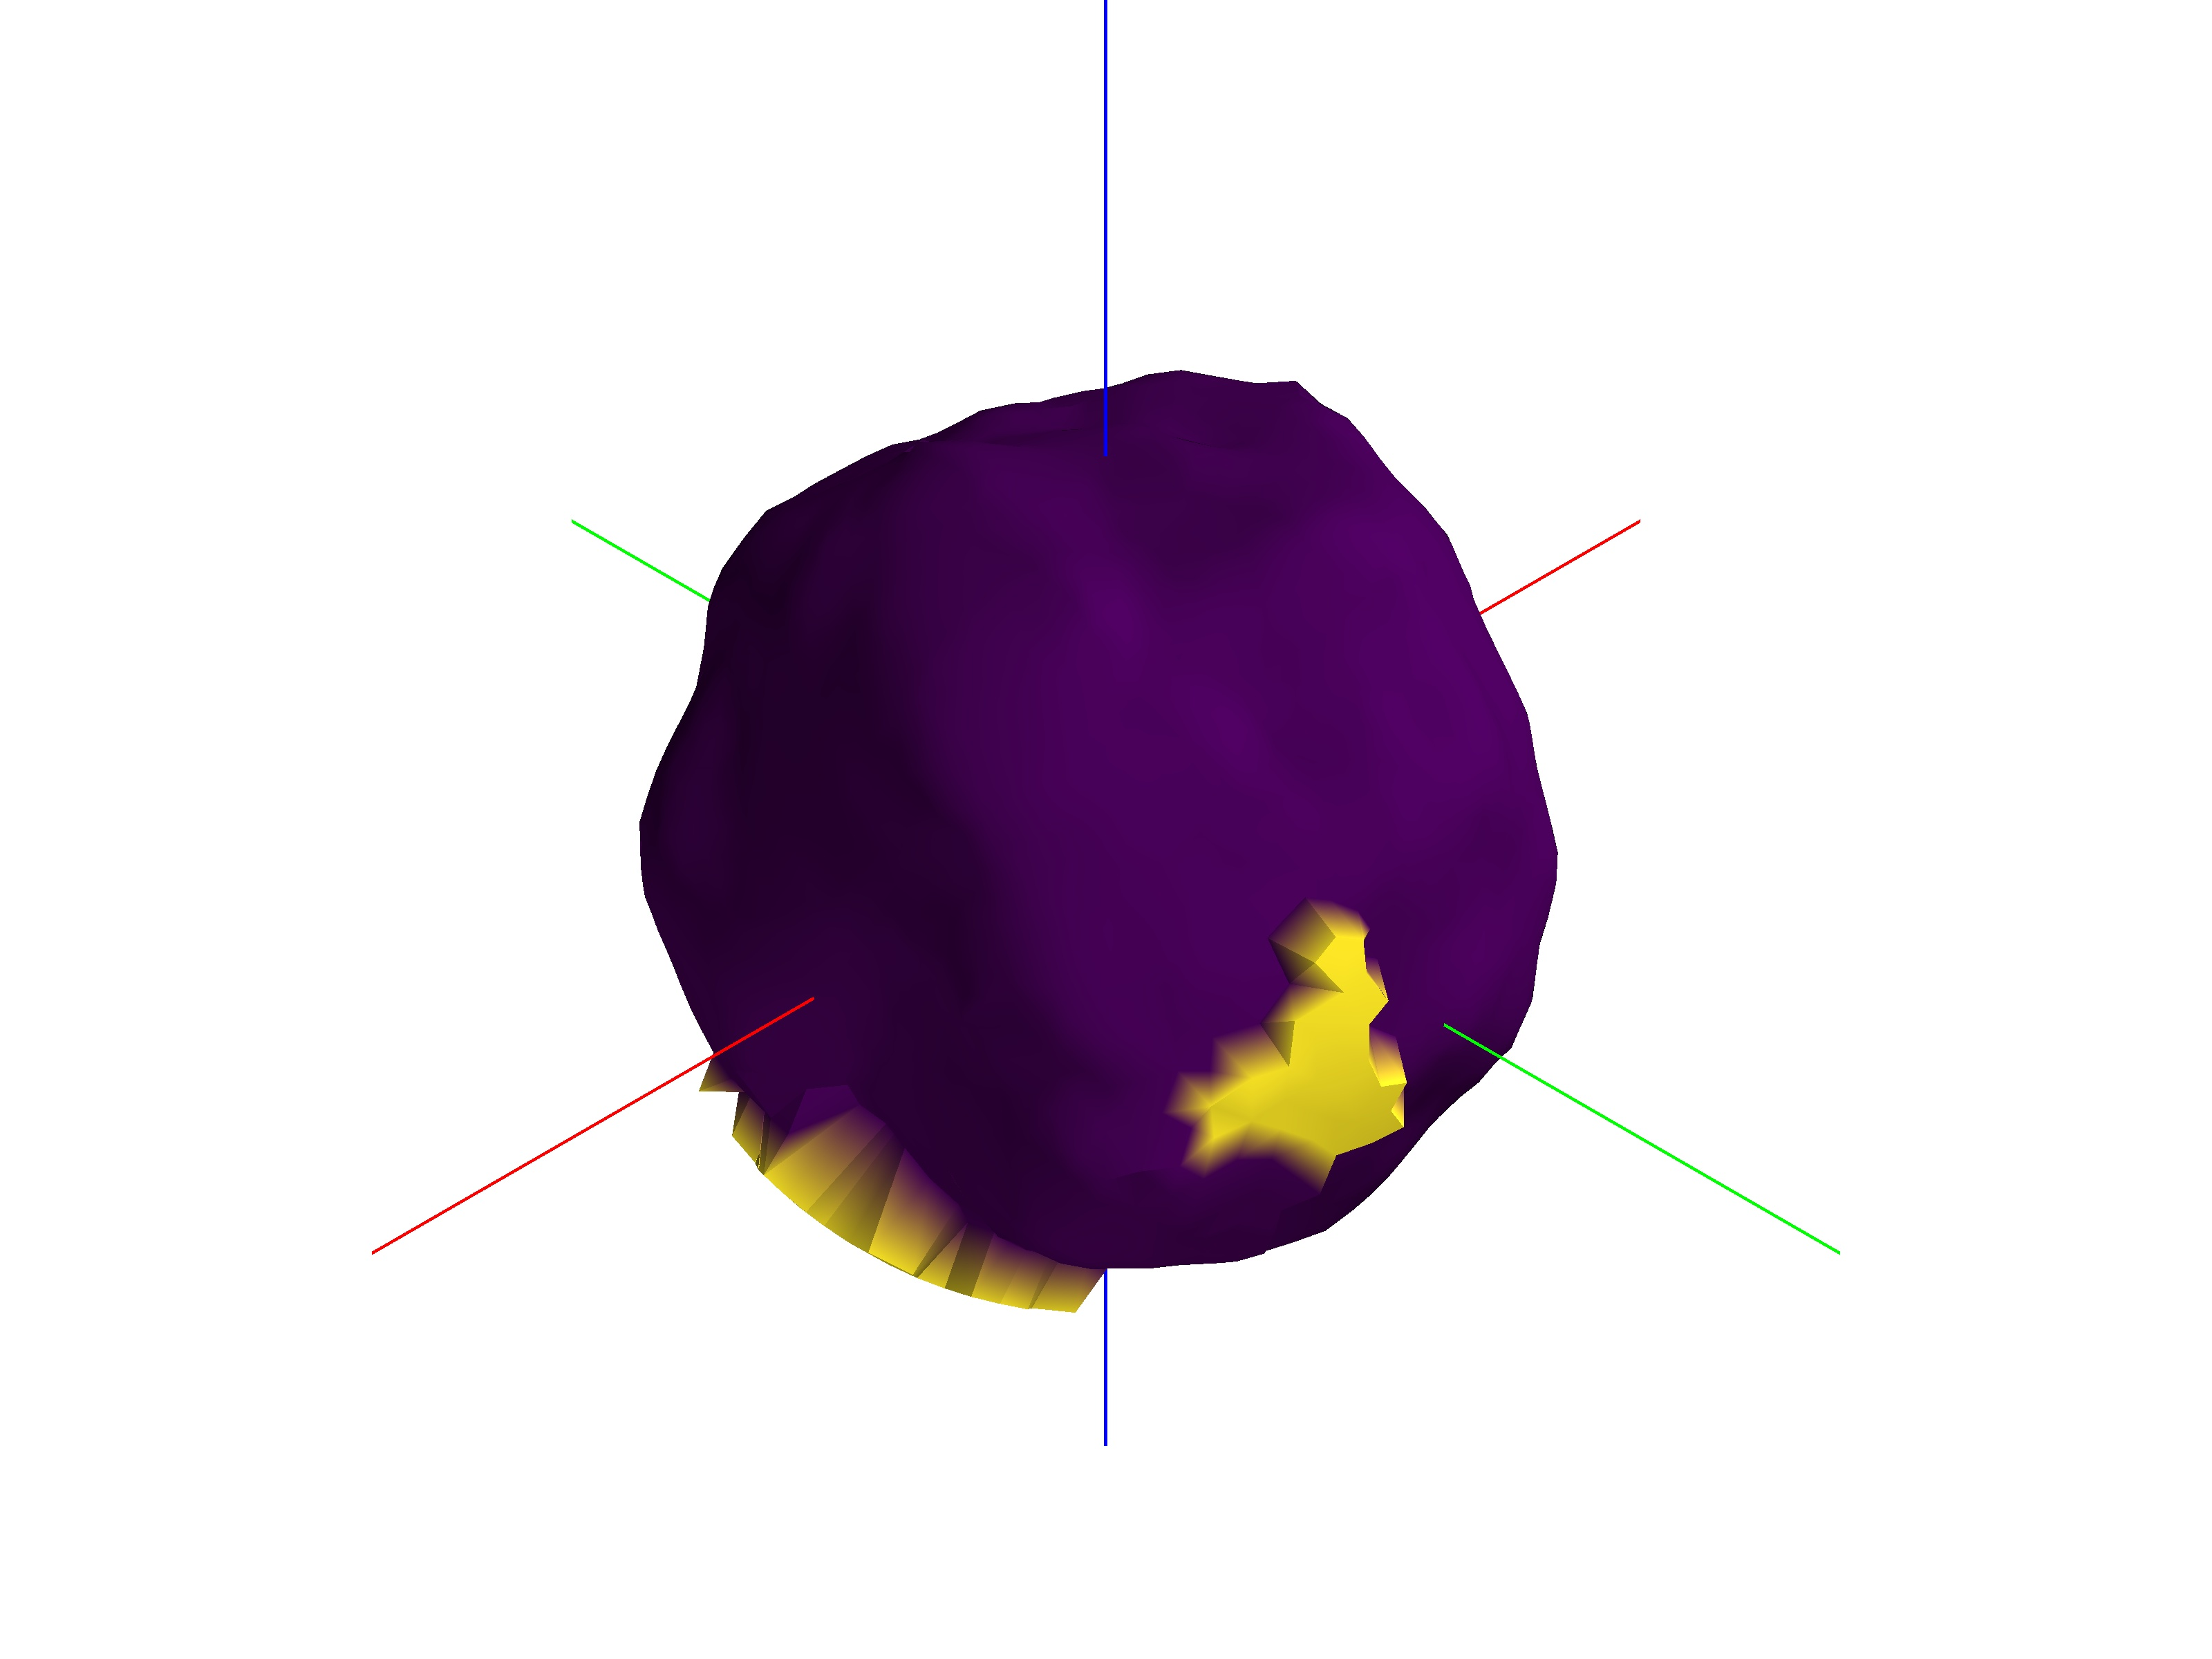
\includegraphics[width=0.5\textwidth]{figures/computational_geometry/dynamic_exploration/52760/partial_weights_7499.jpg}}~
    \subcaptionbox{\SI{75}{\percent} of measurements added\label{fig:52760_partial_weights_75}}{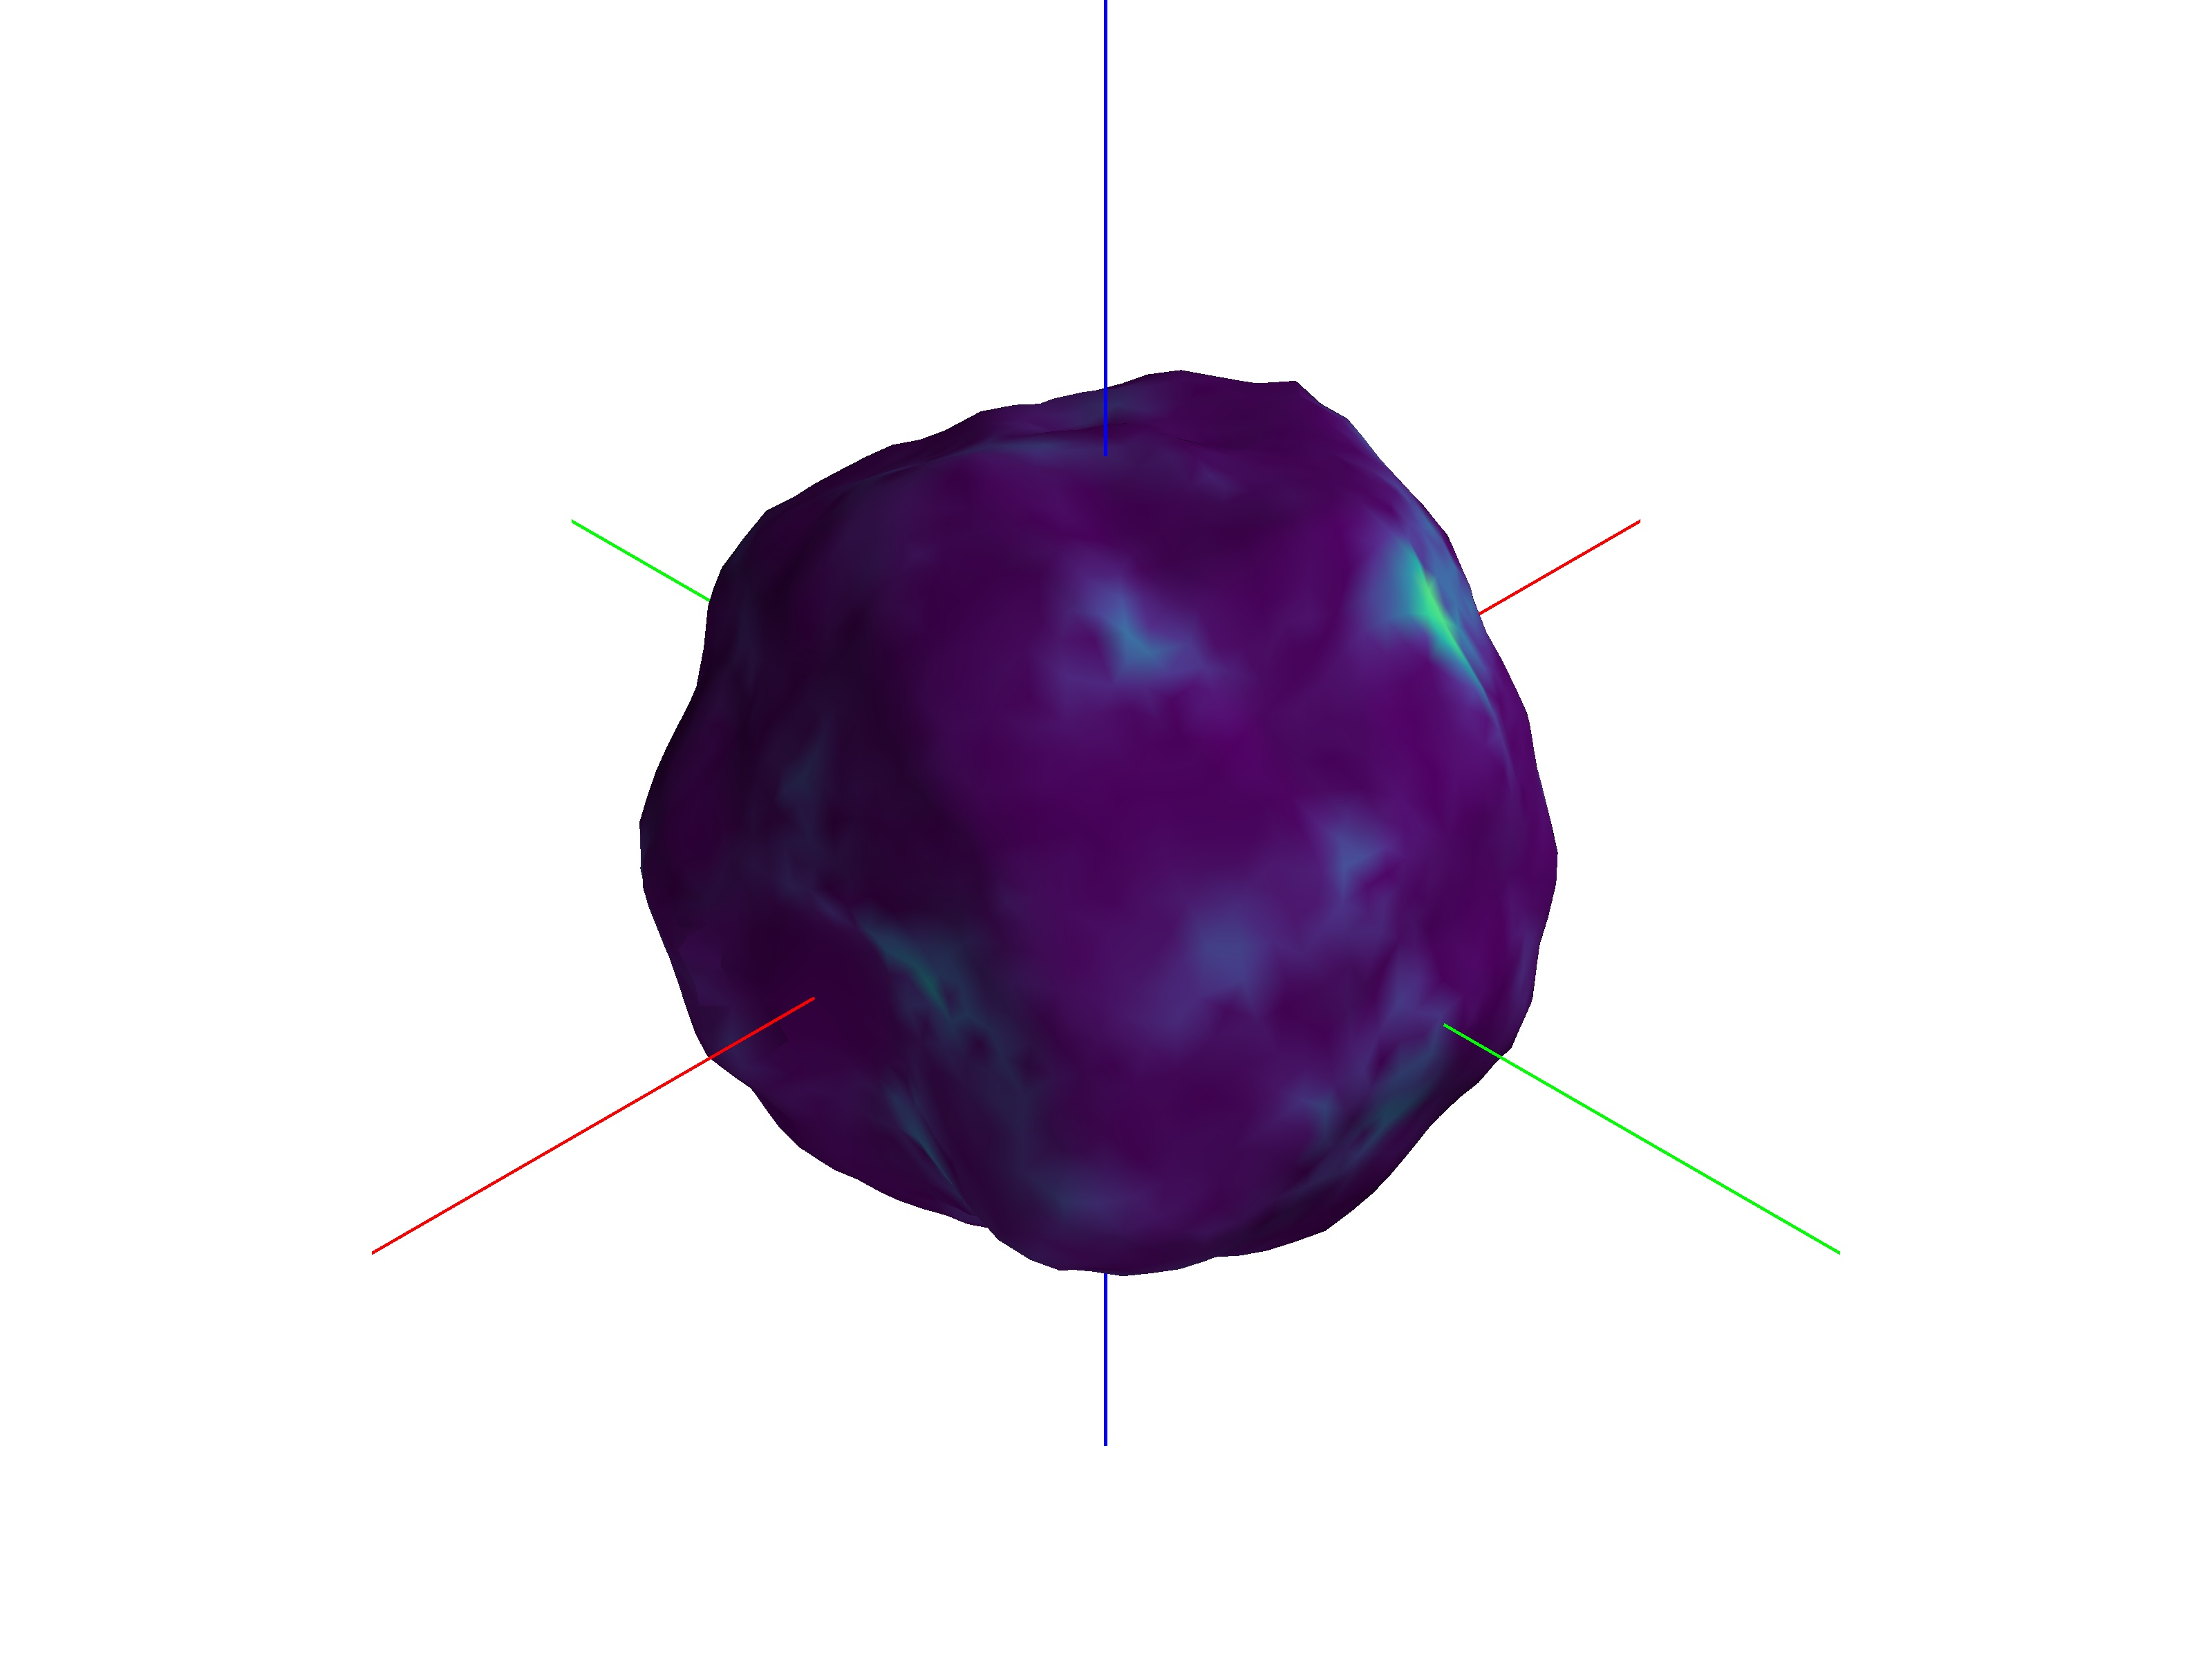
\includegraphics[width=0.5\textwidth]{figures/computational_geometry/dynamic_exploration/52760/partial_weights_11249.jpg}}

    \subcaptionbox{\SI{100}{\percent} of measurements added\label{fig:52760_partial_weights_100}}{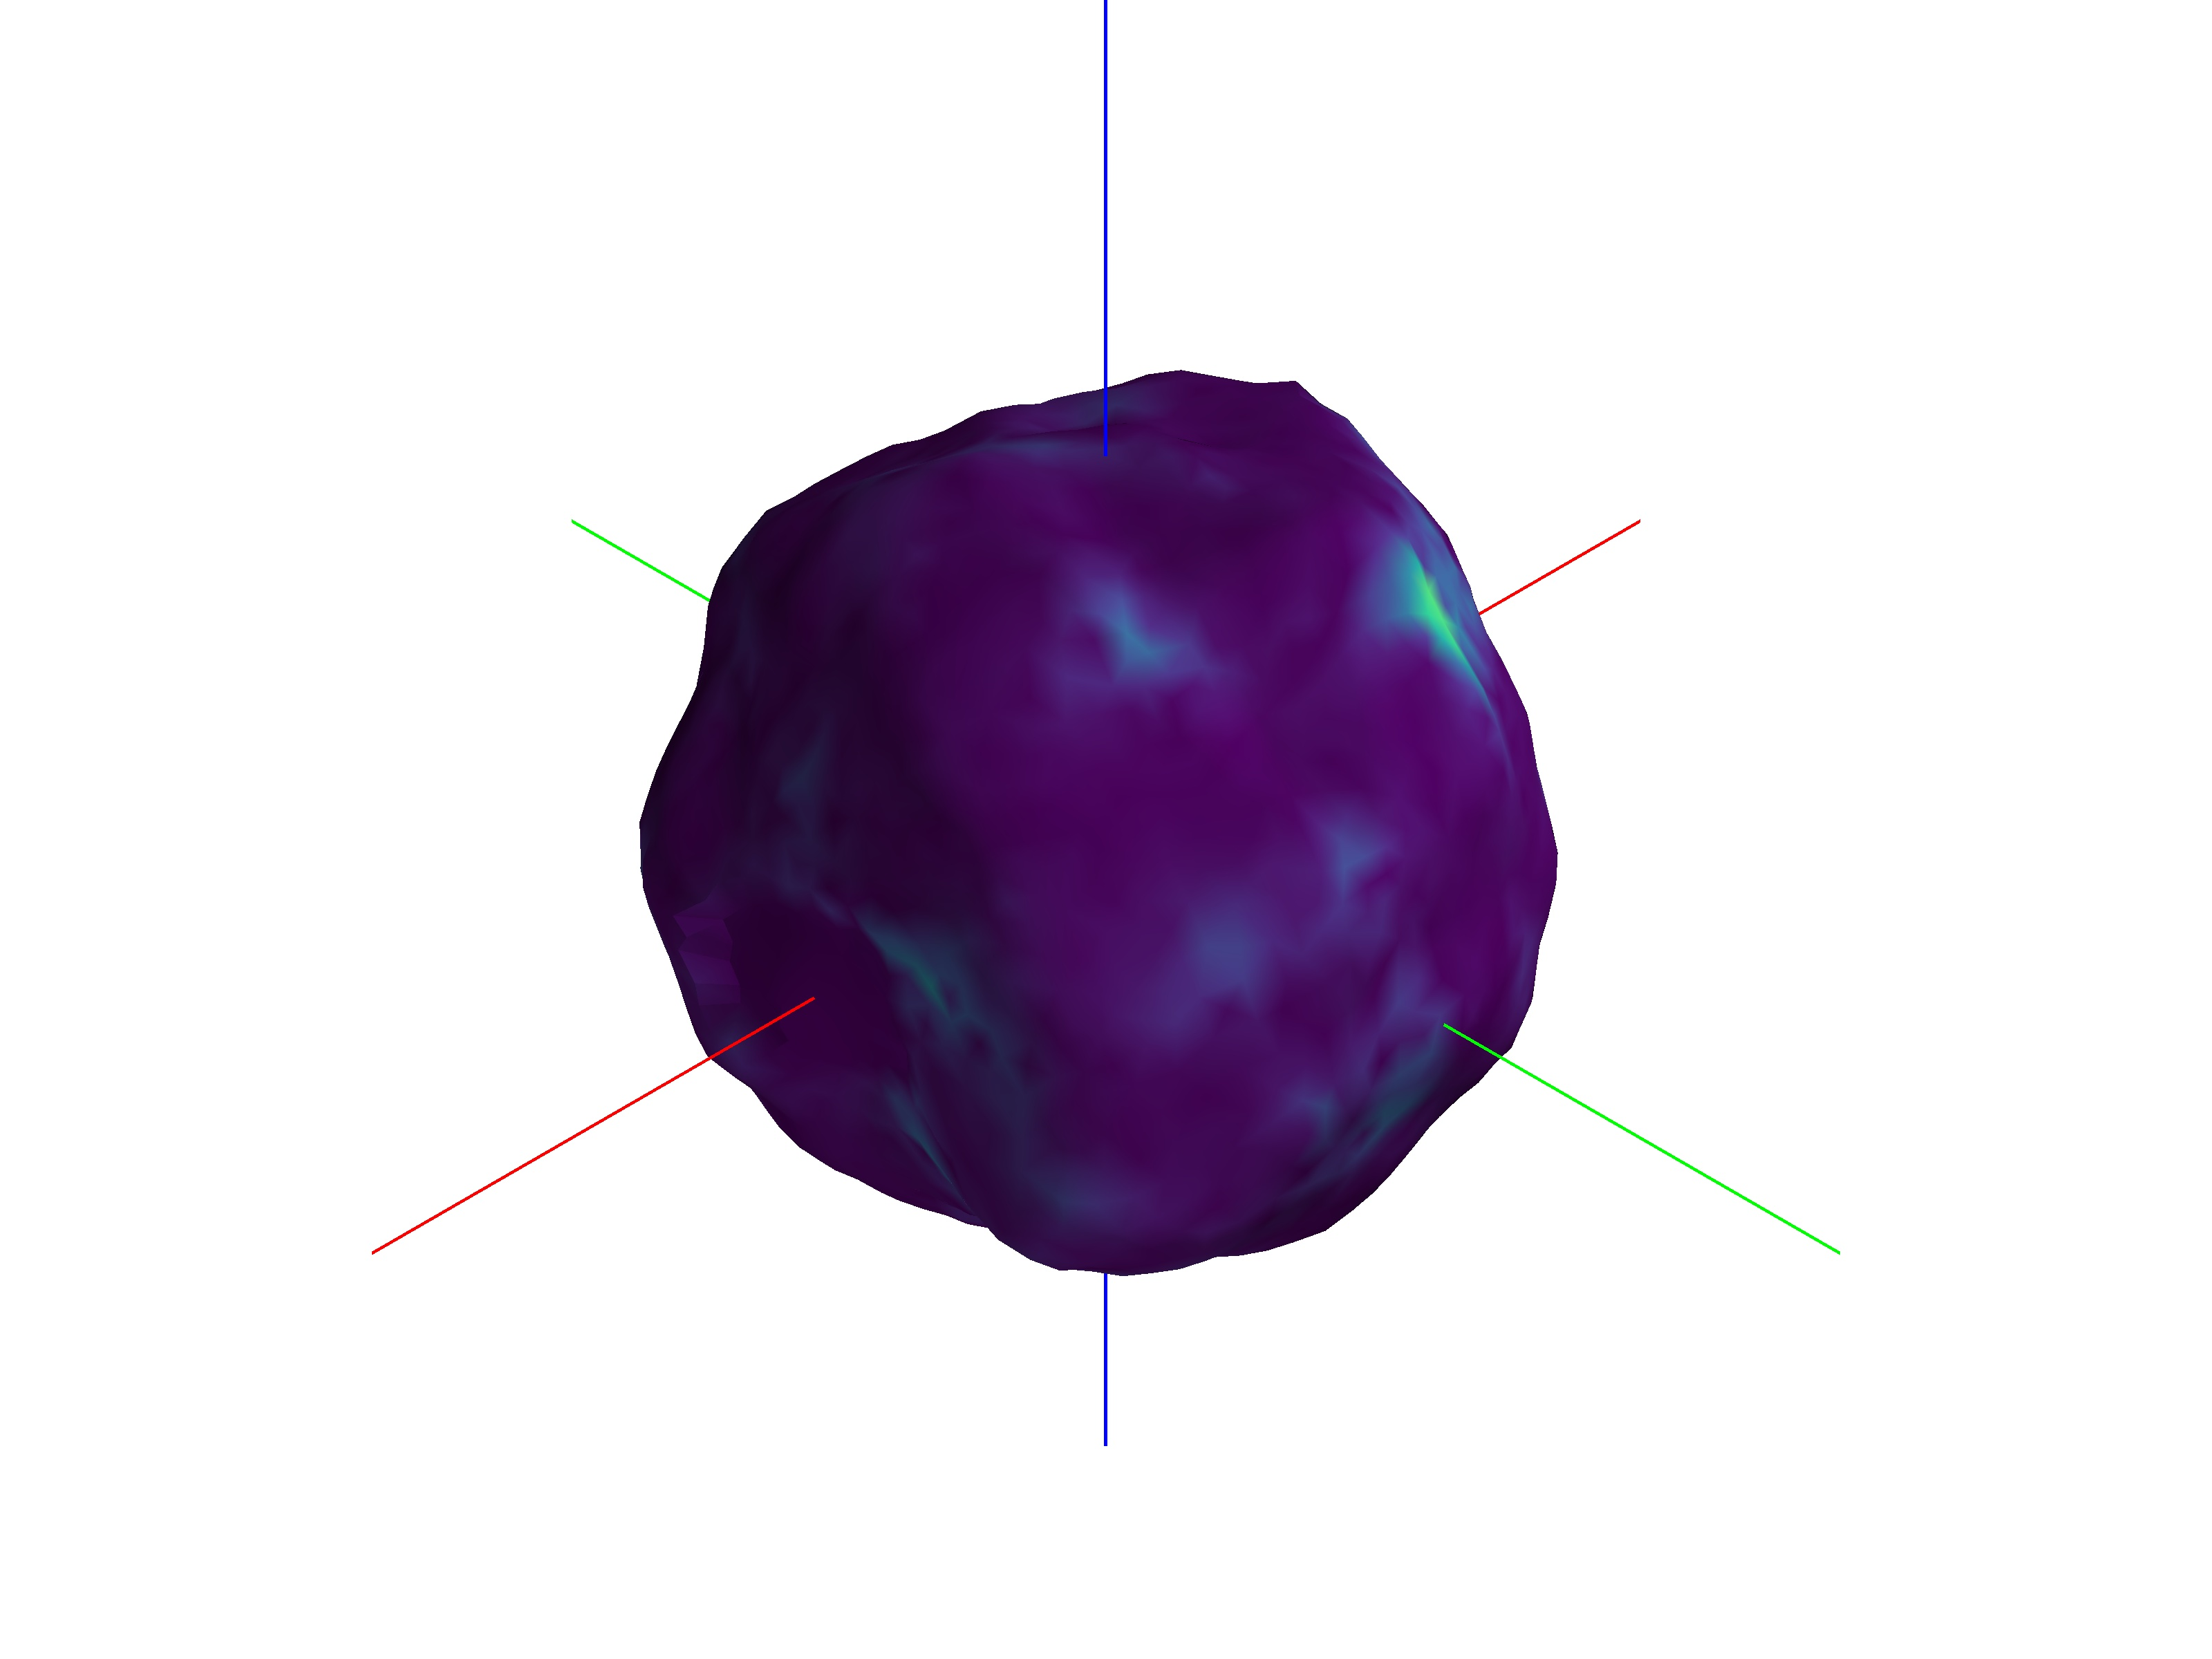
\includegraphics[width=0.5\textwidth]{figures/computational_geometry/dynamic_exploration/52760/partial_weights_14998.jpg}}~
    \subcaptionbox{True Shape Model\label{fig:52760_weights_truth}}{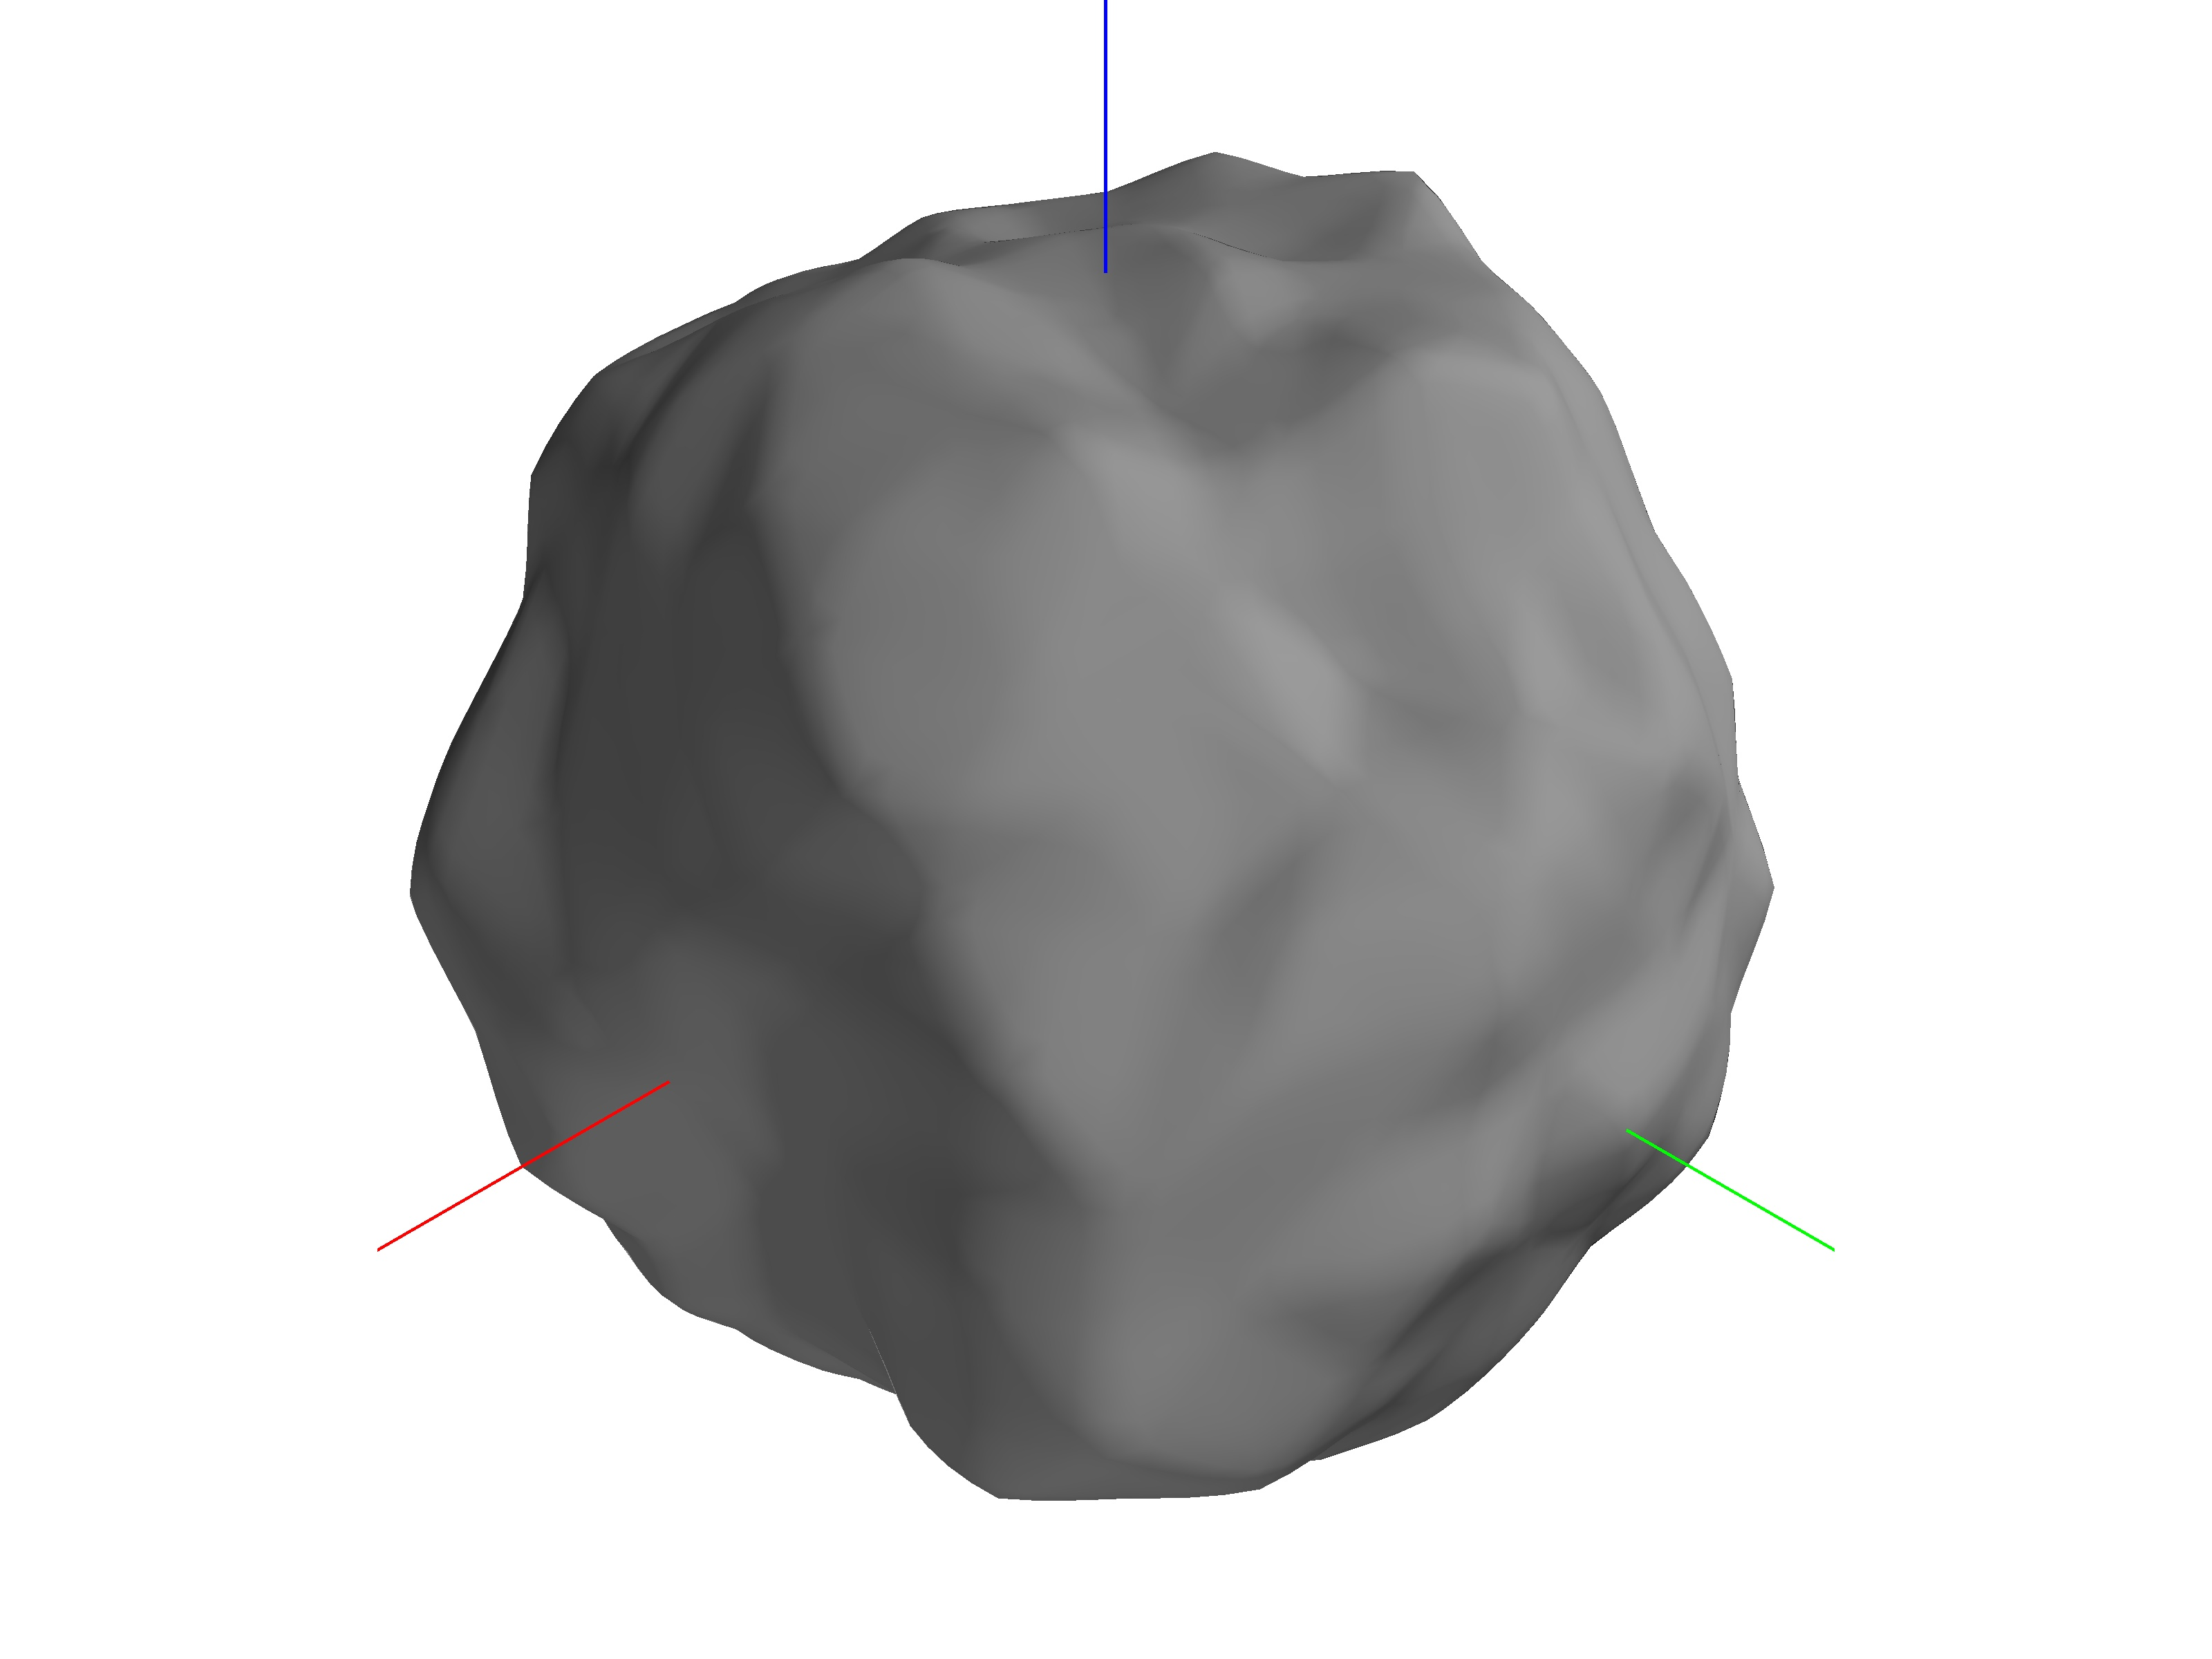
\includegraphics[width=0.5\textwidth]{figures/computational_geometry/mesh_update/52760/truth.jpg}}
    \caption[Asteroid 52760 Shape Reconstruction with Uncertainty]{Incremental Reconstruction of asteroid 52760. The images colored according to the shape uncertainty. Areas of high uncertainty are in yellow while ares of low uncertainty are in purple.~\label{fig:52760_weights_reconstruction}}
\end{figure}
\Cref{fig:52760_metrics} shows the total normalized uncertainty and percent error for the volume estimate. 
The plots show that the reconstruction  converges to an accurate shape estimate after approximately \SI{8000}{\second}.
\begin{figure}[htbp]
    \centering
    \subcaptionbox{Normalized Uncertainty\label{fig:52760_uncertainty}}{\includegraphics[width=0.5\textwidth,height=0.31\textwidth]{tikz/52760_uncertainty.tikz}}~
    \subcaptionbox{Volume Percent Error\label{fig:52760_volume}}{\includegraphics[width=0.5\textwidth,height=0.31\textwidth]{tikz/52760_volume.tikz}}
    \caption{Normalized uncertainty and volume percent error for 52760\label{fig:52760_metrics}}
\end{figure}

\paragraph{Asteroid 4769 Castalia Reconstruction}
Asteroic 4769 Castalia is a small near Earth asteroid of the Apollo group.
In addition, it is classified as a potentially hazardous object with a closed approach distance of less than \SI{0.05}{\astronomicalunit}.
Castalia was discoved in \num{1989} and is the first asteroid to be modeled using radar imagery~\cite{hudson1994}.
Castalia is composed of two distinct lobes suggesting that it is a contact binary of two smaller objects held together by their mutal gravity.
\Cref{fig:castalia_reconstruction,fig:castalia_weights_reconstruction} show the shape reconstruction at several discrete points during the simulation.
In addition~\cref{fig:castalia_weights_reconstruction} displays the vertex uncertainty \( w_i \) as a colormap on the surface. 
Areas of high uncertainty are denoted in yellow while areas of low uncertainty are in purple/blue.
Within \SI{50}{\percent} of the simulation span the spacecraft is able to achieve an accurate estimate of the true shape of Castalia.
\begin{figure}[htbp]
    \centering
    \subcaptionbox{Initial Shape Estimate\label{fig:castalia_partial_0}}{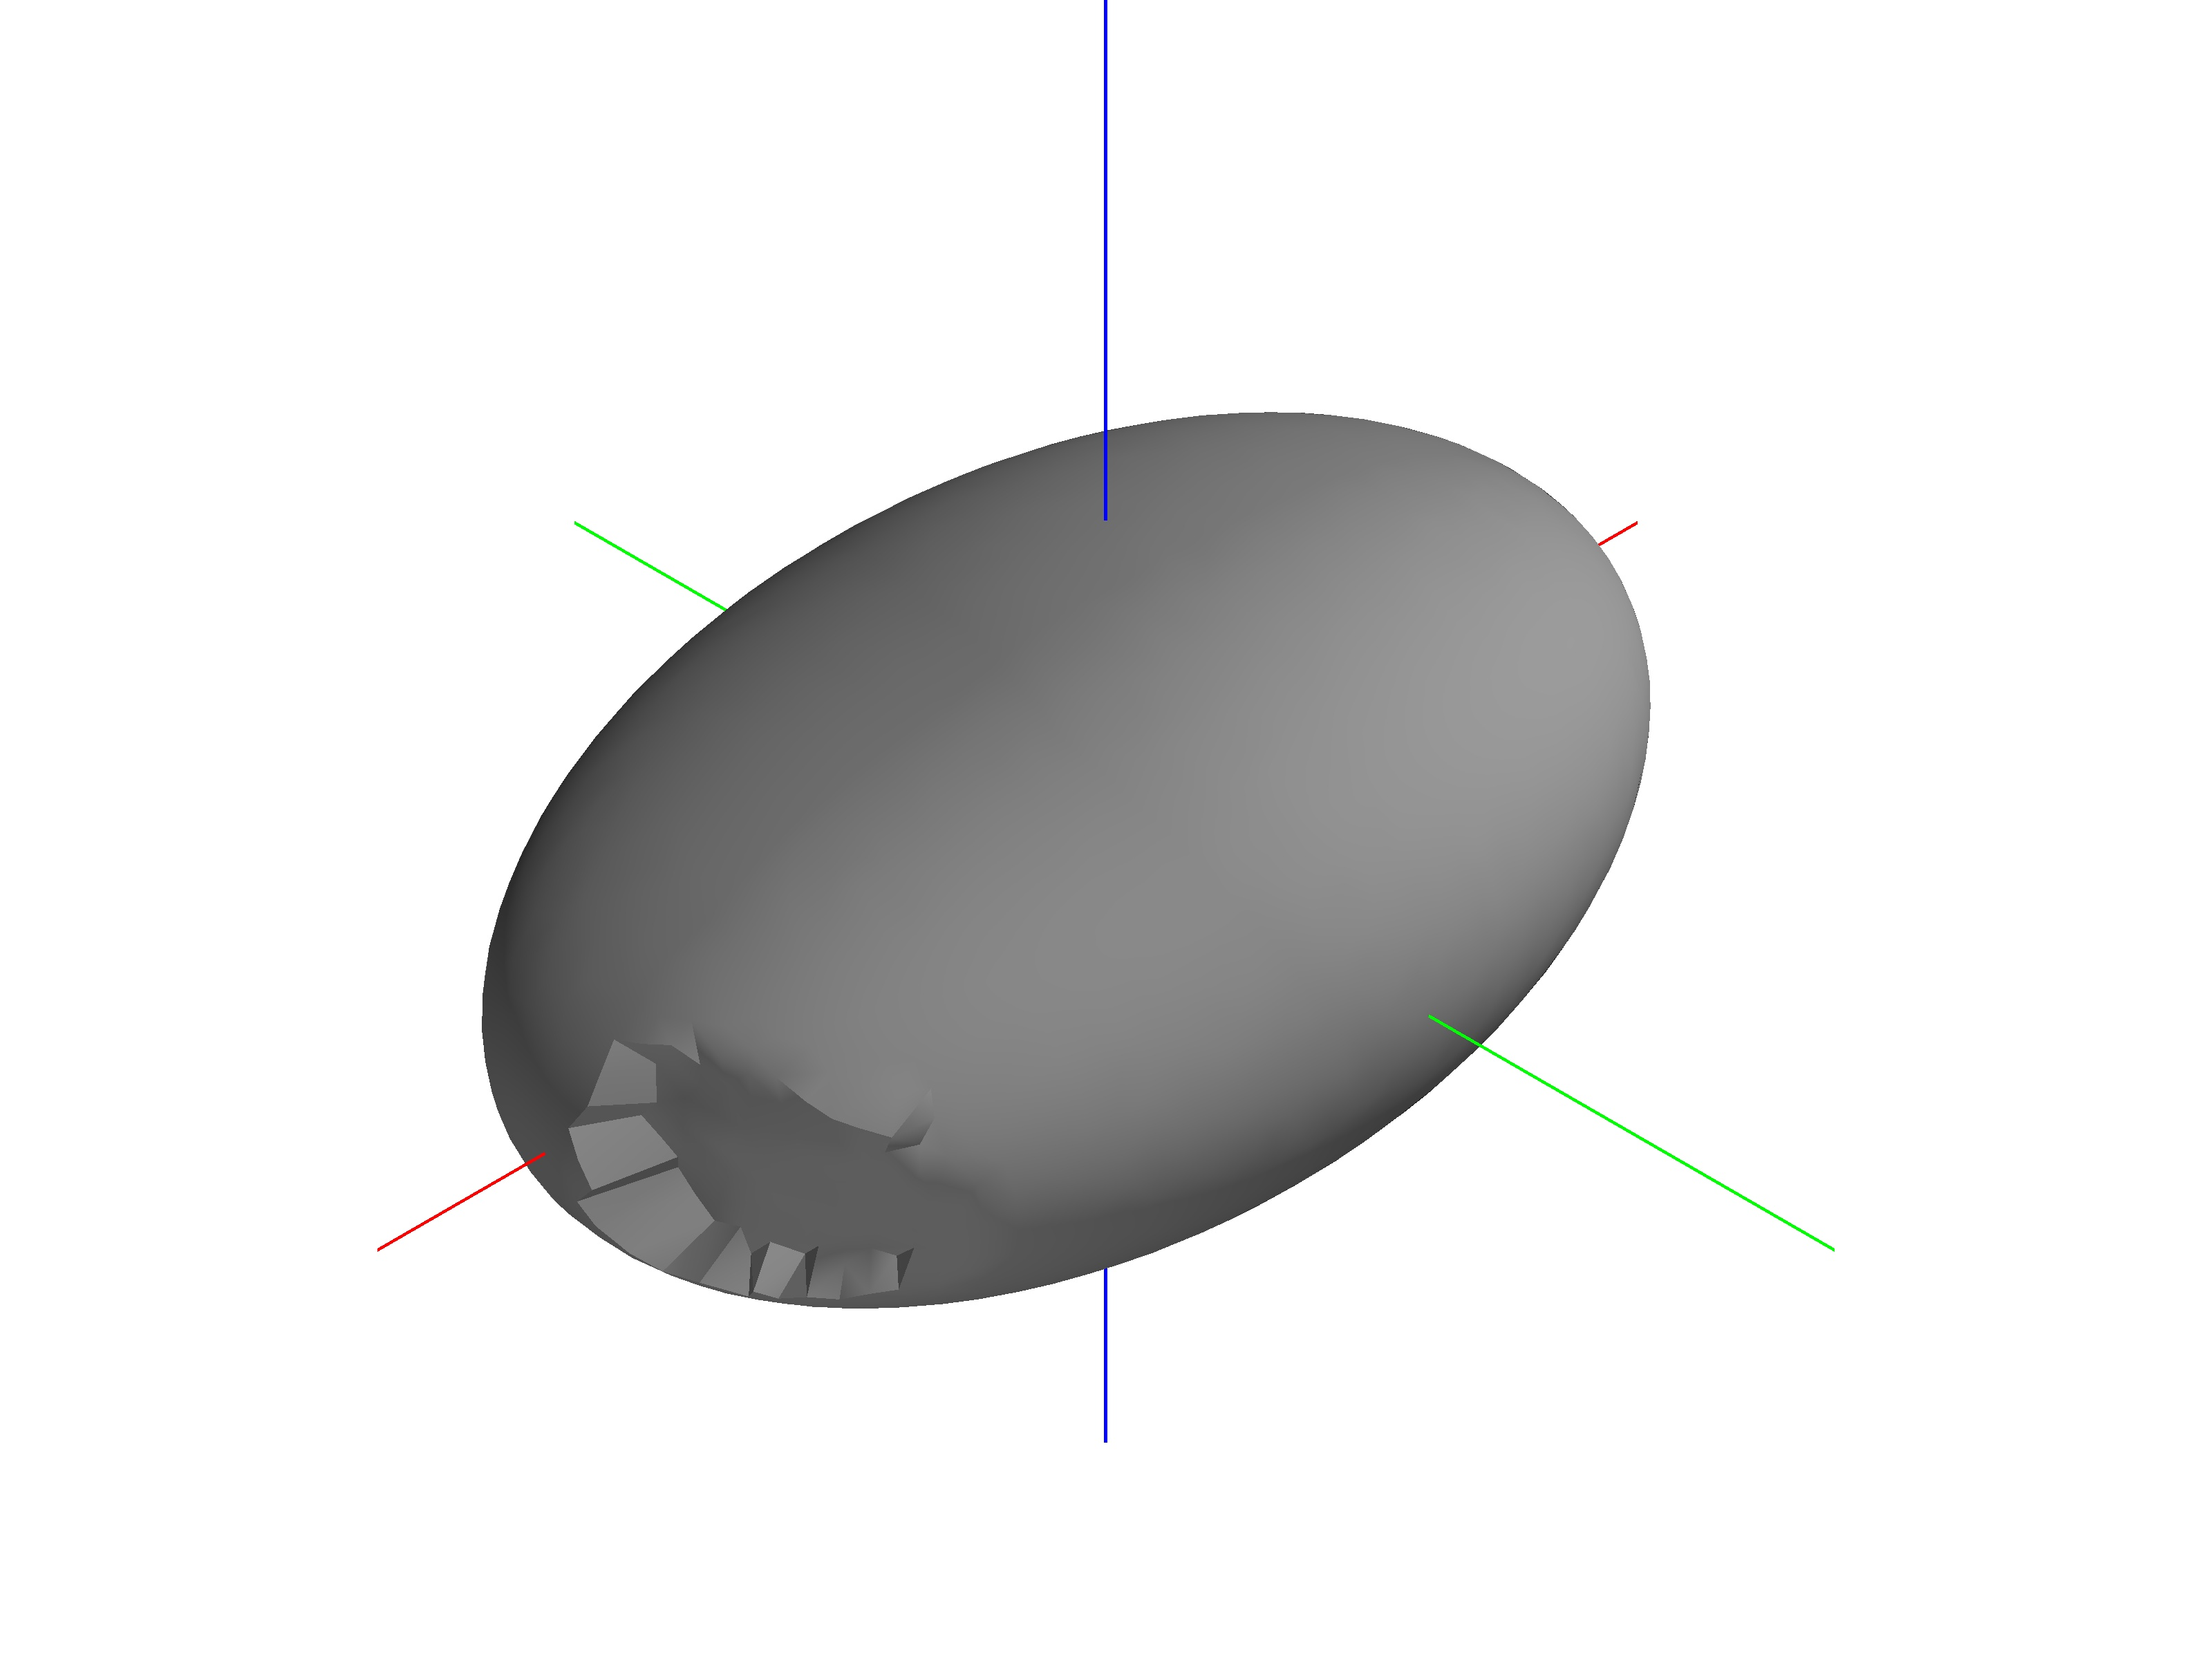
\includegraphics[height=0.5\textheight,width=0.5\textwidth,keepaspectratio]{figures/computational_geometry/dynamic_exploration/castalia/partial_1.jpg}}~
    \subcaptionbox{\SI{25}{\percent} of measurements added\label{fig:castalia_partial_25}}{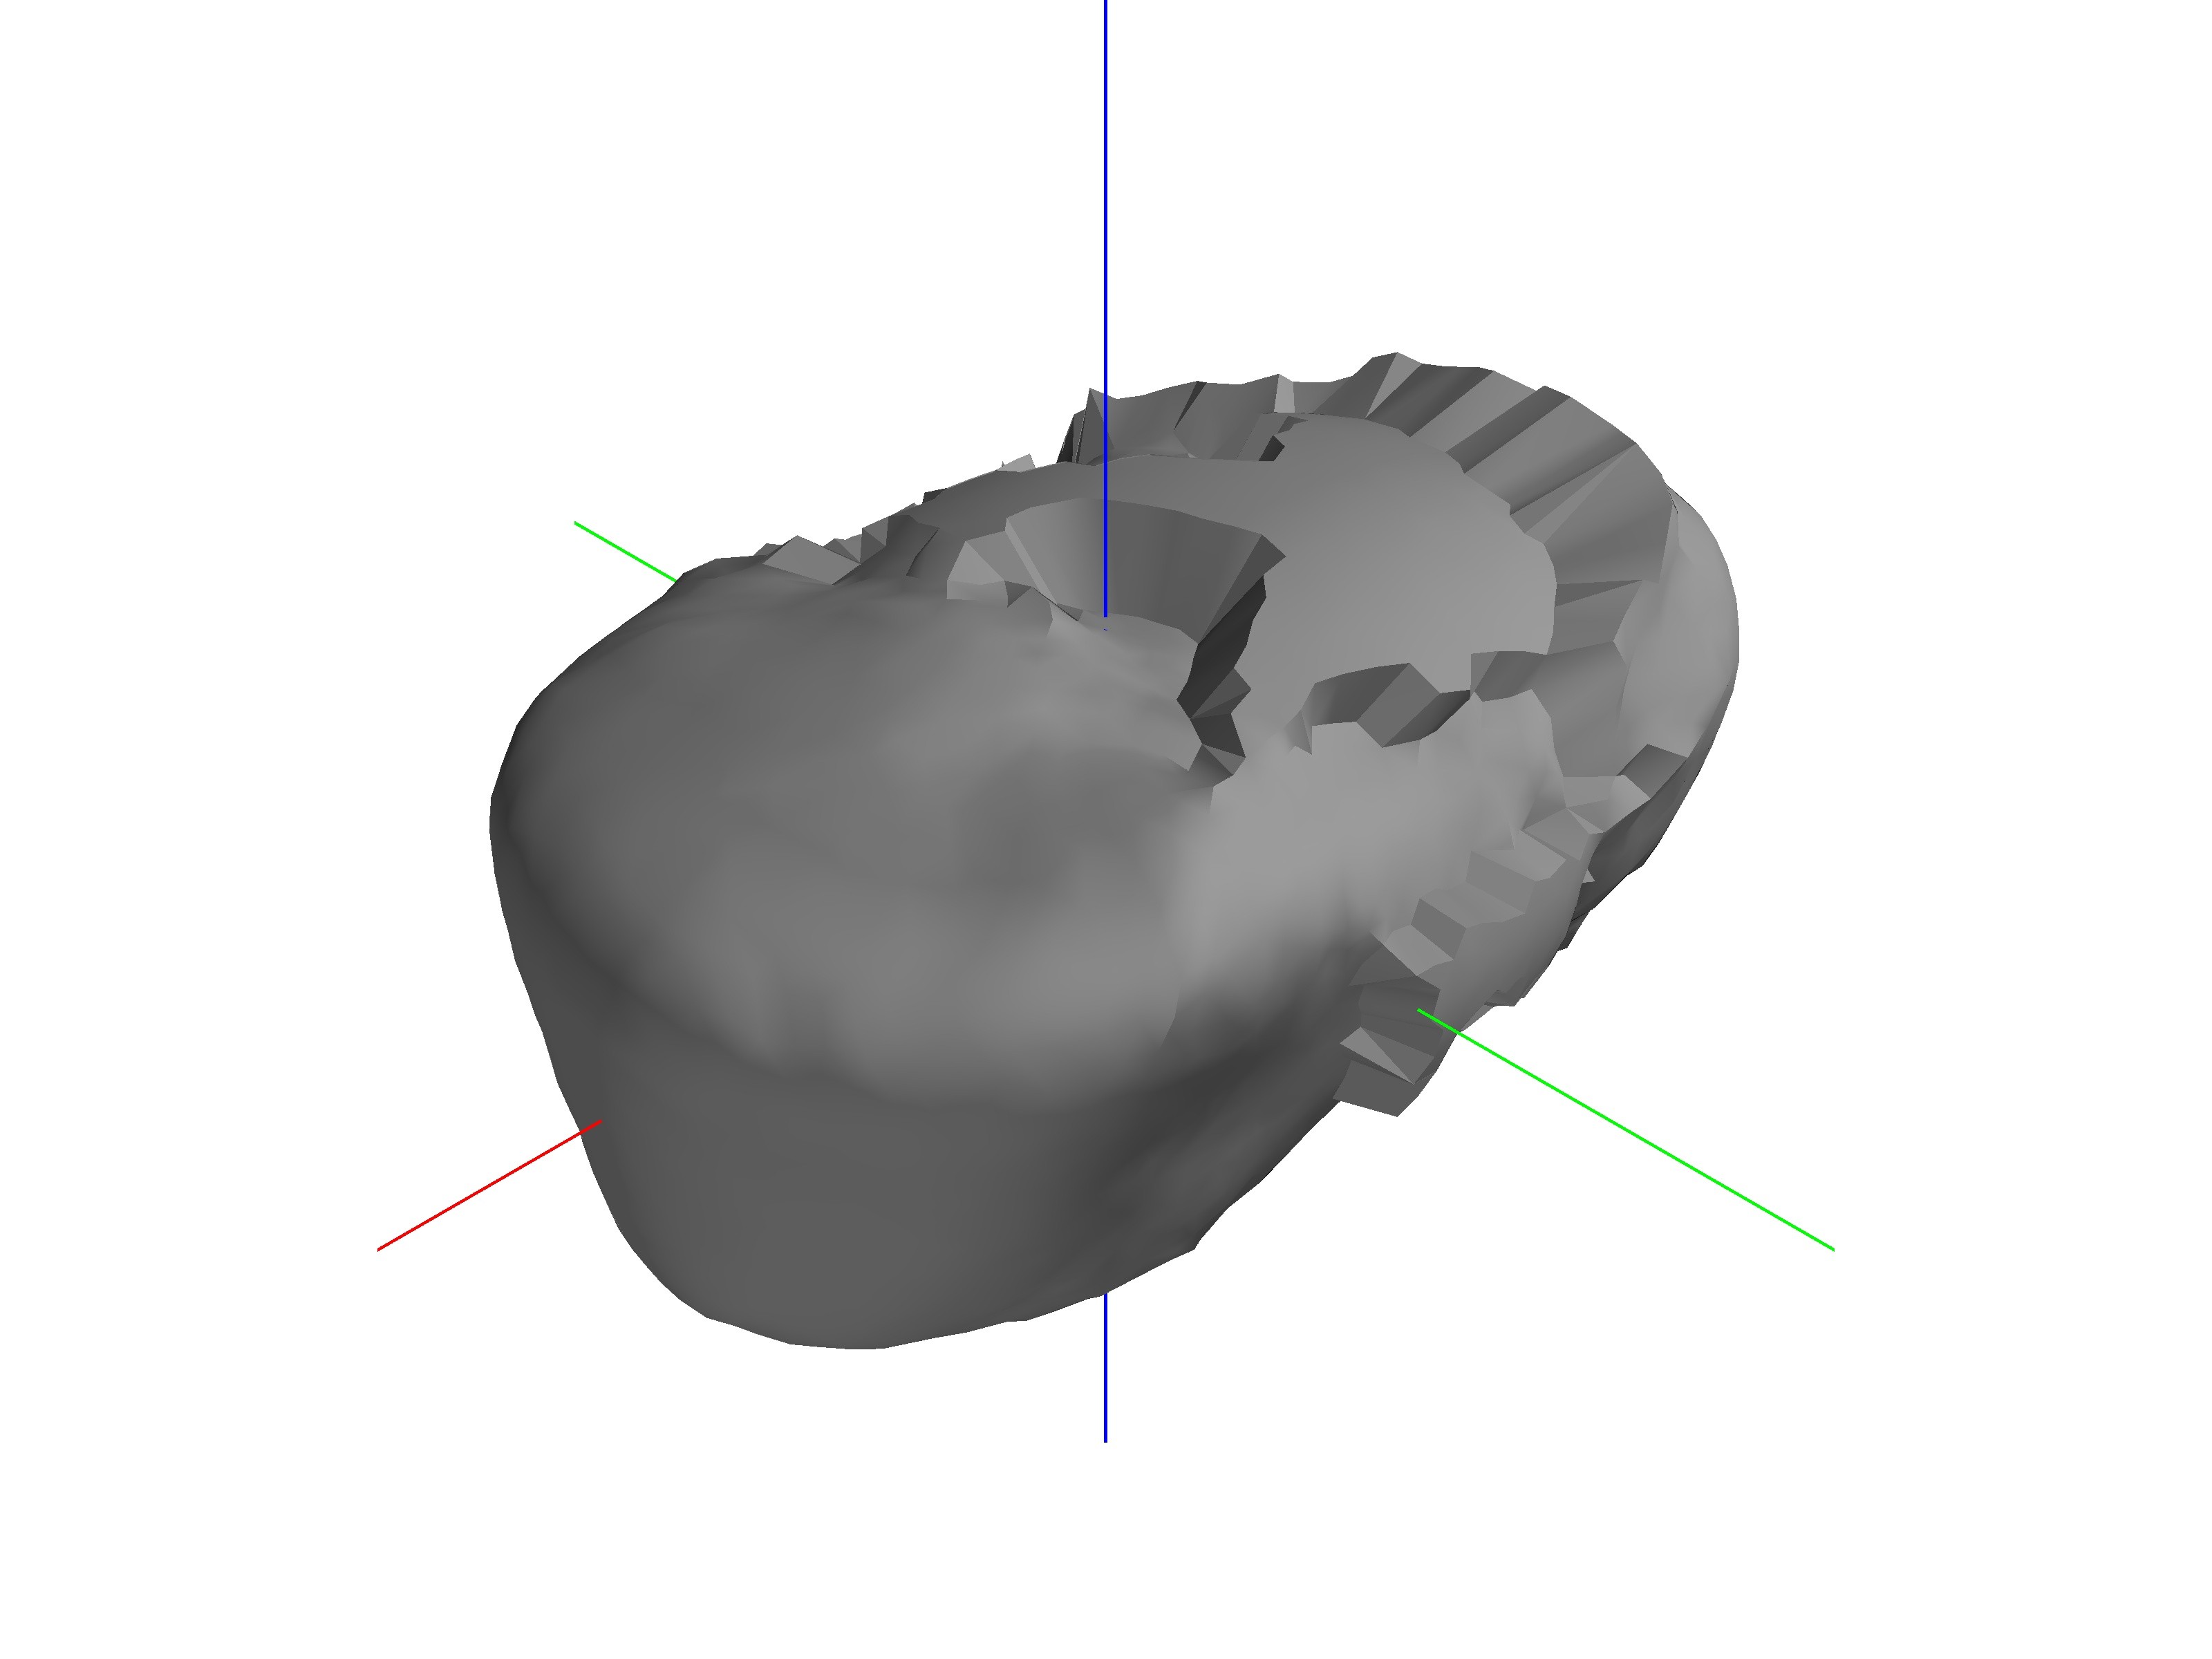
\includegraphics[width=0.5\textwidth]{figures/computational_geometry/dynamic_exploration/castalia/partial_3749.jpg}}

    \subcaptionbox{\SI{50}{\percent} of measurments added\label{fig:castalia_partial_50}}{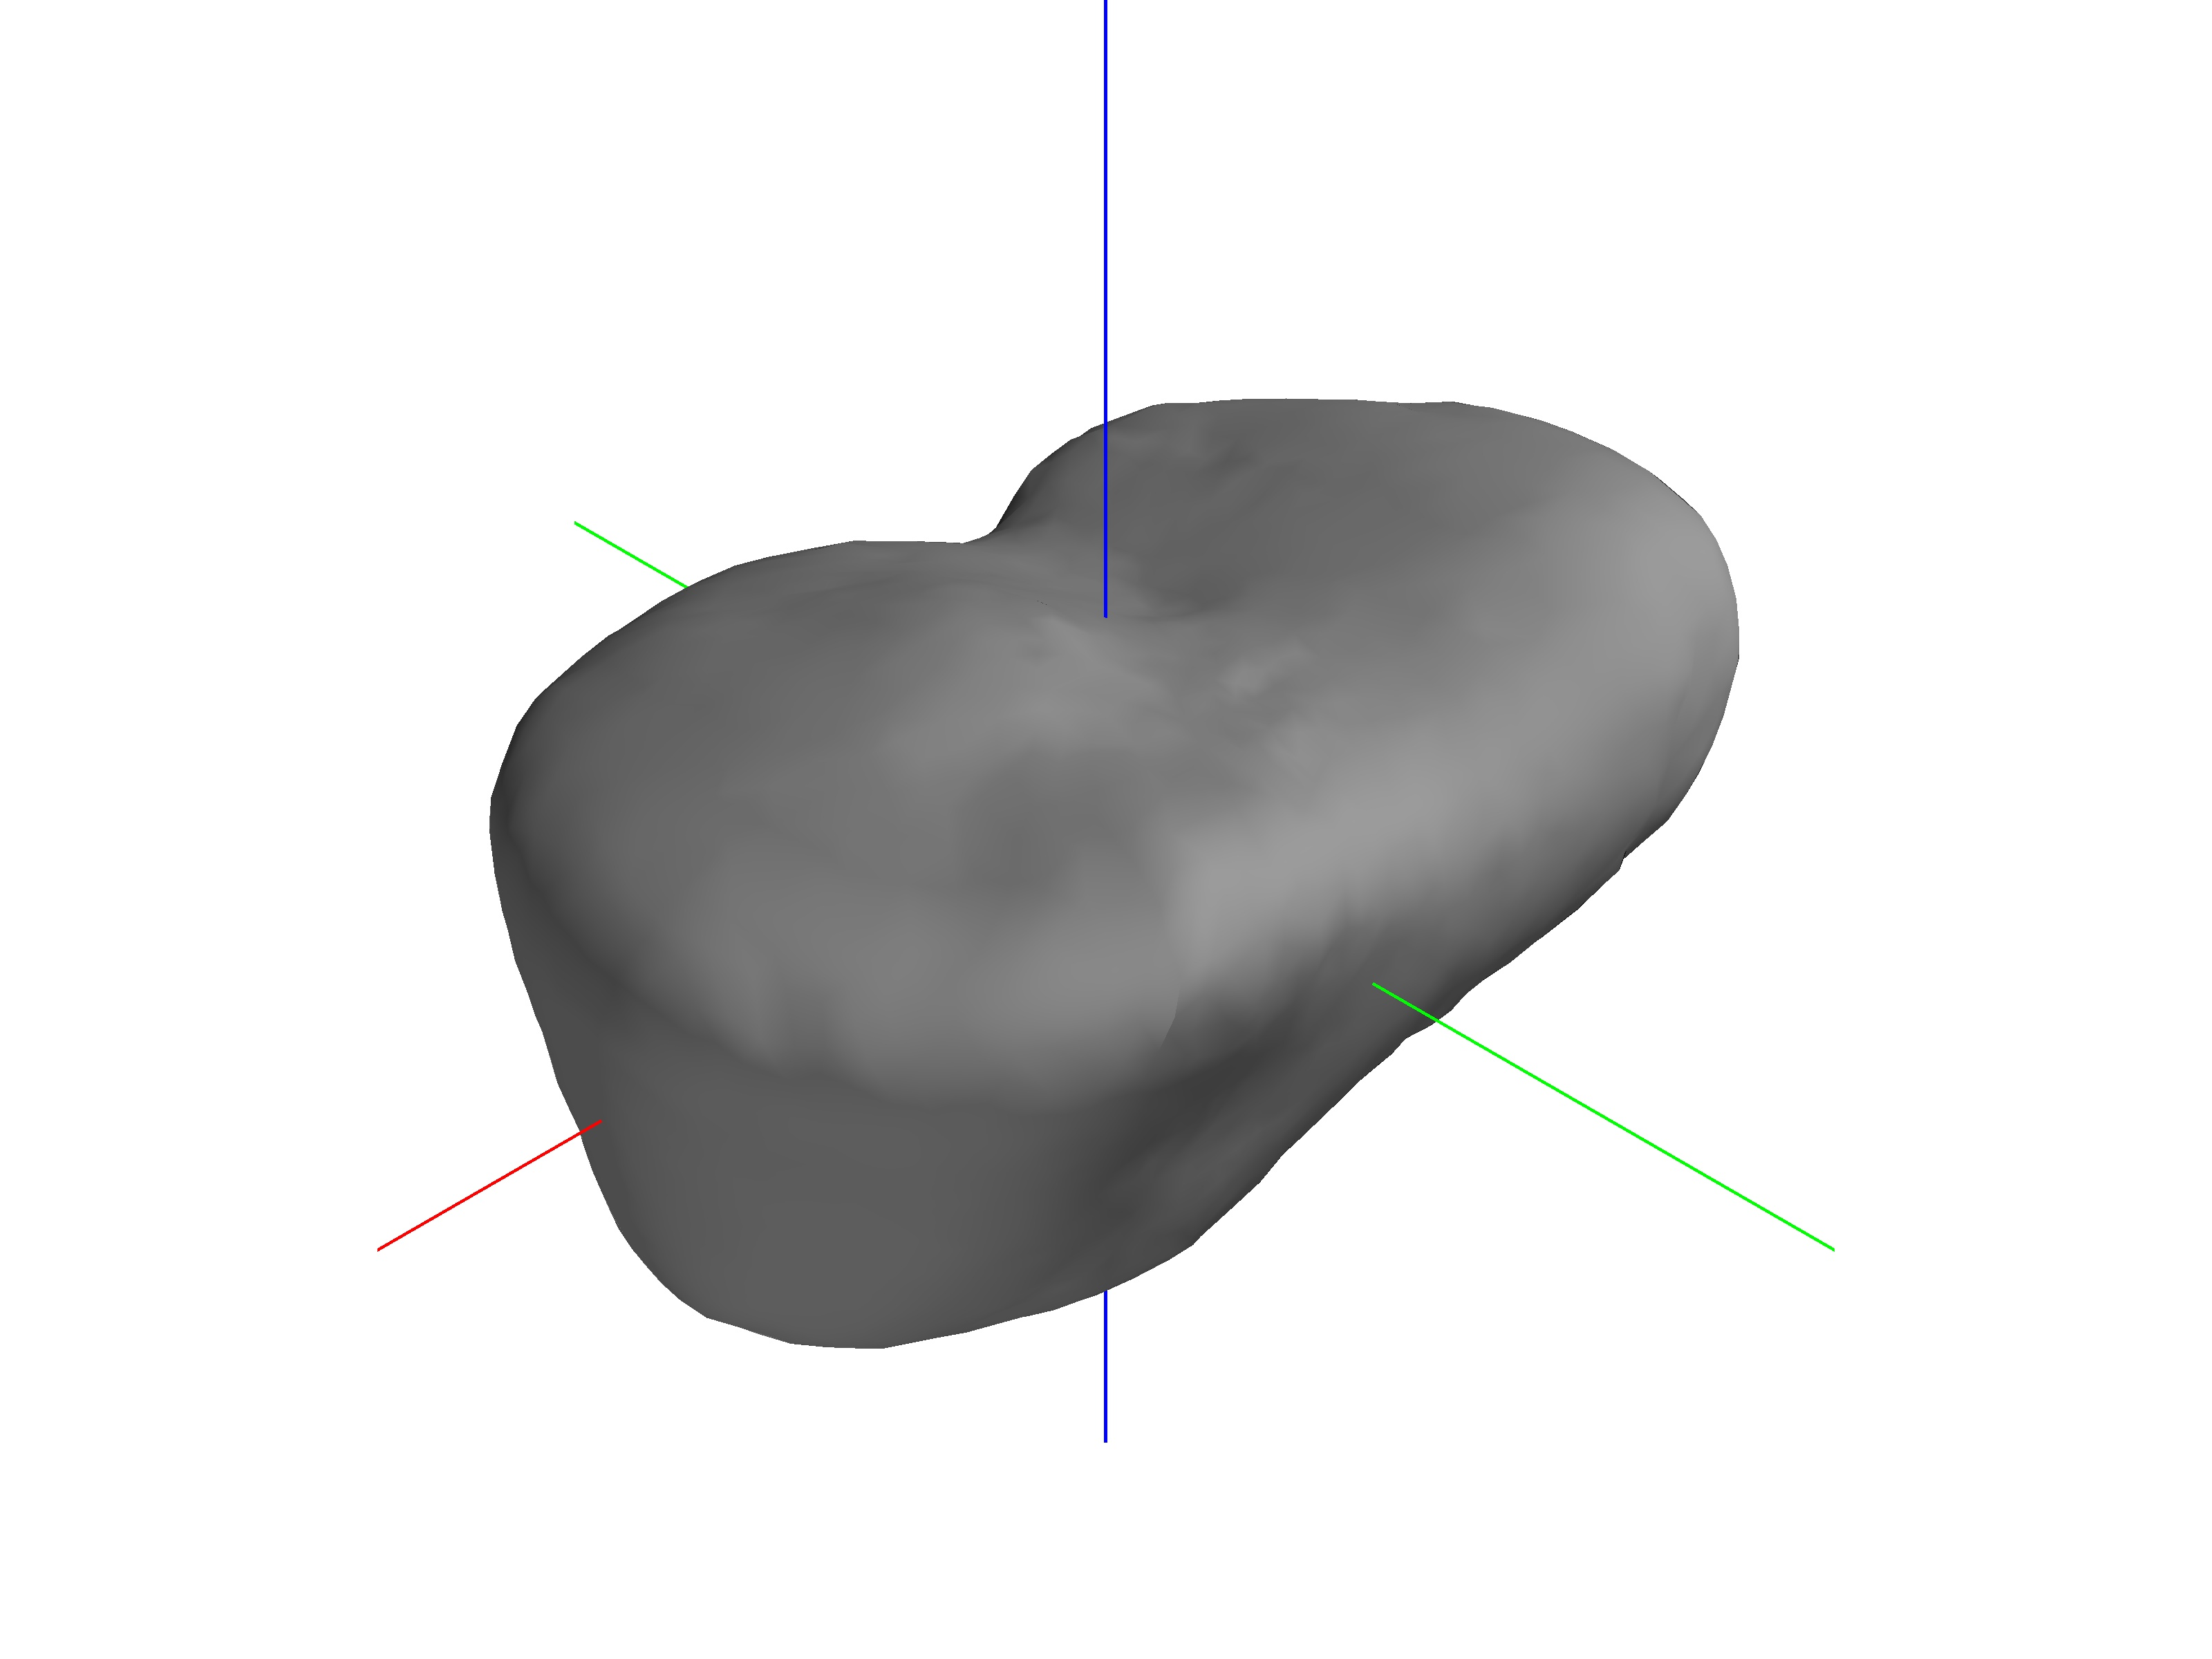
\includegraphics[width=0.5\textwidth]{figures/computational_geometry/dynamic_exploration/castalia/partial_7499.jpg}}~
    \subcaptionbox{\SI{75}{\percent} of measurements added\label{fig:castalia_partial_75}}{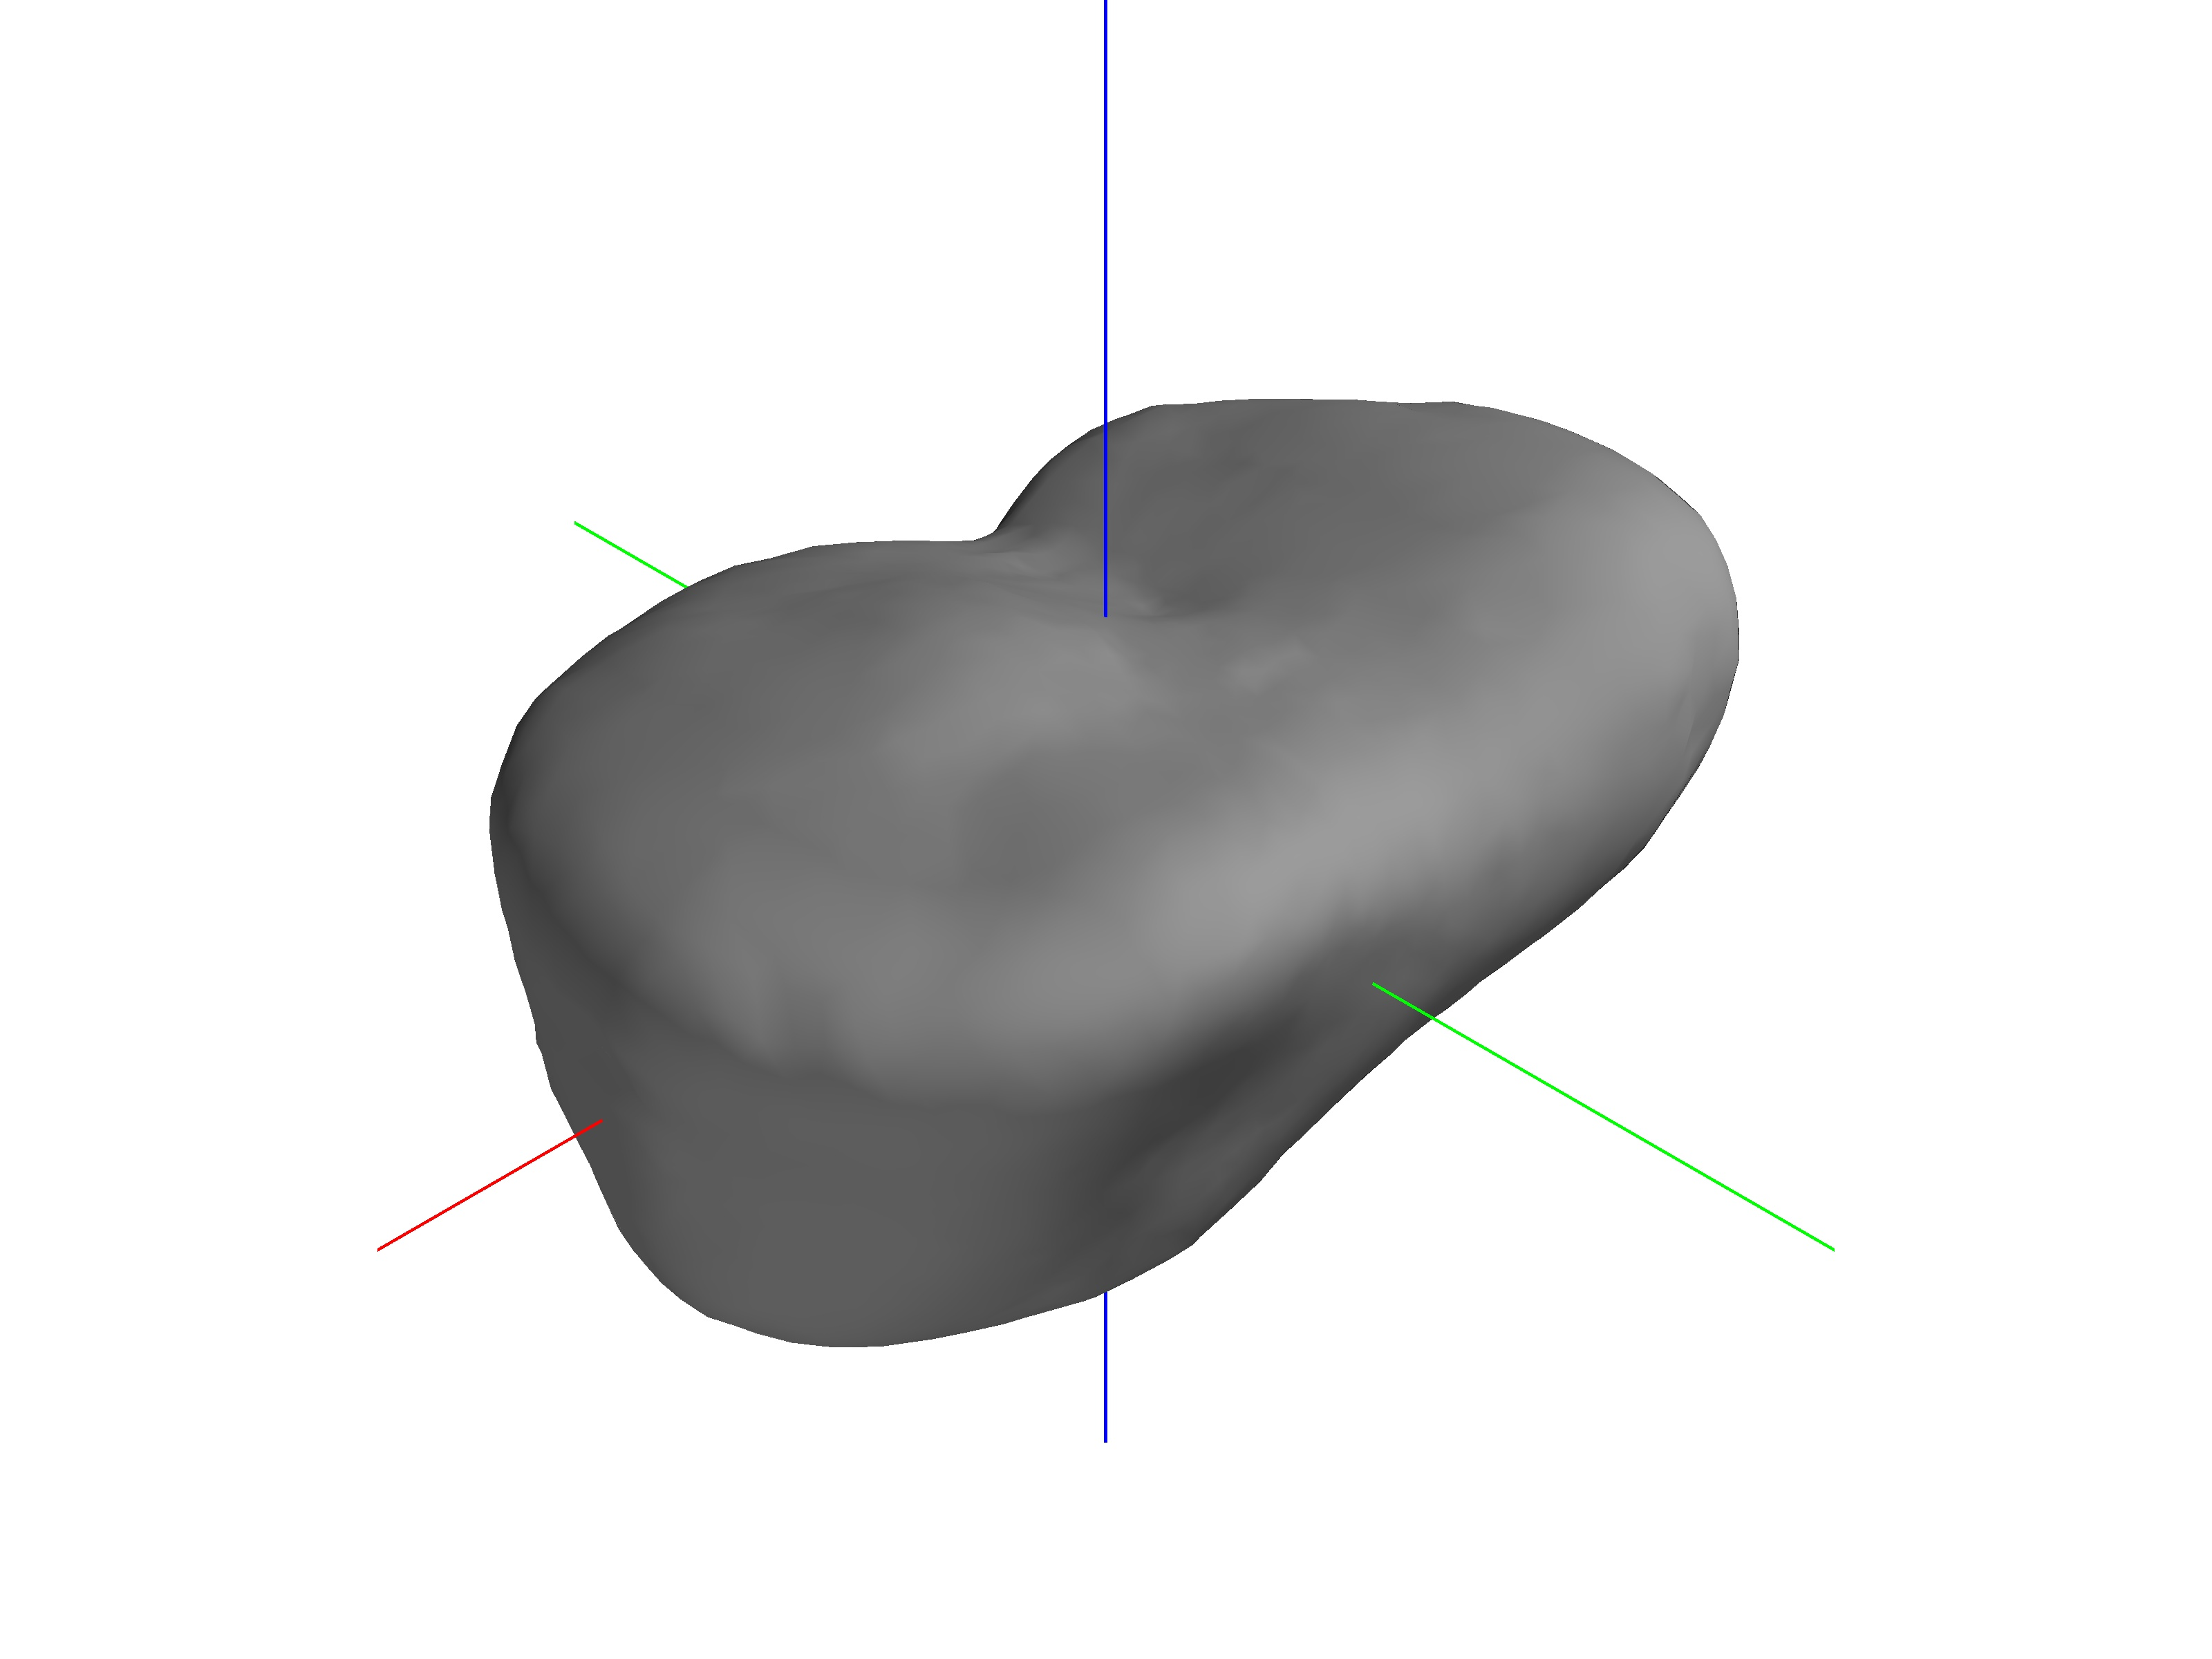
\includegraphics[width=0.5\textwidth]{figures/computational_geometry/dynamic_exploration/castalia/partial_11249.jpg}}

    \subcaptionbox{\SI{100}{\percent} of measurements added\label{fig:castalia_partial_100}}{\includegraphics[width=0.5\textwidth]{figures/computational_geometry/dynamic_exploration/castalia/partial_14998.jpg}}~
    \subcaptionbox{True Shape Model\label{fig:castalia_truth}}{\includegraphics[width=0.5\textwidth]{figures/computational_geometry/mesh_update/castalia/truth.jpg}}
    \caption[Asteroid Castalia Incremental Reconstruction]{Incremental Reconstruction of asteroid Castalia~\label{fig:castalia_reconstruction}}
\end{figure}

\begin{figure}[htbp]
    \centering
    \subcaptionbox{Initial Shape Estimate\label{fig:castalia_partial_weights_0}}{\includegraphics[height=0.5\textheight,width=0.5\textwidth,keepaspectratio]{figures/computational_geometry/dynamic_exploration/castalia/partial_weights_1.jpg}}~
    \subcaptionbox{\SI{25}{\percent} of measurements added\label{fig:castalia_partial_weights_25}}{\includegraphics[width=0.5\textwidth]{figures/computational_geometry/dynamic_exploration/castalia/partial_weights_3749.jpg}}

    \subcaptionbox{\SI{50}{\percent} of measurments added\label{fig:castalia_partial_weights_50}}{\includegraphics[width=0.5\textwidth]{figures/computational_geometry/dynamic_exploration/castalia/partial_weights_7499.jpg}}~
    \subcaptionbox{\SI{75}{\percent} of measurements added\label{fig:castalia_partial_weights_75}}{\includegraphics[width=0.5\textwidth]{figures/computational_geometry/dynamic_exploration/castalia/partial_weights_11249.jpg}}

    \subcaptionbox{\SI{100}{\percent} of measurements added\label{fig:castalia_partial_weights_100}}{\includegraphics[width=0.5\textwidth]{figures/computational_geometry/dynamic_exploration/castalia/partial_weights_14998.jpg}}~
    \subcaptionbox{True Shape Model\label{fig:castalia_weights_truth}}{\includegraphics[width=0.5\textwidth]{figures/computational_geometry/mesh_update/castalia/truth.jpg}}
    \caption[Asteroid Castalia Shape Reconstruction with Uncertainty]{Incremental Reconstruction of asteroid Castalia. The images colored according to the shape uncertainty. Areas of high uncertainty are in yellow while ares of low uncertainty are in purple.~\label{fig:castalia_weights_reconstruction}}
\end{figure}

\Cref{fig:castalia_metrics} shows the total normalized uncertainty and percent error for the volume estimate. 
The plots show that the reconstruction converges to an accurate shape estimate after approximately \SI{8000}{\second}.
In addition, the volume estimate is initially a much larger value but quickly converges to the true value.
\begin{figure}[htbp]
    \centering
    \subcaptionbox{Normalized Uncertainty\label{fig:castalia_uncertainty}}{\includegraphics[width=0.5\textwidth,height=0.31\textwidth]{tikz/castalia_uncertainty.tikz}}~
    \subcaptionbox{Volume Percent Error\label{fig:castalia_volume}}{\includegraphics[width=0.5\textwidth,height=0.31\textwidth]{tikz/castalia_volume.tikz}}
    \caption{Normalized uncertainty and volume percent error for Castalia\label{fig:castalia_metrics}}
\end{figure}

The spacecraft autonomously navigates around asteroid Castalia to best minimize the cost function in~\cref{eq:control_cost}.
The state trajectory is visualized in the asteroid frame in~\cref{fig:castalia_explore_trajectory}.
\begin{figure}[htbp]
    \centering
    \includegraphics[width=\textwidth]{figures/computational_geometry/dynamic_exploration/castalia/state/asteroid_trajectory.jpg}
    \caption{Spacecraft trajectory in the rotating asteroid frame~\label{fig:castalia_explore_trajectory}}
\end{figure}
The component plots of the trajectory are shown in~\cref{fig:castalia_explore_components}.
\begin{figure}[htbp]
    \centering
    \includegraphics[width=\textwidth]{figures/computational_geometry/dynamic_exploration/52760/state/ast_comp.pdf}
    \caption{Components of spacecraft trajectory\label{fig:castalia_explore_components}}
\end{figure}

\paragraph{Castalia Landing Site Selection}
With an appropriate shape estimate, the spacecraft can autonomously transition from a shape reconstruction to a landing mode.
Based on the shape estimate we seek to determine the best location to land. 
In reality, any landing site selection would be based on a wide variety of factors and constraints, however we highlight a few which can be determined autonomously and from the shape estimate.
The first metric is related to the surface slope which is computed using the completed shape estimate and~\cref{eq:surface_slope}.
Areas which violate the slope constraint of \( \phi < \SI{5}{\degree} \) are excluded from further consideration.
\begin{figure}[htbp]
    \centering
    \subcaptionbox{Surface slope of Castalia\label{fig:surface_slope_castalia}}{\includegraphics[width=0.5\textwidth]{figures/computational_geometry/dynamic_exploration/castalia/refine/slope.pdf}}~
    \subcaptionbox{Masked surface slope with areas \( \phi > \SI{5}{\degree}\) excluded\label{fig:surface_slope_castalia_masked}}{\includegraphics[width=0.5\textwidth,keepaspectratio]{figures/computational_geometry/dynamic_exploration/castalia/refine/slope_masked.pdf}}
    \caption{Surface Slope of Asteroid Castalia\label{fig:surface_slope_castalia_both}}
\end{figure}

The next metric is related to the distance from the current spacecraft position to all candidate landing sites on the surface.
We utilize~\cref{eq:geodesic_distance} to compute a distance metric to the surface.
Landing sites which are closely will be considered preferentially over those at a larger distance.
\Cref{fig:distance_castalia_both} shows a surface plot of the distance to the surface. 
The area immediately beneath the spacecraft has a small cost while those on the opposite side of the asteroid have a much larger cost.
\begin{figure}[htbp]
    \centering
    \subcaptionbox{Surface Distance to surface of Castalia\label{fig:surface_distance_castalia}}{\includegraphics[width=0.5\textwidth]{figures/computational_geometry/dynamic_exploration/castalia/refine/dist.pdf}}~
    \subcaptionbox{Masked distance to surface with areas \( \phi > \SI{5}{\degree}\) excluded\label{fig:surface_slope_castalia_masked}}{\includegraphics[width=0.5\textwidth,keepaspectratio]{figures/computational_geometry/dynamic_exploration/castalia/refine/dist_masked.pdf}}
    \caption{Distance to surface of Asteroid Castalia\label{fig:distance_castalia_both}}
\end{figure}
We can combine~\cref{fig:distance_castalia_both,fig:surface_slope_castalia_both} to determine the best landing site. 
The combination of the two is shown in~\cref{fig:landing_site_cost} with the desired landing site shown by the blue marker.
\begin{figure}[htbp]
    \centering
    \includegraphics[width=\textwidth,keepaspectratio]{figures/computational_geometry/dynamic_exploration/castalia/refine/cost.pdf}
    \caption{Total Cost for surface Landing based on surface slope and distance\label{fig:landing_site_cost}}
\end{figure}
After selecting the appropriate landing site we then prepare for landing by collecting more measurements in the region around the landing area.

\paragraph{Castalia Landing Site Refinement}
One key benefit of an in-situ spacecraft is the ability to measure surface features at a much higher resolution than is possible from the ground. 
This detail provides a much higher fidelity data source than ground based measurements. 
In order to emulate this in the simulation we augment the shape model of Castalia with several small craters and outcroppings as shown in~\cref{fig:castalia_bump_true}.
However, these small features would be difficult to capture with the current low resolution shape model of approximately \num{4000} faces.
The lower number of faces is useful for the evaluation of the polyhedron potential model, it is not ideal for the capture of minute surface features. 
As a result, we utilize the isotropic remeshing operation described previously to selectively increase the fidelity in the region about the desired landing site.
\Cref{fig:castalia_refine_density} shows that the vertex density increases by approximately an order of magnitude in region immediately surround the landing site.
\begin{figure}[htbp]
    \centering
    \subcaptionbox{Original vertex density of the initial shape estimate\label{fig:intial_vertex_density}}{\includegraphics[width=1.0\textwidth]{figures/computational_geometry/dynamic_exploration/castalia/refine/density.pdf}}

    \subcaptionbox{Vertex density after refinement  around landing site\label{fig:refine_vertex_density}}{\includegraphics[width=1.0\textwidth]{figures/computational_geometry/dynamic_exploration/castalia/land/density.pdf}}
    \caption{Vertex density before and after refinement at asteroid Catalia\label{fig:castalia_refine_density}}
\end{figure}

The increased number of faces and vertices in the landing area allows for the capture of the small surface features.
\Cref{fig:castalia_bump_est} shows that given \gls{lidar} measurements alone and the algorithm presented in~\cref{sec:radius_update} the small craters and features are effectively estimated.
\begin{figure}[htbp]
    \centering
    \subcaptionbox{True Shape model with surface features\label{fig:castalia_bump_true}}{\includegraphics[width=0.5\textwidth]{figures/computational_geometry/dynamic_exploration/castalia_bump_true.jpg}}~
    \subcaptionbox{Estimated Shape model after refinement\label{fig:castalia_bump_est}}{\includegraphics[width=0.5\textwidth]{figures/computational_geometry/dynamic_exploration/castalia_bump_est.jpg}}
    \caption{Asteroid Castalia with augmented with additional surface features~\label{fig:castalia_refinement}}
\end{figure}

\paragraph{Castalia Vertical Descent}
The final phase of the simulation is to utilize the mixed resolution model and vertically descend to the desired landing site. 
This is accomplished using the closed loop control of~\cref{sec:se3_control} and a trajectory which transitions from the home postion to the surface over \SI{3600}{\second}.
The landing trajectory, using the estimated shape, is visualized in the asteroid frame in~\cref{fig:castalia_landing}.
\begin{figure}[htbp]
    \centering
    \includegraphics[width=\textwidth]{figures/computational_geometry/dynamic_exploration/castalia/land/asteroid_trajectory.jpg}
    \caption{Vertical descent onto 4769 Castalia~\label{fig:castalia_landing}}
\end{figure}
